% ===================================================================
%  TASI Lectures on Moonshine —— 中文译注版（完整单文件源码）
%  底本：V. Anagiannis & M. C. N. Cheng, arXiv:1807.00723v1 [hep-th]
%  编译：xelatex（需 ctex；两遍生成目录）；本文件自包含，仅 figures/ 外部依赖。
%  % [Tutor Note: ...] 为译者批注（LaTeX 注释，不影响排版）。
% ===================================================================
% ===================================================================
%  TASI Lectures on Moonshine —— 中文译注版（主文件）
%  底本：V. Anagiannis, M. C. N. Cheng, arXiv:1807.00723v1 [hep-th]
%  编译：XeLaTeX（ctex），两遍以生成目录与交叉引用
% ===================================================================
\documentclass[11pt,a4paper,fontset=windows]{ctexart}


% ---------- 页面与版式 ----------
\usepackage[a4paper,total={150mm,257mm},left=35mm,right=35mm,top=30mm,bottom=30mm]{geometry}
\pagestyle{plain}
\linespread{1.08}
\setlength{\emergencystretch}{2em}

% ---------- 数学与符号 ----------
\usepackage{amsmath,amssymb,amsfonts,mathtools,latexsym,amsthm}
\allowdisplaybreaks[1]
\usepackage{dsfont}          % \mathds{1}
\usepackage{graphicx}
\usepackage{caption}
\captionsetup{font=small,labelfont=bf,labelsep=quad}
\usepackage{array}
\usepackage{xcolor}
\usepackage{enumitem}
\usepackage{authblk}
\usepackage{hyperref}
\hypersetup{
  colorlinks=true,
  linkcolor=blue!55!black,
  citecolor=blue!55!black,
  urlcolor=magenta!70!black,
  bookmarksnumbered=true,
  pdftitle={TASI 月光讲义（中文译注版）},
  pdfauthor={Vassilis Anagiannis, Miranda C. N. Cheng; 中译/译注}
}

% ---------- 定理类环境（与原文章节编号一致） ----------
\newtheorem{thm}{定理}[section]
\newtheorem{conj}[thm]{猜想}
\newtheorem{proposition}[thm]{命题}
\newtheorem{claim}[thm]{断言}
\newtheorem{lemma}[thm]{引理}
\numberwithin{equation}{section}

% ---------- “本节重点（Key Takeaways）” 版式 ----------
\newenvironment{keytakeaways}
  {\par\medskip\noindent
   \begin{minipage}{\linewidth}
   \hrule height 0.8pt\smallskip
   \noindent{\bfseries 本节重点（Key Takeaways）}\par\smallskip
   \begin{itemize}[leftmargin=1.6em,itemsep=2pt,topsep=1pt,parsep=0pt,partopsep=0pt]}
  {\end{itemize}\smallskip\hrule height 0.8pt\end{minipage}%
   \par\medskip}

% ===================================================================
%  以下宏定义逐字照搬原文（正文公式依赖这些缩写，切勿改动）
% ===================================================================
\newcommand{\PSL}{\operatorname{\textsl{PSL}}}    %PSL group
\newcommand{\SL}{\operatorname{\textsl{SL}}}      %SL group
\newcommand{\GL}{\operatorname{\textsl{GL}}}      %GL group
\newcommand{\SO}{\operatorname{\textsl{SO}}}      %SO group
\newcommand{\UU}{\operatorname{\textsl{U}}}      %U group
\newcommand{\Co}{\operatorname{\textsl{Co}}}      %Co group
\newcommand{\Th}{\operatorname{\textsl{Th}}}      %Th group
\newcommand{\End}{\operatorname{\text{End}}}      %Endomorphism
\newcommand{\Aut}{\operatorname{\text{Aut}}}      %Endomorphism

\newcommand{\eg}{{\bf EG}}
\newcommand{\modgrp}{{\mathfrak G}_g}

\newcommand*{\bcdot}{\raisebox{-0.6ex}{\scalebox{2}{$\cdot$}}}
\newcommand{\myparagraph}[1]{\paragraph{#1}\mbox\\}
\newcommand{\wk}{{\rm wk}}
\newcommand{\CC}{\mathbb{C}}
\newcommand{\RR}{\mathbb{R}}
\newcommand{\QQ}{\mathbb{Q}}
\newcommand{\FF}{\mathbb{F}}
\newcommand{\HH}{\mathbb{H}}
\newcommand{\ZZ}{\mathbb{Z}}
\newcommand{\Dp}{\mathbb{D}^+}
\newcommand{\Dm}{\mathbb{D}^-}
\newcommand{\PP}{\mathbb{P}}
\newcommand{\MM}{\mathbb{M}}
\newcommand{\TT}{\mathbb{T}}
\newcommand{\Cl}{\text{Cl}}
\newcommand{\A}{\mathcal{A}}
\newcommand{\B}{\mathcal{B}}
\newcommand{\C}{\mathcal{C}}
\newcommand{\E}{\mathcal{E}}
\newcommand{\F}{\mathcal{F}}
\newcommand{\G}{\mathcal{G}}
\newcommand{\Ha}{\mathcal{H}}
\newcommand{\Hh}{\mathcal{H}}
\newcommand{\I}{\mathcal{I}}
\newcommand{\J}{\mathcal{J}}
\newcommand{\Li}{\mathcal{L}}
\newcommand{\M}{\mathcal{M}}
\newcommand{\N}{\mathcal{N}}
\newcommand{\Q}{\mathcal{Q}}
\newcommand{\R}{\mathcal{R}}
\newcommand{\calS}{\mathcal{S}}
\newcommand{\T}{\mathcal{T}}
\newcommand{\V}{\mathcal{V}}
\newcommand{\W}{\mathcal{W}}
\newcommand{\Z}{\mathbb{Z}}
\newcommand{\xmod}{{\rm \;mod\;}}

\newcommand{\RS}{\widehat{\CC}}
\newcommand{\vir}{\mathfrak{Vir}}
\newcommand{\witt}{\mathfrak{Witt}}

\def\a{\alpha}
\def\b{\beta}
\def\c{\gamma}
\def\d{\delta}
\def\dd{\delta}
\def\dbar{\bar{\partial}}
\def\e{\epsilon}
\def\f{\phi}
\def\vf{\varphi}

\def\i{\iota}
\def\im{\mathrm{Im}}
\def\mm{^{(m)}}
\def\inf{\infty}
\def\j{\psi}
\def\k{\kappa}
\def\l{\lambda}
\def\m{\mu}
\def\n{\nu}
\def\na{\nabla}
\def\o{\omega}
\def\w{\omega}
\def\p{\pi}
\def\pa{\partial}
\def\re{\mathrm{Re}}
\def\r{\rho}
\def\rr{\rho}
\def\s{\sigma}
\def\t{\tau}
\def\taubar{\bar \tau}
\def\tbar{\bar \tau}
\def\th{\theta}
\def\til{\tilde}
\def\u{\upsilon}
\def\v{\varphi}
\def\x{\chi}
\def\we{\wedge}
\def\z{\zeta}
\def\zb{\bar{z}}
\def\D{\Delta}
\def\F{\Phi}

\def\J{\Psi}
\def\L{\Lambda}
\def\O{\Omega}
\def\P{\Pi}
\def\Q{\Theta}
\def\Sig{\Sigma}
\def\T{\Theta}
\def\Tr{\tr}
\def\U{\Upsilon}
\def\X{\Xi}

\newcommand{\normord}[1]{\vcentcolon\mathrel{#1}\vcentcolon}

\newcommand{\ex}{\operatorname{e}} %Number theory exp
\newcommand{\sk}{{\rm sk}}
\newcommand{\g}{\mathfrak{g}}
\newcommand{\h}{\mathfrak{h}}
\newcommand{\tr}{\operatorname{Tr}}
\newcommand{\str}{\operatorname{Str}}
\newcommand{\ext}{\mathsf{\Lambda}}
\newcommand{\Ex}{\operatorname{Ex}}

\newcommand{\rrangle}{\rangle\!\!\!\;\rangle}
\newcommand{\llangle}{\langle\!\!\!\;\langle}

\renewcommand{\labelenumii}{(\roman{enumii})}

\newcommand{\ch}{\text{ch}}

\newcommand{\bea}{\begin{eqnarray}}
\newcommand{\eea}{\end{eqnarray}}
\newcommand{\bee}{\begin{eqnarray*}}
\newcommand{\eee}{\end{eqnarray*}}
\newcommand{\al}{\begin{align*}}
\newcommand{\eal}{\end{align*}}
\newcommand{\be}{\begin{equation}}
\newcommand{\ee}{\end{equation}}
\newcommand{\eq}[1]{(\ref{#1})}
\newcommand{\bem}{\begin{pmatrix}}
\newcommand{\eem}{\end{pmatrix}}

\newcommand\BigBox{\vcenter{\hbox{\scalebox{1.6}{$\Box$}}}}
\newcommand\bigsquare{\mathop{\BigBox}\limits}
\newcommand\boxnot[2]{\vcenter{\hbox{$\textstyle #1$}}{\bigsquare_{\textstyle #2}}}


\begin{document}

% ---------------- 标题页 ----------------
\title{%
  \vspace{-35pt}
  \textsc{\huge TASI Lectures on Moonshine}\\[8pt]
  \Large TASI 月光讲义\\[2pt]
  \large（中文译注版）}
\author[1]{Vassilis Anagiannis\thanks{[邮箱隐去]}}
\author[1,2]{Miranda C. N. Cheng\thanks{[邮箱隐去]}}
\affil[1]{阿姆斯特丹大学物理研究所，荷兰阿姆斯特丹}
\affil[2]{阿姆斯特丹大学 Korteweg--de Vries 数学研究所，荷兰阿姆斯特丹}
\date{}
\maketitle

% ---------------- 摘要 ----------------
\begin{abstract}
\normalsize
“月光”（moonshine）一词在数学中指的是一类出人意料的联系：它把两个看似毫不相干的结构
——有限群表示与模对象（modular objects）——联系在一起。人们相信理解月光现象的关键在于
具有特殊对称性的物理理论。近年来，有限群表示与模对象之间出现了多种新的联系方式，这些进展
既为弦论界带来了希望，也带来了谜题。

本讲义旨在把理论物理与数学物理方向的研究生带到这一活跃研究方向的前沿。第二部分综述各种
月光联系，从上一世纪建立的经典魔群月光（monstrous moonshine）到最新的发现；第三部分讨论
月光联系与物理（尤其是弦论）之间的关系：在简要回顾魔群月光的一个近期物理实现之后，我们将
较详细地描述本影月光（umbral moonshine）物理面向之谜，并提及弦论黑洞与月光相联系的其他
若干情形。为使内容自足，第一部分还提供了必要的背景知识，包括有限群、模对象与二维共形场论；
这一部分占全部篇幅的一半，熟悉相关概念与技巧的读者可以跳过。
\end{abstract}

\newpage

% ---------------- 译者说明 ----------------
\section*{译者说明}
\addcontentsline{toc}{section}{译者说明}

\begin{enumerate}[label=\arabic*.,leftmargin=2.2em,itemsep=3pt]
\item \textbf{底本。}本译文的底本为 Vassilis Anagiannis 与 Miranda C. N. Cheng 的
      \emph{TASI Lectures on Moonshine}（arXiv:1807.00723v1 [hep-th]，2018 年 7 月 2 日；
      78 页），系作者在 TASI 2017 暑期学校所作讲座的讲义。原文中“原书 p.N”均指该 PDF 的
      页码（PDF 页码与印刷页码一致）。

\item \textbf{翻译原则。}公式一律照原文逐符号保留，不做任何“顺手改写”；原文若有笔误或
      记号冲突，译文保持原样并以 \verb|% [Tutor Note: ...]| 批注说明。术语以中文学界通行
      译名为准，首次出现处括注英文原词；无稳定中译的术语（如 mock modular form 之外的
      twining 等）保留英文。参考文献保持英文原貌，仅作必要的位置调整。

\item \textbf{批注体例。}正文中的 LaTeX 注释 \verb|% [Tutor Note: ...]| 为译者批注，
      分三类：\emph{易错预警}（指标、符号、约定）、\emph{含糊点拨}（作者以“显然”“易得”
      带过的论证）与\emph{背景直觉}。批注是源码注释，不影响编译与排版，便于读者在源码中
      逐条查阅。

\item \textbf{图表。}原文三幅插图（图 1--3）与一张表格已从 PDF 中单独裁出，存于
      \verb|figures/| 目录；图注译为中文并标注原文页码。插图内的英文标注（如
      “Modular forms”“Finite groups”）为保持与原文一致未作改动，其含义见图注。

\item \textbf{编译。}建议使用 XeLaTeX 编译两遍：\verb|xelatex main.tex|。中文排版由
      \texttt{ctex} 宏包（Windows 字体集）处理；若在无 Windows 字体的系统上编译，可将
      文档类选项 \verb|fontset=windows| 改为 \verb|fontset=fandol|。
\end{enumerate}

\newpage

% ---------------- 目录 ----------------
\tableofcontents
\newpage

% ---------------- 正文 ----------------

% ==================== 内联自 chapters/ch00_intro.tex ====================
% ===================================================================
%  导言（Introduction） 原文：TASI10.tex 第 213--293 行（PDF p.2--5）
% ===================================================================
\section*{导言}

“月光”（moonshine）一词在数学中用来指模对象与有限群表示之间一种出人意料的联系。
过去五年间，对月光现象的研究进展迅速。这一联系虽然发生在两个数学结构之间，
人们却预期这种奇特联系的根源在物理，尤其是在弦论之中。

\vspace{2pt}
\begin{figure}[h!]
  \begin{center}
    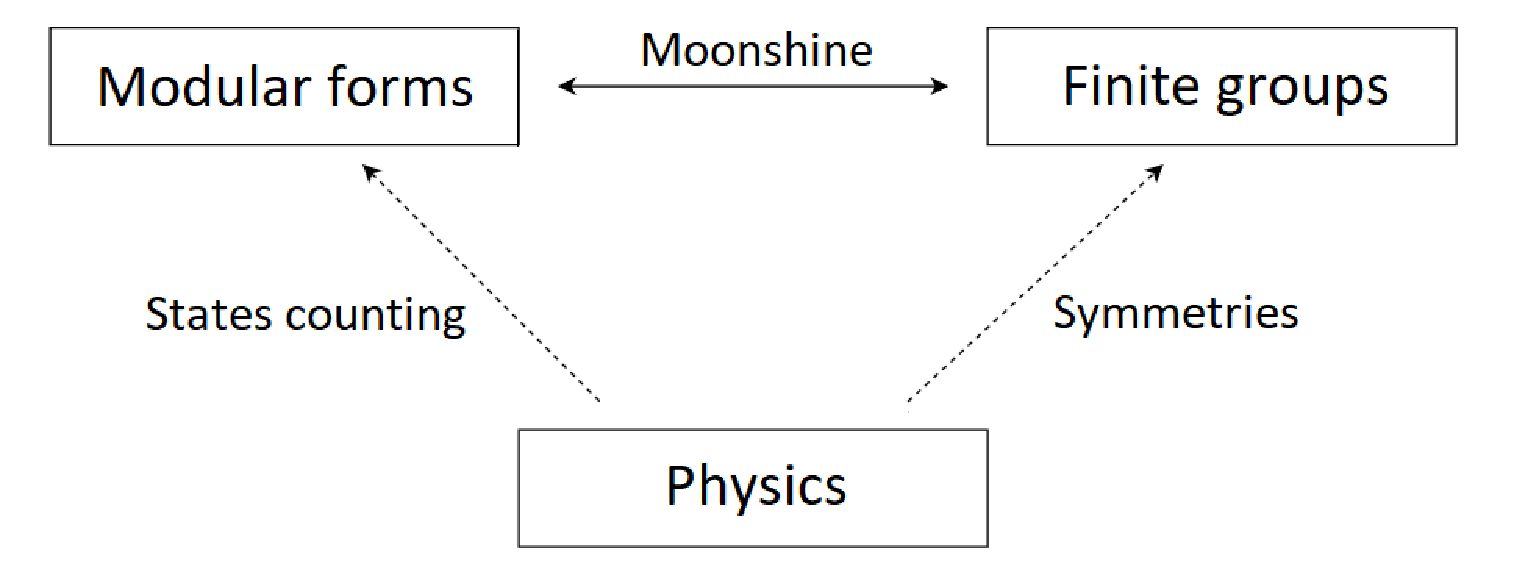
\includegraphics[width=0.66\linewidth]{figures/fig1_moonshine_diagram.pdf}
    \caption*{月光示意图。上方双向箭头表示模形式与有限群之间的“月光”联系；
    下方两条虚线分别表示“态计数”（states counting）与“对称性”（symmetries），
    意指两侧结构都通过物理（尤其是弦论）得到解释。原文此图无图注，位置见原文 p.2；
    本图注为译者所加，图中英文标注保持原样。}
  \end{center}
\end{figure}
\vspace{-8pt}

% [Tutor Note: “moonshine”一词由 Conway 与 Norton 在 1979 年引入，本义是“空谈、异想天开”，
% 用在此处带自嘲意味：两个毫不相干的数学结构竟由同一组整数联系起来，起初像是无稽之谈。
% 中文“月光”是约定俗成的译法，不要译作“月光效应”。]

\subsection*{月光：是什么、如何产生、为何重要？}

{\bf \em 问：什么是月光？}
\\\noindent
模形式的结构与有限群表示的结构先验地毫无关系。“月光”一词指的就是二者之间一种出人意料的联系。
但这个简单的回答会引出更多问题。月光出现在哪里？哪些类型的模对象会在月光关系中出现？
哪些类型的有限群可以被（模拟）模形式表示？以何种方式表示？这类月光关系是否存在某种分类？
在这些问题得到令人满意的回答之前，月光关系的存在在很大程度上仍是一个神秘现象。

\vspace{10pt}

\noindent
{\bf \em 问：月光关系是如何产生的？}\\\noindent
在经典情形——魔群月光（monstrous moonshine，Conway 月光亦然）——中，
相关的群表示具有顶点算子代数（vertex operator algebra，VOA）的结构，
详见第 \ref{cha:weight0} 节。用物理语言说，这些月光情形可以视为被某些特殊的
二维共形场论（conformal field theory，CFT）“解释”了：这些场论以相应的有限群为对称群。

% [Tutor Note: 这里“具有 VOA 结构”是精确说法：魔群月光模（即 McKay–Thompson 级数所对应的
% 无限维分次模）本身就是 Griess 代数（魔群 VOA）的表示空间；VOA 是二维手征共形场论的代数骨架，
% 由态—场对应把谱空间与算子代数等同起来。不要把 VOA 直接等同于 CFT：VOA 只编码手征（全纯）部分，
% 完整的 CFT 还需要反手征部分与模不变的内积（配分函数）。]

人们自然非常希望：对于本影月光（umbral moonshine）及其他新近发现的月光关系背后的有限群模，
也能有类似的物理构造。在某些“较简单”的情形里这已经实现
（参见第 \ref{sec:umbral} 节）。然而，能够反映本影月光全部二十三个实例统一结构的、
本影月光模的统一构造，至今仍然缺失。同样，其他各种新月光情形背后的模也尚未构造出来。

% [Tutor Note: 本影月光共有 23 个实例，与 24 个 Niemeier 格一一对应（除去无根的 Leech 格）；
% 这 23 个 Niemeier 格的根格决定了“本影群”与相应的模拟模形式。因此“二十三个”不是随意数字，
% 而是 Niemeier 格分类的直接结果——这也是原文强调“统一结构”的原因：23 个实例本应由同一个构造给出。]

除了“这些有限群模究竟是什么”这一问题之外，还有一个更深的问题：
“这些月光模具有何种（代数）结构？”新月光情形所涉及的模对象的\emph{模拟}
（mock）模性质似乎暗示：为了容纳相应的月光模，必须偏离人们熟悉的、具有离散谱的幺正共形场论。
不过，广义本影月光的存在（参见第 \ref{sec:umbral} 节）又暗示：
这些新模中仍应保留某些与全纯轨道流形共形场论相似的特征。

% [Tutor Note: 模拟模形式 $h(\tau)$ 不满足严格的模变换，其“影子” $g(\tau)$ 是权 $2-k$ 的模形式；
% 完备化 $\hat h(\tau)=h(\tau)+\text{非全纯修正}$ 才模不变。若把月光模当作某个 CFT 的谱生成函数，
% 则非全纯修正项对应连续谱的贡献，而这与“离散谱 + 幺正”的通常 CFT 公理冲突——这正是原文
% “必须偏离幺正离散谱 CFT”一段的物理含义。此处是理解新月光与经典月光差别的关键，勿轻易略过。]

最后但同样重要的是，本影月光的第一个实例——通常称为 Mathieu 月光——
是在弦论中 K3 曲面的背景下发现的。后续研究建立了 K3 弦论与本影月光全部二十三个实例之间的
密切关系。这一与 K3 弦论的联系是第 \ref{chap:moonshineK3} 节的主题。

% [Tutor Note: Mathieu 月光源于 Eguchi–Ooguri–Tachikawa（2010）对 K3 椭圆亏格的观察：
% K3 的椭圆亏格可分解为 $N=4$ 超共形特征标之和，其系数 $90,462,1540,\dots$ 恰为
% Mathieu 群 $M_{24}$ 的不可约表示维数（或分次维数）。这是“月光”在物理中首次被发现的实例，
% 也是后续本影月光猜想的出发点。]

总而言之，经典魔群月光的起源可以理解为：存在某种特殊的物理理论——
更准确地说，是某些二维手征 CFT 及相应的弦论嵌入。见第 \ref{cha:weight0} 节与
第 \ref{sec:physics_monstrous} 节。对新月光情形的起源的探索在很大程度上仍是一个富有挑战性的谜题。
不过，人们确实预期答案同样位于某些物理理论之中，而且多半来自弦论的框架。

\vspace{10pt}
\noindent
{\bf \em 问：为什么应当关心月光？}\\\noindent
以下是两位作者以及许多其他数学家、物理学家关心月光现象的一些理由。
首先，理论物理在很大程度上是研究对称性的，而月光在很大程度上是研究\emph{隐藏}对称性的，
这些对称性（据猜想）出现在物理情境之中。因此物理学家有充分理由关心月光领域的进展。
更一般地说，这一问题广泛的跨学科性质及其与数学和理论物理不同领域的联系表明，
理解这一数学范式很可能推动这些领域的新进展——经典魔群月光的情形显然正是如此。
下面我们结合近期进展，举出若干此类联系：

\begin{itemize}
\item  Mathieu 月光与本影月光的发现发端于 K3 弦论的背景，而 K3 紧化可以说是弦论中最重要的
       紧化范例之一。本影月光的发展一直为自守形式与 K3 几何的研究带来新结果，在弦论语境中尤其如此。
       我们预期它今后还会揭示 BPS 态的结构、非微扰黑洞量子态以及弦景观其他有趣侧面的信息。
       参见第 \ref{subsec:Mathieu}、\ref{sec:umbral} 节与第 \ref{chap:moonshineK3} 节。

\item  各种新月光实例的发现（参见第 \ref{ch:moonshineweight32} 节）涉及多种类型的有限群，
       其中包括一个无限族；这对理论物理提出了一个迷人的挑战：如何容纳相应的群表示。
       这一（提法完全明确的）谜题的解决，很可能指向物理中的新结构。

\item  某些新月光实例与算术几何之间的联系很有趣，并且可能成为通向数论新视角的一条富有成果的路径。
       参见第 \ref{ch:moonshineweight32} 节。
\end{itemize}

此外，模对象与有限群这两个截然不同的结构为何联系得如此之深，既令人着迷又令人困惑。
真正理解这些联系的本质，有可能深刻改变数学家看待这些对象的方式。

% [Tutor Note: 原文末尾“change the way mathematicians think about these objects”语气很重。
% 就历史看，魔群月光确实改写了人们对“有限群—自守形式”关系的认识（Borcherds 1992 年用
% 顶点代数与广义 Kac–Moody 代数证明魔群月光猜想，获 1998 年 Fields 奖），可作为理解本段分量的注脚。]

\subsection*{关于本讲义}

本讲义是为 2017 年 TASI 暑期学校中第二作者所作月光系列讲座而写的。

\subsection*{致谢}

第二作者感谢 TASI 2017 暑期学校的组织者给她在这个美好学校讲课的机会。
我们感谢 Sarah Harrison、Justin Kaidi、Natalie Paquette 与 Roberto Volpato
对早期草稿的评论。最后，第二作者感谢 Sarah Harrison、Jeff Harvey、Shamit Kachru、
Natalie Paquette、Brandon Rayhaun、Roberto Volpato、Max Zimet，
尤其感谢 John Duncan，感谢他们在相关课题上令人愉快的合作，也感谢他们教给我这个有趣课题的许多知识！


\part{背景}
第一部分简要总结月光研究所需的背景知识，包括有限群、模对象与二维共形场论三节。
熟悉这些内容的读者可以放心跳过本部分。


% ==================== 内联自 chapters/ch01_groups.tex ====================
% ===================================================================
%  第 1 节 有限群及其表示（Finite groups and their representations）
%  原文：TASI10.tex 第 299--606 行（PDF p.6--14）
% ===================================================================
\section{有限群及其表示}

\begin{keytakeaways}
  \item 核心对象：有限群及其共轭类、正规子群、商群与群扩张；24 维偶、幺模、正定格恰有 24 个——无根向量的 Leech 格与 23 个 Niemeier 格，其自同构商 $G_N=\Aut(N)/{\rm Weyl}(N)$ \eq{def:niemeier_grp} 给出 Conway 群 $\Co_0$、$M_{24}$、$2.M_{12}$ 等散在单群。
  \item 分类结论：有限单群分为素数阶循环群 $\ZZ_p$、交错群 $\mathcal{A}_n$（$n\geq5$）、16 族 Lie 型群与 26 个散在群；最大的散在群是阶约为 $8\times10^{53}$ 的魔群 $\mathbb M$。
  \item 数学工具：根系统、ADE Dynkin 图（节点连线数 $N_{ij}\in\lbrace0,1,2,3\rbrace$）、最高根与 Coxeter 数；格的正定、整、偶、幺模性质，以及对偶格与根向量。
  \item 表示论结果：Maschke 定理保证有限群的复表示完全可约；特征标正交关系 \eq{eq:orthog_char} 推出不等价不可约表示的个数等于共轭类的个数，全部表示数据可压缩为一张 $\Cl(G)\times\Cl(G)$ 的特征标表。
  \item 后续常用工具：特征标表上的幂映射、置换表示的轮换型（cycle shape）与 frame shape；射影表示与 Schur 乘子在处理中心扩张时不可或缺。
\end{keytakeaways}

本节简要回顾有限群及其表示的基本概念，主要依照 \cite{HamermeshMorton1962Gtai,JonesH.F.HughF.1998Grap,webb_2016}（另见 \cite{2009arXiv0901.0827E}）。

\subsection{群}
\label{subsec:Groups}

群是一个集合 $G$，连同一种“乘法”运算 $\bcdot:G\times G\rightarrow G$，形式上记作 $(G,\bcdot)$。这个运算的符号通常省略不写，我们常把 $a\bcdot b$ 写成 $ab$。群必须满足以下公理：
\begin{enumerate}
\item \textbf{封闭性：} 对任意 $a,b\in G$，有 $ab=c\in G$。
\item \textbf{结合律：} 对任意 $a,b,c\in G$，有 $(ab)c=a(bc)$。
\item \textbf{单位元：} 存在唯一的单位元 $e\in G$，使得对任意 $g\in G$ 有 $eg=ge=g$。
\item \textbf{逆元：} 对每个 $g\in G$，存在唯一的逆元 $g^{-1}\in G$，使得 $gg^{-1}=g^{-1}g=e$。此外还有 $e^{-1}=e$。
\end{enumerate}

% [Tutor Note: 公理中的“唯一”其实不必单列：若 $e,e'$ 都是单位元，则 $e=ee'=e'$；逆元同理。注意元素的阶 $|g|$ 是使 $g^{|g|}=e$ 的最小正整数，不是“任意满足的指数”，阶为 1 的元素只有单位元；$|g|=\infty$ 指不存在这样的正整数。]

注意，一般情形下 $ab\neq ba$。若对每个 $a,b\in G$ 都有 $ab=ba$，即群运算可交换，则称该群为\emph{阿贝尔}（Abelian）群。$G$ 中元素的个数称为 $G$ 的\emph{阶}，它可以是有限的，也可以是无限的。我们还定义\emph{元素的阶} $|g|$ 为：把 $g$ 与自身相乘、直到首次得到单位元所需的次数，即 $g^{|g|}=e$（阶也可以是无限的）。

~\\
下面我们简要总结群论中的几个重要概念。

\myparagraph{群同态。}
设 $(G,\bcdot)$ 与 $(F,\star)$ 是两个群。若映射 $\phi:G\rightarrow F$ 保持 $G$ 的群结构，则称它为\emph{群同态}。换言之，$\phi$ 必须满足
\begin{equation}
\phi(a\bcdot b)=\phi(a)\star\phi(b)~,
\end{equation}
对任意 $a,b\in G$ 成立。若还存在逆同态映射 $\phi^{-1}:F\rightarrow G$，则 $G$ 与 $F$ 同构；这样的两个群抽象地说是同一个群，但它们的实现可以不同。同构 $G\rightarrow G$ 称为\emph{自同构}，也常称为 $G$ 的对称性。$G$ 的全部自同构构成的集合记作 $\Aut G$，它本身构成一个群。

\myparagraph{共轭类。}
若存在元素 $g\in G$ 使 $gag^{-1}=b$，则称群元素 $a,b\in G$ 彼此共轭。此时我们按惯例记作 $a\sim b$。共轭是一种等价关系，因为它自反（$a\sim a$）、对称（$a\sim b$ 当且仅当 $b\sim a$）且传递（若 $a\sim b$ 且 $b\sim c$，则 $a\sim c$）。这一关系把 $G$ 分成互不相交的子集 $[a]\subset G$，称为\emph{共轭类}，每个类包含所有彼此共轭的元素：
\begin{equation}
[a]=\left\lbrace b\in G~|~gag^{-1}=b\text{~~对某个~~}g\in G\right\rbrace~.
\end{equation}
显然，共轭类可由其中任一元素代表，即对所有 $b\sim a$ 有 $[a]=[b]$。不同共轭类的个数称为 $G$ 的\emph{类数}，这里记作 $\Cl(G)$。同一个类的所有元素都有相同的阶。容易看出，若一个元素与群中所有其他元素都可交换，则它自成一个共轭类。于是，在阿贝尔群中每个类只含一个元素，类数等于群的阶。

% [Tutor Note: 下文定义陪集时会再出现一个等价关系 $a\sim b\iff ah=b$（对某个 $h\in H$），它与这里的共轭关系 $gag^{-1}=b$ 是两回事，原文特意提醒“勿混淆”。另外类数记号是正体 $\Cl(G)$，与 Conway 群 $\Co_0$ 的 Co 无关。]

共轭类的常用记号是写出其元素的阶，再跟一个字母。例如 $4A$ 表示一个阶为四的类，$4B$ 表示另一个阶为四的类，$6A$ 表示一个阶为六的类，依此类推。单位元总是自成一类，即 $1A$，它是唯一阶为一的类。

\myparagraph{子群。}
子群 $H$ 是子集 $H\subset G$，它本身在从 $G$ 继承的群结构下构成群。注意单位元 $e$ 总构成一个阶为 1 的子群 $\lbrace e\rbrace$，称为平凡子群。除平凡子群与 $G$ 自身之外的子群称为 $G$ 的\emph{真子群}，记作 $H<G$（若允许 $H=G$，我们用 $H\leq G$）。

\emph{正规子群} $N$ 也记作 $N\triangleleft G$，是 $G$ 中在所有元素共轭作用下都不变的子群：
\begin{equation}
N\triangleleft G~\Leftrightarrow~gNg^{-1}=N\text{ 对任意 }g\in G~.
\end{equation}
因此，$N$ 必然是若干共轭类的并。$G$ 的\emph{极大正规子群}是指不被 $G$ 的任何其他正规子群（$G$ 自身除外）包含的正规子群。正规子群在商群与群扩张中起突出作用（见下文）。

群 $G$ 的\emph{中心} $Z(G)$ 是与所有其他元素都可交换的元素的集合，即
\begin{equation}
Z(G):=\lbrace a\in G\,\lvert\, ab=ba\text{~~对任意 } b\in G\rbrace~.
\end{equation}
中心总是 $G$ 的正规子群。元素 $g\in G$ 的\emph{中心化子}（centralizer）类似地定义为
\begin{equation}
C_G(g)=\lbrace a\in G\,\lvert\, ag=ga\rbrace,~
\end{equation}
即所有与 $g$ 可交换的元素构成的集合。显然，元素的中心化子总是 $G$ 的子群。

\myparagraph{陪集。}
设 $H$ 是 $G$ 的子群，取 $g\in G$。我们定义 $H$ 在 $G$ 中关于 $g$ 的\emph{左陪集}为子集
\begin{equation}
gH=\lbrace gh~|~h\in H\rbrace~.
\end{equation}
$H$ 在 $G$ 中全部左陪集构成的集合记作 $G/H:=\lbrace gH~|~g\in G\rbrace$。类似地，$H$ 在 $G$ 中关于 $g$ 的\emph{右陪集}定义为
\begin{equation}
Hg:=\lbrace hg~|~h\in H\rbrace~,
\end{equation}
而 $H$ 在 $G$ 中全部右陪集构成的集合记作 $H\backslash G:=\lbrace Hg~|~g\in G\rbrace$。

也可以用 $G$ 上的等价关系更直观地定义左陪集（注意不要与共轭混淆）：对 $a,b\in G$，若存在 $h\in H$ 使 $ah=b$，则令 $a\sim b$，即 $a$ 与 $b$ 相差在右侧乘一个 $H$ 中的元素。此时 $a,b$ 代表同一个等价类，恰为陪集 $aH=bH$。所有这样的等价类构成 $G/H$，这是把 $G$ 作为集合的一个互不相交的划分。相应的陈述对右陪集同样成立。关于陪集，有几个有用的事实：
\begin{itemize}
\item 左陪集的个数总等于右陪集的个数，称为 $H$ 在 $G$ 中的\emph{指数}，记作 $[G:H]$。
\item 若 $G$ 是有限群，Lagrange 定理说指数等于 $G$ 的阶除以 $H$ 的阶，即 $[G:H]{|H|}={|G|}$。这刻画了在 $H$ 对应的陪集等价关系下 $G$ 如何被划分。
\item $H$ 的左陪集与右陪集所含元素个数相同，都等于 $H$ 的阶。
\item 正规子群的左陪集与右陪集重合，这由其定义即可看出。
\end{itemize}

% [Tutor Note: Lagrange 定理的公式 $[G:H]{|H|}={|G|}$ 只对有限群成立；对无限群，指数 $[G:H]$ 可以是有限的而 $|H|$、$|G|$ 都无限。另注意 $G/H$ 与 $H\backslash G$ 是方向不同的陪集集合，只有当 $H$ 正规时二者才作为群同构。]

\myparagraph{商群与群扩张。}
陪集和共轭类一样，一般不是子群。不过，给定正规子群 $N$，右陪集的集合 $G/N$（与左陪集集合重合）继承 $G$ 的群结构，称为\emph{商群}。这可由 $(aN)(bN) = (ab)N$ 看出。于是正规子群 $N$ 可看作同态 $\psi:G\rightarrow G/N$ 的核。注意，一般 $G/N$ 不同构于 $G$ 的任何子群。此外，$G/N$ 的阶等于指数 $[G:N]=|G|/|N|$。

现在考虑群的\emph{短正合列}
\begin{equation}
1\rightarrow M\xrightarrow{\phi} G\xrightarrow{\psi} Q\rightarrow1~. 
\end{equation}
这表示：$M$ 通过 $\phi$ 在 $G$ 中的嵌入 $\phi(M)$ 是同态 $\psi$ 的核；换言之，$M$ 同构于正规子群 $N\triangleleft G$，且 $Q\cong G/N$。此时称 $G$ 是 $Q$ 关于 $M$ 的一个\emph{扩张}。若存在同态（嵌入）$\widetilde{\psi}:Q\rightarrow G$ 使得 $\psi\circ \widetilde{\psi}=\text{id}_Q$（$Q$ 上的恒等映射），则称该扩张及相应的序列是\emph{分裂}的。我们用半直积表示这种分裂扩张，$G=N\rtimes Q$。否则，扩张称为\emph{非分裂}的，记作 $G=N.Q$~。

% [Tutor Note: 分裂同态 $\widetilde{\psi}$ 不是任意的：它给出 $Q$ 在 $\Aut(N)$ 上的作用，从而决定半直积的结构。同样的 $N$、$Q$ 可给出不同的半直积，例如 $S_3=\ZZ_3\rtimes\ZZ_2$ 中作用非平凡；若 $|N|$ 与 $|Q|$ 互素，Schur–Zassenhaus 定理保证任何扩张都分裂。]

\subsection{有限群的分类}

从现在起我们只讨论有限群，即元素个数有限的群。有限群的分类问题可以化归为有限单群的分类。若一个群没有真正规子群，则称它为\emph{单群}。若 $G$ 不是单群，则总可以通过取极大正规子群的商，把 $G$ “分解”为一列更小的群。确切地说，可以考虑\emph{合成列}，其形式为
\begin{equation}
1\triangleleft N_1\triangleleft N_2\triangleleft\cdots \triangleleft N_{n-1}\triangleleft N_n=G~.
\end{equation}
这里 $1$ 表示平凡群，合成列的每一步涉及 $N_i$ 的极大正规子群 $N_{i-1}$ 以及相应的商群 $N_i/N_{i-1}$。可以证明，所得商群都是单群；Jordan--H{\"o}lder 定理保证：对给定的 $G$，两个不同的合成列给出相同的单群。因此，研究有限单群在很大程度上足以理解一般有限群。

经过半个多世纪的努力、逾百位数学家的参与，以及多达数万页的证明，全部有限单群已经分类（历史评述见 \cite{GorensteinDaniel1982Fsg:, RonaldSolomon2001Abho}）。它们属于以下四类之一：素数 $p$ 对应的循环群 $\ZZ_p$、交错群 $\mathcal{A}_n$（$n\geq5$）、16 族 Lie 型群，以及 26 个\emph{散在群}。与其余有限单群不同，26 个散在群“零星”出现，不属于任何无限族。我们将在下一小节进一步讨论散在群。

% [Tutor Note: 有限单群分类定理（CFSG）1955 年起步、1983 年宣布完成，2004 年 Aschbacher–Smith 补上 quasithin 情形后才算完整，“逾万页”仍是保守说法。四类中循环群与交错群各是无限族，Lie 型群共 16 族（含例外型与扭转型），散在群只有 26 个；而 $\mathcal{A}_5$ 是最小的非阿贝尔单群，阶为 60。]

\subsection{散在群与格}
\label{sec:sporadic_lattices}

最大的散在群是 Fischer–Griess 魔群 $\mathbb M$，它的名称来自其巨大的规模。它的元素个数为
\[
|\mathbb M| =  2^{46} \cdot 3^{20} \cdot 5^9 \cdot 7^6 \cdot 11^2 \cdot 13^3 \cdot 17 \cdot 19 \cdot 23 \cdot 29 \cdot 31 \cdot 41 \cdot 47 \cdot 59 \cdot 71 \approx 8 \times 10^{53}~, 
\]
这大致相当于太阳系中原子的数目。魔群包含 26 个散在群中的 20 个，作为其子群或子群的商；Robert Griess 称这 20 个群构成一个\emph{happy family}（快乐家族）的 3 代。具体地说，happy family 包含五个 Mathieu 群 $M_{11}, M_{12}, M_{22}, M_{23}, M_{24}$。它们都是 $M_{24}$ 的子群，而 $M_{24}$ 又是置换群 $S_{24}$ 的子群；它们也是最早被发现的散在群。其余 6 个与魔群无关的群称为散在群的 \emph{pariah} 群。

散在群的“散在”本性使其存在多少有些神秘，人们不禁要问：它们的“自然”表示是什么？一个重要提示是：许多散在群，尤其是与魔群相关的那些，都作为各种特殊格的自同构群之商的子群出现。涉及散在群的月光的出现，为这一问题提供了重要线索；而月光的构造往往依赖这些特殊格的存在。因此，下面我们简要回顾格及其根系统的定义，并介绍与月光相关的特殊格。

设 $V$ 是 $r$ 维实向量空间，配备内积 $\langle\cdot,\cdot\rangle$。若非零向量构成的有限子集 $X\subset V$ 满足以下条件，则称 $X$ 为\emph{秩 $r$ 的根系统}：
% [Tutor Note: 下面第 2 条的 $\a$ 就是 $\alpha$（preamble 中自定义宏 \a 展开为 \alpha），而 $\beta$ 写作 \beta。反射公式 $\beta-2\langle\alpha,\beta\rangle/\langle\alpha,\alpha\rangle\,\alpha$ 是 β 关于垂直于 α 的超平面的反射，第一个 β 不能漏。第 4 条要求 $2\langle\alpha,\beta\rangle/\langle\alpha,\alpha\rangle$ 为整数，这是根系“整性”的根源，也是后面格取整的基础。]
\begin{itemize}
\item $X$ 张成 $V$。
\item $X$ 在反射下封闭。即对任意 $\a, \beta\in X$，有 $\beta-2\dfrac{\langle\alpha,\beta\rangle}{\langle\alpha,\alpha\rangle}\alpha \in X$。
\item 属于 $X$ 的 $\alpha\in X$ 的倍数只有 $\alpha$ 与 $-\alpha$。
\item 对任意 $\alpha,\beta\in X$，有 $\dfrac{2\langle\alpha,\beta\rangle}{\langle\alpha,\alpha\rangle}\in\ZZ$。
\end{itemize}
根系统中的元素 $\alpha\in X$ 称为\emph{根}。若根系统 $X$ 不能分割为两个真正交子集 $X=X_1\cup X_2$，则称它不可约。这样的根系统的根至多有两种可能的长度。若所有根长度相同，则称该不可约根系统为\emph{单边}（simply-laced）。可以选取根的子集 $\Phi$，其元素 $f_i\in X$（$i=1,\dots,r$），使得每个根都能写成 $f_i\in\Phi$ 的整系数线性组合，且系数全为负或全为正。这样的子集称为一组\emph{单根}；在关于所有根的反射所生成的群（称为 $X$ 的\emph{Weyl 群}，记作 Weyl$(X)$）的作用下，单根集唯一（至多相差 Weyl 群的一个作用）。

对每个不可约根系统可附上一个连通的\emph{Dynkin 图}。每个单根对应一个节点；两个不同单根 $f_i,f_j$ 对应的节点之间连 $N_{ij}$ 条线，其中
\begin{equation}
N_{ij}=\frac{2\langle f_i,f_j\rangle}{\langle f_i,f_i\rangle}\frac{2\langle f_j,f_i\rangle}{\langle f_j,f_j\rangle}\in\lbrace0,1,2,3\rbrace~.
\end{equation}
对单边根系统只有 $N_{ij}\in\lbrace0,1\rbrace$。它们对应 $A_n,D_n, E_6, E_7, E_8$ 型 Dynkin 图，下标表示相应根系统的秩，如图 \ref{fig:dynkin} 所示。

\begin{figure}[t]
  \begin{center}
    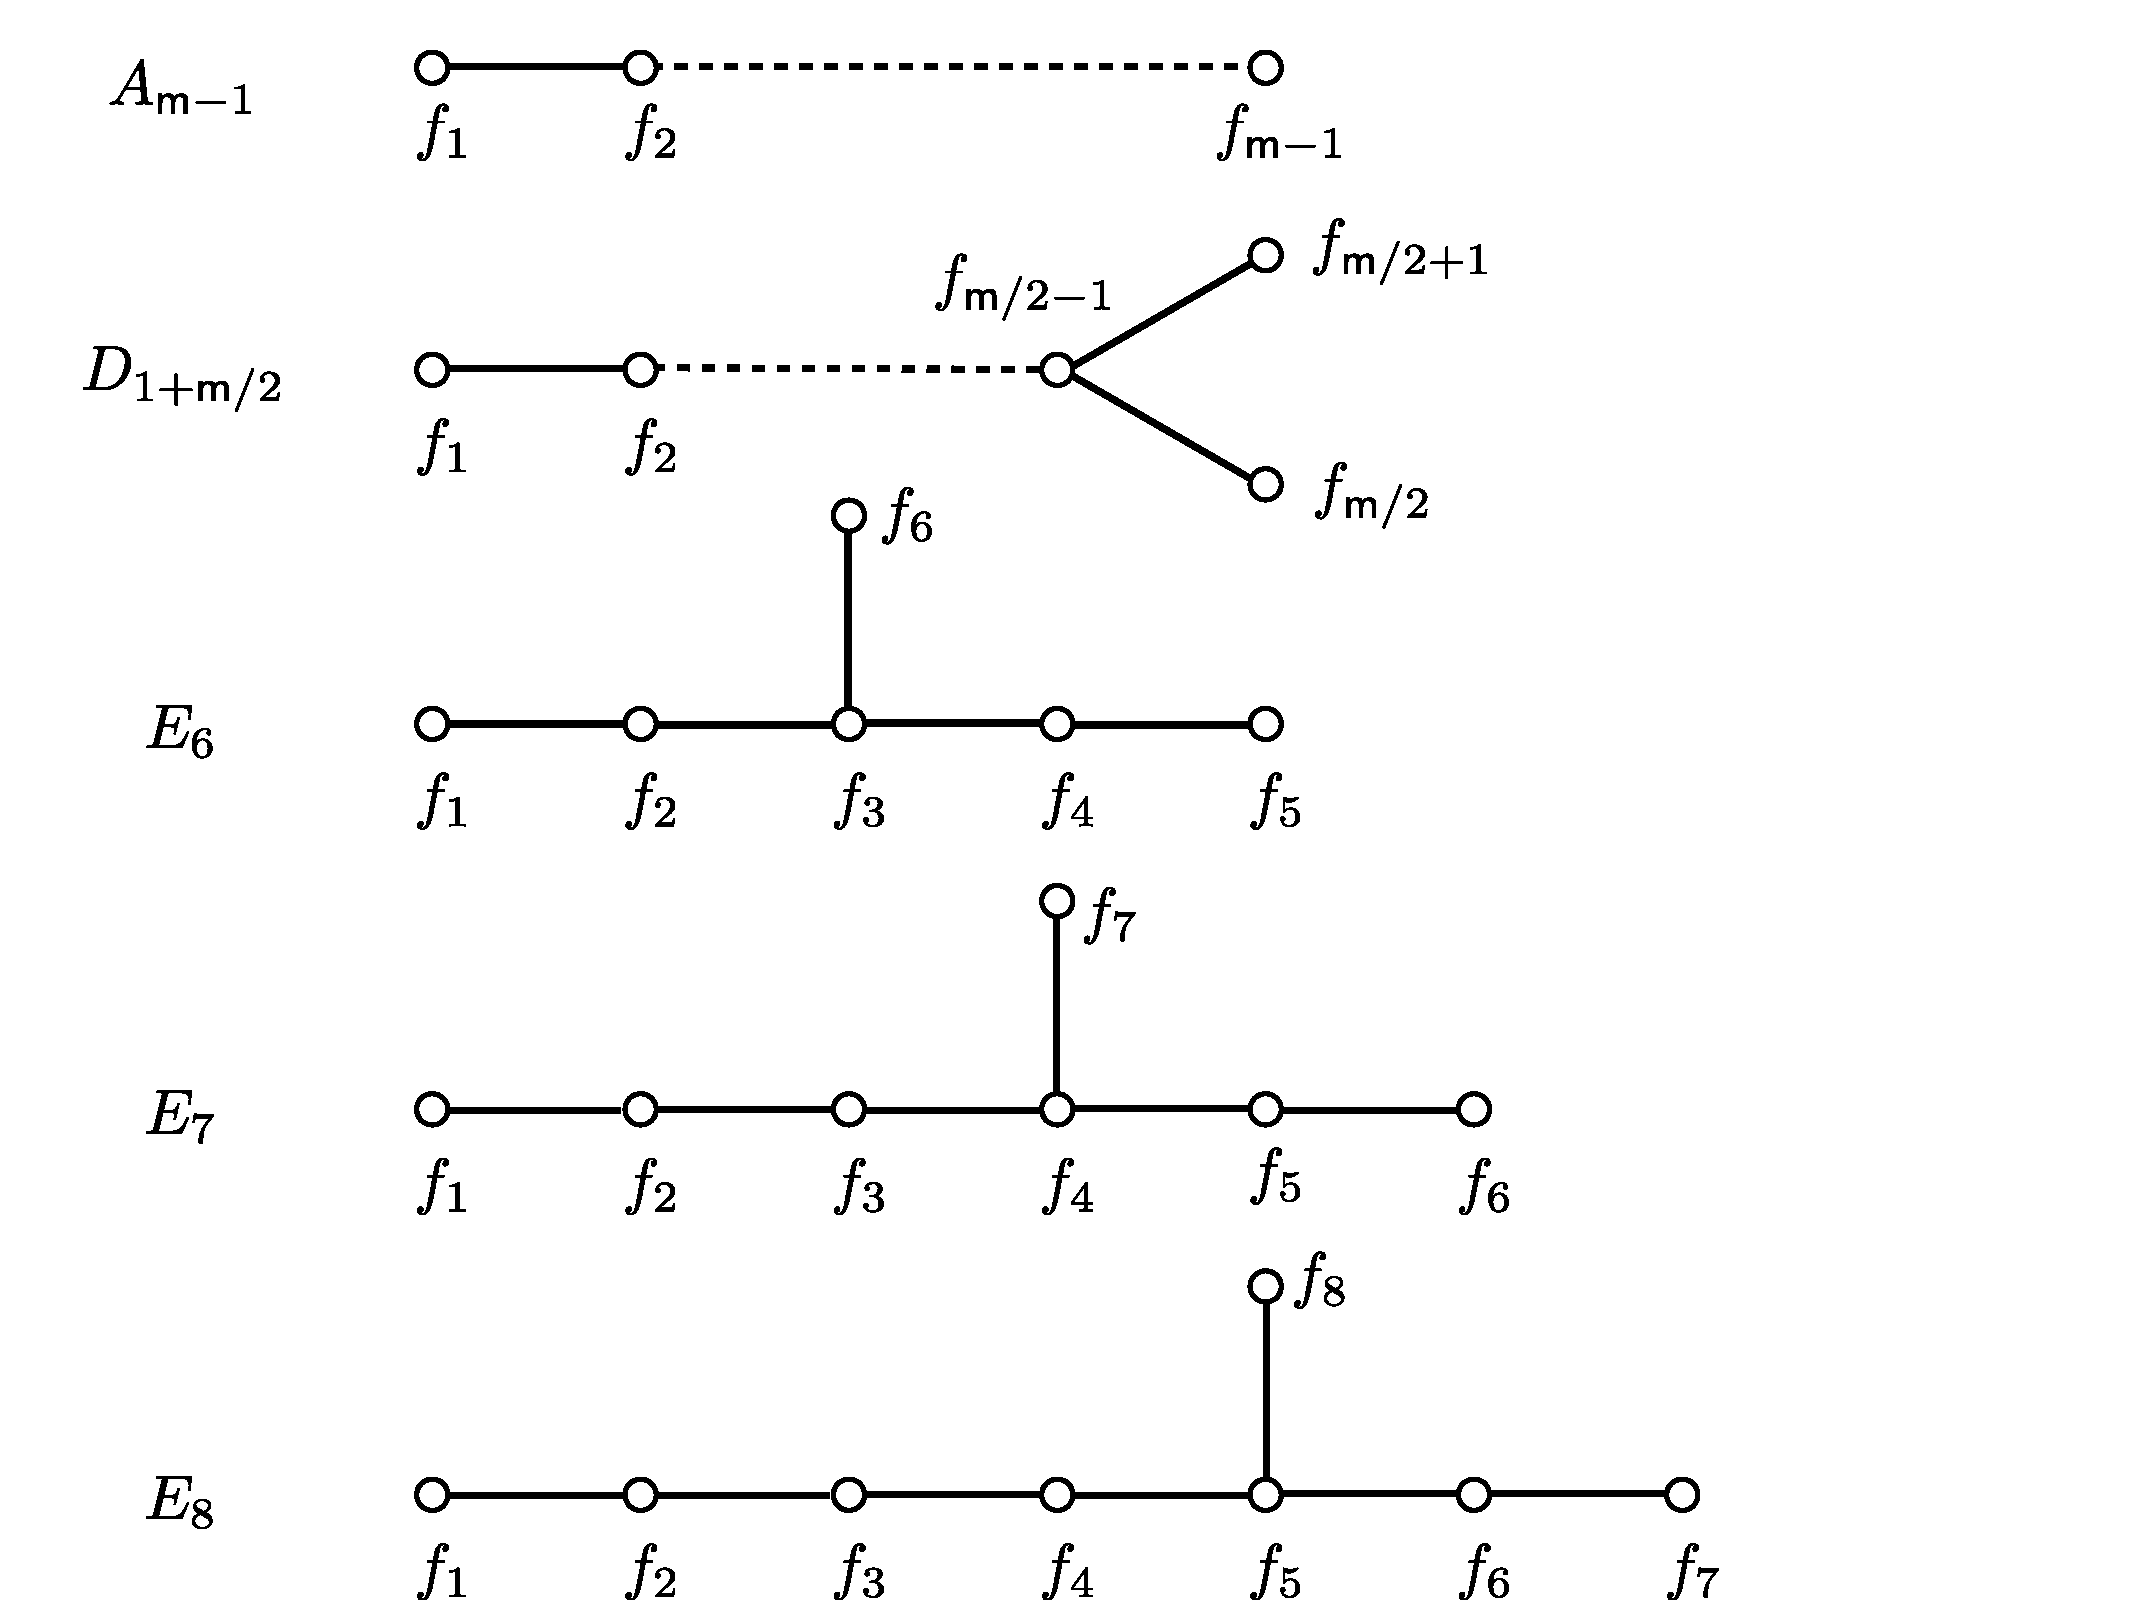
\includegraphics[width=0.62\linewidth]{figures/fig2_ade_dynkin.pdf}
    \caption{ADE Dynkin 图。（原文 p.10，图 1）}
    \label{fig:dynkin}
  \end{center}
\end{figure}

每个不可约根系统相对于给定的单根集 $\Phi$ 含有唯一的\emph{最高根} $\theta$，其分解
\begin{equation}
\theta=\sum_{i=1}^r a_i f_i
\end{equation}
使和 $\sum a_i$ 最大。于是 $X$ 的\emph{Coxeter 数}（Coxeter number）定义为
\begin{equation}
\text{Cox}(X):=1+\sum_{i=1}^ra_i~.
\end{equation}
Coxeter 数也可以用 Weyl$(X)$ 来定义。关于所有单根的反射之积 $w=r_{f_1}r_{f_2}\cdots r_{f_r}\in W^X$ 称为\emph{Coxeter 元}，它的阶等于 Coxeter 数 $m$。

% [Tutor Note: “Coxeter 元的阶等于 Coxeter 数”对不可约根系统成立，原文未给证明，标准论证见 Bourbaki《Lie Groups and Lie Algebras》第 V–VI 章。对单边根系统还有 $\text{Cox}(X)=|X|/r$（根的个数除以秩）：$E_8$ 有 240 个根、秩 8，故 Coxeter 数为 30，可用来快速验算。]

秩为 $n$ 的\emph{格} $L$ 是一个同构于加法群 $\ZZ^n$ 的自由阿贝尔群，配备对称双线性型 $\langle\cdot,\cdot\rangle$。把 $L$ 嵌入 $\RR^n$，就得到向量空间 $\RR^n$ 中一个点集的图像。对我们的用途来说，格的一些有用性质如下：
\begin{itemize}
\item \emph{正定}：双线性型在 $\RR^n$ 上诱导正定内积。
\item \emph{整}：对任意 $\lambda,\mu\in L$，有 $\langle\lambda,\mu\rangle\in\ZZ$。
\item \emph{偶}：对任意 $\lambda\in L$，有 $\langle\lambda,\lambda\rangle\in2\ZZ$。
\item \emph{幺模}：对偶格 $L^*:=\lbrace \lambda\in L \otimes_\ZZ \RR |~\langle\lambda,L\rangle\subset\ZZ\rbrace$ 同构于格本身。
\end{itemize}
$L$ 中满足 $\langle\lambda,\lambda\rangle=2$ 的所有元素 $\lambda\in L$ 称为 $L$ 的\emph{根}。

24 维的偶、幺模、正定格在月光的若干实例中扮演特殊角色，我们将在本讲义的第二部分与第三部分讨论。H. V. Niemeier 于 1973 年证明：这样的格只有 24 个互不等价的 \cite{Nie_DefQdtFrm24}。其中之一由 J. Leech 于 1967 年首次发现，称为\emph{Leech 格}，它是这 24 个格中唯一没有根向量的 \cite{Lee_SphPkgs,Con_ChrLeeLat,Lee_SphPkgHgrSpc}。其余 23 个我们称为 \emph{Niemeier 格}，它们具有非平凡的根系统。事实上，Niemeier 格的一种有用构造是把根格与适当的“粘合向量”（glue vectors）组合起来 \cite{sphere_packing}。结果表明，23 个 Niemeier 格由根系统 $X$ 唯一标记，这些 $X$ 称为 \emph{Niemeier 根系统}；它们恰是满足以下条件的 23 个单边（ADE）根系统之并 $X= \cup_i  Y_i$：1) 所有分量的 Coxeter 数相同，${\rm Cox}(Y_i)={\rm Cox}(Y_j)$；2) 总秩等于格的秩 $\sum_i {\rm rk} (Y_i)=24$。这 23 个之中的例子包括 $24A_1$、$2A_{12}$、$8E_8$ 与 $D_{16}E_8$。

% [Tutor Note: 原文举例作 $8E_8$，但 $8E_8$ 的秩为 $8\times8=64$，与同一句的条件 2（总秩 24）直接矛盾；正确的 Niemeier 根系统应为 $3E_8$（三份 $E_8$，秩 $3\times8=24$）。此处疑为原文笔误，译文照录未改，详见报告。]

对这 24 个秩 24 的偶、幺模、正定格 $N$，各定义一个有限群
\be\label{def:niemeier_grp}
G_{N} := {\rm Aut}(N)/{\rm Weyl } (N), 
\ee
其中 ${\rm Weyl } (N)$ 表示 $N$ 的根系统的 Weyl 群。特别地，当 $N=\Lambda$ 为 Leech 格时，Weyl 群 ${\rm Weyl } (\Lambda)$ 是平凡群，而 $G_{\Lambda} \cong \Co_0$ 就是 Conway 群 $\Co_0$。考虑这一群的商以及稳定各种结构的子群，可以得到许多散在群。例如，散在单群 $\Co_1$ 由对中心的商给出，$\Co_1\cong \Co_0/\{\pm1\}$；Mathieu 群 $M_{23}$ 则作为固定某个秩 2 子格的子群出现。详见 \cite{sphere_packing} 第 10 章。若改取 $N$ 为根系统 $24A_1$ 的 Niemeier 格，则有限群 $G_{N}\cong M_{24}$ 即最大的 Mathieu 群。对根系统 $12A_2$ 的 Niemeier 格，有限群为 $2.M_{12}$，即 Mathieu 群 $M_{12}$ 的非平凡扩张。这些群将在月光中（参见 \S\ref{sec:conway_moonshine}、\S\ref{sec:M24moonshine}、\S\ref{sec:umbral}）以及对其物理背景的讨论中（参见 \S\ref{chap:moonshineK3}）起重要作用。

% [Tutor Note: $G_N=\Aut(N)/\Weyl(N)$ 的取法有讲究：Weyl 群由根反射生成、总含于 $\Aut(N)$，除掉它才能留下在根系统上作用平凡的那部分对称性；Leech 格无根向量、Weyl 群平凡，故 $G_\Lambda=\Co_0$。$24A_1$ 给出 $M_{24}$、$12A_2$ 给出 $2.M_{12}$，说明同一个 Niemeier 格既决定根系统、也决定对应的月光群；Schur 乘子为 2 正是 $M_{12}$ 出现非平凡扩张的原因。]

\subsection{有限群的表示}
\label{subsec:rep}

群的结构正是描述对称性所需要的。要把它用起来，还需要群的表示这一概念。以下我们只讨论\emph{复表示}，即考虑群在复向量空间 $V$ 上的作用。更确切地说，考虑群同态 $\r:G\rightarrow\GL(V)$。我们可以把像 $\r(g)$ 看作可逆的 $n\times n$ 复矩阵。特别地有 $\rr\left(g^{-1}\right)=(\rr(g))^{-1}$。向量空间连同映射 $(V,\rr)$ 称为维数为 $n$ 的\emph{表示}。人们常把 $V$ 或 $\rr$ 单独称为表示，而隐含指整套数据。此时向量空间 $V$ 也称为 $G$-模，并说它带有 $G$-作用。若不存在两个不同元素 $g,g'\in G$ 使得 $\rho(g)=\rho(g')$，则称该 $G$-作用\emph{忠实}（相应的表示也称为忠实的）。

\myparagraph{不可约表示与对偶表示。}
给定两个表示 $(V,\rr)$ 与 $(V',\rr')$，可以直接定义它们的直和与张量积，从而得到新的表示 $V\oplus V'$ 与 $V\otimes V'$。

% [Tutor Note: 张量积 $V\otimes V'$ 的特征标等于两个特征标之积（即下文 (1.17) 的第二个等式），这是“特征标构成交换结合代数”的来源。但若群只以相差一个相位的意义作用（射影表示），$V\otimes V'$ 会把相位（2-上链）暴露出来，必须改用 Schur 乘子与中心扩张处理；本节讨论的都是“真”表示，后文月光模在中心扩张下用到的正是射影表示。]

若存在可逆 $n\times n$ 矩阵 $M$ 使得对任意 $g\in G$ 有 $M\rr'(g)=\rr(g)M$，则称两个表示 $\rr,\rr'$ 等价。表示 $(V,\rr)$ 的\emph{子表示}是一个表示 $(U,\rr')$，其中 $U$ 是子空间 $U\subset V$，在 $G$ 的作用下不变，$\rr'$ 是 $\rr$ 到 $U$ 的限制。若表示 $V$ 不含任何真子表示，则称它\emph{不可约}；若它不能写成两个（或更多）非零子表示的直和，则称它\emph{不可分解}。对有限群，这两个概念一致。若一个表示是有限多个不可约表示的直和，即它可完全分解为不可约的部分，则称它\emph{完全可约}。$G$ 的不可约表示在限制到子群 $H<G$ 时可以变为可约的，它分解为 $H$ 的不可约表示的方式由所谓的\emph{分支规则}（branching rules）给出。

所谓的 Maschke 定理说，有限群的所有（有限维）表示总是完全可约的。证明分两步。首先证明幺正表示总是完全可约的，用到的事实是：给定内积 $\lbrace\cdot,\cdot\rbrace: V\times V \to \CC$，若 $U$ 是 $V$ 的子表示，则 $U$ 在 $V$ 中的正交补也是子表示。接着证明任何表示关于群不变内积
\begin{equation}
\lbrace v,w\rbrace\coloneqq\frac{1}{| G|}\sum_{g\in G}\langle\rr(g)v,\rr(g)w\rangle,~~v,w\in V~,
\end{equation}
都是幺正的，这就完成了证明。

% [Tutor Note: 关键在第 1 步：$U$ 的 $G$-不变正交补之所以存在，靠的是内积群不变；而平均化 $\frac{1}{|G|}\sum_{g\in G}$ 要求 $|G|$ 在基域中可逆，故 Maschke 定理对特征不整除 $|G|$ 的域都成立（这里基域是 $\CC$）。若换成射影表示，平均化只能做到相差 2-上链，完全可约性要另行论证。]

我们还提到表示 $\rr$ 的\emph{对偶表示} $\rr^*$，它定义为
% [Tutor Note: 对偶表示公式里 $g^{-1}$ 与转置缺一不可：若漏掉 $g^{-1}$，则 $\rho^*(gg')$ 与 $\rho^*(g)\rho^*(g')$ 反序，得不到群同态。取 $\rho$ 幺正时 $\rho(g^{-1})=\rho(g)^{\dagger}$，于是 $\rho^*(g)=\overline{\rho(g)}$，这正是“对偶等价于复共轭”的由来；非幺正情形只能说对偶，不能与复共轭混同。]
\begin{equation}
\label{eq:dual_rep}
\rr^*(g):=\left(\rr\left(g^{-1}\right)\right)^T~,~~g\in G~, 
\end{equation}
这是对偶空间 $V^*=\End(V,\CC)$ 上的自然群作用。取 $\rho$ 为幺正表示，则 $\rho^*(g)=\overline{\rho(g)}$。换言之，对偶表示等价于复共轭表示。

\myparagraph{特征标。}
表示 $(V,\rr)$（$V$ 是 $\CC$ 上的向量空间）的\emph{特征标}（character）$\x_\rr$ 是由表示矩阵的迹定义的映射 $G\rightarrow\CC$：
\begin{equation}
\x_\rr(g)\coloneqq\tr(\rr(g))~,~~g\in G.
\end{equation}
我们也常用 $\tr_V g$ 表示这个迹。若 $\rr$ 不可约，则 $\x_\rr$ 称为不可约特征标。有限群特征标的一些性质总结如下：
\begin{itemize}

\item 特征标是\emph{类函数}，即 $\x_\rr\left(hgh^{-1}\right)=\x_\rr(g)~~\forall~g,h\in G$。这直接来自迹的循环性质。

\item 有限群的两个复表示有相同的特征标，当且仅当它们等价；这可用下面讨论的正交性证明。

\item $G$ 的特征标限制到子群 $H<G$ 上，是 $H$ 的特征标。

\item $\x_\rr\left(g^{-1}\right)=\overline{\x_\rr(g)}$，这可由以下事实看出：$\rr(g)$ 的所有本征值都是 $|g|$ 次单位根。

\item 对 $G$ 的两个表示 $\rr,\rr'$ 与 $g\in G$，有：
\begin{equation}
\x_{\rr\oplus\rr'}(g)=\x_{\rr}(g)+\x_{\rr'}(g)~,~~\x_{\rr\otimes\rr'}(g)=\x_{\rr}(g)\x_{\rr'}(g)~,~~\x_{\rr^*}(g)=\overline{\x_{\rr}(g)}~.
\end{equation}
这说明特征标构成一个交换结合代数。
\end{itemize}

\myparagraph{正交性。}
由 Schur 正交关系（例如 \cite{JonesH.F.HughF.1998Grap} 的 \S 4），幺正表示的特征标带有 Hermite 内积
\begin{equation}
\label{eq:orthog_char}
\langle\x_\rr,\x_{\rr'}\rangle=\frac{1}{|G|}\sum_{g\in G}\x_\rr(g)\overline{\x_{\rr'}(g)}~.
\end{equation}
当 $\rho$ 与 $\rho'$ 是不可约表示时，可以证明：若两个不可约表示等价，则 $\langle\x_\rr,\x_{\rr'}\rangle=1$，否则为零。于是，不可约表示的特征标是类函数空间中的正交归一向量。事实上可以证明它们张成这个空间，由此可得一个重要事实：不等价不可约表示的个数等于共轭类的个数（例如见 \cite{HamermeshMorton1962Gtai} 的 \S 3-7）。此外还可以证明另一个正交归一性质，
\begin{equation}
\sum_{\rr}^{}\x_{\rr}(g)~\overline{\x_{\rr}(h)}=\left\lbrace\begin{matrix} |C_G(g)|, & h\in [g] \\ 0, & \text{其他情形} \end{matrix}\right.~,
\end{equation}
其中求和遍历不等价的不可约表示，$|C_G(g)|$ 表示 $g\in G$ 的中心化子的阶，它等于群的阶除以共轭类 $[g]$ 中元素的个数。

% [Tutor Note: 第一正交关系里的 $1/|G|$ 归一化与复共轭缺一不可；对幺正表示有 $\overline{\chi_{\rho'}(g)}=\chi_{\rho'}(g^{-1})$，故也可写成 $\frac{1}{|G|}\sum_g\chi_\rho(g)\chi_{\rho'}(g^{-1})$。第二正交关系右端是中心化子阶 $|C_G(g)|$ 而非 $|G|$，且只在 $h\in[g]$ 时非零，利用 $|G|=|C_G(g)|\cdot|[g]|$ 可与第一式互相印证。]

% [Tutor Note: “它们张成类函数空间”是特征标理论的核心一步，作者略去了证明；标准做法是对任意类函数 $f$ 比较 $\sum_\rho\langle f,\chi_\rho\rangle\chi_\rho$ 与 $f$，或直接引用有限群表示论中 Schur 正交关系的完备性（参见 \cite{HamermeshMorton1962Gtai} 的 \S 3-7）。由“正交归一 + 张成”立刻得到不可约表示数等于共轭类数，这正是特征标表为方阵的原因。]

\myparagraph{特征标表。}
我们已经提到，有限群 $G$ 的不可约表示个数等于 $G$ 的共轭类个数。我们可以把 $G$ 的所有特征标汇总为\emph{特征标表}，它是一个 $\Cl(G)\times\Cl(G)$ 的方表，行标记不同的不可约表示，列标记不同的共轭类。换言之，特征标表的 $(i,j)$ 元是第 $i$ 个不可约表示的特征标 $\x_i(g)$ 在第 $j$ 个共轭类中任一 $g$ 处的取值。作为一个例子，交错群 $\mathcal{A}_6$ 的特征标表见表 \ref{tbl:char_table_ex}。
\begin{table}
\centering
\begin{tabular}{|c|c|c|c|c|c|c|c|c|}
\hline    &    & 1A & 2A & 3A & 3B & 4A & 5A & 5B \\ \hline \hline
          & 2P & 1A & 1A & 3A & 3B & 2A & 5B & 5A \\ \hline
          & 3P & 1A & 2A & 1A & 1A & 4A & 5B & 5A \\ \hline
          & 5P & 1A & 2A & 3A & 3B & 4A & 1A & 1A \\ \hline  \hline
$\x_1$    &    &  1 &  1 &  1 &  1 & 1 & 1 & 1 \\ \hline
$\x_2$    &    &  5 &  1 &  2 & -1 &-1 & 0 & 0 \\ \hline
$\x_3$    &    &  5 &  1 & -1 &  2 &-1 & 0 & 0 \\ \hline
$\x_4$    &    &  8 &  0 & -1 & -1 & 0 &$A$& $^*A$ \\ \hline
$\x_5$    &    &  8 &  0 & -1 & -1 & 0 &$^*A$& $A$ \\ \hline
$\x_6$    &    &  9 &  1 &  0 &  0 & 1 &-1 &-1 \\ \hline
$\x_7$    &    & 10 & -2 &  1 &  1 & 0 & 0 & 0 \\ \hline
\end{tabular}
\caption{$\mathcal{A}_6$ 的特征标表，其中 $A=\frac{1-\sqrt{5}}{2}$、$^*A=\frac{1+\sqrt{5}}{2}$。（原文 p.14）}
\label{tbl:char_table_ex}
\end{table}
注意上表还包含额外信息，即所谓的幂映射（power map）。以 $s$P 开头的那一行给出共轭类 $[g^s]$。

\myparagraph{超模。}
超空间（$\ZZ_2$-分次向量空间）上的 $G$-模称为 $G$-\emph{超模}。具体地说，若 $V$ 是 $G$-超模，则它具有结构
\be\label{def:supermodule}
V  = V_{\underline{0}} \oplus V_{\underline{1}}
\ee
其中 $V_{\underline{0}}$ 与 $V_{\underline{1}}$ 都是 $G$-模。我们有时把 $V$ 称为 $G$ 的\emph{虚表示}。\emph{超迹} ${\str}$ 定义为其在奇子空间上带负号作用：${\str}_V g := \tr_{V_{\underline{0}}} g-\tr_{V_{\underline{1}}}g$。

\myparagraph{轮换型与 frame shape。}
顾名思义，群 $G$ 的 $N$ 维\emph{置换表示} $\rr_p$ 以 $N\times N$ 置换矩阵为表示矩阵（除每行每列恰有一个元素为 1 外全为零）。给定这样的表示，其每个共轭类可以联系一个\emph{轮换型}（cycle shape），它编码该类元素所对应的置换轮换的个数与类型。轮换型的一般形式为
\begin{equation}
n_1^{\ell_1}n_2^{\ell_2}\cdots n_r^{\ell_r}~,~~\sum_{s=1}^r\ell_s n_s=N~, 
\end{equation}
其中 $n_s, \ell_s$ 都是正整数，$n$ 表示一个\emph{$n$-轮换}，即 $n$ 个元素的置换。指数 $\ell_s$ 计数 $n_s$-轮换的个数。显然，阶为 $k$ 的元素只能有大小 $n_s$ 整除 $k$ 的轮换。注意，轮换型可以直接从特征标表（包括幂映射）读出。

更一般地，给定任意表示 $\rho$，只要 $\rho$ 的所有特征标都是有理数，我们就可以定义 $g\in G$ 的\emph{frame shape}。有理性保证：若 $\lambda$ 是 $g$ 的本征值，则当 $k$ 与 $|g|$ 互素时 $\lambda^k$ 也是本征值 \cite{MasonGeoffrey1984Farc}。把 $g$ 的本征值记为 $\l_1, \l_2,\dots ,\l_N$，则存在正整数 $i_1,i_2,\dots,i_s$ 与基数相同的非零整数 $\ell_1,\ell_2,\dots,\ell_s$，使得
\begin{equation}
\det(\mathbf{1}-t\rho(g))=\prod_{i=1}^N(1-t\lambda_i)=\prod_{r=1}^s(1-t^{i_r})^{\ell_r}~.
\end{equation}
显然必须有 $\sum_{s=1}^r\ell_s i_s=N$，我们称
$
i_1^{\ell_1}i_2^{\ell_2}\cdots i_r^{\ell_r}
$
为共轭类 $[g]$ 在表示 $\rho$ 下的 frame shape。

% [Tutor Note: 原文上方公式的指标混用：前面声明的是 $i_1,\dots,i_s$ 共 $s$ 个，但乘积写成 $\prod_{r=1}^{s}$，frame shape 末尾又写成 $i_r^{\ell_r}$，同一段后面的求和也用 $\sum_{s=1}^r$。按上下文应统一以 $s$ 为指标；译文照录原文，未改。]


% ==================== 内联自 chapters/ch02_modular.tex ====================
% ===================================================================
%  第 2 节 模对象 原文：TASI10.tex 第 607--1050 行（PDF p.15--25）
% ===================================================================
\section{模对象}
\label{sec:modular}

\begin{keytakeaways}
  \item 模形式是上半平面上满足 $f(\t)=(c\t+d)^{-k}f\big(\frac{a\t+b}{c\t+d}\big)$ 的全纯函数；$\SL_2(\ZZ)$ 的模形式环由 $E_4$、$E_6$ 自由生成，权零模函数域则由主模 $J=q^{-1}+O(q)$ 生成，见式 (2.3)--(2.5)。
  \item theta 函数、Dedekind eta 函数与 Eisenstein 级数是基本构件；$\eta(\t)=q^{1/24}\prod(1-q^n)$ 是带非平凡乘子的权 $1/2$ 形式，而 $\eta^{24}=\Delta$ 才是权 12 的尖形式，见式 (2.19)--(2.21)。
  \item 权 $k$、指标 $m$ 的 Jacobi 形式是 $\HH\times\CC$ 上的椭圆形式，其模变换同时重标度 $\t$ 与 $z$，并带指数因子 $\ex(-cmz^2/(c\t+d))$；它等价于向量值模形式 $h=(h_r)$ 的 theta 分解，见式 (2.22)--(2.27)。
  \item 弱 Jacobi 形式的环由 $\phi_{0,1}$ 与 $\phi_{-2,1}$ 在 $\SL_2(\ZZ)$ 的模形式环上自由生成，且 $2\phi_{0,1}$ 就是 K3 的椭圆亏格，见式 (2.31)、(2.32)。
  \item 模拟模形式 $h$ 的模变换缺陷由权 $2-w$ 的影子 $g$ 补偿：完备化 $\hat h=h+g^\ast$ 是权 $w$ 的调和 Maass 形式，$g^\ast$ 由不完全 gamma 函数给出的 Eichler 积分确定，见式 (2.34)--(2.36)。
  \item 本影月光的权 $1/2$ 模拟模形式 $H=H^{24A_1}$ 以 $24\eta^3$ 为影子；其 $H/2$ 的 Fourier 系数 45、231、770、2277、5796 是 $M_{24}$ 不可约表示的维数，见式 (2.42)--(2.45)。
\end{keytakeaways}

本章简要介绍模形式的概念及其若干推广，包括模拟模形式（mock modular form）、Jacobi 形式（Jacobi form）与模拟 Jacobi 形式。

\subsection{模形式}
\label{subsec:modular_forms}

模形式的标准参考文献之一是 \cite{2008T1om}，本章部分内容依此展开。众所周知，$\SL_2(\RR)$ 通过分式线性（Möbius）变换作用在上半平面 $\HH:=\{\t\in \CC\lvert~ \Im(\t) > 0\}$ 上：
\be
\gamma = \begin{pmatrix} a &b \\ c&d\end{pmatrix} : \HH \to \HH~,~~ \t \mapsto \gamma\t := {a\t+b\over c\t+d}~. 
\ee

% [Tutor Note: $\HH$ 上的 Möbius 作用保持 $\Im\t>0$，因为 $d\gamma\t/d\t=(c\t+d)^{-2}$ 的辐角变化不改变 $\t$ 的虚部符号；又 $\gamma$ 与 $-\gamma$ 给出同一变换，故真正起作用的是 $\PSL_2(\RR)$。式 (2.1) 的约定是“矩阵左乘作用在 $\t$ 上”，下文所有权重因子 $(c\t+d)^{-k}$ 都以这一约定为准。]

在定义模形式时，我们考虑 $\SL_2(\RR)$ 的离散子群，其中重要的例子是模群 $\SL_2(\ZZ)$。它由
\be
T = \bem 1& 1\\ 0&1\eem~~{\rm and}~~ S = \bem 0& 1\\ -1&0 \eem
\ee
生成，满足 $(ST)^3=1$ 与 $S^2=-1$。我们也常使用 $\PSL_2(\ZZ)\cong \SL_2(\ZZ)/\{\pm 1\}$，它同时也是环面的映射类群（参看 \S\ref{sec:CFT}）。
我们还会经常考虑把 {\em 尖点}（cusps）$\{i\infty\} \cup \QQ$ 添加上去所得的扩充上半平面；$\SL_2(\ZZ)$ 在尖点集上传递地作用，这一点从 $\gamma\infty = {a\over c}$ 即可看出。

% [Tutor Note: 这里的传递性是初等数论：给定互素的 $a,c$，由 Bezout 定理可取 $b,d$ 使 $ad-bc=1$，故 $\gamma\infty=a/c$ 取遍所有有理数，再加上 $c=0$ 给出的 $i\infty$。作者用“one can see from”一带而过，读者需自补这一步；注意 $\gamma\infty$ 只依赖 $\gamma$ 的第一列。]

我们从模群 $\SL_2(\Z)$ 上的权零模形式开始定义：它就是上半平面上在 $\SL_2(\Z)$ 作用下不变的全纯函数，
\be \label{def0_mmf}
f(\t)  =  f(\gamma\t)\quad \forall~ \gamma \in \SL_2(\Z).
\ee
特别地，当 $\t$ 趋近 $\HH$ 在尖点 $\{i\infty\} \cup \QQ$ 处的边界时，$f$ 必须保持全纯。但这一要求过强：基本的复分析告诉我们，这样的函数只有常数。

% [Tutor Note: 作者省略的论证是：紧化后的 $\SL_2(\Z)\backslash\widehat\HH$ 是紧 Riemann 面，$f$ 在其上全纯，由最大模原理必为常数。“在尖点全纯”正是 $f$ 能延拓到该紧 Riemann 面上的条件；若只要求 $\HH$ 内全纯，$q^{-1}$ 型极点就允许出现，这正是下一条“弱全纯”推广的动机。]

因此，我们希望在以下几个方向上进一步推广上述定义：
\begin{enumerate}
\item {\it 解析性}：允许函数在尖点附近有指数增长。这样的函数称为 {\it 弱全纯模形式}（weakly holomorphic modular forms）。
\item {\it 权重}：允许变换规则中出现一个标度因子，见 (\ref{def1_mmf})。
\item {\it 其他群}：把变换性质 (\ref{def0_mmf}) 中的 $\SL_2(\Z)$ 换成一般的 $\Gamma < \SL_2(\RR)$。
\item {\it 乘子}：修改变换规则 (\ref{def0_mmf})，允许一个非平凡特征标 $\psi : \SL_2(\Z) \to \CC^\ast$，见 \eqref{def1_mmf}。
\item {\it 向量值}：把 $f: \HH \to \CC$ 换成有 $n$ 个分量的向量值函数 $f: \HH \to \CC^n$。
\end{enumerate}

当然，上述推广可以组合使用。例如，可以考虑 $\SL_2(\RR)$ 的某个子群 $\Gamma$ 上带乘子的向量值模形式。显然，在向量值情形，特征标 $\psi$ 不再是相位，而是一个矩阵。
这些概念也并不完全独立。例如，$\SL_2(\Z)$ 的向量值模形式的一个分量，可以看作 $\SL_2(\Z)$ 某个子群上的（单值）模形式，反之亦然。

我们先从第一种推广入手，引入 {\it 模函数}（modular functions）的概念。若 $f:\HH\to \CC$ 在 $\HH$ 内亚纯、满足变换规则 (\ref{def0_mmf})，并且对某个有限的 ${m> -\infty}$ 按 $e^{2\pi i \t m}$ 增长，则称 $f$ 为模函数。

% [Tutor Note: “按 $e^{2\pi i\t m}$ 增长”是“在尖点处至多指数增长”的精确化：存在有限的 $m$ 使 $f(\t)=O(q^m)$（$q=\ex(\t)$）。$m>-\infty$ 只强调 $m$ 有限，允许 $m<0$，即允许尖点处的极点；若对任意 $m$ 都成立，$\SL_2(\Z)$ 不变性会迫使 $f$ 为常数。]

事实上，模函数构成一个单生成的函数域，生成元称为 {\it 主模}（Hauptmodul，亦称 principal modulus）。这是因为，添上有限多个点之后，基本域 $\SL_2(\Z)\backslash \HH$ 是亏格零的 Riemann 面。

% [Tutor Note: 亏格零的紧 Riemann 面同构于 $\widehat\CC$，其亚纯函数域是单变量有理函数域 $\CC(J)$，这就是“单生成”的来源，也是 Hauptmodul 一名的由来。原文此处称“This is because”，略去了这个标准事实：$\SL_2(\Z)\backslash\widehat\HH\cong\mathbb{P}^1$，其上的亚纯函数恰为 $J$ 的有理函数。]

把加上尖点后的上半平面记为 $\widehat \HH = \HH \cup\{i\infty\} \cup \QQ$，则 Hauptmodul 给出两个球面 $\SL_2(\Z)\backslash \widehat\HH$ 与 $\widehat \CC$ 之间的同构。显然，这样的 Hauptmodul 在 Möbius 变换（即球面上三个点的选取）之下唯一。因此，具有展开
\be
J(\t) = q^{-1} + O(q)
\ee
的 Hauptmodul 唯一。这里及下文记 $q:= \ex(\t)$，其中 $\ex(x):=e^{2\pi i x}$，$x\in \CC$。

% [Tutor Note: 归一化条件 $q^{-1}+O(q)$ 固定了球面自同构的三个自由度：$J(i\infty)=\infty$、以 $q$ 为局部坐标时在 $q=0$ 处留数为 1 的单极点、常数项为 0。换一套归一化得到的是 $J$ 的 Möbius 变换，函数域不变但数值不同；月光中比较不同群的主模时，务必先核对归一化。]

用 Eisenstein 级数与 Dedekind eta 函数（参看 \eq{def:E4E6} 与 \eq{def:dedeta}），$J$ 函数可写成
\be\label{eq:def_J}
J(\tau) = j(\tau) -744 =  {E_4^3(\t)\over  \eta^{24}(\t)}-744. 
\ee

% [Tutor Note: 注意 $j:=E_4^3/\Delta$（$\Delta=\eta^{24}$）的 $q$ 展开是 $q^{-1}+744+196884q+\dots$，故必须减去 744 才满足 (2.4) 的归一化。系数 196884 是魔群最小忠实表示维数 196883 与平凡表示维数之和，即魔群月光猜想的起点；用 $j$ 而非 $J$ 会使所有 McKay–Thompson 系数整体平移。]

一般地，只要 $\Gamma\backslash \widehat\HH$ 亏格零，就可以把 $\Gamma\leq \SL_2(\RR)$ 的模函数域的生成元定义为主模。这些 Hauptmodul 在月光中起重要作用。

% [Tutor Note: 魔群月光的核心结论正是：对魔群 $\mathbb{M}$ 的每个元素 $g$，其 McKay–Thompson 级数 $T_g$ 都是某个亏格零群 $\Gamma_g<\SL_2(\RR)$ 的 Hauptmodul（Conway–Norton 猜想，Borcherds 1992 年证明）。故本段“Hauptmodul 在月光中起重要作用”并非泛泛之谈：月光关系就是“共轭类的级数 = 亏格零群的主模”。]

除了上述定义，模函数还有三种等价看法。第一，由 (\ref{def0_mmf})，可以把 $f$ 看作从适当紧化的基本域 $\SL_2(\Z) \backslash \HH$ 到 Riemann 球面 $\widehat\CC=\CC\cup \{\infty\}$ 的函数。第二，由 $\SL_2(\Z)$ 与秩二格的关系，可以为每个 $\t$ 配上复格 $\Lambda_\t :=1\cdot \ZZ+\t\cdot \ZZ$，并把 $f$ 看作给每个这样的格 $\Lambda_\t$ 指定复数 $f(\t)$ 的函数；它还在格的重新标度下不变。第三种看法在模形式与二维共形场论的联系中起重要作用，它来自把 $\SL_2(\Z)\backslash \HH$ 解释为亏格一 Riemann 面的复结构模空间。
这一点很容易从以下事实看出：环面可描述为复平面模去一个秩二格，因此在相差一个标度之下由 $\CC/\Lambda_\t$ 给出，其中 $\t\in \HH$。
于是模函数可以理解为给每个环面指定一个只依赖其复结构模 $\t$ 的复数。
在这个语境下，群 $\PSL_2(\Z) := \SL_2(\Z)/\{{\mathds{1}},-{\mathds{1}}\}$ 扮演环面的映射类群（参看 \S\ref{sec:CFT}），其中中心子群 $\Z_2=\{{\mathds{1}},-{\mathds{1}}\}$ 在 $\HH$ 上平凡地作用。

% [Tutor Note: 第三种看法是本章与物理的接口：二维 CFT 的配分函数定义在环面上，环面的复结构由 $\t$ 刻画，而 $\t$ 与 $\gamma\t$ 给出同构的环面，所以“模不变性”就是配分函数为 $\t$ 的模函数。$\PSL_2(\Z)$ 作为映射类群作用在环面上，这正是第 \ref{sec:CFT} 节讨论的模群来源，也解释了为何月光级数的 $q$ 展开系数可解释为态计数。]

接下来转向第二种推广，引入模群 $\SL_2(\Z)$ 上一般权重 $k$ 的模形式。它们是 $\HH$ 上的全纯函数，在 $\SL_2(\Z)$ 作用下按
\be\label{def1_mmf}
f(\t)  =  ( c\t+d)^{-k} f\left(\frac{a\t+b}{c\t+d}\right)\quad \forall~\bem a& b\\ c&d\eem \in \SL_2(\Z)~.
\ee
变换。

% [Tutor Note: 权重约定是本章最易错处：$(c\t+d)^{-k}$ 中的 $\t$ 是变换前的 $\t$，而 $f$ 的自变量已是 $\gamma\t$。若把因子写成 $(c\,\gamma\t+d)^{-k}$，得到的是右作用约定（相当于把 $\gamma$ 换成 $\gamma^{-1}$），与 (2.6) 差一个相位；若把 $(c\t+d)^{+k}$ 抄成正幂则直接把权 $k$ 变成 $-k$。另注意 $k$ 为奇数时 $-\mathds{1}$ 给出因子 $(-1)^{-k}=-1$，故奇权形式在 $\SL_2(\Z)$ 上必须带乘子系统或改用 metaplectic 双覆盖，见下一条脚注。]

从格的观点看，我们考虑与格 $\Lambda$ 相关联的复函数 $f$，要求它在格的重新标度 $\Lambda \mapsto \lambda \Lambda$（$\lambda\in\CC$）下按 $f\mapsto \lambda^{-k}f$ 变化。
我们将考虑整数与半整数权重 $k$。\footnote{显然，$k$ 为半整数时需特别小心。严格地说，应当使用 $\SL_2(\Z)$ 的 metaplectic 双覆盖。不过，这里的微妙之处不会给我们造成困难，故不在此讨论；细节请参看 \cite{MR1773561}。}

有了这个定义，即便仍要求在尖点处全纯，也开始出现非平凡的例子。例如，下述 Eisenstein 级数
\begin{gather}\label{def:E4E6}
\begin{split}
E_4(\t) &= 1+240 \sum_{n=1}^\infty \frac{n^3 q^n}{1-q^n}= 1+240 \,q +2160\,q^2+\dots \\ 
E_6(\t) &= 1-504 \sum_{n=1}^\infty \frac{n^5 q^n}{1-q^n}= 1-504 \,q -16632\,q^2+\dots
\end{split}
\end{gather}
分别是权 4 与权 6 的模形式。

% [Tutor Note: Eisenstein 级数的归一化极易记错：式 (2.7) 采用“常数项为 1”的归一化，即 $E_4=1+240\,q+\dots$、$E_6=1-504\,q+\dots$，于是 $E_4^3-E_6^2=1728\,\Delta$。若改用 $G_{2k}=\sum_{(m,n)\neq(0,0)}(m+n\t)^{-2k}$ 的约定，则 $E_{2k}=G_{2k}/(2\zeta(2k))$，常数项仍为 1，但每个系数都带 $\zeta$ 因子；比较文献公式前先确认归一化，否则 240、504 这类系数会整体错位。]

但这个定义仍有些过强，因为 Eisenstein 级数就只有这两个：$\SL_2(\Z)$ 上的模形式环由 $E_4$ 与 $E_6$ 自由生成。也就是说，任何整权 $k$ 的模形式都可以（唯一地）写成单项式 $E_4^\a E_6^\b$ 的和，其中 $k=4\a+6\b$。记群 $\Gamma$ 的权 $k$ 模形式空间为 $M_k(\Gamma)$。在模形式中，所谓的尖形式往往特别受关注。
若权 $k$ 的模形式 $f$ 使得 $y^{k/2} f(x+i y)$ 在 $y\to \infty$ 时有界，则称 $f$ 为尖形式（cusp form）。这个条件保证 $f$ 在每个尖点处的 Fourier 展开中常数项为零。

% [Tutor Note: “$E_4$、$E_6$ 自由生成”有前提：$k=4\a+6\b$ 需有非负整数解，$k=2$ 时 $M_2=0$（$E_2$ 不是模形式），$k$ 为大于等于 4 的偶数时成立。尖形式定义中 $y^{k/2}f$ 有界等价于每个尖点的常数项为零，因为 $y^{k/2}|q^n|$ 在 $y\to\infty$ 时衰减当且仅当 $n>0$；故该条件恰好排除 $n=0$ 项。]

在第三种类型的推广中，我们常遇到由下述同余条件定义的 $\SL_2(\ZZ)$ 子群。对正整数 $N$，定义
\be\label{def:cong_subgr}
\Gamma_0(N) := \left\{ \bem a& b \\ c&d \eem \in \SL_2(\ZZ) ~\mid c\equiv 0 \xmod{N}  \right\}~. 
\ee
下面用一些例子说明上述推广。

% [Tutor Note: $\Gamma_0(N)$ 是“上三角模 $N$”的子群：它包含 $T$，一般不含 $S$，故其模形式只在 $\Gamma_0(N)$ 下不变。它的指标是 $[\SL_2(\Z):\Gamma_0(N)]=N\prod_{p\mid N}(1+1/p)$，对应模曲线 $X_0(N)$ 的亏格决定是否存在主模——月光中“亏格零群”的限制正是由此而来。]

先考虑 Jacobi theta 函数。考虑一维格，其双线性型为 $\langle x,x \rangle =x^2$。相应的 theta 函数为
\be
\theta_3(\tau)  = \sum_{n\in \Z} q^{n^2/2} \, . 
\ee
这个简单函数可以用无穷乘积表示，
\be
\theta_3(\tau)  = \sum_{n\in \Z} q^{n^2/2} = \prod_{n=1}^\infty (1-q^n)(1+q^{n-1/2})^2~, 
\ee
并且具有漂亮的模性质。
为描述这些模性质，最自然的做法是再引入两个 theta 函数，
\begin{equation}
\begin{split}
\theta_2(\tau) & = \sum_{n+{1\over 2}\in \Z} q^{n^2/2} =2q^{1/8} \prod_{n=1}^\infty (1-q^n)(1+q^{n})^2~, \\
\theta_4(\tau) & = \sum_{n\in \Z} (-1)^n q^{n^2/2} = \prod_{n=1}^\infty (1-q^n)(1-q^{n-1/2})^2~.
\end{split}
\end{equation}
它们恰好是 $\SL_2(\Z)$ 的一个向量值模形式的三个分量
\be\label{eqn:transf_theta}
\Theta(\t) := \bem  \theta_2(\tau) \\ \theta_3(\tau) \\ \theta_4(\tau)  \eem,~~   \Theta(\t) = \sqrt{i\over \t} {\cal S}\,   \Theta\left(\!-\frac{1}{\t}\right)  = {\cal T} \,\Theta(\t+1)\, ,
\ee
其中
\be
{\cal S} = \bem  0&0&1\\ 0&1&0 \\ 1&0&0 \eem , ~~{\cal T} = \bem  e(-\tfrac{1}{8})&0&0\\ 0&0&1 \\ 0&1&0 \eem  . 
\ee

% [Tutor Note: (2.12) 把 $\sqrt{i/\t}$ 写在 $\Theta(-1/\tau)$ 一侧，等价写法是 $\Theta(-1/\t)=\sqrt{\t/i}\,{\cal S}^{-1}\Theta(\t)$。${\cal T}$ 中的相位 $\ex(-1/8)$ 来自 $\theta_2$ 的 $q^{1/8}$：$\theta_2(\t+1)=\ex(1/8)\theta_2(\t)$，而 (2.12) 写成 $\Theta(\t)={\cal T}\,\Theta(\t+1)$，故矩阵元取 $\ex(-1/8)$；$\theta_3\leftrightarrow\theta_4$ 的交换给出 ${\cal T}$ 中的置换块。半整数权的相位分支（$\sqrt{i/\t}$ 的符号）必须与这一写法方向一致，抄写时最易把相位取反。]

为了说明向量值模形式与同余子群上模形式的关系，考虑 $\theta(\tau) := \theta_3(2\tau)$。它按如下方式成为 $\Gamma_0(4)$ 上带非平凡乘子的权 $1/2$ 模形式：
\be
\theta(\tau)  = \left(\frac{c}{d}\right) \epsilon_d ~ (c\t+d)^{-\frac{1}{2}} ~  \theta(\gamma\tau)  
\ee
对所有 $\gamma\in\Gamma_0(4)$ 成立，其中
\[ 
\epsilon_d:=\left\lbrace\begin{array}{rl} 1~, & d\equiv1\bmod4 \\ i~, & d\equiv3\bmod4 \end{array} \right.
\]
上面用到的 Legendre 符号定义为\footnote{若存在 $x\in\mathbb{Z}$ 使 $x^2\equiv\kappa\bmod\lambda$，则称 $\kappa$ 为模 $\lambda$ 的二次剩余。}
\[
\left(\frac{\kappa}{\lambda}\right):=\left\lbrace\begin{array}{rl} +1~, & \text{若~}~\kappa\neq0\bmod\lambda\text{ 且 $\kappa$ 为模 $\lambda$ 的二次剩余} \\ -1~, & \text{若~}~\kappa\neq0\bmod\lambda\text{ 且 $\kappa$ 不是模 $\lambda$ 的二次剩余} \\ 0~, & \text{若~}~\kappa\equiv0\bmod\lambda\end{array}\right.~.
\]

% [Tutor Note: (2.14) 是半整数权乘子的样板：$(c/d)$ 是二次剩余符号，$\epsilon_d$ 由 $d\bmod 4$ 取 $1$ 或 $i$。它只对 $\Gamma_0(4)$ 成立，对全 $\SL_2(\Z)$ 并不成立；这正是上文“向量值形式的分量可视为子群上的单值形式”的具体例子。还须注意符号 $(\kappa/\lambda)$ 中 $c$ 在上、$d$ 在下，与通常把模数写在下面的 Legendre 符号习惯相反，抄写时勿颠倒。]

后面我们会看到，这些 theta 函数可以自然地看作两变量 Jacobi theta 函数在 $z=0$ 处的特殊化；后者既可以定义为无穷和，也可以定义为无穷乘积：

% [Tutor Note: 从 (2.15) 起隐含约定 $y:=\ex(z)=e^{2\pi i z}$，而原文未再明说；若把 $y$ 当作一般变量，就读不懂 theta 级数的模变换。$z=0$ 对应 $y=1$，这就是上一句“特殊化”的确切含义。]

\begin{equation}
\begin{split}
\theta_1(\tau,z) & = -i \sum_{n+{1\over 2}\in \Z} (-1)^{n-{1\over 2}} y^n q^{n^2/2} \\
&=-iq^{1/8} (y^{1/2}-y^{-1/2})\prod_{n=1}^\infty (1-q^n)(1-yq^{n})(1-y^{-1}q^{n})\, ,\\
\theta_2(\tau,z) & = \sum_{n+{1\over 2}\in \Z} y^n q^{n^2/2} \\
&=(y^{1/2}+y^{-1/2})q^{1/8} \prod_{n=1}^\infty (1-q^n)(1+yq^{n})(1+y^{-1}q^{n}) \, ,\\
 \theta_3(\tau,z)  &= \sum_{n\in \Z} y^n q^{n^2/2} = \prod_{n=1}^\infty (1-q^n)(1+yq^{n-1/2})(1+y^{-1}q^{n-1/2})\, , \\
\theta_4(\tau,z) 
&= \sum_{n\in \Z} (-1)^n y^n q^{n^2/2} = \prod_{n=1}^\infty (1-q^n)(1-yq^{n-1/2})(1-y^{-1}q^{n-1/2})~.
\end{split}
\end{equation}
它们按如下方式变换。
令
\be
\Theta(\t,z): = \bem  \theta_1(\tau,z) \\ \theta_2(\tau,z) \\ \theta_3(\tau,z) \\ \theta_4(\tau,z) \eem~, 
\ee
则（参看 \S\ref{subsec:shjacobiforms}）
\be
\Theta(\t,z) =  \sqrt{i\over \t} \, e\big(-\frac{z^2}{2\t}\big) \, {\cal S}'\,   \Theta\big(-{1\over \t},{z\over\t}\big)  ={\cal T}' \,\Theta(\t+1,z)\, ,
\ee
其中
\be
{\cal S}' = \bem  i &0&0&0\\ 0&0&0&1\\ 0&0&1&0 \\ 0&1&0&0 \eem, ~~ {\cal T}' = \bem  e({-1/8})&0&0&0\\0& e({-1/8})&0&0\\  0&0&0&1 \\ 0& 0&1&0 \eem . 
\ee

% [Tutor Note: (2.17) 的关键是椭圆变量同时被变换：$\tau\mapsto-1/\tau$ 时 $z\mapsto z/\tau$，并乘上高斯型因子 $\ex(-z^2/(2\tau))$。只搬 $\tau$ 不动 $z$、或漏掉这个因子，$\theta_i$ 的权 $1/2$ 变换就不成立；该因子的推广正是 (2.25) 中 Jacobi 形式的 $\ex(-cmz^2/(c\tau+d))$，其中 $m$ 是指标、$c$ 来自矩阵。]

另一个常遇到的模形式是 \emph{Dedekind eta 函数}
\be\label{def:dedeta}
\eta(\t) = q^{1/24} \prod_{n=1}^\infty (1-q^n)~.
\ee
它是带非平凡乘子的权 $1/2$ 模形式，满足
\be\label{eta_multiplier}
\eta(\t) = \sqrt{i\over \t} \eta\big(-{1\over\t}\big),~~ \eta(\t) = e\big(-{1\over 24}\big) \,\eta(\t+1). 
\ee
它与 theta 函数的关系为
\be
\eta(\t)^3 = {1\over 2}\th_2(\t)\th_3(\t)\th_4(\t).
\ee
其 24 次幂 $\Delta:=\eta^{24}$ 就是模群 $\SL_2(\ZZ)$ 上熟悉的权 12 尖形式。

% [Tutor Note: $\eta$ 的 $q^{1/24}$ 与乘子必须配套记：$T:\t\mapsto\t+1$ 使 $q^{1/24}\mapsto\ex(1/24)q^{1/24}$，故 $\eta(\t+1)=\ex(1/24)\eta(\t)$；式 (2.20) 把它写成 $\eta(\t)=\ex(-1/24)\eta(\t+1)$，两式等价。若直接照搬成 $\eta(\t+1)=\ex(-1/24)\eta(\t)$，相位就整体反了；$\eta^{24}$ 的乘子为 $\ex(-1/24)^{24}=1$，这才是无乘子的权 12 形式 $\Delta$。]

% [Tutor Note: $\eta^3=\frac12\theta_2\theta_3\theta_4$ 可用来核对乘子：右边三个 theta 的乘子之积应等于 $\eta^3$ 的乘子。$\eta$ 本身带乘子，故在 $\SL_2(\Z)$ 上不是严格意义的模形式（只在 metaplectic 双覆盖上、或在 $\Gamma_0(24)$ 型子群上才是），但 $\eta^{24}=\Delta$ 是。]

% [Tutor Note: 记号提醒：本节同时使用 $\th$（preamble 中 \th 即 \theta）、${\cal T}$（模变换矩阵）与 $T$（生成元），三者字形相近但含义不同；抄写时 $\th_2,\th_3,\th_4$ 是 theta 函数，${\cal T},{\cal T}'$ 是矩阵，$T$ 是生成元。]

\subsection{（斜）全纯 Jacobi 形式}
\label{subsec:shjacobiforms}

本小节汇集（斜）全纯 Jacobi 形式的定义。这类对象在月光及其与物理的联系中起关键作用。本小节以定义为主，紧密依据 \cite{omjt} 第 3.1 节。

我们先定义 {\it 椭圆}形式 \cite{Dabholkar:2012nd}。对整数 $m$，定义群 $\ZZ^2$ 在函数 $\phi:\HH\times\CC\to \CC$ 上的指标 $m$ {\em 椭圆作用}为
\begin{gather} \label{elliptic}
(\f\lvert_{m} (\l,\m) )(\t,z) := \ex( m\l^2 \t + 2m\l z) \, \f(\t, z+\l \t +\m)
\end{gather}
其中 $(\l,\m)\in \ZZ^2$。若光滑函数 $\phi:\HH\times\CC\to\CC$ 满足 $z\mapsto\phi(\t,z)$ 全纯，则称它为指标 $m$ 的 {\it 椭圆形式}（elliptic form）。记 $\E_m$ 为指标 $m$ 的椭圆形式空间。

% [Tutor Note: 椭圆作用的相位 $\ex(m\l^2\t+2m\l z)$ 中两个系数都正比于指标 $m$，且第二项是 $2m\l z$ 而非 $m\l z$：在 $z\mapsto z+\l\t+\m$ 下，$q^{\ell^2/4m}y^\ell$ 的平移正好给出二次项 $m\l^2\t$ 与一次项 $2m\l z$。漏掉因子 2 会使 theta 分解的模从 $2m$ 退化为 $m$，后续指标公式都会错位。]

注意，任何椭圆形式 $\phi\in\E_m$ 都有 {\em theta 分解}
\begin{gather}\label{eqn:jac:thtdec}
\phi(\tau,z)=\sum_{r\xmod 2m} h_r(\tau)\theta_{m,r}(\tau,z)~,
\end{gather}
其中 theta 级数由 $$\theta_{m,r}(\tau,z):=\sum_{\ell=r\xmod 2m}q^{\ell^2/4m}y^\ell~,$$
给出，$h_r:\HH\to \CC$ 是某 $2m$ 个光滑函数。

% [Tutor Note: 作者把“theta 分解存在”的证明压缩成两行：$z\mapsto z+1$ 的椭圆不变性给出 $y$ 的 Laurent 展开，$z\mapsto z+\tau$（即 $\phi|_m(1,0)=\phi$）要求 $c_r(\t)q^{-r^2/4m}$ 只依赖 $r\bmod 2m$。注意 $c_\ell$ 与 $c_r$ 是同一族系数，只是按模 $2m$ 归类；$h_r$ 与 $c_r$ 差一个因子 $q^{-r^2/4m}$，抄写时勿把两者混同。]

为看出这一点，注意由 $\phi(\tau,z)=\phi(\tau,z+1)$ 可得 $\phi(\tau,z)=\sum_{\ell \in\ZZ} c_\ell (\tau)y^\ell $，其中 $c_\ell :\HH\to\CC$。再由恒等式 $\phi|_m(1,0)=\phi$ 可知，$c_r(\tau)q^{-r^2/4m}$ 只依赖 $r\xmod 2m$。这 $2m$ 个函数 $h_r(\tau):=c_r(\tau)q^{-r^2/4m}$ 正是 $\phi$ 的 theta 分解中的 theta 系数。

为方便起见，把 (\ref{eqn:jac:thtdec}) 中的 $h_r$ 与 $\th_{m,r}$ 看作定义 $2m$ 维向量值函数 $h:=(h_r)_{r\xmod 2m}$ 与 $\th_m:=(\th_{m,r})_{r\xmod 2m}$。于是 theta 分解 (\ref{eqn:jac:thtdec}) 可更简洁地写成 $\phi=h^t\th_m$，其中上标 $t$ 表示矩阵转置。

由 Poisson 求和公式可知，向量值函数 $\th_{m}=(\th_{m,r})$ 在 $\SL_2(\ZZ)$ 下具有如下行为：
\begin{gather}\label{transf_theta}
\theta_m\left(-\frac1\tau,\frac{z}\tau\right)\frac{1}{\sqrt{\tau}}\ex\left(-\frac{mz^2}{\tau}\right)
=
{\cal S}\theta_m(\tau,z),\quad
\theta_{m}(\tau+1,z)
={\cal T}\theta_m(\tau,z),
\end{gather}
其中 ${\cal S}=({\cal S}_{rr'})$ 与 ${\cal T}=({\cal T}_{rr'})$ 是对固定正整数 $m$ 定义的幺正矩阵，由 ${\cal S}_{rr'}:=\frac1{\sqrt{2m}}\ex\left(-\frac{1}{8}-\frac{rr'}{2m}\right)$ 与 ${\cal T}_{rr'}:=\ex\left(\frac{r^2}{4m}\right)\delta_{r,r'}$ 给出（例如参看 \cite{eichler_zagier} 第 5 节）。这表明：只要对 $h$ 施加适当条件，就能得到在 $\SL_2(\ZZ)$ 下具有良好模变换性质的椭圆形式 $\f=h^t\theta_m\in\E_m$。

% [Tutor Note: 作者用“由 Poisson 求和即得 (2.24)”略去了计算：对 $\th_{m,r}$ 作 Poisson 求和会得到高斯和 $\sum_\ell\ex(\ell^2/4m)$，其求值给出 $\mathcal S_{rr'}$ 中的相位 $\ex(-rr'/2m)$ 与归一化 $1/\sqrt{2m}$；$\mathcal T$ 的对角相位则来自 $q^{\ell^2/4m}$ 在 $\t\mapsto\t+1$ 下的平移。完整推导见 \cite{eichler_zagier} 第 5 节。]

为精确表述这些概念，对整数 $k,m$，定义 $\SL_2(\ZZ)$ 在 $\E_m$ 上的权 $k$ {\em 模作用}与{\em 斜模作用}如下：
\begin{gather}\label{def:Jac_skewJac}
\begin{split}
(\f\lvert_{k,m}\gamma)(\t,z) &:= 
\f\left(\frac{a\t+b}{c\t+d},\frac{z}{c\t+d}\right)
\frac1{(c\t+d)^{{k}}} 
\ex\left(- \frac{c mz^2}{c\t+d}\right)
\\
(\f\lvert^\sk_{k,m}\gamma )(\t,z) &:= 
\f\left(\frac{a\t+b}{c\t+d},\frac{z}{c\t+d}\right)
\frac1{(c\bar\t+d)^{{k}}}\frac{c\bar\t+d}{|c\t+d|}
\ex\left(- \frac{c mz^2}{c\t+d}\right)~,
\end{split}
\end{gather} 
其中 $\f\in\E_m$，$\gamma=\left(\begin{smallmatrix} a&b\\c&d\end{smallmatrix}\right) \in \SL_2(\ZZ)$。

% [Tutor Note: (2.25) 是 Jacobi 形式的核心约定：$\t\mapsto\frac{a\t+b}{c\t+d}$ 与 $z\mapsto\frac{z}{c\t+d}$ 必须同时进行，再乘 $(c\t+d)^{-k}$ 与指数因子 $\ex(-cmz^2/(c\t+d))$。指数因子里 $m$ 是指标、$c$ 来自矩阵，符号为负，它补偿 $z$ 的重新标度带来的二次项；斜作用只把权因子换成 $(c\bar\t+d)^{-k}\frac{c\bar\t+d}{|c\t+d|}$。漏掉 $z$ 的重新标度、漏掉该指数因子或把 $m$ 写成 $2m$，是 Jacobi 形式计算中最常见的三类错误。]

粗略地说，权 $k$、指标 $m$ 的 Jacobi 形式是 $\t$ 变量上全纯的椭圆形式 $\phi(\t,z)$，并且对一切 $\gamma\in\SL_2(\ZZ)$ 在 $\lvert_{k,m} \gamma$ 下不变。注意，${\phi|_{k,m}\left(\begin{smallmatrix}1&1\\0&1\end{smallmatrix}\right)=\phi}$ 蕴含展开
\begin{gather}\label{eqn:jac:hol-DFoucffhol}
\f(\t,z) = \sum_{\substack{D,\ell  \in \ZZ\\D=\ell ^2\xmod 4m}} C_\f(D,\ell ) q^{-D/4m}q^{\ell ^2/4m} y^\ell~,
\end{gather}
其中 $C_\f(D,\ell ) $ 只依赖 $\ell \xmod 2m$，对应于 theta 分解
\begin{gather}\label{eqn:jac:hol-thtcoeffFoucoeff}
h_r(\tau)=\sum_{\substack{D\in\ZZ\\D=r^2\xmod 4m}}C_\phi(D,r)q^{-D/4m}~.
\end{gather}

% [Tutor Note: (2.26) 中 $D$ 的模是 $4m$，而 theta 级数的 $q$ 指数是 $\ell^2/4m$，两者由 $D=\ell^2\bmod 4m$ 联系；$q$ 的实际指数是 $(\ell^2-D)/4m$。$D$ 越大，$q$ 的负幂越强、极点越强。不要把 $4m$ 写成 $2m$，也不要把系数记号 $C_\phi(D,r)$ 中 $D$ 与 $r$ 的角色互换。]

$\phi=h^t\theta_m$ 在 $\SL_2(\ZZ)$ 下的不变性导致向量值函数 $h=(h_r)$ 的模性质。换言之，$h=(h_r)$ 按向量值模形式变换，并包含与 Jacobi 形式完全相同的信息。为完成定义，还需指定 $h(\t)$ 在尖点附近的增长行为。
若椭圆形式 $\phi\in\E_m$ 对一切 $\gamma\in\SL_2(\ZZ)$ 在 $\lvert_{k,m} \gamma$ 下不变，且其 Fourier 系数依次满足：$C_\f(D,r)=0$ 除非对所有 $r'=r \xmod{2m}$ 有 $-D+ r'^{2}\geq 0$；$C_\f(D,r)=0$ 当 $D > 0$；$C_{\f}(D,r)=0$ 当 $D \ge0$，则分别称 $\phi$ 为 {\it 弱全纯}、{\it 全纯}、{\it 尖全纯 Jacobi 形式}。记权 $k$、指标 $m$ 的弱全纯 Jacobi 形式空间为 $J^\wk_{k,m}$。

% [Tutor Note: 三种增长条件按 $D$ 的符号分层，方向容易记反：$q$ 的指数为 $(\ell^2-D)/4m$，$D$ 越大极点越强，故弱全纯形式要求 $D$ 有上界（只允许有限多个极点，对应尖点处的指数增长），全纯形式禁止 $D>0$ 的项，尖形式进一步禁止 $D\ge0$ 的项（无常数项）。名字里的“弱”只是允许指数增长，并不表示条件更弱的方向相反。]

注意，在奇数权时，把 (\ref{def:Jac_skewJac}) 用于 $\gamma = - \big(\begin{smallmatrix} 1& 0 \\ 0&1\end{smallmatrix}\big)$ 的情形，可见 Jacobi 形式必须在 $z\leftrightarrow -z$ 下为奇函数。因此，引入
\be\label{def:thetahat}
\tilde\theta_{m,r} = \theta_{m,r}-\theta_{m,-r}~.
\ee
会很方便。

% [Tutor Note: 奇数权的结论来自 $-I\in\SL_2(\ZZ)$：把 (2.25) 用于 $\gamma=-\mathds{1}$ 得 $\phi(\t,-z)=(-1)^k\phi(\t,z)$，故 $k$ 为奇数时 $\phi$ 关于 $z$ 为奇。式 (2.28) 的奇组合 $\tilde\theta_{m,r}=\theta_{m,r}-\theta_{m,-r}$ 正是为此准备的；$m=2$ 时它与 $\eta^3$ 的关系见 (2.33) 的讨论。]

现在转向密切相关的斜全纯 Jacobi 形式。若椭圆形式 $\f\in\E_m$ 满足以下条件，则称为 {\em 弱斜全纯 Jacobi 形式}：第一，其 theta 系数是 $\HH$ 上的反全纯函数；第二，它在权 $k$ 的斜模作用 (\ref{def:Jac_skewJac}) 下不变，即对一切 $\gamma \in \SL_2(\ZZ)$ 有 $\f\lvert_{k,m}^\sk\gamma =\f$；最后，对固定的 $z\in \CC$，$\tau \mapsto \f(\t,z)$ 在 $\Im(\tau)\to \infty$ 时保持有界。因此，弱斜全纯 Jacobi 形式具有如下形式的 Fourier 展开
\begin{gather}\label{eqn:jac:hol-DFoucffskw}
\f(\t,z) = 
\sum_{\substack{D,\ell \in \ZZ\\  D=\ell ^2  \xmod 4m} }C_\f(D,\ell )\, 
\bar q^{D/4m} q^{\ell ^2/4m} y^\ell ~,
\end{gather}
其中 $D\mapsto C_\f(D,r)$ 是某 $2m$ 个函数；其 theta 系数由
\begin{gather}\label{eqn:jac:hol-thtcoeffFoucoeff-skew}
h_r(\tau)=\sum_{\substack{D\in\ZZ\\D=r^2\xmod 4m}}C_\f(D,r)\bar q^{D/4m}~.
\end{gather}
给出。

% [Tutor Note: 斜形式把 $q$ 与 $\bar q$ 的角色分开：式 (2.29) 是 $\bar q^{D/4m}q^{\ell^2/4m}$，与全纯情形 (2.26) 的 $q^{-D/4m}q^{\ell^2/4m}$ 恰好相反。由于 $|\bar q|=|q|=e^{-2\pi\Im\t}$，$D>0$ 的项在尖点处衰减、$D<0$ 的项发散，故有界性自动要求 $D<0$ 的系数为零；“斜”指 theta 系数关于 $\bar\tau$ 反全纯，即权因子中出现 $c\bar\tau+d$。]

若弱斜全纯 Jacobi 形式的 Fourier 系数满足 $C_\f(D,r)=0$ 对 $D < 0$，或 $C_{\f}(D,r)=0$ 对 $D \le0$，则分别称它为 {\em 斜全纯 Jacobi 形式}或 {\em 尖斜全纯 Jacobi 形式}。

% [Tutor Note: 注意这里的“全纯性”方向与全纯情形相反：斜形式要求 $C_\f(D,r)=0$ 对 $D<0$，尖形式再要求 $D\le0$ 时为零；比较 (2.26)-(2.27) 的 $D>0$、$D\ge0$ 条件，符号恰好反过来。若照抄全纯情形的不等号方向，就会得到错误的极点结构。]

本小节以一些例子结束。
\begin{itemize}
\item 
定义
\begin{gather}
\begin{split}
\label{phi01}
\phi_{0,1}(\t,z)&=4 \sum_{i=2,3,4}\big(\frac{\th_i(\t,z)}{\th_i(\t,0)}\big)^2~,  \\
\phi_{-2,1} &= -{\th_1(\t,z)^2\over \eta^6(\t)}~. 
\end{split}
\end{gather}
偶权弱 Jacobi 形式的环由 $ \phi_{0,1}$ 与 $ \phi_{-2,1}$ 在 $\SL_2(\ZZ)$ 的模形式环上自由生成：
\be
J^{\wk}_{2k,m} = \sum_{j=0}^{m} M_{2k+2j}(\SL_2(\ZZ)) \,   \phi_{-2,1}^j \phi_{0,1}^{m-j}~. 
\ee

% [Tutor Note: (2.31) 的系数 4 与归一化配套：$\phi_{0,1}(\t,0)=4\times3=12$，故 $2\phi_{0,1}(\t,0)=24=\chi(K3)$，即 K3 的 Euler 特征标。若把 4 改成 1，(2.32) 的生成关系以及由它导出的月光系数都会整体差一个因子。$\phi_{-2,1}=-\theta_1^2/\eta^6$ 是权 $-2$、指标 1 的弱形式，它提供负权生成元，使 (2.32) 能覆盖所有偶权与指标 $m$ 的组合。]

函数 $  \phi_{0,1}$ 在 Mathieu 月光与本影月光中起重要作用，因为 $ 2 \phi_{0,1}$ 与 $K3$ 的椭圆亏格 ${\bf EG}(\t,z;K3)$ 一致。椭圆亏格的定义见 \S\ref{sec:EG}。

\item{\cite{Cheng:2017dlj} 证明，所谓 MSW 弦 \cite{Maldacena:1997de} 的修正椭圆亏格在模固定于其黑洞吸引子值时，涉及一个斜全纯 Jacobi 形式，其指标由黑洞的电荷指定。详见第 \ref{sec:other_physics} 节。}

% [Tutor Note: 术语提醒：“modified elliptic genus”译作“修正椭圆亏格”，与普通椭圆亏格相差 $\eta$ 的幂因子（此处为 $\eta^{-6}$），它出现在谱含连续部分的情形，用来恢复模性质。包裹 $\PP^2$ 的 M5 膜世界体是六维的，包裹四维闭链后剩下二维世界面，故得到一条有效弦。]

作为一个具体例子，考虑一张包裹 $\PP^2$ 的单个 M5 膜。所得有效弦的修正椭圆亏格为 ${1\over 2 \eta^6(\tau)}\overline{t_{2,2}(\tau, {\bar z\over 2})}$，其中 $$t_{2,2}(\t,z) = \sum_{r\xmod{4}} \overline{\theta^1_{2,r}(\t)} \theta_{2,r}(\t,z) $$ 是权 2 的斜全纯 Jacobi 形式。上面我们用了定义
\begin{equation}
\theta_{m,r}^1(\tau) := {1\over 2\pi i} {\pa\over\pa z}\theta_{m,r}(\tau,z)\lvert_{z=0}~.
\end{equation}
注意 $\theta^1_{2,1}(\t) = -\theta^1_{2,-1}(\t) = \eta^3(\tau)$ 与 Mathieu 月光函数 \eq{second_def_H} 的影子一致。

% [Tutor Note: $t_{2,2}$ 的权 2 来自 $3/2+1/2$：$z$ 的导数使权加 1（$\theta_{m,r}$ 权 $1/2$，$\theta^1_{m,r}$ 权 $3/2$），再乘 $\theta_{2,r}$ 的权 $1/2$；取共轭只把全纯换成反全纯、不改变权，故 $t_{2,2}$ 是斜全纯 Jacobi 形式而非全纯形式。]

% [Tutor Note: $\theta^1_{2,1}=\eta^3$ 可直接验证：$\theta_{2,1}=\sum_{\ell\equiv1\bmod4}q^{\ell^2/8}y^\ell$，对 $z$ 求导后取 $z=0$ 得 $\sum_{\ell\equiv1\bmod4}\ell\,q^{\ell^2/8}$，逐项与 $\eta^3$ 的展开比较（$\ell=-3$ 给出 $-3q^{9/8}$，$\ell=5$ 给出 $5q^{25/8}$）即得。这也说明 $H$ 的影子 $24\eta^3=24\theta^1_{2,1}$ 是权 $3/2$ 的对象，与 $H$ 的权 $1/2$ 相加为 2。]

\end{itemize}

\subsection{模拟模形式}
\label{subsec:MMF}

本小节介绍模拟模形式以及与之密切相关的模拟 Jacobi 形式。我们紧密依据 \cite{Dabholkar:2012nd} 第 7.1 节与 \cite{omjt} 第 3.2 节的处理。这一课题由传奇数学家 Srinivasa Ramanujan 开创，历史引人入胜；简短的介绍可参看 \cite{zagier_mock}。

设 $w\in \frac12\ZZ$，$h$ 是 $\HH$ 上的全纯函数，且在所有尖点处至多指数增长。若存在权 $2-w$ 的模形式 $g$，使和 $\hat h:= h+ g^\ast$ 按 $\Gamma$ 上权 $w$ 的全纯模形式变换，则称 $h$ 为离散子群 $\Gamma \leq \SL_2(\RR)$ 的（弱全纯）权 $w$ 模拟模形式。此时称 $g$ 为模拟模形式 $h$ 的 {\em 影子}，$\hat h$ 为其 {\em 完备化}。
上面用到 $g^\ast$ 的如下定义。把 $g$ 的 Fourier 展开写成 $g(\t) = \sum_{n\geq 0} c_g(n) q^n$，则
\be \label{def:int_shadow}
g^\ast(\t)  := \overline{c_g(0)} {(-\Im(\t))^{1-w}\over w-1} +\sum_{n>0} (-4\p n)^{w-1}\overline{c_g(n)} q^{-n} \Gamma(1-w,4\pi n \Im(\t))~,
\ee
其中 $\Gamma(1-w,x) = \int_{x}^{\infty} e^{-t} t^{w} dt$ 表示不完全 gamma 函数。

% [Tutor Note: 定义中的三个权要一起记：$h$ 权 $w$，影子 $g$ 权 $2-w$，完备化 $\hat h$ 权 $w$。最常见的错误是把 $g$ 当成与 $h$ 同权：Mathieu 月光函数 $H$ 的权是 $1/2$，其影子 $24\eta^3$ 的权是 $3/2$（见 (2.43)），不是 $1/2$。另外 $g^\ast$ 的定义 (2.34) 把常数项与 $n>0$ 项分开处理，只有 $c_g(0)=0$ 时才退化为下文 (2.35) 的 Eichler 积分。]

% [Tutor Note: (2.34) 中的 $4\pi$ 来自 $\bar q^{-n}=\ex(-n\bar\t)=e^{4\pi n y}$（$y=\Im\t$）：故 $\Gamma$ 的下限是 $4\pi n y$，前置因子是 $(-4\pi n)^{w-1}$，即完备化中会出现 $(4\pi y)^{w-1}$ 型的 $y$ 依赖。若把 $4\pi$ 漏成 $2\pi$ 或把 $y$ 写成 $2y$，恒等式 (2.36) 就不再成立，$\hat h$ 也不再是调和 Maass 形式。另注意原文把不完全 gamma 函数的被积函数印成 $t^{w}$，而按定义 $\Gamma(s,x)=\int_x^\infty t^{s-1}e^{-t}dt$（$s=1-w$）应为 $t^{-w}$，此处疑为笔误；译文照录，计算时请用标准定义。]

当 $c_g(0)=0$ 时，上式与所谓的 $g$ 的 {\em 非全纯权 $w$ Eichler 积分}一致：
\be\label{def:Eichler_integral}
g^\ast (\t):= (-2)^{w-1}\ex(\tfrac{w-1}{4}) \int_{-\bar \tau}^\inf (\t'+\t)^{-w} \overline{g(-\overline{\t'})} {\rm d}\t'~. 
\ee

% [Tutor Note: Eichler 积分 (2.35) 有三处易错：下限是 $-\bar\t$（不是 $-\t$）；被积函数是 $\overline{g(-\overline{\t'})}$，即先在 $-\overline{\t'}$ 取 $g$ 的值再共轭（等价于 $g$ 的反全纯延拓）；上限 $\infty$ 应沿虚轴理解为 $i\infty$（原文用 \inf 宏，导言区把 \inf 定义为 \infty）。前置相位 $(-2)^{w-1}\ex(\frac{w-1}{4})$ 决定积分的权；$c_g(0)\neq0$ 时还须补上 (2.34) 第一项的常数贡献。]

注意
\begin{gather}\label{eqn:jac:mck-partialgstargbar}
-2i\Im(\t)^w\frac{\pa}{\pa \bar \tau} g^\ast(\t) =  
\overline{g(\t)}~, 
\end{gather}
从而 $\hat h$ 被权 $w$ 的 Laplacian $\Delta_w := \Im(\t)^{2-w} \pa_\t \Im(\t)^w \pa_{\bar\t}$ 消灭。这样的函数称为调和 Maass 形式；并且可以把 $h$ 认作调和 Maass 形式 $\hat h$ 的（唯一确定的）全纯部分。
最后注意，由 (\ref{def:int_shadow}) 显然可见，调和 Maass 形式 $\hat h$ 的乘子是模形式 $g$ 的乘子的逆。

% [Tutor Note: 作者说“由 (2.34) 显然”，实际要做两步验证：其一，直接代入得 $\pa_{\bar\t}g^\ast=\frac{i}{2}y^{-w}\overline{g}$，故 $\Delta_w g^\ast=0$；而 $\Delta_w$ 含 $\pa_{\bar\t}$，作用在全纯函数 $h$ 上为零，于是 $\Delta_w\hat h=0$。其二，$g^\ast$ 与 $\bar g$ 按同一乘子变换，故 $\hat h$ 的乘子是 $g$ 乘子的逆。这两步正是调和 Maass 形式的标准性质，跳过验证容易在乘子符号上出错。]

与通常模形式的情形一样，上述模拟模形式的定义可以向多个方向推广，包括引入非平凡乘子系统以及考虑向量值模拟模形式。
接下来关注一类特殊的向量值模拟模形式，即由所谓模拟 Jacobi 形式给出的那些。对整数 $k$ 与 $m$，若以 $\phi=\sum_r {h}_r\th_{m,r}$ 写出椭圆形式 $\phi\in\E_m$ 的 theta 分解后满足以下条件，则称 $\phi$ 为权 $k$、指标 $m$ 的 {\em 弱模拟 Jacobi 形式}：第一，对每个固定的 $z\in\CC$，$\tau\mapsto \phi(\t,z)$ 在 $\Im(\tau)\to \infty$ 时有界；第二，所有 $h_r$ 全纯；最后，存在斜全纯 Jacobi 形式 $\s=\sum_r \overline{g_r}\theta_{m,r}\in S^\sk_{3-k,m}$，使得 $\hat\phi:=\sum_r\hat{h}_r\th_{m,r}$ 在 $\E_m$ 上权 $k$ 的模作用 $\lvert_{k,m}$ 下不变（参看 \eq{def:Jac_skewJac}），其中
\begin{gather}\label{eqn:jac:mck-hhat}
\hat{h}_r(\t):=h_r(\t)+\frac1{\sqrt{2m}}g_r^*(\t)~. 
\end{gather}

% [Tutor Note: 模拟 Jacobi 形式的权重配平务必核对：$\phi$ 权 $k$，theta 分解各分量 $h_r$ 的权为 $k-\frac12$（因 $\theta_{m,r}$ 权 $\frac12$），故影子 $g_r$ 权 $2-(k-\frac12)=\frac52-k$；而斜形式 $\sigma=\sum_r\overline{g_r}\theta_{m,r}$ 的权为 $(\frac52-k)+\frac12=3-k$。这就是 (2.37) 写 $S^\sk_{3-k,m}$ 而非 $S^\sk_{2-k,m}$ 的原因，直接套用标量公式会差 $1/2$。]

如 \cite{Zwegers2008} 所讨论、并在 \cite{Dabholkar:2012nd,umstar} 中仔细分析的，亚纯 Jacobi 形式——即放松 Jacobi 形式的条件、允许在扭点 $z\in \QQ + \QQ \tau $ 处有极点所得的对象——自然地给出模拟 Jacobi 形式。特别地，本影月光中出现的所有模拟 Jacobi 形式都可以看作由亚纯 Jacobi 形式产生。

% [Tutor Note: 这是 Zwegers 的核心发现：亚纯 Jacobi 形式减去其“极部分”后剩下的部分虽不模不变，但其完备化模不变，从而给出模拟 Jacobi 形式。本影月光中，亚纯 Jacobi 形式由 Niemeier 格对应的 theta 商给出，极部分由判别式群决定，细节见第 \ref{sec:umbral} 节。]

从物理角度看，正如近期一系列工作所示，这些模拟模对象的“模拟性”（mockness）往往与理论中相关空间的非紧性有关。例如参看 \cite{VafaWitten1994,Troost:2010ud,Dabholkar:2012nd,Alexandrov:2012au,UMk3}。以靶空间非紧的二维 CFT 为例。靶空间的非紧性往往导致谱的连续部分。此时标准的 CFT 论证可能失效。特别地，谱的连续部分中玻色子态与费米子态之间的配对可能不完美，结果我们得到的是由某个模拟模对象的完备化给出的非全纯 BPS 指标。具体例子的细节参看 \cite{Troost:2010ud,Eguchi:2010cb,Eguchi:2004yi, Ashok:2013pya,Ashok:2011cy,Murthy:2013mya}；椭圆亏格语境下更详细的讨论见第 \ref{sec:EG} 节末尾的评注。

% [Tutor Note: 物理直觉：非紧靶空间给出连续谱，Bose–Fermi 配对在连续谱上不完美，Witten 指标因而不再与 $\bar\tau$ 无关；它对 $\bar\tau$ 的依赖恰好由影子的 Eichler 积分描述，所以“非全纯 BPS 指标 = 模拟模对象的完备化”。这与导言中“新月光必须偏离幺正离散谱 CFT”的说法是同一现象的两面。]

非紧性出现、并使模拟模形式发挥作用的另一个场景是穿墙（wall-crossing）：逼近墙时，被束缚的黑洞中心之间的距离趋于无穷。于是黑洞微观态的 BPS 计数依赖模，相应的积分围道随之改变 \cite{Cheng2007a}；积分结果是模拟模的 \cite{Dabholkar:2012nd}。

% [Tutor Note: 这里的“积分围道随模改变”是穿墙现象的技术核心：BPS 态计数写成对中心电荷的围道积分，围道的选取由稳定性条件（attractor flow）决定；跨过墙时围道变形会扫过极点，留下非全纯的 $\bar\tau$ 依赖，这正是模拟模性质的物理来源。]

物理中模拟模形式的另一个来源是超对称无穷代数（如第 \ref{sec:M24moonshine} 节提到的 ${\cal N}=2$ 与 ${\cal N}=4$ 超共形代数）的特征标。更多例子可参看 \cite{Kac:2014rra} 及其参考文献。

% [Tutor Note: $N=4$ 超共形代数的（无质量）特征标是模拟模形式，这是 Mathieu 月光物理来源的最直接版本：K3 的非线性 sigma 模型椭圆亏格按 $N=4$ 特征标分解，其系数与 $M_{24}$ 的不可约表示维数一致（参见 (2.42) 下方的讨论）。这里的“模拟性”正是 $H$ 的影子 $24\eta^3$。]

有趣的是，正如我们在 \S\ref{sec:umK3} 中将说明的，(\ref{second_def_H}) 中模拟模形式的模拟性既可以看作来自靶空间非紧的 CFT，也可以看作 ${\cal N}=4$ 超共形代数特征标的模拟性。

本小节以几个例子结束。
\begin{itemize}
\item
Ramanujan 在 1920 年致 Hardy 的信中写下如下看似简单的 Euler 级数 \cite{MR2280843}，
{\footnotesize
\begin{align}\notag
\chi_0(q) &=\sum_{n=0}^{\infty} {q^n \over (1-q^{n+1})(1-q^{n+2})\dots (1-q^{2n})}  = 1+ q+ q^2 +2 \,q^3 +\dots~,\\\notag
  \chi_1(q) &=\sum_{n=0}^{\infty} {q^n \over (1-q^{n+1})(1-q^{n+2})\dots (1-q^{2n}) (1-q^{2n+1})}  = 1+2\, q+ 2\,q^2 +3 \,q^3 +\dots~,
\end{align}
}
作为他的 {\em 模拟 theta 函数}（五阶）的两个例子。事实上，它们与模拟 Jacobi 形式密切相关。

% [Tutor Note: “五阶”指 Ramanujan 模拟 theta 函数的阶（order）：他在 1920 年致 Hardy 的信中给出 17 个这样的函数，分三阶、五阶、七阶，其中五阶有 10 个；原文只取 $\chi_0,\chi_1$ 两个作例，不要以为五阶只有两个。$\chi_0,\chi_1$ 的 Euler 型级数本身不是模形式，差一个 theta 影子后才模不变。]

定义 $I^{3E_8} =\{1,7\}$、$A=\{1,11,19,29\}$，并令
\be\label{eqn:3E8}
H_1^{3E_8}(\t) = q^{-1/120}(2  \chi_0(q)  -4)~, ~~H_7^{3E_8}(\t) = 2  q^{71/120} \chi_1(q) , 
\ee  
则 $(H_r^{3E_8})_{r\in I^{3E_8}}$ 是模群的权 $1/2$ 向量值模拟模形式。其影子由指标 30 的 theta 函数给出：
\be
g_r ^{3E_8}= 3 \sum_{a\in A} \theta_{30,a\,r}^{1}. 
\ee

% [Tutor Note: $q^{-1/120}$ 的指数来自指标 $m=30$：$-1/120=-1/(4m)$，与 theta 级数的 $q^{\ell^2/4m}$ 约定一致；$H_7$ 的 $q^{71/120}$ 与 (2.40) 的 $T$ 相位 $\ex(-49/120)$ 配套，因为 $71/120\equiv-49/120\pmod 1$。指数与相位必须一致，否则完备化后影子无法抵消。]

% [Tutor Note: $I^{3E_8}=\{1,7\}$ 是 $H_r$ 的指标集，$A=\{1,11,19,29\}$ 是影子 (2.39) 求和中出现的模 30 的类集；两者都由 $3E_8$ 型 Niemeier 格对应的本影数据给出（见第 \ref{sec:umbral} 节），并非随意选取。由于 $r$ 只取两个值，该向量值模拟形式是二维的，其 $T$ 矩阵 (2.40) 为对角矩阵。]

写 $\widehat H_r^{3E_8}(\t) = H_r^{3E_8} +(g_r^{3E_8})^\ast$，则
\begin{align}
\bem \widehat H_1^{3E_8}\\\widehat H_7^{3E_8}\eem(\t+1) =\bem \ex(-{1\over 120}) & 0 \\ 0 &\ex(-{49\over 120}) \eem \bem \widehat H_1^{3E_8}\\\widehat H_7^{3E_8}\eem(\t)
\end{align}
以及
\begin{align}
\bem \widehat H_1^{3E_8}\\\widehat H_7^{3E_8}\eem\left(-{1\over \t}\right) =\tau^{1/2} i^{3/2} \bem {1\over 2}\sqrt{1-{1\over \sqrt{5}}} &  {1\over 2}\sqrt{1+{1\over \sqrt{5}}}\\  {1\over 2}\sqrt{1-{1\over \sqrt{5}}} &- {1\over 2}\sqrt{1-{1\over \sqrt{5}}} \eem \bem \widehat H_1^{3E_8}\\\widehat H_7^{3E_8}\eem(\t)
\end{align}
{\sloppy 此外，$H_i^{3E_8}$ 可以看作由模拟 Jacobi 形式 $\psi^{3E_8}(\t,z):= \sum_{r\in I^{3E_8}} H_r^{3E_8}\sum_{a\in A}\tilde \theta^{3E_8}_{a\,r}$ 的 theta 复合得到。更具体地说，$\hat \psi^{3E_8}(\t,z):=\sum_{r\in I^{3E_8}} \widehat H_r^{3E_8}\sum_{a\in A}\tilde \theta^{3E_8}_{a\,r}$ 关于 $\t$ 非全纯，并按权 1、指标 30 的 Jacobi 形式变换。
正如记号所示，$H_r^{3E_8}$ 编码对应于根系统 $3E_8$ 的 Niemeier 格 $N$ 的本影月光情形背后的本影月光模的分次维数，我们将在 \S\ref{sec:umbral} 中讨论。\par}

\item 设 $H: \HH \to \CC$ 由
\be\label{second_def_H}
H(\t) = \frac{-2 E_2(\t) + 48 F_2^{(2)}(\t)}{\eta(\t)^3}=2 q^{-\frac{1}{8}} \left( -1 + 45\, q+ 231\, q^2 + 770\,q^3\dots \right)~,
\ee
给出，其中
$$E_2 = 1- 24\sum_{n=1}^\infty {nq^n \over 1-q^n }$$ 是权二 Eisenstein 级数（它不是模形式），
而
$$
F_2^{(2)}(\t)= \sum_{\substack{r>s>0\\ r-s=1\, {\rm mod }\; 2 }} (-1)^{r} \,s \,q^{rs/2} = q+q^2-q^3+q^4+\dots ~.
$$

% [Tutor Note: 原文 p.24 把系数印作 “45, 231 770, 2277 , 5796”，231 与 770 之间漏了一个逗号（另有多余空格）；正确读数是 45、231、770、2277、5796，均为 $M_{24}$ 的不可约表示维数。译文按正确读数处理，数值不变，此处登记为原文笔误。]

注意 $H/2$ 的前几个 Fourier 系数：45、231、770、2277、5796，恰与散在群 $M_{24}$ 的某些不可约表示的维数一致！事实上，在本影月光中 $H = H^{24A_1}$ 扮演底层 $M_{24}$ 模的分次维数的角色。参看 \ref{subsec:Mathieu}。

% [Tutor Note: $E_2=1-24\sum n q^n/(1-q^n)$ 是权 2 的准模形式：$E_2(-1/\t)=\t^2E_2(\t)+\frac{12\t}{2\pi i}$，单独并不模不变（原文也特意注明“它不是模形式”）。因此含 $E_2$ 的表达式必须整体看待，不能把 $E_2$ 当作权 2 模形式与其他模形式相乘；这里得到的 $H$ 是权 $1/2$ 的模拟模形式，其完备化 (2.43) 才模不变。]

这个函数是影子为 $24 \eta^3(\t)$ 的模拟模形式（因此其乘子是 $\eta^3(\t)$ 乘子的逆）。换言之，
\be\label{completion_H}
\widehat{H}(\t)=H(\t)+24\, (4{i})^{-1/2} \int_{-\bar \t}^{\infty}(z+\t)^{-1/2}\overline{\eta(-\bar z)^3}{\rm d}z,
\ee
按模群 $\SL_2(\ZZ)$ 的权 $1/2$ 模形式变换。

% [Tutor Note: (2.43) 是 $w=1/2$、$g=24\eta^3$ 时 (2.34)、(2.35) 的显式写法：积分核 $(z+\t)^{-1/2}$ 就是 Eichler 积分的 $(\t'+\t)^{-w}$，前置常数中 24 来自影子归一化、$(4i)^{-1/2}$ 是权 $1/2$ 的 $\sqrt{i}$ 型相位；$\eta^3$ 的常数项为零，故 (2.34) 第一项（含 $(\Im\t)^{1-w}$ 的项）在此不出现。抄写时勿丢 24、勿把 $4i$ 写成 $4\pi i$。]

此外，两变量函数 $\psi^{24A_1}(\t,z):= H(\t) \tilde{\theta}_{2,1}$ 是权一、指标二的模拟 Jacobi 形式。这个模拟 Jacobi 形式可以看作由亚纯 Jacobi 形式减去其“极部分”得到。为看出这一点，考虑权一、指标二的亚纯 Jacobi 形式
\be\label{eq:psi_EGK3}
\psi(\t,z) := -2i{\theta_1(\t,2z)\eta^3(\t)\over \theta_1^2(\t,z)}\phi_{0,1}(\t,z)= -i {\theta_1(\t,2z)\eta^3(\t)\over \theta_1^2(\t,z)}{{ \bf EG}}(\t,z;K3)~,
\ee
（参看 (\ref{phi01})）它在 $z\in \ZZ + \ZZ \t$ 处有单极点。于是下述恒等式成立，
\be\label{polar:M24}
\psi(\t,z) =  \psi^{24A_1}(\t,z) -24\, {\rm Av}^{(2)}\left[{y+1\over y-1}\right]~. 
\ee
上面 ${\rm Av}^{(m)}$ 表示指标 $m$ 的平均化算子
 \[{\rm Av}^{(m)}[F(y)] = \sum_{k\in \ZZ} q^{mk^2}y^{2mk}F(q^ky)~,\] 
它对一切 ${\l,\m\in \ZZ}$ 具有椭圆对称性 ${\rm Av}^{(m)}[F(y)] \lvert_m(\l,\mu) ={\rm Av}^{(m)}[F(y)]  $；而 \eq{polar:M24} 中的第二项可以解释为亚纯 Jacobi 形式 $\varphi$ 的典范“极部分”。

% [Tutor Note: 原文 p.24 在定义 $\psi^{24A_1}$ 处把行内公式先以 \( 开头、却以 $ 结尾，混用了两种行内数学定界符，虽能编译但不规范；译文统一改为 $...$，公式内容逐字符不变。此处登记为原文笔误。]

% [Tutor Note: (2.45) 之后给出的平均化算子 ${\rm Av}^{(m)}$ 把任意 $F(y)$ 投影为对指标 $m$ 的椭圆作用不变的函数；${\rm Av}^{(2)}[(y+1)/(y-1)]$ 展开后正是 $\psi$ 在扭点 $z\in\ZZ+\ZZ\t$ 处单极点之和，故减去它后 $\psi^{24A_1}$ 无极点。注意此处 $y=\ex(z)$，且 ${\rm Av}^{(2)}$ 的指标 2 与 $\tilde\theta_{2,1}$ 的指标一致。]

% [Tutor Note: 原文 p.25 把“亚纯 Jacobi 形式”写成 $\varphi$，但 (2.44) 定义并用到的对象是 $\psi$（$\varphi$ 在讲义别处另有含义）；疑为 $\psi$ 之误，译文照录原符号，此处登记。]

\item{考虑判别式为 $D$ 的二元二次型集合
\be
{\cal Q}_D := \left\lbrace Q\left(\begin{matrix} X \\ Y \end{matrix}\right)=AX^2+BXY+CY^2\lvert B^2 -4AC = D\right\rbrace~. 
\ee
它在 $\SL_2(\Z)$ 下有自然的作用，作用方式为
\begin{equation}
\left(\begin{matrix} X \\ Y \end{matrix}\right)\mapsto\left(\begin{matrix} a & b \\ c & d \end{matrix}\right)\left(\begin{matrix} X \\ Y \end{matrix}\right)~,
\end{equation}
我们关心 ${\cal Q}_D$ 中在模群作用下互不等价的元素。例如，一个有趣的数是 {\em Hurwitz–Kronecker 类数}
\be\label{def:hurwitz}
H(D):= \sum_{Q\in {\cal Q}_D\backslash \SL_2(\ZZ)} {1\over \omega_Q}~,
\ee
其中 $\omega_Q$ 表示使 $Q$ 不变的 $\SL_2(\Z)$ 子群的阶。它取值于 $\{1,2,3\}$。粗略地说，这个数计数判别式为 $D$ 的互不等价二次型的个数，并将在 \S\ref{ch:moonshineweight32} 与 \S\ref{sec:other_physics} 中起重要作用。

% [Tutor Note: $\omega_Q$ 是 $Q$ 的自同构群阶（在 $\SL_2(\Z)$ 中模去 $-\mathds{1}$ 后取值为 1、2、3），权重 $1/\omega_Q$ 使 $H(D)$ 成为真正的加权类数。$\omega_Q=3$ 只出现在 $D=-3$，$\omega_Q=2$ 只出现在 $D=-4$；下式 (2.49) 中 $D=-3$ 的系数 $1/3$ 与 $D=-4$ 的系数 $1/2$ 正来自这里。]

对每个 $Q \in {\cal Q}_D$，上半平面内存在唯一的根 $\alpha_D$（满足 $Q[1,\alpha_D]=0$）。显然，$J(\alpha_Q)$ 与在 $\SL_2(\Z)$ 轨道中选取 $Q$ 的哪个代表无关；类似地可以定义像 \eq{def:hurwitz} 那样的加权和，只不过现在涉及在 $\alpha_Q$ 处求值的 $J$ 的多项式的值，称为 {\em 奇异模的迹}（traces of singular moduli）。这类量（对 $D$ 求和，并带某个 $c$ 的分次因子 $q^{cD}$）的生成函数将具有有趣的模性质。

% [Tutor Note: “unique root”指 $D<0$ 时两根共轭、恰有一个落在 $\HH$ 内。原文此处先用 $\alpha_D$、又用 $\alpha_Q$，指同一对象（$Q$ 的根），属记号不一致，译文照录。$J$ 在虚二次点（CM 点）的取值是代数整数，故取迹后为整数；Zagier 证明迹的生成函数是权 $3/2$ 的模形式，而下一段的类数生成函数则是模拟模形式。]

例如，下述 Hurwitz–Kronecker 类数的生成函数（约定 $H(0)=-{1\over 12}$）
\be\label{hurwitz_mock}
{\cal H}(\tau) := \sum_{D\leq 0} H(D)q^{|D|} = -{1\over 12}+{1\over 3}q^3 +{1\over 2}q^4+q^7 + q^8 +\dots
\ee
是 $\Gamma_0(4)$ 的权 ${3\over 2}$ 模拟模形式，其影子由 theta 函数 $\theta(\t)$ 给出（参看 \S\ref{subsec:modular_forms}）。这个函数的模拟模性质很早就已在 \cite{MR0429750} 中被认识到。
这个形式还有一个有趣的特点：它在所有尖点处有界，因而 Fourier 系数增长缓慢，这对应类数的微妙增长。

% [Tutor Note: $\mathcal H$ 的权 $3/2$ 加上影子 $\theta(\t)=\theta_3(2\t)$ 的权 $1/2$ 恰为 2，符合“影子权 $2-w$”。常数项 $-1/12$ 是标准约定 $H(0)=-1/12$，不是笔误；求和从 $D\le0$ 起，故 $D=-3$ 对应 $q^3$、$D=-4$ 对应 $q^4$。$\mathcal H$ 在尖点有界意味着无极点，但其 Fourier 系数仍比真正的权 $3/2$ 尖形式增长慢，这正是类数增长的反映。]

这个函数的物理相关性将在 \S\ref{sec:other_physics} 中提及。这或许是最早在物理中发挥作用的模拟模形式 \cite{MR1285785,Vafa:1994tf}。
}
\end{itemize}


% ==================== 内联自 chapters/ch03_cft.tex ====================
% ===================================================================
%  第 3 节 二维共形场论
%  原文：TASI10.tex 第 1051--1475 行（PDF p.26--37）
% ===================================================================
\section{二维共形场论}
\label{sec:CFT}

\begin{keytakeaways}
  \item 二维共形对称性由 Witt 代数 (3.1)--(3.2) 描述；量子化把它中心扩张为含中心荷 $c$ 的 Virasoro 代数 (3.7)--(3.8)，中心项 $\frac{c}{12}m(m^2-1)\delta_{m+n,0}$ 是共形反常的源头。
  \item 态—场对应 (3.3) 使局部算符与态一一对应；OPE (3.4) 与正规序 (3.5) 编码奇异性，柱面—平面映射给出 $H=L_0+\tilde L_0-\frac{c+\tilde c}{24}$ (3.10)，这正是 $q^{h-c/24}$ 中真空能的来历。
  \item 有理共形场论的态空间按手征代数 $\mathcal{V}$ 的模分解 (3.12)；特征标 (3.14) 是 $\PSL(2,\ZZ)$ 的弱全纯向量值模形式，其混合方式经 Verlinde 公式决定 OPE。
  \item 轨道流形构造 (3.18)--(3.25) 保留 $G$-不变态并对每个 $g\in G$ 加入 $g$-扭结扇区；twined 特征标与 twisted-twined 特征标及其模变换 (3.27)--(3.28) 是月光模对象的核心。
  \item 椭圆亏格 (3.34) 只对右行取 Ramond 基态、对左行保留全部谱，是权零、指标 $m=c/6$ 的弱 Jacobi 形式；Witten 指标是它的特例，只计数 BPS 态。
  \item $K3$ 与 $T^4$ 的例子表明模性足以定出整个椭圆亏格：${\bf EG}(K3)=2\phi_{0,1}$，因为权零、指标 1 的弱 Jacobi 形式空间是一维的。
\end{keytakeaways}

本章简要总结二维共形场论（conformal field theory，CFT）的若干关键要素，绝非完整的系统论述。
CFT 与月光相关，因为就目前已知的情形而言，相应的月光模都具有顶点算子代数（vertex operator algebra，VOA）结构，
而 VOA 结构捕捉的正是二维 CFT 手征代数的结构。我们不采用更形式化的 VOA 语言，
而选择物理学家更熟悉的 CFT 语言。CFT 基础知识的参考资料包括
\cite{DiFrancescoPhilippe1997Cft/,BlumenhagenRalph2009ItCF,MR2201600,MatthiasRGaberdiel2000Aitc}。
另见本卷中 Xi Yin 教授的 TASI 讲义 \cite{xi_yin_tasi17}。

在 \S\ref{subsec:CFTGeneral structure} 概述基本结构之后，我们快速回顾（全纯）轨道流形中与月光相关的方面，
特别是与理解月光函数的模性质相关的部分。随后我们转向超对称共形场论，
引入所谓椭圆亏格（elliptic genus），它计数 BPS 态；
在 \S\ref{chap:moonshineK3} 讨论 Mathieu 月光与本影月光的物理背景时，椭圆亏格将扮演重要角色。

\subsection{一般结构}
\label{subsec:CFTGeneral structure}

共形场论是具有共形对称性的量子场论。共形变换是保持度规共形平坦性的坐标变换。
聚焦于欧几里得号差的黎曼流形：若度规可写成 $ds^2=e^{\omega(x)}\delta_{\mu\nu}dx^\mu dx^\nu$ 的形式，
则称它是共形平坦的。共形变换在局部保持角度不变，但可以任意伸缩长度，
因此共形对称性通常与不存在内禀长度标度相联系。在 $\RR^{n,0}$（$n\geq3$）的共形紧化上
（即添加无穷远点，这是特殊共形变换良定义所必需的），所有共形变换都整体良定义，
并构成同构于 $\SO(n+1,1,\RR)$ 的群。相应的局部变换于是构成同构于
$\mathfrak{so}(n+1,1,\RR)$ 的有限维 Lie 代数。然而在二维，共形不变性条件等价于
Cauchy–Riemann 方程，任意全纯函数都给出一个无穷小共形变换。

% [Tutor Note: 二维的特殊性在于共形代数从有限维跳跃到无限维：n≥3 时局部共形代数 so(n+1,1) 只有有限多个生成元，而二维由 ell_n=-z^{n+1} partial_z（n 为整数）张成无限维 Witt 代数；其中只有 ell_{-1}, ell_0, ell_1 在黎曼球面上整体良定义，其余生成元是纯局部的。切勿把无限维 Witt 代数与有限维 Möbius 子代数混为一谈。]

使用生成元
\begin{equation}
\label{eq:conf_gen}
\ell_n=-z^{n+1}\partial_z~,~~\bar{\ell}_n=-\bar{z}^{n+1}\partial_{\bar{z}}~
\end{equation}
对 $n\in\ZZ$，我们看到局部共形变换构成一个无限维 Lie 代数，其中包含两个相互对易的
Witt 代数拷贝，其对易关系为
\begin{equation}
\label{eq:witt}
\witt:~~[\ell_m,\ell_n]=(m-n)\ell_{m+n}~.
\end{equation}
必须强调，二维中大多数共形生成元都是纯局部的，也就是说，它们并不生成整体良定义的变换。
例如考虑 Riemann 球面 $\RS=\CC\cup\infty$，即亏格零的 Riemann 曲面。
在 $\RS$ 上，只有 $\ell_{0},\ell_{\pm1}$ 生成整体共形变换，它们构成 M\"obius 群
$\SO(3,1,\RR)\cong\PSL(2,\CC)$。

% [Tutor Note: 易错预警：(3.2) 的系数 (m-n) 依赖生成元取法。若改用 ell_n=+z^{n+1}partial_z 的相反号约定，对易子会变成 (n-m)ell_{m+n}，Virasoro 中心项的符号也随之改变；本节全程采用 (3.1) 的负号约定，抄写时不要混用。]

二维 CFT 的量子化通常在 $\CC$ 上进行。Riemann 球面上的理论唯一决定任意其他 Riemann 曲面上的理论，
但并不保证它们的自洽性，因为还必须要求交叉对称性与环面配分函数的模不变性（见下文）。
为看清如何在 $\CC$ 上量子化，注意挖去原点的 $\CC$ 共形等价于柱面 $S^1\times\RR$。
记 $y$ 与 $t$ 分别为 $S^1$ 与欧几里得时间 $\RR$ 的坐标，则共形映射 $z= e^{t+iy}$
把柱面映到 $\CC\backslash\{0\}$，特别地把无穷远过去映到原点。
柱面上的通常时序变为平面上的径向序，相应的态空间建立在径向切片上。

任何像局部场 $\phi(z,\bar{z})$ 的对象在 CFT 中都称为场。若场只依赖全纯变量 $z$，
我们称它为\emph{手征场}（若只依赖 $\bar{z}$，则称\emph{反手征场}）。
量子化后，场成为算符值分布，通过作用在真空 $|0\rangle\in\mathcal{H}$ 上，
在态空间 $\mathcal{H}$ 中产生态。这称为\emph{态—场对应}，它把场 $\phi$ 映为态
\begin{equation}
\phi\mapsto|\phi\rangle:=\lim_{z,\bar{z}\rightarrow0}\phi(z,\bar{z})|0\rangle~,
\end{equation}
该态在平面上的原点（或柱面上的过去无穷）产生。CFT 的一个关键性质是上述映射是双射：
每个态唯一对应一个局部算符；而对典型的 QFT，不同场可以产生相同的渐近态。
可以这样理解：在共形变换下，$t\rightarrow-\infty$ 被映到 $\RS$ 上的单个局部点。

两个场插入同一点时，其乘积一般是奇异的。奇异结构由所谓\emph{算子乘积展开}
（operator product expansion，OPE）刻画
\begin{equation}
\phi_1(z)\phi_2(z')\sim\sum_{n=0}^\infty D_n(z-z') O_n(z')~,
\end{equation}
其中 $\sim$ 表示只保留奇异项。这里 $O_n(z)$ 是理论中的场，$D_n(z-z')$ 是复值函数，
当 $z\to z'$ 时具有多项式或对数奇异。$\phi_1(z)\phi_2(z')$ 的非奇异部分由
\emph{正规序乘积}（normal-ordered product）捕捉，其定义可以是
\begin{equation}
\normord{\phi_1(z)\phi_2(z')}~:=\phi_1(z)\phi_2(z')-\sum_{n=0}^\infty D_n(z-z') O_n(z')~.
\end{equation}
当 $D_n(z-z')$ 中只含多项式奇异时，我们说场 $\phi_1$ 与 $\phi_2$ 彼此局部，
意即没有分支割线，围道积分良定义。

% [Tutor Note: 易错预警：(3.4) 中的 sim 只表示保留奇异项，而正规序 (3.5) 是减去全部奇异项，两者是互补操作。注意 T(z)T(w) 展开 (3.7) 中 (z-w)^-4、(z-w)^-2、(z-w)^-1 的幂次分别对应中心荷、共形维数 2 的二次极点与一次极点；系数 c/2、2T(w)、partial T(w) 由 T 的共形维数 2 与 Ward 恒等式唯一固定，务必要与 (3.8) 的中心项 c/12 m(m^2-1) 对照记忆。]

二维 CFT 连续共形对称性对应的守恒流是\emph{应力张量}（stress-energy tensor），
我们记 $T(z):=T_{zz}(z)$ 与 $\bar{T}(\bar{z}):=T_{\bar{z}\bar{z}}(\bar{z})$。
经典地，这些是唯一非零的分量。在一般 Riemann 曲面上量子化后，这被破坏为
$\langle T^a_{~a}\rangle=-\frac{c}{12}R$，其中 $R$ 是 Ricci 标量。

由于手征与反手征部分的处理完全相同，此后我们聚焦前者。
应力张量 $T(z)$ 的全纯性来自如下事实：相应的守恒荷恰是无穷小全纯共形变换
\eqref{eq:conf_gen} 的生成元。具体地，有 mode 展开
\begin{equation}
L_n:=\frac{1}{2\pi}\oint T(z) z^{n+1} dz~\Leftrightarrow~~T(z)=\sum_{n\in\ZZ}L_n z^{-n-2}~.
\end{equation}
然而 $L_n$ 这些 mode 一般并不满足 Witt 代数 \eqref{eq:witt}。
这是因为共形对称性通常被量子效应“软”破缺。$T(z)$ 与自身的 OPE，
\begin{equation}
T(z)T(w)\sim\frac{c/2}{(z-w)^4}+\frac{2T(w)}{(z-w)^2}+\frac{\partial T(w)}{z-w}~, 
\end{equation}
通过 mode 展开等价于对易关系
\begin{equation}
[L_m,L_n]=(m-n)L_{m+n}+\frac{c}{12}m(m^2-1)\delta_{m+n,0}~.
\end{equation}

% [Tutor Note: 易错预警：由 (3.7) 到 (3.8) 的等价依赖围道积分与 mode 展开约定，其中 L_n 的指数为 z^{-n-2}，−2 正是 T 的共形维数，切勿写成 −n-1；若指数约定改动，中心项会整体平移。检验：取 m=1, n=-1 得 [L_1,L_{-1}]=2L_0，中心项因 1·(1-1)=0 而消失，这对应 Möbius 子代数 sl(2) 不含反常。]

上式中，实常数 $c$ 称为\emph{中心荷}（central charge），新代数即\emph{Virasoro 代数} $\vir$，
它是对 $\witt$ 用含中心荷的项作中心扩张所得的结果。此外，所得的两个 $\vir$ 拷贝相互对易，
即 $[L_m,\bar{L}_n]=0$，并且反手征部分有中心荷 $\bar{c}$，原则上可与 $c$ 不同。
中心荷携带着 CFT 的重要信息，是自由度数目的一种度量，但可以存在多个中心荷相同的不同 CFT。
它与共形对称性的“软”破缺有关，因为它表明生成共形变换的应力张量在共形映射下反常地变换。
例如，对从柱面到 Riemann 球面的变换 $z=e^w, w=t+iy$，有
\begin{equation}
T(z)=z^{-2}\left(T_{\text{cyl}}(w)+\frac{c}{24}\right)~, 
\end{equation}
由此得到 Hamiltonian $\oint_{\rm{time-slice}}dw ( T_{\text{cyl}}(w)+ \bar {T}_{\text{cyl}}(\bar w))$
与 $\oint_{\rm{radial-slice}}{dz\over z}( T(z)+ \bar {T}(\bar z)) $ 之间的如下关系：
\be\label{hamiltonian}
H= L_0  +  \tilde L_0 - {c+\tilde c \over 24}. 
\ee
类似地，动量（或 {\em spin}）为
\be\label{momentum}
P= L_0  -  \tilde L_0 - {c-\tilde c \over 24}. 
\ee

% [Tutor Note: 易错预警：(3.9) 中 z=e^w 的映射使平面 mode 与柱面 mode 相差一个 +c/24 的常数移动，于是平面 L_0 = L_0^{cyl} + c/24，从而 H=L_0+Lbar_0-(c+cbar)/24 (3.10) 与 P=L_0-Lbar_0-(c-cbar)/24 (3.11)。q^{h-c/24} 里的 −c/24 就是这一真空能移动；符号弄反会使真空能变成 +c/24，进而破坏模变换下 eta 函数的 1/24 幂次。]

因此，$L_0$ 的本征值扮演手征部分能量的角色，而中心荷给出非零的基态能量。
本征态 $|h\rangle\in\mathcal{H}$ 在 $L_0$ 下的本征值 $h$，即 $L_0|h\rangle=h|h\rangle$，
称为 $|h\rangle$ 的\emph{共形权}（conformal weight）。若进一步对所有 $n>0$ 都有
$L_n|h\rangle=0$，则称 $|h\rangle$ 为\emph{Virasoro 原初态}（Virasoro primary state），
相应的场称为原初场。通过态—场对应，这套术语也推广到相应的场 $\phi_h$。
形如 $L_{-k_1}L_{-k_2}\cdots L_{-k_n}|h\rangle$（$k_i>0$）的态称为 $|h\rangle$ 的
\emph{Virasoro 后裔}（Virasoro descendant）。若 $|h\rangle$ 是原初态，
则它与全部后裔一起构成 $\vir$ 的所谓\emph{Verma 模}。原初态 $|h\rangle$
于是称为该模的\emph{最高权态}，因为（说来有些令人困惑）它在所有后裔中共形权最低。

由于态自身组织成 Virasoro 表示，可以把 CFT 的态空间分解为 $\vir$ 与 $\overline{\vir}$
模的直和。一般地，聚焦手征部分，可以有一个包含 $\vir$ 的更大对称代数。
这称为该 CFT 的\emph{手征代数}（chiral algebra），此处记为 $\mathcal{V}$。
我们主要关心\emph{有理共形场论}（rational conformal field theory，RCFT），
它们只含有限多个这样的模；记 $\Phi(\mathcal{V})$、$\overline{\Phi}(\overline{\mathcal{V}})$
分别为这些模（手征与反手征）的集合。态空间于是可写为
\begin{equation}
\label{eq:split_modules_hilbert_space}
\mathcal{H}~=\bigoplus_{M\in\Phi(\mathcal{V}),\overline{N}\in\overline{\Phi}(\overline{\mathcal{V}})}\mathcal{Z}_{M,\overline{N}}\left(M\otimes\overline{N}\right)~.
\end{equation}
这类 RCFT 中的态组织成 $\mathcal{V}$-模，其最高权态对应\emph{手征原初场}（chiral primaries）：
它们不仅是 Virasoro 原初场，而且关于 $\mathcal{V}$ 也是原初的。
手征后裔由 $\mathcal{V}$ 作用在手征原初场上生成。这意味着，若 $A(z)\in\mathcal{V}$，
则对任意 $M\in\Phi(\mathcal{V})$ 有 $A(z)M\subset M$。

% [Tutor Note: 含糊点拨：(3.12) 是有限直和，因为 RCFT 的假设就是只有有限多个不可约模；系数 Z_{M,Nbar} 是 M 与 Nbar 在态空间中出现的重数，幺正理论中为非负整数。作者未展开的是：正是模不变性 (3.17) 迫使这些重数构成模不变矩阵，从而把谱的选取化为求解模不变配分函数这一组合问题。]

通过态—场对应，手征代数 $\mathcal{V}$ 对应的子空间 $V\subset\mathcal{H}$ 总构成不可约
$\mathcal{V}$-模 $V:=M_1\in\Phi(\mathcal{V})$，它包含真空以及所有对应于生成 $\mathcal{V}$
的 Virasoro 原初场的态（这些原初场通常也称\emph{流}（currents）），连同它们的全部手征后裔。
模不变性要求 $L_0-\overline{L}_0$ 的本征值为整数，这也意味着任意 $M\in\Phi(\mathcal{V})$
中的所有态的权在相差整数的意义下相同。具体地，真空模 $V$ 中所有态都应有整数权。
然而，若一开始放弃模不变性要求，手征代数就可能含有半整数权的流（费米型流），
或任意有理权的流（parafermion）。代价是这些流的 OPE 非局部（按前面讨论的意义），
相应的分支割线导致引入各种扇区（对费米型流即 Ramond 与 Neveu–Schwarz 扇区）。
此后可以通过适当的投影构造模不变的理论。

% [Tutor Note: 背景直觉：为什么允许丢掉模不变性？因为手征代数只编码全纯部分，非局部的费米型流会带来分支割线，必须靠“扇区 + 投影”才能拼回一个单值、模不变的完整理论。原文所说“靠适当投影构造模不变理论”，在技术上就是 GSO 投影或对角化模不变配分函数，代价是谱中出现半整数权的态，这是超弦与超共形场论的标准做法。]

手征代数本身是顶点算子代数（VOA）理论的核心对象，在那里以公理化方式讨论。
在月光的语境中，手征代数的一个重要性质是 $\Aut(\mathcal{V})$ 的有限群部分。
最著名的例子是 Monster CFT $V^\natural$，它是一个满足 $\Aut(V^\natural)=\MM$
（魔群）的 VOA。此外，$V^\natural$ 是\emph{全纯 VOA} 的一个例子，
即只有唯一不可约 $\mathcal{V}$-模（也就是空间 $V$）的 VOA。

在二维 CFT 中，人们关心场在 Riemann 曲面 $\Sigma$ 上特定点处的关联函数。
它们可以用称为\emph{手征块}（chiral blocks）的手征量表达。记 $\Sigma=\Sigma_{g,n}$，
亏格为 $g$，有 $n$ 个标记点 $p_1,\dots,p_n$，则手征块是从
$M_1 \otimes\cdots\otimes M_n$ 到亚纯函数的多线性映射。
这一记号表示在点 $p_i$ 插入 $M_i\in\Phi(\mathcal{V})$ 中的一个场。
对 RCFT，它们往往可作为某些微分方程的解得到
\cite{FelderGiovanni1996TKeo,FuchsJürgen1992ALaa,KohnoToshitake2002Cfta}。
手征块构成\emph{映射类群}（mapping class group）$\Gamma_{g,n}$ 的表示，
后者捕捉 $\Sigma_{g,n}$ 的离散（且几乎总是无限）对称性。它可由商
$\Gamma_{g,n}\cong\Aut(\Sigma_{g,n})/\Aut_0(\Sigma_{g,n})$ 定义，
其中 $\Aut_0(\Sigma_{g,n})$ 是 $\Aut(\Sigma_{g,n})$ 中与恒等元连通的分量。
因此，$\Gamma_{g,n}$ 在只差一个离散自同构的等价 Riemann 曲面 $\Sigma_{g,n}$ 之间作映射。
结果，参数化共形不等价 Riemann 曲面的\emph{模空间}（moduli space）
$\mathcal{M}_{g,n}$ 自然具有如下商形式
\begin{equation}
\label{eq:moduli_space}
\mathcal{M}_{g,n}=\mathcal{T}_{g,n}/\Gamma_{g,n}~,
\end{equation} 其中 $\mathcal{T}_{g,n}$ 是所谓 \emph{Teichm\"uller 空间}（Teichmüller space）。

手征块作为模空间 $\mathcal{M}_{g,n}$ 上的函数一般有非平凡的 monodromy
（更多细节见例如 \cite{MR2201600}）。因此手征块一般是 $\mathcal{M}_{g,n}$ 上的多值函数；
为使其良定义，应把它们提升到 $\mathcal{T}_{g,n}$。结果，它们将携带映射类群
$\Gamma_{g,n}$ 的表示。这是理解环面手征块——特别是月光模——模性质来源的一种方式。

为说明这一点，现在聚焦 $\Sigma_{1,1}$ 的情形，即带一个标记点的环面。
如 \S\ref{subsec:modular_forms} 所述，环面在相差一个尺度下可由 $\CC/\Lambda_\t$ 描述，
其中 $\Lambda_\t$ 是 $\CC$ 中由向量 1 与 $\t\in \HH$ 生成的格。
$\SL_2(\Z)$ 变换使该格不变，因此映射类群 $\Gamma_{1,0} = \PSL_2(\Z)$
由 $\SL_2(\Z)$ 中在 Teichm\"uller 空间 $\HH$ 上非平凡作用的部分给出。
由于环面的平移对称性使任意点等价于任意其他点，我们也有
$\Gamma_{1,0}=\Gamma_{1,1}$ 与 ${\cal M}_{1,0} = {\cal M}_{1,1}$。

$\Sigma_{1,1}$ 上的手征块提升到 $\mathcal{T}_{1,1}$ 后，便成为模参数 $\tau$ 的函数。
对 RCFT，它们构成有限维空间，维数等于 $\Phi(\mathcal{V})$ 中不可约模的数目。
它们有一组自然基，即不可约模 $M\in\Phi(\mathcal{V})$ 的\emph{分次维数}
（graded dimensions），或称\emph{特征标}（characters）
\begin{equation}
\label{eq:character}
{\it ch}_M(\tau)=\tr_{M} q^{L_0-c/24} ~, 
\end{equation}
其中 $q=e^{2\pi i\tau}$ 如前。如前所述，特征标给出 $\Gamma_{1,1}=\PSL(2,\ZZ)$ 的表示，
因此 $ch_M(\tau)$ 是 $\PSL(2,\ZZ)$ 的弱全纯向量值模形式的分量。换言之，
它们在模群作用下彼此混合，而混合方式通过 Verlinde 公式决定它们的 OPE。
RCFT 特征标的模性在 VOA 语境中由 Zhu 定理严格证明 \cite{Zhu_ModInv}。

% [Tutor Note: 易错预警：(3.14) 中 q^{L_0-c/24} 的 −c/24 不能丢，它使特征标成为“弱”全纯模形式——允许 q 的负幂，但要求尖点处增长受控。另注意 ch_M 中取的是模 M 上的迹，M 是手征代数 V 的不可约模；若换成普通 Virasoro 最高权表示，则得到的是 Virasoro 特征标而非 RCFT 特征标。Zhu 定理保证的正是有限多个 ch_M 张成 PSL(2,Z) 的有限维表示。]

二维 CFT 的\emph{配分函数}（partition function）定义为环面上的 0 点关联函数，
它编码理论的谱。在算符形式中，模参数为 $\tau=\tau_1+i\tau_2$ 的环面可如下得到：
先把 Riemann 球面共形映射到柱面 $S^1\times\RR$，再对欧几里得时间方向 $\RR$
施加周期边界条件。Hamiltonian 与动量算符 $H,P$ 于是沿环面的两个圈传播态，
因此谱体现在相应演化算符在态空间上的迹中，
\begin{equation}
\label{eq:part_def}
Z(\t,\bar \t) := \tr_\mathcal{H}  e^{2\pi  i \t_1 P -2\pi\t_2  H }
~.
\end{equation}
利用 \eq{hamiltonian}-\eq{momentum}，可把它改写为
\begin{equation}
Z(\tau,\bar{\tau})=\tr_{\mathcal{H}}q^{L_0-\frac{c}{24}}\bar{q}^{\bar{L}_0-\frac{\bar{c}}{24}}~,
\end{equation}
从而明显看出它是 $\mathcal{H}$ 中给定手征与反手征共形权处态多重数的生成函数。
由 \eqref{eq:split_modules_hilbert_space} 可见，它按手征块有如下分解
\begin{equation}
Z(\tau,\bar{\tau})=\sum_{M\in\Phi(\mathcal{V}),\overline{N}\in\overline{\Phi}(\overline{\mathcal{V}})}\mathcal{Z}_{M,\overline{N}}~{\it ch}_{M}(\tau)
\overline{ {\it ch}_{\bar N}(\tau)}~.
\end{equation}
当 CFT 有 Lagrangian 描述时，配分函数 \eqref{eq:part_def} 也可用路径积分形式计算。
用这种语言，$Z=\int D\phi~e^{-S[\phi]}$，其中场在环面的两个圈上取适当的边界条件。
也从这个观点看，配分函数应当模不变是清楚的。这一不变性对二维 CFT 的谱施加了严厉限制。
例如，模不变性曾被用来分类超对称极小模型及其进一步推广。
其中部分结果见 \cite{Cappelli:1987xt,MR1407165} 及其所引文献。
在月光的语境中，我们主要关心手征 CFT，那里的模性质不那么严格。

% [Tutor Note: 背景直觉：(3.15) 定义的 Z 是模空间 M_{1,1}=H/PSL(2,Z) 上的函数，故“路径积分显然模不变”的实质是：环面的复结构只有 τ 一个模，重新选取环面的同伦基（即作用 PSL(2,Z)）不改变路径积分。作者略去的条件是路径积分测度与作用量在模变换下不变，这正是无引力反常（c=cbar）的要求。]

\subsection{轨道流形}
\label{sec:orbifolds}

对月光特别重要的一类特殊 CFT 是所谓\emph{轨道流形 CFT}（orbifold CFT）\cite{Dijkgraaf:1989hb}。
轨道流形构造本质上是对手征代数 $\cal{V}$ 的一个离散对称群 $G$ 作“规范化”（gauging）。
更确切地说，它构造一个手征代数包含 $\mathcal{V}$ 的 $G$-不变子代数 $\mathcal{V}^G$ 的理论：
保留原理论中的 $G$-不变态，并对每个 $g\in G$ 引入新的“$g$-扭结”扇区态。

轨道流形的考虑以两种重要方式进入月光研究。第一，我们将在 \S\ref{cha:weight0}
看到由 $\ZZ_2$-轨道流形得到的月光手征 CFT 的具体构造。第二，由有限群对称性作 twining
的配分函数提供了关于群在月光 CFT 上作用的信息，并构成在月光中起核心作用的模对象。
把它推广到扭结扇区，就得到所谓的广义月光，我们将在讲义下一部分提到。

% [Tutor Note: 背景直觉：“规范化”离散对称群的物理含义是：先把理论投影到 G-不变子空间（未扭结扇区），再加入 twisted 扇区使之恢复模不变性。只做投影会破坏模不变性，因为投影后的谱缺少 twisted 扇区态；只有“投影 + 扭结扇区”合起来，才得到自洽的模不变轨道流形理论。这正是 (3.30) 要对所有对易对 (g,h) 求和的原因。]

\myparagraph{轨道流形手征代数。}
这里我们主要关心手征 RCFT（有理 VOA）的轨道流形。我们关心算子代数的自同构。
若这样的自同构平凡地作用在算子代数上，即不置换模 $M_i^e$，则称它是\emph{内}自同构。
特别地，它保持手征 CFT 的手征代数不变。
记手征代数为 $\mathcal{V}$，$G\subseteq \Aut(\mathcal{V})$ 为有限对称群，
$M^e_1,\dots,M^e_n$ 为其不可约 $\mathcal{V}$-模。这里 $e\in G$ 表示恒等元，
稍后将推广到任意 $g\in G$。特别地，我们有 $M_1^e=V$，即对应于 $\mathcal{V}$ 的真空模。

给定这样的对称性，手征代数按 $G$-表示分解为
\begin{equation}
\label{eq:decomp_V}
\mathcal{V}=\bigoplus_a ~\rho_a \otimes \mathcal{V}_a~,
\end{equation}
其中相应空间 $V_a$ 包含在 $G$ 的不可约表示 $\rho_a$ 下变换的态，$a$ 遍历所有这些表示。
$G$-不变子代数
\begin{equation}
\mathcal{V}^G:=\left\lbrace\phi\in\mathcal{V}~|~h\phi=\phi~~\forall~h\in G\right\rbrace~,
\end{equation}
对应于 $G$ 的平凡表示 $\rho_0$，在此框架中称为\emph{轨道流形手征代数}。
注意：虽然 $V$ 作为 $\mathcal{V}$-模不可约，但作为 $\mathcal{V}^G$-模一般可约，
如 \eqref{eq:decomp_V} 所示。我们转而把对应于 $\mathcal{V}_a$ 的空间 $V_a$
认定为与轨道流形 CFT 相关的不可约 $\mathcal{V}^G$-模。

% [Tutor Note: 易错预警：(3.18) 中 \rho_a 是 G 的不可约表示、\mathcal{V}_a 是承载这些表示的子空间，两者的指标 a 必须对应；而正文随后又用 V_a 指称同一空间，原文在此混用 V_a 与 \mathcal{V}_a，属记号不统一，译文照录。另注意 (3.19) 要求 h\phi=\phi 对全部 h 属于 G 成立，只对生成元成立是不够的。]

对 $\mathcal{V}$-模的其余部分有类似陈述，我们有分解
\begin{equation}
M_i^e=\bigoplus_a~\rr_a\otimes M_{i,a}^e~.
\end{equation}
一个重要的微妙之处是：$\rr$ 现在遍历 $G$ 的所有不可约\emph{射影表示}（projective representations）。
射影表示把 \S\ref{subsec:rep} 引入的通常表示概念加以推广，
允许它们在相差一个相位的意义下尊重群运算，
\begin{equation}
\label{cocycles}
\rr(h_1h_2)=c_e(h_1,h_2)\rr(h_1)\rr(h_2)~,
\end{equation}
其中 $c_e(h_1,h_2)$ 是 $\UU(1)$-值 2-上闭链（2-cocycle），
代表 $G$ 的群上同调 $H^2(G,\UU(1))$ 中的一个类。
这种行为在 CFT 中是允许的，因为当手征与反手征贡献合并时该相位相消，
从而与最终理论的模不变性不冲突。有限群射影表示的综述见 \cite{Tania-LuminiţaCostache2009Oipr}。
还要注意，真空的 $G$-不变性意味着真空模 $V$ 在分解
$V=\bigoplus_a \rho_a\otimes V_a$ 中携带真表示。

% [Tutor Note: 易错预警：(3.20) 的 \rho 遍历的是射影不可约表示，而不是普通不可约表示；2-上闭链 c_e (3.21) 取值 U(1)，它使模 M_i^e 只携带射影表示。容易漏掉的是：真空模 V 不受此影响，仍携带真表示，因为真空在 G 下不变；这一区别在后面比较 twined 特征标时会反复用到。]

\myparagraph{Twining。}
对每个 $h\in G$（作为算子代数的内自同构作用），定义\emph{twined 特征标}
\begin{equation}
\label{eq:twined_char}
{\it ch}_i\left(\mbox{\fontsize{9}{10}\selectfont $h\,$}\underset{e}{\Box}~;\t\right) :=\tr_{M^e_i}\left[h~q^{L_0-\frac{c}{24}}\right]~.
\end{equation}
注意 $h=e$ 的特殊情形直接给出 $M_i^e$ 的通常特征标或\emph{分次维数}。
按对不可约 $\mathcal{V}^G$-模的分解，twined 特征标可表示为
\begin{equation}
\label{eq:twined_chars}
{\it ch}_i\left(\mbox{\fontsize{9}{10}\selectfont $h\,$}\underset{e}{\Box}~;\t\right)=\sum_a\chi_{a}(h)~ ch\left(M_{i,a}^e\right)~,
\end{equation}
其中 $\chi_a$ 是 $G$ 的射影特征标，${\it ch}\left(M_{i,a}^e\right)$ 是 $M_{i,a}^e$ 的分次维数。
利用类似于 \eqref{eq:orthog_char} 的射影表示正交性，可以从 2-上闭链与射影表示 $\rho_a$
的特征标得到特征标 ${\it ch}_i\left(\mbox{\fontsize{9}{10}\selectfont $h\,$}\underset{e}{\Box}~;\t\right)$。

% [Tutor Note: 易错预警：记号 ch_i(h 方框_e; τ) 中，方框上方的 h 表示时间圈上的 twist，下方的 e 表示空间圈上不 twist；h=e 时它退化为普通特征标 (3.14)。不要把它与 (3.25) 的 twisted-twined 特征标 ch_i(h 方框_g; τ) 混淆：前者的迹取在未扭模 M_i^e 上，后者取在 g-扭模 M_i^g 上。]

% [Tutor Note: 含糊点拨：作者说“利用射影表示的正交性”而未给推导。具体做法是把 (3.22) 的迹按 V^G-模分解展开成 sum_a chi_a(h) ch(M_{i,a}^e)，再用射影特征标的正交关系（对 2-上闭链 twisted 的群代数）反解出各个 ch(M_{i,a}^e)。原文此处把“2-cocycle”写作“2-cycle”，疑为笔误，译文按 2-上闭链理解。]

类似地，定义 twined 配分函数为
\begin{equation}
\label{eq:twined_part_def}
Z\left(\mbox{\fontsize{9}{10}\selectfont $h\,$}\underset{e}{\Box}~;\t,\bar{\t}\right):=\tr_{\mathcal{H}} \left[h~q^{L_0-\frac{c}{24}}\bar{q}^{\bar{L}_0-\frac{\bar{c}}{24}} \right]~.
\end{equation}
在路径积分语言中，twined 配分函数是对环面中可等同于“时间”圈的那个圈上的场
施加 $h$-扭结边界条件得到的，而沿空间圈的边界条件保持不变，
即 $\phi(z+\tau)=h\cdot\phi(z)$ 与 $\phi(z+1)=\phi(z)$。
从这个观点看，$Z\left(\mbox{\fontsize{9}{10}\selectfont $h\,$}\underset{e}{\Box}~;\t,\bar{\t}\right)$
应当在保持 $h$-扭结边界条件的 $\SL_2(\ZZ)$ 子群下不变
（$\SL_2(\ZZ)$ 按下面 \eq{eq:orb_b.c.} 的方式变换环面两个独立圈上的边界条件）。

\myparagraph{扭结扇区。}
只要 $\mathcal{V}$ 足够好，即满足所谓 $C_2$-余有限性条件（定义见 \cite{MR2201600}），
则对任意 $g\in\text{Inn}(\mathcal{V})$（$\mathcal{V}$ 的内自同构），
可以对每个 $i=1,\cdots,n$ 定义不可约\emph{$g$-扭模} $M^g_i$ \cite{Dong2000}。
在轨道流形理论中，这些模构成理论的 $g$-扭结扇区。
显然，$G$ 不再是这些模的对称群；只有中心化子子群 $C_G(g)$（参见 \S\ref{subsec:Groups}）
仍是 $g$-扭结扇区的对称性。因此，对任意对易的 $g,h\in G$，
可类似地定义\emph{twisted-twined 特征标}
\begin{equation}
\label{eq:twisted-twined_char}
{\it ch}_i\left(\mbox{\fontsize{9}{10}\selectfont $h\,$}\underset{g}{\Box}~;\t\right):=\tr_{M^g_i}\left[h~q^{L_0-\frac{c}{24}}\right]~,
\end{equation}
即扭结扇区中的 twined 特征标（\eqref{eq:twined_char} 是其特殊情形）。
在路径积分语言中，它们由对环面的空间圈额外施加 $g$-边界条件得到，
即 $\phi(z+1)=g\cdot \phi(z)$ 以及 $\phi(z+\tau)=h\cdot \phi(z)$。
它们同样有分解
\begin{equation}
M_i^g=\bigoplus_a~\rr_a\otimes M_{i,a}^g~,
\end{equation}
其中求和现在遍历 $C_G(g)$ 的所有不可约射影表示。相应地，
把 \eqref{eq:twined_chars} 中的 $e$ 换成 $g$、$G$ 换成 $C_G(g)$ 得到的显然推广，
对扭结扇区也成立。

% [Tutor Note: 易错预警：twisted-twined 特征标 (3.25) 只在 g 与 h 对易时才有定义，因为 g-扭模 M_i^g 只对中心化子 C_G(g) 有对称性；h 若不在 C_G(g) 中，h 作用后模不再回到自身。另注意 (3.26) 的求和遍历 C_G(g) 的射影表示，而不是 G 的射影表示，指标群随 g 改变。]

我们已经提到 twined 配分函数具有模性质。类似地，特征标 \eqref{eq:twisted-twined_char}
构成某个同余子群的向量值模形式，带有一定的乘子系统。
这可以通过 $\SL_2(\Z)$ 对边界条件的作用来理解：
在环面的模变换 $(\begin{smallmatrix} a& b \\c&d\end{smallmatrix})\in\SL(2,\ZZ)$ 下，
两个圈上的边界条件 $(g,h)$ 变为
\begin{equation}
\label{eq:orb_b.c.}
(g,h)\mapsto\left(h^cg^d,h^ag^b\right)~.
\end{equation}
结果，twisted-twined 特征标按
\begin{equation}
\label{eq:tw_tw_char}
{\it ch}_i\left(\mbox{\fontsize{9}{10}\selectfont $h\,$}\underset{g}{\Box}~;\frac{a\tau+b}{c\tau+d}\right) =\sum_{j=1}^n\psi(\gamma,g,h)_{ij}~ {\it ch}_i\left(\mbox{\fontsize{9}{10}\selectfont $h^ag^b\,$}\underset{h^cg^d}{\Box}~;\t\right)~,
\end{equation}
变换，其中 $\psi(\gamma,g,h)$ 是元素为标量的 $n\times n$ 矩阵。

% [Tutor Note: 易错预警：验证 (3.27) 的两个基本变换——对 S=(0,-1;1,0) 有 (g,h) 映射到 (h,g^{-1})，对应 (3.29) 第二式的 Z(g^{-1} 方框_h;τ)；对 T=(1,1;0,1) 有 (g,h) 映射到 (g,gh)，对应 (3.29) 第一式的 Z(gh 方框_g;τ)。另注意 (3.28) 右边求和指标为 j，但被求和项写成 ch_i，疑为笔误（应为 ch_j）；译文照录原文，不在公式上改动。]

\emph{全纯 VOA}——即只含唯一不可约（未扭）$\mathcal{V}$-模 $\mathcal{H}$ 的 VOA——
的特殊情形最容易描述。此时手征配分函数与手征代数的特征标重合，
\eq{eq:tw_tw_char} 变成 \cite{BantayP.1990OaHa}
\begin{equation}\label{eqn:modular_boundary_condition}
\begin{split}
&Z\left(\mbox{\fontsize{9}{10}\selectfont $h\,$}\underset{g}{\Box}~;\t+1\right)=c_g(g,h)Z\left(\mbox{\fontsize{9}{10}\selectfont $gh\,$}\underset{g}{\Box}~;\t\right)~, \\
&Z\left(\mbox{\fontsize{9}{10}\selectfont $h\,$}\underset{g}{\Box}~;-{1\over\t}\right)=\overline{c_h\left(g,g^{-1}\right)}Z\left(\mbox{\fontsize{9}{10}\selectfont $g^{-1}$}\underset{h}{\Box}~;\t\right)~,
\end{split}
\end{equation}
其中相位现在由代表 $H^2(C_G(g),U(1))$ 中一个类的 2-上闭链给出，如 \eqref{cocycles}。
此外，所有 $g$ 的全部相位都应当来自代表 $H^3(G,U(1))$ 中一个类的 3-上闭链
\cite{Roche:1990hs,BantayP.1990OaHa}。

% [Tutor Note: 背景直觉：(3.29) 说明全纯 VOA 的轨道流形只需处理相位：因为手征配分函数只有一个特征标，模变换只能给它乘相位。3-上闭链条件保证这些相位在不同 g 之间相容（满足 cocycle 条件），否则拼不出模不变的配分函数；这正是 (3.30) 中 discrete torsion 只能取特定值的原因。]

在非手征 CFT 中，谱由所有扭结扇区的 $G$-不变部分构成，
由此得到配分函数的如下表达式
\begin{equation}\label{eqn:orb_PF}
Z(\tau,\overline{\tau})=\frac{1}{|G|}\sum_{gh=hg}Z\left(\mbox{\fontsize{9}{10}\selectfont $h\,$}\underset{g}{\Box}~;\t,\bar{\t}\right)\epsilon(g,h)
\end{equation}
其中 $\epsilon(g,h)$ 是称为\emph{离散挠率}（discrete torsion）的相位，
在最简单的轨道流形构造中它就等于 1。如通常那样，在自洽的轨道流形 CFT 中
上述配分函数是模不变的。

% [Tutor Note: 易错预警：(3.30) 的三处细节不可漏：求和只对满足 gh=hg 的对 (g,h) 进行（否则 twisted-twined 特征标无定义）；整体因子 1/|G| 是投影到 G-不变态所必需的；discrete torsion ε(g,h) 是相位，最简单情形取 1，但它的一般取值受 H^2(G,U(1)) 分类。三个因素中任意漏掉一个，配分函数都不再模不变。]

\subsection{椭圆亏格}
\label{sec:EG}

前面几个小节讨论了一般的共形理论。在弦论以及本讲义的语境中，我们常遇到具有超对称的二维 CFT。
本小节将介绍超共形代数及其表示的一些必要背景，并特别解释什么是椭圆亏格：
先从物理观点，再从几何观点。

有超对称时，费米子的存在带来许多新特征，根源在于 Hilbert 空间上多了
一个 $\Z_2$ 分次：$V= V_0 \oplus V_1$。（在月光的语境中，这导致有限群的超模，
参见 \eq{def:supermodule}。）例如，在 Calabi–Yau 流形上紧化的 II 型超弦中，
相关的“内部”CFT 是具有 ${\cal N}=2$ 超对称的非线性 sigma 模型。
靶空间的 Calabi–Yau 结构保证该理论具有 Virasoro 对称性的 ${\cal N}=2$ 扩张，
即所谓 ${\cal N}=2$ 超共形代数（superconformal algebra，SCA）。
特别地，$K3$ 流形上的超弦及相应的椭圆亏格将在 \S\ref{chap:moonshineK3} 中起重要作用。

术语“${\cal N}=2$”指的是：除玻色型能动张量 $T(z)$ 之外，代数中还包含 2 个费米型流。
此外还有一个额外的自同构，称为 R 对称性，它把不同的费米型流相互旋转。

我们记两个费米型流为 $G_+(z)$ 与 $G_-(z)$，把二者相旋转的 $U(1)$ R 对称流为 $J(z)$。
代数读作
\bea\notag
\lbrack L_m,L_n\rbrack&=& (m-n) L_{m+n} + \frac{c}{12} m (m^2-1) \,\d_{m+n,0}\\ \notag
\lbrack J_m,J_n \rbrack&=&\frac{c}{3} m \,\d_{m+n,0}\\ \notag
\lbrack L_n,J_m \rbrack &=& -m \,J_{m+n}\\ \label{n_2_superconformal_algebra}
\lbrack L_n,G_r^{\pm} \rbrack &=& (\frac{n}{2} - r)\, G_{r+n}^\pm\\ \notag
\lbrack J_n,G_r^{\pm} \rbrack &=&\pm G_{r+n}^{\pm} \\ \notag
\{G^{+}_{r},G^-_{s}\} &=& 2 L_{r+s} + (r-s) J_{r+s} +\frac{c}{3}\, (r^2 -\frac{1}{4})\, \d_{r+s,0}\;,
\eea
所有其他（反）对易子为零。如前，费米子有两种可能的边界条件
\be
\begin{cases}
2r =  0 \text{  mod   }2 &\text{对 R 扇区} \\ &\\ 
2r = 1 \text{  mod   }2 &\text{对 NS 扇区}\;.
\end{cases} 
\ee

% [Tutor Note: 易错预警：(3.31) 中有两个中心项容易混淆：J 流的中心项是 (c/3)m δ，G 的反对易子中心项是 (c/3)(r^2-1/4)δ，二者系数同为 c/3 而非常见的 c/12；Virasoro 那一行的 c/12 m(m^2-1) 则由 (3.8) 继承。这三处 c 的系数若写错，会导致谱流不变量 4mL_0-J_0^2 不再守恒。]

关于这个代数，有两点评论。第一，我们现在有两个 Cartan 子代数的生成元 $L_0$ 与 $J_0$。
因此表示现在由两个“量子数”分次，它们是最高权矢量的 $L_0$ 与 $J_0$ 本征值。
第二个新特征是代数有一个非平凡内自同构，即在如下重定义下代数保持不变
\begin{align} \notag
L_n &\mapsto L_n + \eta J_n + m\, \eta^2 \,\d_{n,0}\\[4pt]
{\bf SF}_\eta :\hspace{5pt} J_n&\mapsto J_n + 2m\,  \eta \, \d_{n,0}\\[4pt] \notag
G_r^\pm &\mapsto G_{r\pm\eta}^\pm\;
\end{align}
其中 $\eta \in \Z$。这个自同构称为\emph{谱流}（spectral flow），
上式中我们记 $m:= c/6$。若改为取 $\eta\in \Z+1/2$，则交换 Ramond 代数与 Neveu–Schwarz 代数。
注意，在此变换下唯一不变的算符（当然，允许平凡重标度与添加中心项）是 $4mL_0 -J_0^2$。
还要记得，NS 扇区态给出时空费米子，Ramond 扇区态给出时空玻色子。
因此谱流算符与时空超对称有密切关系。

% [Tutor Note: 易错预警：(3.33) 谱流的参数 m=c/6，而正文又用谱流不变量 4mL_0-J_0^2 定义后面 Fourier 展开中的判别式 4mn-l^2。注意 η 取整数时保持 R 扇区为 R 扇区；只有 η 取半整数时才交换 R 与 NS。把 m=c/6 误记成 m=c/3 或 m=c/24 都会使指标 m 与中心荷的关系错位。]

\myparagraph{Ramond 基态与 Witten 指标。}
下文中我们聚焦 Ramond 代数，并定义 ${\cal N}=2$ SCFT 的 Ramond 基态。
如通常那样，要求基态被所有正模湮灭：
$$
L_n \lvert \f \rangle=J_m \lvert \f \rangle = G^\pm_r \lvert \f \rangle = 0 \quad\text{对任意} \quad m,n,r > 0\;.
$$
此外，它们还必须被费米型流的零模湮灭
$$
G^\pm_0\lvert \f \rangle=0\;.
$$
这一条件把它们的 $L_0$ 本征值固定为
$$
\frac{1}{2} \{G^+_0,G^-_0\}  \lvert \f \rangle= \left(L_0 -\frac{c}{24}\right) \lvert \f \rangle = 0 \;.
$$

% [Tutor Note: 易错预警：由 (3.31) 取 r=s=0 得 {G^+_0,G^-_0}=2L_0-c/12，再乘 1/2 才是 L_0-c/24，于是 Ramond 基态的共形权被固定为 h=c/24，这就是 BPS（短多重态）条件。注意两处因子都容易出错：中心项在 r=0 时是 (c/3)(-1/4)=-c/12（不是 -c/24），而抵消它需要再乘 1/2；若把 c/12 直接当成 c/24，基态权会算成 c/48。]

暂时忽略谱的右行部分，考虑手征 Hilbert 空间 $V$。定义其 Witten 指标为
$$
\text{WI}(\t,V) = \Tr_V \big((-1)^{ J_0}q^{ L_0-\frac{ c}{24}} \big)\; . 
$$
若某态 $\lvert \psi \rangle$ 不被 $G^+_0$ 湮灭，则态 $\lvert \psi \rangle$ 与
$G^+_0\lvert \psi \rangle$ 对 $\text{WI}(\t,V)$ 的贡献合计为 0，
因为 $[L_0,G^+_0]=0$ 而 $[J_0,G^+_0]=G^+_0$。
对 $G^-_0$ 有同样的论证，于是我们断定只有 Ramond 基态能对 Witten 指标有贡献。
结果，Witten 指标 $ \text{WI}: \{{\cal N}=2 \;\text{SCFT}\} \to \Z$
与 $\t$ 无关，并（带符号地）计数 $V$ 中 Ramond 基态的数目。

% [Tutor Note: 易错预警：Witten 指标中的 (-1)^{J_0} 就是费米宇称；配对论证依赖两个对易子 [L_0,G^+_0]=0 与 [J_0,G^+_0]=G^+_0。后者说明 G^+_0 把 J_0 本征值移动 1，故 (-1)^{J_0} 变号，非基态成对抵消。这也解释了为什么 WI 与 τ 无关：q^{L_0-c/24} 在配对的两个态上因子相同但符号相反，求和为零。]

此外注意，${\cal N}=2$ SCFT 的 Witten 指标获得了如下解释：
计算 $G^+_0$ 算符上同调的分次维数，其中 $( G_0^+)^2=0$。
由于 $\{ G^+_0,( G^+_0)^\dag\}  =\{ G^+_0, G^-_0\}   = L_0 -\frac{c}{24}$，
Ramond 基态可解释为上同调中的调和代表。这一事实是 Witten 指标与下面将要定义的
椭圆亏格的刚性（rigidity）性质的基础。

% [Tutor Note: 含糊点拨：作者说 G^+_0 上同调“分次维数”而未展开论证。实质是把希尔伯特空间按 G^+_0 做 Hodge 分解，用 {G^+_0,(G^+_0)^dag}=L_0-c/24 说明非零上同调只能出现在 L_0=c/24 的本征值上，且每个上同调类恰有一个调和代表（Ramond 基态）。这就是椭圆亏格“刚性”的来源：形变理论不改变这个分次维数。]

当理论是非手征的、同时具有左右行自由度时，同样的分析可以平凡地推广：Witten 指标
$$
\text{WI}(\t,\bar \t,V) = \Tr_V \big((-1)^{\til J_0+J_0}\bar q^{\til L_0-\frac{\til c}{24}} q^{ L_0-\frac{ c}{24}} \big)\; 
$$
计数对 ${\cal N}=2$ SCA 的左右行拷贝都是 Ramond 基态的态。

\myparagraph{${\cal N}=2$ 椭圆亏格。}
能够计算上同调的分次维数当然很好，但我们可以走得更远，计算这个向量空间更有趣的性质。
例如，我们已经知道 ${\cal N}=2$ SCA 的表示由对应 Cartan 生成元 $L_0$ 与 $J_0$
的两个量子数标记。因此，考虑下述量是自然的：它计算按左行量子数 $L_0,J_0$
分次的 $\til G_0^+$ 上同调的维数。

${\cal N}=(2,2)$ SCFT 的椭圆亏格定义为如下 Hilbert 空间痕迹
\be\label{elliptic_genus}
 {\bf EG}(\t,z) = \Tr_{{ \cal H}_{\text {RR}}}\Big( (-1)^{J_0+\bar J_0} y^{J_0} q^{L_0-c/24}\bar q^{\bar L_0-c/24}  \Big) \ ,\quad y= e^{2\p i z} \;,
\ee
其中 ${ \cal H}_{\text {RR}}$ 表示对 ${\cal N}=2$ SCA 的左右行拷贝都处于 Ramond 扇区的态
构成的 Hilbert 空间。由与 Witten 指标相同的论证，这个量将不依赖 $\bar q$，
从而作为 $\tau$ 与 $z$ 的函数是全纯的。

% [Tutor Note: 易错预警：椭圆亏格 (3.34) 中 (-1)^{J_0+Jbar_0} 是左右费米宇称之积，而 y^{J_0} 只插入左行 U(1) 荷；不要把它写成 y^{J_0+Jbar_0}。右行处于 Ramond 基态给出 Lbar_0=cbar/24，故 qbar 指数为零、全纯性成立；这正是 EG 全纯而配分函数不全纯的原因。另注意原文反全纯因子写作 qbar^{Lbar_0-c/24}（用 c 而非 cbar），对 N=(2,2) 理论 c=cbar 无碍，译文照录原文未改。]

注意，椭圆亏格可以看作介于配分函数与 Witten 指标之间的东西。
前者计数所有态，后者只计数 RR 基态，而椭圆亏格计数一侧为 Ramond 基态、
另一侧不受约束的态。它包含多得多的信息，但仍具有 Witten 指标的刚性性质，
这使得对许多 SCFT 都可以计算；因此在信息量与可计算性之间提供了良好的平衡。

当理论具有与超共形对称性对易的有限群对称性 $G$ 时，
可以定义由 $g\in G$ 作 twining 的椭圆亏格为
\be\label{def:twined_elliptic_genus}
 {\bf EG}_g(\t,z) = \Tr_{{ \cal H}_{\text {RR}}}\Big(g\, (-1)^{J_0+\bar J_0} y^{J_0} q^{L_0-c/24}\bar q^{\bar L_0-c/24}  \Big) .
\ee
这些对象将在第二、三部分的讨论中起重要作用。

% [Tutor Note: 背景直觉：twined 椭圆亏格 EG_g 就是在迹中多插入群元素 g。月光中真正重要的是这些 twined 对象（如 Mathieu 月光的 K3 椭圆亏格按 M_24 的共轭类分解），因为它们编码群作用，而不只是谱；对 g=e 二者重合。]

\myparagraph{模性质。}
如同配分函数的情形（参见 \S\ref{subsec:CFTGeneral structure}），
椭圆亏格的路径积分解释表明它在环面映射类群下有良好的变换性质。
此外，代数的内自同构（谱流对称性）意味着 $L_0$、$J_0$ 本征空间的分次维数
应当只依赖于组合算符 $4mL_0 -J_0^2$ 的本征值以及 $J_0$ 的荷模 $2m$，
其中 $m=c/6$。因此，椭圆亏格的 Fourier 展开应取形式
$$
{\bf EG}(\t,z) = \sum_{n,\ell} q^n y^\ell \,c(4mn-\ell^2,\ell) \;.
$$
其中 $c(D,\ell)$ 只依赖 $D$ 与 $\ell \xmod 2m$
（参见 \eq{eqn:jac:hol-DFoucffhol}）。
由这些事实可以推出，中心荷为 $c=6m$ 的 ${\cal N}=(2,2)$ SCFT 的椭圆亏格
是权为零、指标为 $m$ 的弱 Jacobi 形式。类似地，沿用同样的论证以及
\S\ref{sec:orbifolds} 中的论证，twined 椭圆亏格也是权为零、指标相同的弱 Jacobi 形式，
只是把 \eq{def:Jac_skewJac} 中的模群 $\SL_2(\ZZ)$ 换成某个依赖于 twining 对称性 $g$ 的子群。

% [Tutor Note: 易错预警：Fourier 展开中的判别式是 D=4mn-l^2（对应谱流不变量 4mL_0-J_0^2），指标部分只依赖 l mod 2m。注意弱 Jacobi 形式的“权为零、指标 m”中指标 m=c/6，与 (3.31) 的谱流参数是同一个 m；若把指标写成 c/24 或 c/12，K3 的例子（指标 1、中心荷 6）就对不上。]

\myparagraph{几何椭圆亏格。}
对维数 $\dim_\C M=d_0$ 的紧复流形 $M$，可以把它的椭圆亏格定义为无穷维形式向量丛的、
以特征标为值的 Euler 示性数
\cite{Ochanine,Witten1987,Landweber_book, WittenInt.J.Mod.Phys.A9:4783-48001994, KawaiNucl.Phys.B414:191-2121994}
$$
{\bf E}_{q,y} 
=
y^{d/2}{\textstyle \bigwedge}{ }_{-y^{-1}} T_M^\ast
\textstyle{\bigotimes}_{n\geq 1} \textstyle\bigwedge{ }_{-y^{-1}q^n} T_M^\ast\bigotimes_{n\geq 1} \textstyle\bigwedge{ }_{-yq^n} 
T_M \bigotimes_{n\geq 0} S_{q^n} (T_M\oplus  T_M^\ast),
$$
其中 $T_M$ 与 \(T_M^\ast\) 是全纯切丛及其对偶，并采用记号
\[ 
\textstyle\bigwedge{ }_q V = 1 + q V + q^2 \textstyle \bigwedge^2 V + \dots,\quad {\rm{and}}\quad S_q V = 1 + q V +q^2 S^2V \dots,
\]
其中 $S^kV$ 表示 $V$ 的 $k$ 次对称幂。换言之，我们有
\be\label{def_eg}
{\bf EG}(\t,z;M) = \int_M ch({\bf E}_{q,y}) {\rm Td}(M).
\ee

% [Tutor Note: 易错预警：几何定义中 y^{d/2} 的 d 在前文只定义了 d_0=dim_C M，未见 d 的独立定义，疑为 d_0/2 的笔误（原文 p.36 亦如此印），译文照录未改；其后“指标为 d_0/2”的陈述才与拓扑定义自洽。另注意形式丛中三个下标 -y^{-1}、-y^{-1}q^n、-yq^n 的符号约定决定 z=0, τ/2, (τ+1)/2 分别给出 Euler 数、符号差与 A-hat 亏格。]

由上述定义可见，当把 $z$ 分别取为 $z=0,\t/2,(\t+1)/2$ 时，
这个“弦论式”拓扑量约化为熟悉的不变量：$M$ 的 Euler 数、符号差（signature）与
$\hat{A}$ 亏格。

当 $M$ 的第一 Chern 类为零，特别是当 $M$ 是 Calabi–Yau 流形时，
可以证明其椭圆亏格 ${\bf EG}(\t,z;M)$ 是权为零、指标为 $d_0/2$ 的弱 Jacobi 形式
\cite{KawaiNucl.Phys.B414:191-2121994}。
注意 Calabi–Yau 流形上的超对称 sigma 模型在红外流向超共形 SCFT。
这个按 \eq{elliptic_genus} 定义的 ${\cal N}=(2,2)$ SCFT 的椭圆亏格，
与 Calabi–Yau 流形在 (\ref{def_eg}) 中定义的几何椭圆亏格重合。

\myparagraph{例子：$K3$ 与 $T^4$。}
拓扑上不同的 Calabi–Yau 二维流形只有两个：$K3$ 与 $T^4$。
二者都配有超 Kähler 结构，它是对一般 Calabi–Yau 流形 Kähler 结构的扩充，
因此超共形对称性从 $\mathcal{N}=(2,2)$ 增强为 $\mathcal{N}=(4,4)$。
由上文的论证，我们预期它们的椭圆亏格是权为零、指标为 1 的弱 Jacobi 形式。
凑巧的是，这类形式的空间是一维的，由 $\phi_{0,1}(\t,z)$ 张成（参见 \eq{phi01}），
因此只需 Calabi–Yau 二维流形的一个拓扑不变量就能确定整个椭圆亏格。由
\[{\bf EG}(\t,z=0;T^4) =\chi(T^4) = 0 \quad,\quad {\bf EG}(\t,z=0;K3) =\chi(K3) = 24  
\]
以及
\[\phi_{0,1}(\t,z=0) = 12\]
我们得到
\[
{\bf EG}(\t,z;T^4)=0\quad,\quad {\cal Z}(\t,z;K3) =2  \phi_{0,1}(\t,z)\;.
\]
这清楚地展示了模性在获取关于 SCFT 谱的极其非平凡信息方面的力量。

% [Tutor Note: 易错预警：最后一行原文把左侧写作 \mathcal{Z}(τ,z;K3)，而其余各处都用 \mathbf{EG}，二者应为同一对象，疑为笔误（原文 p.37 亦如此印），译文照录未改。另注意系数 2 来自 χ(K3)=24 除以 φ_{0,1}(τ,0)=12；若把 K3 的 Euler 数误记作 0（与 T^4 混淆），整个结果就退化为零。]

% [Tutor Note: 背景直觉：这个例子是模性力量的极简示范——弱 Jacobi 形式空间一维，只要一个拓扑不变量（Euler 数）就能定出整条椭圆亏格。Mathieu 月光正是从这里出发：K3 椭圆亏格 EG=2φ_{0,1} 展开后系数 90, 462, 1540, ... 恰为 M_24 不可约表示维数的组合。]

\myparagraph{注记。}
对谱中含有连续部分的理论，关于椭圆亏格全纯性的论证会以有趣的方式失效。
由于可能存在谱不对称性（即玻色态与费米态之间不完美的配对），
当按包含连续谱的完整 Hilbert 空间上的迹/积分来定义时，
这类理论的椭圆亏格可能出现非平凡的 $\bar q$ 依赖。
对这样的对象，通常的路径积分直觉仍然成立，所得非全纯函数按 Jacobi 形式变换。
若限制到谱的离散部分，类似的迹将是全纯的，但不再是模的。
特别地，它将是模拟 Jacobi 形式（mock Jacobi form）。
因此在这个语境中，椭圆亏格的全纯部分在物理与数学两方面都是良定义的概念。
从物理观点，全纯部分对应谱的离散部分的贡献
\cite{Hanany:2002ev,Troost:2010ud,Eguchi:2010cb,Ashok:2011cy}。
从数学观点，全纯部分对应调和 Maass 形式的全纯部分 \cite{MR2097357}。
我们将在 \S\ref{sec:umK3} 中遇到这样的情形。

% [Tutor Note: 含糊点拨：作者说“路径积分直觉仍然成立”而未展开。其含义是：含连续谱时椭圆亏格不再全纯，而按全纯部分加非全纯完成的方式分解；非全纯完成整体按权零 Jacobi 形式变换，全纯部分只按 mock Jacobi 形式变换，两者的差由影子（shadow，一个权 3/2 的 theta 函数）控制，参见第 2 节 mock 模形式的讨论。]


\part{月光}
第二部分介绍月光联系的经典情形与近期情形，侧重数学陈述，把物理留到下一部分。
我们按所涉及模对象的权重来组织各种情形；将会看到，在不同权重下，月光关系具有一些颇为不同的有趣特征。


% ==================== 内联自 chapters/ch04_moonshine0.tex ====================
% ===================================================================
%  第 4 节  权重零处的月光（Moonshine at weight zero）
%  原文：source/original/TASI10.tex 第 1482--1762 行（PDF p.38--45）
%  说明：公式环境连同 \label 逐字照录；行内公式照抄；散文与标题译为中文。
% ===================================================================
\section{权重零处的月光}
\label{cha:weight0}

\begin{keytakeaways}
  \item 权重零的月光有两个实例：魔群月光联系魔群 $\MM$ 的表示与模函数 $J(\tau)=q^{-1}+196884q+\cdots$，Conway 月光则联系 $\Co_0$ 与某些亏格零子群的主模（Hauptmodul）。
  \item 魔群月光的核心对象是 McKay–Thompson 级数 $T_g(\tau)=\sum_{n\geq-1}\tr_{V_n}(g)q^n$；猜想断言每个 $T_g$ 都等于展开为 $q^{-1}+O(q)$ 的唯一的主模。
  \item 魔群模 $V^\natural$ 由 Leech 格 VOA 作 $\ZZ_2$ 轨道流形得到：$c=24$、无重量一态，$196884$ 维的重量二空间正是 Griess 代数，且 $\Aut(V^\natural)\cong\MM$。
  \item 可复制性公式 \eq{eq:replicability_J} 给出主模系数的递推；Borcherds 把它解释为魔群 Lie 代数 $\mathfrak{m}$ 的分母恒等式，由此证明魔群月光猜想。
  \item Conway 侧对应的命题是定理 \ref{thm:conway_moonshine}：$T^s_g(2\tau)$ 是亏格零主模；扭模上的迹 $T^s_{g,\text{tw}}$ 在 $g$ 于 $\Lambda$ 上有不动点时为常数 $-\chi_g$，否则也是主模。
\end{keytakeaways}

本节回顾权重为零的两种月光联系：魔群月光与 Conway 月光。就模对象的指定、对称性的来源以及物理背景而言，它们是当前理解得最清楚的月光实例。

% [Tutor Note: “权重零”指相关模对象是权 $0$ 的模函数，更准确地说，是亏格零子群的主模：其 $q$ 展开只有 $q^{-1}$ 极点而没有更高阶极点。正因如此，一旦亏格零群 $\Gamma_g$ 确定，函数 $T_g$ 就被唯一决定；这是权零情形“最清楚”的确切含义。]

\subsection{魔群月光}
\label{sec:mm}

魔群月光可以说是上世纪数学中最迷人的篇章之一：有限群与模对象正是最早在这里被发现通过物理结构相互关联。随着月光理论的发展，我们相信，从多种角度看，魔群月光仍将是月光现象中最杰出的范例。本节简要描述魔群月光的特征；关于这段优美故事的其它优秀综述，特别是其历史侧面，参见 \cite{MR2201600,mason2014vertex,MR3375653} 及其中的参考文献。

% [Tutor Note: 作者说“通过物理结构（via physical structures）相互关联”，指的是以魔群为对称群的二维手征共形场论：魔群模 $V^\natural$ 既是 VOA，又是某个手征 CFT 的态空间，$c=24$。这一物理构造迟至 1988 年才由 Frenkel–Lepowsky–Meurman 给出，正是本节后半“月光模”一段的主题。]

\emph{魔群月光}（monstrous moonshine）一词由 \cite{conway_norton} 创造，指魔群 $\MM$ 的表示论与模形式
\begin{equation}\label{Jcoeff}
J(\tau)=\sum_{n\geq-1}a_n \, q^n=q^{-1}+196884q+21493760q^2+864299970q^3+\cdots~,
\end{equation}
之间的意外联系；我们在 \eq{eq:def_J} 中已经遇到过这个模形式。魔群月光的发展始于 McKay 的关键观察：$J$ 的 $q$ 展开中系数 $196884$ 可分解为 $196884=1+196883$，其中两个加数正是 $\MM$ 最小的两个不可约表示的维数。Thompson 在 \cite{Tho_NmrlgyMonsEllModFn} 中对接下来几个系数观察到类似的分解：
\begin{equation}
\label{eq:J_decomp}
\begin{split}
1&=1 \\
196884&=196883+1 \\
21493760&=21296876+196883+1 \\
864299970&=842609326+21296876+2\cdot196883+2\cdot1 \\
&\cdots 
\end{split}
\end{equation}
其中 $1$、196883、21296876 与 842609326 是 $\MM$ 的某些不可约表示的维数。这一观察引出了如下猜想：存在无限维的 $\ZZ$ 分次魔群模
\begin{equation}
V=\bigoplus_{n\geq-1}V_n~,
\end{equation}
使得对一切 $n\geq-1$ 都有 $\dim V_n=a_n$。换言之，$J$ 获得了 $V$ 的分次维数这一解释
\begin{equation}
\label{eq:J_graded_trace}
J(\tau)=\sum_{n\geq-1}\dim V_n q^n.
\end{equation}
注意 $V_0$ 是空的，这对应于 $J$ 的常数项为零。

% [Tutor Note: $196884=196883+1$ 不是数值巧合：$V^\natural$ 的重量二空间（$196884$ 维）正是 Griess 代数，一个交换而非结合的代数；魔群在其 $196883$ 维子空间上忠实作用，多出的 $1$ 维由 Virasoro 向量（$L_{-2}|0\rangle$ 型态）张成且为魔群不变。所以 $196884-1=196883$ 直接反映了“Virasoro 单态加上魔群的忠实作用”这一结构。]

% [Tutor Note: “$V_0$ 是空的”指 $a_0=0$，即不存在 $n=0$ 的态。这里的分次指标是 $n=L_0-c/24$（魔群模 $c=24$）而不是 $L_0$：真空落在 $n=-1$（给出 $q^{-1}$），重量一（$L_0=1$）的态本该落在 $n=0$。故 $V_0$ 为空恰好就是“无重量一态”，对应文中后面对 $V^\natural$ 的讨论。]

\myparagraph{猜想。}
如上陈述的猜想并不有趣：既然所有 $a_n$ 都是非负整数，只要让每个 $V_n$ 含 $c(n)$ 份 $\MM$ 的平凡表示，就可使 \eq{eq:J_graded_trace} 成立。为了获取 $\MM$-作用的信息，Thompson 在 \cite{Tho_FinGpsModFns} 中还提议考察 $V$ 的分次特征标，即所谓的 \emph{McKay–Thompson 级数}（McKay-Thompson series），其定义为
\begin{equation}
T_g(\tau)\coloneqq\sum_{n\geq-1}\tr_{V_n}(g)q^n~,
\end{equation}
对每个元素 $g\in\mathbb M$ 定义（并有 $T_e=J$）。注意 $q$ 级数 $T_g(\tau)$ 的常数项也必须为零。从定义显然可见，$T_g$ 是类函数，即 $T_g=T_{hgh^{-1}}$。因此最多有 $194$ 个不同的 $T_g$，因为 $\MM$ 有 $194$ 个共轭类。事实上，$T_g$ 只给出 $171$ 个不同的函数。魔群月光的要点在于：这些分次迹函数也表现出模性质，而且是唯一一类没有常数项的主模（参见 \S\ref{subsec:modular_forms}），正如 Conway 与 Norton 在 \cite{conway_norton} 中提出的下述惊人猜想所述：

% [Tutor Note: 原文此处用 $c(n)$ 表示平凡表示的重数，但前文只定义了 $a_n$；按上下文 $c(n)$ 应即 $a_n$。作者的意思是：分次维数只记录重数，任何非负整数都可以充当重数，所以它完全不含 $\MM$-作用的信息——这正是必须考察分次特征标 $T_g$ 的理由。]

% [Tutor Note: $T_g$ 的定义有三处要点：取 $V_n$ 上的迹而非维数（这才记录群作用）、级数按 $q^n$ 展开（$n$ 即 $L_0-c/24$，真空已在 $n=-1$）、常数项必须为零。所谓“从定义显然可见”的依据只是迹的共轭不变性，即 $\tr_{V_n}(hgh^{-1})=\tr_{V_n}(g)$。$194$ 个共轭类只给出 $171$ 个不同函数：除 $g$ 与 $g^{-1}$ 因迹取整数值而给出同一函数外，还有若干对共轭类发生更强的重合。]

{\conj \label{conj:conwa_norton}  {\bf（魔群月光猜想）}\\
对每个 $g\in \MM$，McKay–Thompson 级数 $T_g$ 与唯一的主模 $J_{\Gamma_g}$ 重合，后者在 $\t\to i\infty$ 附近有展开 $q^{-1}+O(q)$，其中 $\Gamma_g\leq\SL_2(\RR)$ 是某个亏格零子群。此外，每个 $\Gamma_g$ 都以 $\Gamma_0(N)$ 为正规子群，其中 $N$ 整除量 $|g|\gcd(24,|g|)$。
}

% [Tutor Note: 猜想的关键词是“唯一”：亏格零群 $\Gamma_g$ 给定之后，满足 $q^{-1}+O(q)$ 展开的主模在相差常数的意义下唯一，而“无常数项”恰好把这个常数固定下来。故猜想断言的不止是 $T_g$ 的模性，而是 $T_g$ 被 $\Gamma_g$ 完全决定。]

~\\~\\
鉴于这个猜想的重要性，我们暂停下来作几点评论。注意 $\Gamma_g$ 常常不是 $\SL_2(\ZZ)$ 的子群；只有对某些 $g$ 才有 $\Gamma_g= \Gamma_0(N)$（参见 \eq{def:cong_subgr}），其中 $N$ 满足上述条件。一般地，$\Gamma_g$ 是 $\Gamma_0(N)$ 在 $\SL_2(\RR)$ 中的正规化子，其中通常涉及所谓的 Atkin–Lehner 对合。为后文计，我们会特别关心如下形式的群
\be\label{eqn:groupAL}
\Gamma^{N+K} :=
	\left\{
		\frac1{\sqrt{n}}\begin{pmatrix}
		an&b\\cN&dn
		\end{pmatrix}
		\mid
		adn-bcN/n=1,\;
		 n \in K
	\right\},
\ee
其中 $K<{\rm Ex}_N$ 是 $N$ 的精确除子（exact divisor）群的子群。称 $e$ 是 $N$ 的精确除子，若 $e|N$ 且 $(f,{N\over f})=1$；这些除子按乘法 $f\ast f'  = {ff' \over (f,f')^2}$ 成群。一个特别简单的情形是 $N$ 为素数 $p$，此时完全正规化子（对应 $K=\{1,p\}$）由下式给出
\be
\Gamma_0(p)+:= \Big\langle \Gamma_0(p), {1\over \sqrt{p}} \bem 0&-1\\ p& 0\eem \Big\rangle ~. 
\ee

% [Tutor Note: 原文此处写 $(f,{N\over f})=1$，但被定义的对象是 $e$；按上下文应为 $(e,{N\over e})=1$（PDF p.39 同此写法）。疑为笔误，译文照录原式，读者应按 $(e,{N\over e})=1$ 理解。]


魔群月光的一个先兆，早于 McKay 的观察，是 Ogg 的如下观察 \cite{ogg1974automorphismes}。他指出，$\Gamma_0(p)+$ 在上半平面上定义亏格零商，当且仅当
\be
p\in \{ 2, 3, 5, 7, 11, 13, 17, 19, 23, 29, 31, 41, 47, 59, 71\}, 
\ee
而这恰好是整除魔群阶的素数集合；随后他向任何能解释这一巧合的人悬赏一瓶 Jack Daniel's 威士忌 \cite{ogg1974automorphismes}。魔群月光之所以能照亮这一神秘巧合，是因为所有亏格零 $\Gamma_0(p)+$ 的主模都在月光中作为某个阶为 $p$ 的 $g\in \MM$ 的 McKay–Thompson 级数 $T_g$ 出现。当 $\Gamma_g\not\subset \SL_2(\ZZ)$ 时，CFT 的模性无助于解释 $\Gamma_g$ 的模性何以出现，因为在 CFT 中模性来自环面的映射类群（参见 \S\ref{sec:CFT}）。

% [Tutor Note: 这 $15$ 个素数恰是整除 $|\MM|$ 的全部素因子，也恰是超奇异素数（supersingular primes）：对素数 $p$，$\Gamma_0(p)+$ 亏格零当且仅当 $p$ 为超奇异素数。这正是 Ogg 观察到的巧合，后来由魔群月光给出解释；注意列表止于 $71$，更大的素数都不满足条件。]

魔群月光的关键亏格零性质获得了一种有用的改写 \cite{DunFre_RSMG}：这些主模可以（在相差一个常数的意义下）作为 \emph{Rademacher 和}（Rademacher sum）得到，即把极点项（此处为 $q^{-1}$）在 $\SL_2(\RR)$ 的适当子群（此处为 $\Gamma_g$）作用下的像作正则化求和。这一 \emph{Rademacher 可和性}（Rademacher summability）随后在本影月光的发现中起了关键作用（参见 \S\ref{sec:umbral}）。最近，亏格零性质得到了解释：在魔群理论的弦论实现中，$\Gamma_g$ 扮演弦论对称群的角色，而对理论的超对称指标要求一个物理的解析性条件。详见 \S\ref{sec:physics_monstrous}。


\myparagraph{月光模。}
这个猜想由 Atkin、Fong 与 Smith 用数值方法验证（参见 \cite{fong1980characters,smith1985head}），其思路来自 Thompson（参考文献见 \cite{MR2201600}）。更具体地说，他们证明：对每个 $n\ge -1$，\cite{conway_norton} 中指定的各主模的 $q^n$ 系数，都与 $\MM$ 的某个虚拟表示的特征标重合。后来 Frenkel、Lepowsky 与 Meurman \cite{FLMPNAS,FLMBerk} 给出了构造性的验证：他们显式构造了一个魔群模 $V=V^\natural$。该模具有全纯 VOA 的结构：它只有一个不可约模，就是它自身。


构造 $V^\natural$ 的出发点是 $24$ 个手征玻色子 $X^i(z)$，紧化在由 Leech 格 $\Lambda$ 定义的 $24$ 维环面 $\RR^{24}/\Lambda$ 上。这得到一个中心荷 $c=24$ 的 VOA $V(\Lambda)$，其配分函数的 $q$ 展开以
\( Z_{V(\Lambda)}(\tau)=q^{-1}+\dots\) 开始。这一点连同模不变性，把该函数确定为与 $J(\tau)$ 相差一个加性常数。同时我们知道这个常数必须是多少，因为 Leech 格没有根向量，故 $\Theta_{\Lambda}(\t) =\sum_{v\in \Lambda} q^{\langle v,v\rangle/2}  = 1+ O(q^2)$，从而
\be
Z_{V(\Lambda)}(\tau)= {\Theta_{\Lambda}(\t)\over \eta^{24}(\t)} = J(\t)+24~. 
\ee
换言之，由于 Leech 格无根，形如 $e^{ik\cdot\Phi}$ 的格顶点算子的权都大于一，剩下的唯一权一原初场就是 $24$ 个场 $\partial X^i$。

% [Tutor Note: 常数 $24$ 极易漏掉：$\Theta_\Lambda=1+O(q^2)$ 给出 $q^0$ 系数 $1$，而 $1/\eta^{24}=q^{-1}(1+24q+\cdots)$，故 $\Theta_\Lambda/\eta^{24}=q^{-1}+24+\cdots$，正是 $J+24$。若直接写 $Z=J$ 就丢掉这 $24$，模性质也随之破坏——只有 $\Theta_\Lambda/\eta^{24}$ 在 $\SL_2(\ZZ)$ 下不变。]

为了与 $J$ 精确匹配，我们希望去掉这些原初场，这可以通过对 $V(\Lambda)$ 作一个简单的 $\ZZ_2$ 轨道流形实现：作用为 $X^i\rightarrow-X^i$，对应 $\Lambda$ 的 $\lbrace{\rm id},-{\rm id}\rbrace\cong\ZZ_2$ 对称性，它包含在 $\Aut(\L)\cong\Co_0$ 中。确实，我们可以显式地算出轨道流形理论的配分函数如下。注意 $24$ 个手征玻色子的 $\ZZ_2$-twined 配分函数为
\be
Z\left(\mbox{\fontsize{9}{10}\selectfont $-$}\underset{+}{\Box}~;\t\right)= {1\over q\prod_{n>0}(1+q^{n})^{24}} = \left(2 \eta(\t)\over \theta_2(\t) \right)^{12}. 
\ee
轨道流形意味着 $V^\natural$ 是未扭结扇区与扭结扇区的 $\ZZ_2$-不变投影的直和（参见 \eq{eqn:orb_PF}）。由 \eq{eqn:modular_boundary_condition} 与 \eq{eqn:transf_theta} 可得
\begin{gather}
\begin{split}
Z_{V^\natural}(\tau)& ={1\over 2}\left( J(\t)+24 + \left(2 \eta(\t)\over \theta_2(\t) \right)^{12} -  \left(2 \eta(\t)\over \theta_3(\t) \right)^{12} +\left(2 \eta(\t)\over \theta_4(\t) \right)^{12} \right) \\& = J(\t). 
\end{split}
\end{gather}

% [Tutor Note: 四个 $\theta$ 项前的符号依次为 $+,-,+$，来自 $\ZZ_2$ 轨道流形的四种边界条件（未扭结、twined、扭结、扭结-twined）；$\theta_2,\theta_3,\theta_4$ 分别对应 $\tau$ 平移下的不同自旋结构。漏掉任一符号、或把 $\theta_2$ 与 $\theta_3$ 的角色弄反，都会使 $V^\natural$ 的配分函数不再等于 $J$，从而破坏模不变性。]

还需说明 $\Aut(V^\natural)$ 就是魔群。注意 $\Aut V(\Lambda)$ 有一个连续部分 $T$，它是 $24$ 维环面，对应手征玻色子的平移对称性以及 $24$ 个权一原初场 $\pa X^i$。总的对称性由（非分裂的）短正合列
\be
1 \rightarrow T \rightarrow {\rm Aut}V(\Lambda) \rightarrow \Co_0 \rightarrow 1~. 
\ee 
% [Tutor Note: 原文此处写作 \rm{Aut}V(\Lambda)（老式字体命令），在 XeTeX+ctex 下会使紧随其后的 \Lambda 丢失字形（编译日志出现 Missing character U+0003，PDF 中显示为 V()）；译文改为 {\rm Aut}V(\Lambda)，数学内容与原文完全相同，仅修正该排版缺陷。]
刻画。$\ZZ_2$-轨道流形把自同构群破缺为其离散部分 $2^{24}.\Co_0$，后者保持分解 $V^\natural=V^\natural_+\oplus V^\natural_-$，并且与 $\MM$ 的某个极大子群 $2^{1+24}.\Co_1$ 有提示性的相似。从 $V^\natural_+$ 与 $V^\natural_-$ 对 $V^\natural$ 中权二（以及类似地权三、权四、$\dots$）态的贡献可以清楚看出，魔群必须混合二者，因而不能分别保持（未）扭结扇区。注意 $V^\natural$ 的 $196884$ 维权二态空间具有交换而非结合代数的结构（任何 VOA 都如此），并且可以证明它正是 1980 年构造的、曾用来构造魔群本身的 \emph{Griess 代数}（Griess algebra）\cite{Gri_FG}。由此以及 $V^\natural$ 的 VOA 结构可以证明 $\Aut(V^\natural)$ 确实是魔群，并且可以通过把某个混合 $V^\natural_\pm$ 的二阶对称性添加进 $\Aut(V(\Lambda))$ 的离散部分而得到。


\myparagraph{魔群月光的证明。}
为证明 Frenkel、Lepowsky 与 Meurman 构造的 $V^\natural$ 确实“胜任”，需要证明
\be
T_g^{V^\natural}(\tau):= \tr_{V^\natural} g \, q^{L_0-c/24} 
\ee
与 \cite{conway_norton} 中指定的相应主模 $J_{\Gamma_g}$ 重合。已知主模的系数满足某些递推公式，只需少数几个系数就能确定全部系数。在最简单的情形，这些递推公式由一个著名的恒等式编码：
\begin{equation}
\label{eq:replicability_J}
p^{-1}\prod_{m>0\atop n\in\ZZ}\left(1-p^mq^n\right)^{a_{mn}}=J(\rho)-J(\tau)~,
\end{equation}
它由 Zagier、Borcherds 等人独立发现。这里 $p=e^{2\pi i\rho}$，而 $a_i$ 表示 $J$ 的 $q$ 展开中的 $q^i$ 系数（参见（\ref{Jcoeff}））。这个恒等式给出 $a_i$ 之间无穷多个关系，使人们能仅由 $a_1,a_2,a_3,a_5$ 完全确定所有系数。显然，只要能证明 $T_g^{V^\natural}(\tau)$ 的系数之间存在同类型恒等式，并显式比较确定两侧整个函数所需的少数几个系数，证明即可完成。

% [Tutor Note: 可复制性公式 \eq{eq:replicability_J} 的指标约定最易看错：$a_{mn}$ 的下标是乘积 $mn$ 这一个整数，不是两个独立指标，即 $a_{mn}$ 就是 $J$ 展开中 $q^{mn}$ 的系数。乘积取遍 $m>0$、$n\in\ZZ$，$n<0$ 的因子也参与并负责极点结构。由于 $a_i$ 可为负，$(1-p^mq^n)^{a_{mn}}$ 须按形式幂级数的二项式展开理解。]

% [Tutor Note: 作者略去了“为何 $a_1,a_2,a_3,a_5$ 四个系数足够”的论证：把 \eq{eq:replicability_J} 按 $p^mq^n$ 逐级比较系数，会得到关于 $a_N$（$N=mn$）的递推关系，右端只在与 $J(\rho)$ 或 $J(\tau)$ 的单项式对齐时非零；于是给定上述初始值即可递归地确定其余全部系数。具体递推与收敛性见 Borcherds 1992 的原文及 Zagier 的综述。]

这正是 Borcherds 所做的。他通过引入 \emph{广义 Kac–Moody 代数}（generalised Kac-Moody algebra）的概念得到了可复制性公式；这类代数可看成允许虚单根的 Kac–Moody 代数的推广。随后他构造了一个广义 Kac–Moody 代数 $\mathfrak{m}$（也称“Borcherds–Kac–Moody 代数”），即所谓的魔群 Lie 代数（Monster Lie algebra）。粗略地说，这一构造通过研究一个类 BRST 算子的上同调完成，该算子作用在 $V^\natural\times\Gamma^{1,1}$ 上，其中 $\Gamma^{1,1}$ 是符号为 $(1,1)$ 的唯一幺模格。这一构造在弦论中有自然的解释：考虑以 $V^\natural$ 为背景的二次量子化弦（second quantised strings）。详见 \S\ref{sec:physics_monstrous}。

% [Tutor Note: Borcherds 的证明路线可概括为：广义 Kac–Moody 代数允许虚单根，其 Weyl 分母因此是无穷乘积；把 Weyl–Kac 特征标公式用于平凡表示，即得分母恒等式。技术上先在 $26$ 维偶幺模格 $II_{25,1}$（Leech 格与 $\Gamma^{1,1}$ 的直和）上构造“伪魔群 Lie 代数”（Fake Monster Lie algebra）以检验这一机制，再把 $24$ 维部分换成 $V^\natural$，得到魔群 Lie 代数 $\mathfrak{m}$，其根重数恰为 $J$ 的系数 $a_{mn}$。]


Borcherds 成功地把可复制性公式 \eqref{eq:replicability_J} 导为他附在 $V^\natural$ 上的魔群 Lie 代数 $\mathfrak{m}$ 的\emph{分母恒等式}。与通常的 Kac–Moody 代数一样，分母恒等式来自把 Lie 代数的 Weyl–Kac 特征标公式用于平凡表示；在现在的情形，它把无穷和与无穷乘积联系起来，正是我们在 \eq{eq:replicability_J} 中看到的结构。此外，通过考察 $V^\natural$ 上的 $\MM$-作用，还可以由 $\mathfrak{m}$ 得到类似恒等式
\begin{equation}
\label{eq:replicability_T}
p^{-1}\exp\left[-\sum_{k>0}\sum_{m>0\atop n\in\ZZ} a_{mn}^{g^k}\frac{p^{mk}q^{nk}}{k}\right]=J_{\Gamma_g}(z)-J_{\Gamma_g}(\tau)~,
\end{equation}
为其它主模所满足，其中 $a_i^g$ 是 $J_{\Gamma_g}$ 的 $q$ 展开系数。综合以上各部分，便证明了 $V^\natural$ 作为魔群月光模的正当性。

% [Tutor Note: 式 \eq{eq:replicability_T} 中的上标 $g^k$ 来自对 $g$ 的各次幂取迹：可复制性要求同时掌握 $T_{g^k}$ 的系数，故乘积的每个因子由 $a^{g^k}$ 控制并带 $1/k$ 权重——这正是“可复制性”一词的来源。注意 $k$ 同时出现在 $p^{mk}q^{nk}$ 的指数中，不能与 $m,n$ 混淆；对每个固定次数的项只有有限多个 $k$ 贡献，故该式是良定义的形式幂级数恒等式。]

\myparagraph{广义魔群月光。}
在 \cite{generalized_moonshine} 中，Norton 以\emph{广义魔群月光}（generalised monstrous moonshine）之名提出了魔群月光的一个推广。他设想存在一条规则：对每个元素 $g\in\MM$ 指定中心化子群 $C_\MM(g)$ 的一个分次射影表示 $V(g)=\bigoplus_{n\in\QQ}V(g)_n$，并对每一对交换元素 $(g,h)$ 指定上半平面 $\HH$ 上的一个全纯函数 $T_{(g,h)}$，满足以下条件：
\begin{enumerate}[label=(\roman*)]
\item 
$~T_{\left(g^ah^c,g^bh^d\right)}(\tau)=\gamma ~T_{(g,h)}\left(\frac{a\tau+b}{c\tau+d}\right)~~~~$ 其中 $~~\begin{pmatrix} a &b \\ c&d\end{pmatrix}\in\SL_2(\ZZ)$，而 $\gamma$ 为 $24$ 次单位根。
\item $~T_{\left(g,h\right)}(\tau)=T_{\left(k^{-1}gk,k^{-1}hk\right)}(\tau)~~~~$ 其中 $k\in\MM$。
\item 存在 $h$ 在 $V(g)$ 上的一个提升 $\tilde{h}$，作为线性变换，使得
\begin{equation}
T_{(g,h)}(\tau)=\sum_{n\in\QQ}\tr_{V(g)_n}\left(\tilde{h}~q^{n-1}\right)~.
\end{equation}
\item \label{haupt} $T_{(g,h)}(\tau)$ 或为常数，或为 $\SL_2(\ZZ)$ 的某个亏格零同余子群的主模。
\item $T_{(e,h)}(\tau)$ 与 $T_h(\tau)$ 重合，后者是魔群月光附给 $h\in\MM$ 的 McKay–Thompson 级数。
\end{enumerate}


如 \S\ref{sec:orbifolds} 的讨论所示，除 \ref{haupt} 之外，上述所有性质都可以在应用于 $V^\natural$ 的全纯轨道流形（holomorphic orbifolds）\cite{DixonL.1988Batb} 框架中理解。特别地，函数 $T_{(g,h)}$ 可以看作扭模 $V^\natural_g$ 的 $h$-twined 特征标。广义魔群月光的证明最近由 \cite{carnahan2012generalized} 完成，其中对每个 $g\in \MM$ 都构造了一个广义 Kac–Moody 代数 ${\mathfrak m}_g$，它是魔群 Lie 代数 $\mathfrak{m}$ 的推广。


\subsection{Conway 月光}
\label{sec:conway_moonshine}

Conway 月光建立了 $\Co_0$ 与 $\SL_2(\RR)$ 的某些亏格零子群的主模之间的联系；$\Co_0$ 通过 $\Co_1\cong\text{Co}_0/\lbrace\pm\text{Id}\rbrace$ 与 Conway 的散在单群 $\Co_1$ 相联系。

回忆 \S\ref{sec:sporadic_lattices}：$\Co_0$ 同构于 Leech 格 $\Lambda$ 的自同构群。在此背景下，Conway 月光的迹象已经出现在最初的魔群月光论文 \cite{conway_norton} 中：作者为元素 $g\in\text{Co}_0$ 指定了亏格零群 $\Gamma_g<\SL_2(\mathbb{R})$。设 $\left\lbrace\lambda_i,\lambda_i^{-1}\right\rbrace_{i=1}^{12}$ 为 $g$ 在 Leech 格 $\Lambda\otimes_{\mathbb{Z}}\mathbb{C}$（嵌入某个复向量空间）上自然作用的 $24$ 个本征值，则 $\Gamma_g$ 由全纯函数
\begin{equation}
t_g(\t):=q^{-1}\prod_{n>0}\prod_{i=1}^{12}\left(1-\lambda_iq^{2n-1}\right)\left(1-\lambda_i^{-1}q^{2n-1}\right)=q^{-1}-\chi_g+\mathcal{O}(q)~. 
\end{equation}
的不变群给出。注意 $\chi_g = \sum_i (\lambda_i+\lambda_i^{-1})$ 一般不为零，故与上一小节讨论的魔群月光函数不同，$t_g$ 的常数项非零。


Conway 月光则引入一个 Conway 模 $V^{s\natural}$，其 McKay–Thompson 级数与常数项为零的主模重合。它由 \cite{DuncanJohnF.2007SfCl, DuncanJohnf.r.2015TMMF} 发展起来（关于该构造的精彩综述另见 \cite{MR3465528}、\cite{Cheng:2014owa} 与 \cite{Harrison:2018joy}）。Conway 模 $V^{s\natural}$ 在同构意义下是唯一的超顶点算子代数（super-VOA，SVOA），具有 $c_{V^{s\natural}}=12$ 与 $\mathcal{N}=1$ 超共形结构，且不含重量 $1/2$ 的态。它可以构造为 $E_8$ 环面上八个玻色子连同其费米超伙伴的理论的 $\ZZ_2$ 轨道流形；也可以构造为 $24$ 个自由手征费米子 $k_a$（$a=1,2,\dots,24$）在 $k_a \to -k_a$ 作用下的 $\ZZ_2$ 轨道流形。这可以与魔群月光模 $V^\natural$ 相比：相应的魔群模 $V^\natural$ 由 Leech 格 VOA（$\RR^{24}/\Lambda$ 上紧化的 $24$ 个手征玻色子）的 $\ZZ_2$ 轨道流形构造，所得理论有 $c_{V^\natural}=24$ 且无重量 $1$ 的态。事实证明，$V^{s\natural}$ 与 K3 曲面的弦论对称性有有趣的联系（参见 \S\ref{subsec:conwayK3}）。下面我们给出 Conway 模 $V^{s\natural}$ 的更多细节。


考虑 $24$ 个实手征费米子 $k_a$ 及相应的复费米子
\begin{equation}
\psi^\pm_j=\frac{1}{\sqrt{2}}\left(k_{2j-1}\pm ik_{2j}\right)~,~~~j=1,\dots,12~, 
\end{equation}
其非零 OPE 与应力张量为
\begin{equation}
\psi^\pm_i(z)\psi^\mp_j(w)\sim\frac{\delta_{ij}}{z-w}~~,~~~~~L=-\frac{1}{2}\sum_{i=1}^{12}\normord{\psi_i^+\partial\psi_i^- + \psi_i^-\partial\psi_i^+}~.
\end{equation}


记 $\mathfrak{a}$ 为由这些费米子张成的 $24$ 维向量空间。由于费米子允许周期与反周期边界条件，理论中存在两个扇区。反周期（Neveu–Schwartz）扇区只含一个基态 $|0\rangle$ 以及半整数权重的激发；周期（Ramond）扇区含整数权重的激发，并有 $2^{12}$ 个简并基态。这种简并来自零模所满足的 Clifford 代数
\begin{equation}
\left\lbrace\psi^\pm_{i,0},\psi^\pm_{j,0}\right\rbrace=0~,~~~\left\lbrace\psi^\pm_{i,0},\psi^\mp_{j,0}\right\rbrace=\delta_{ij}~,
\end{equation}
而这些零模还与 $L_0$ 对易。于是可以在满足 $\psi^+_{i,0}|s\rangle=0$ 的基态 $|s\rangle$ 上作用 $\psi^-_{i,0}$，构造出 Ramond 基态。也就是说，Ramond 基态由单项式
\begin{equation}
\label{eq:conway_mononomials}
\psi^-_{i_1,0}\cdots\psi^-_{i_k,0}|s\rangle~,
\end{equation}
给出，这些单项式构成二十四维欧氏符号下的一个旋量。


下面我们想在上述态上构造 $\text{Co}_0$ 的作用。为此回忆 $\text{Co}_0\cong\Aut(\Lambda)$，故 Conway 群同构于 $\SO(24)$ 的子群，我们可以作自然等同 $\mathfrak{a}=\Lambda\otimes_\mathbb{Z}\mathbb{C}$，即让费米子“生活”在 Leech 格上。然后考虑本征值为 $\lambda_i^{\pm1}$ 的群元 $g\in\text{Co}_0$，选取 $\mathfrak{a}$ 的基使费米子 $\psi^\pm_i$ 按其本征向量变换：
\begin{equation}
\label{eq:conway_action_fermions}
g\psi^\pm_i=\lambda_i^{\pm1}\psi^\pm_i~,~~~\lambda_i\equiv e^{2\pi ia_i}~,~~~i=1,\dots,12~.
\end{equation}
此外，由于 Ramond 扇区的基态构成与 $\mathfrak{a}$ 相联系的 Clifford 代数的表示，我们应把 $G<SO(24)$ 提升为子群 $\widehat{G}<\text{Spin}(\mathfrak{a})$。元素 $x\in\text{Spin}(\mathfrak{a})$ 具有性质：对 $u\in\mathfrak{a}$ 有 $xux^{-1}\in\mathfrak{a}$。我们要求提升 $\hat{g}\in\widehat{G}<\text{Spin}(\mathfrak{a})$ 作用在 $\mathfrak{a}$ 上与 $g$ 相同，以此定义 $g\in G<\SO(\mathfrak{a})$ 的提升：
\begin{equation}
\label{lift_def}
\hat{g}(u):=\hat{g}u\hat{g}^{-1}=gu
~,~~~\forall~u\in\mathfrak{a}~.
\end{equation}
映射 $u\mapsto\hat{g}(u)$ 是 $\mathfrak{a}$ 上属于 $\SO(\mathfrak{a})$ 的线性变换，故 $\hat{g}\mapsto\hat{g}(\cdot)$ 定义了核为 $\lbrace\pm\mathbf{1}\rbrace$ 的映射 $\text{Spin}(\mathfrak{a})\rightarrow\SO(\mathfrak{a})$，即 $\text{Spin}(\mathfrak{a})$ 是 $\SO(\mathfrak{a})$ 的双重覆盖。事实证明，对 $G\cong\text{Co}_0$ 存在唯一的提升 $\widehat{G}\cong\Co_0$（细节见 \cite{DuncanJohnf.r.2015TMMF}）。

% [Tutor Note: 提升 $\hat{g}$ 的唯一性是 $\Co_0\subset\SO(24)$ 的特殊性质（对一般子群 $G<\SO(24)$ 并不成立）：$\text{Spin}(24)$ 的双重覆盖在 $\Co_0$ 上分裂，且分裂出的同构像在共轭意义下唯一。正因如此，下一段 $\nu$ 的符号（即 $\lambda_i^{1/2}$ 的选取）才有定义，否则 $T^s_g$ 会带整体符号歧义。]

NS 基态 $|0\rangle$ 在 $\Co_0$ 下不变，而群作用在 $2^{12}$ 个 Ramond 基态上则给出
\begin{equation}
\hat{g}|s\rangle=\prod_{i=1}^{12}e^{\pi i a_i}|s\rangle=\nu|s\rangle~,~~~\nu\equiv\prod_{i=1}^{12}\nu_i~,~~~\nu_i\equiv e^{\pi ia_i}=\lambda_i^{1/2}~,
\end{equation}
其中 $|s\rangle$ 是 \eqref{eq:conway_mononomials} 中描述的基态。注意先验地 $\nu_i$ 有符号歧义，因为它是 $\lambda_i$ 的平方根；但由于 $\text{Co}_0$ 的提升唯一，符号的选择实际上是唯一的。$g$ 在费米子上的作用还有另一种歧义：我们可以交换复本征值。这相当于在 \eqref{eq:conway_action_fermions} 中作替换 $\lambda_i\leftrightarrow-\lambda_i^{-1}$，称为极化（polarisation）的选取。


最后一步是考虑目前所描述理论的 $\ZZ_2=\lbrace1,\mathfrak{z}\rbrace$ 轨道流形，它在费米子上作用为 $\mathfrak{z}\psi^\pm_i=-\psi^\pm_i$。换言之，它作用为 $(-1)^F$，其中 $F$ 是费米子数。假定它在两个基态 $|0\rangle$ 与 $|s\rangle$ 上作用平凡\cite{DuncanJohnf.r.2015TMMF}，则两个扇区各自分解为偶/奇本征空间
\begin{equation}
\text{NS}=\text{NS}^0\oplus\text{NS}^1~,~~\text{R}=\text{R}^0\oplus\text{R}^1~,
\end{equation}
其中 $\text{NS}^j/\text{R}^j$ 的本征值为 $(-1)^j$。从此出发，可以构造两个密切相关的 SVOA。一个有用的描述利用了这一事实：$\text{NS}^0$ 自身构成一个（玻色）VOA，即格 $D_{12}$ 的 VOA。等价地，它是水平 $1$ 的仿射 Kac–Moody 代数 $\widehat{\mathfrak{so}}(24)_1$ 相联系的 VOA。后者有四个不可约可积模，即真空模 $A\cong\text{NS}^0$、向量模 $V$、旋量模 $S$ 与共轭旋量模 $C$。用任一旋量模扩张 $D_{12}$ VOA $\text{NS}^0$，就得到两个 SVOA：
\begin{equation}
\label{eq:Vf,Vs}
\begin{split}
&V^{f\natural}=\text{NS}^0\oplus S\cong\text{NS}^0\oplus \text{R}^0 \\
&V^{s\natural}=\text{NS}^0\oplus C\cong\text{NS}^0\oplus \text{R}^1~. 
\end{split}
\end{equation}
从轨道流形的观点看，在我们的记号下有等同 $S\cong\text{R}^0$ 与 $C\cong\text{R}^1$。


两个 SVOA $V^{f\natural}$ 与 $V^{s\natural}$ 作为 SVOA 同构，并由中心荷 $c_{V^{f\natural}}=c_{V^{s\natural}}=12$ 与无重量 $1/2$ 态唯一刻画。\cite{DuncanJohnF.2007SfCl} 证明，$V^{f\natural}$ 的 $\mathcal{N}=1$ 超流由 $\text{Spin}(24)$ 的、同构于 $\Co_0$ 的子群固定，该子群就是上述记号中的群 $\widehat{G}$。特别地，注意 $Z(\text{Spin}(24))\cong\ZZ_2\times\ZZ_2$，其中第一个 $\ZZ_2$ 因子可以等同为 $\text{Spin}(24) \to SO(24)$ 的核，后者等同为 $SO(24)$ 的中心。中心 $Z(\widehat{G})\cong\ZZ_2$ 可以等同为 Z(\text{Spin}(24)) 中的第二个 $\ZZ_2$，其作用与轨道流形构造中的 $\ZZ_2$ 相同。因此，由 \eqref{eq:Vf,Vs} 立即推出 $\Co_0$ 在 $V^{f\natural}$ 上的作用不是忠实的，因为后者在中心 $Z(\widehat{G})$ 的作用下不变。反之，$V^{f\natural}$ 带有商群 $\widehat{G}/\ZZ_2\cong\Co_1$ 的忠实作用。另一方面，$\Co_0$ 忠实地作用在 $V^{s\natural}$ 上，这最终正是我们后文取 $V^{s\natural}$ 而不取 $V^{f\natural}$ 的原因。$V^{f\natural}$ 与 $V^{s\natural}$ 之间另一个值得注意的差别是：$V^{f\natural}$ 中由 $\Co_0$ 固定的 $\mathcal{N}=1$ 超流并不包含在 $V^{s\natural}$ 中，而是包含在 $V^{s\natural}_{\text{tw}}$ 中（位于 $\text{R}^0$ 部分）。

% [Tutor Note: 尽管 $V^{f\natural}$ 与 $V^{s\natural}$ 作为 SVOA 同构，$\Co_0$ 在其上的作用却不同：$Z(\widehat{G})\cong\ZZ_2$ 在 $V^{f\natural}$ 上作用平凡，故只有商群 $\Co_1$ 忠实作用；而 $\Co_0$ 忠实作用在 $V^{s\natural}$ 上。这就是后文一律用 $V^{s\natural}$ 的原因——Conway 月光要的是 $\Co_0$（而非 $\Co_1$）的 McKay–Thompson 级数。]

$V^{s\natural}$ 的“正则扭模”（canonically twisted module，或 Ramond 扇区模）也可以构造为
\begin{equation}
V^{s\natural}_{\text{tw}}=\text{NS}^1\oplus\text{R}^0~,
\end{equation}
它是关于 $Z(\widehat{G})$ 对称性的扭模。$\Co_0$ 在这个扭模上的作用也是忠实的。


为了表述 Conway 月光，先定义函数
\begin{equation}
\label{eta_g_and_C_g}
\begin{split}
&\eta_{\pm g}(\tau):=q\prod_{n=1}^{\infty}\prod_{i=1}^{12}\left(1\mp\lambda_i^{-1}q^n\right)\left(1\mp\lambda_iq^n\right) \\
&C_{\pm g}:=\nu\prod_{i=1}^{12}\left(1\mp\lambda_i^{-1}\right)=\prod_{i=1}^{12}\left(\nu_i\mp\nu_i^{-1}\right)~.
\end{split}
\end{equation}
Conway 月光的 twined 配分函数则由下式给出
\begin{equation}
\begin{split}
T^s_g(\tau):=\text{str}_{V^{s\natural}}\left[\hat{g}q^{L_0-1/2}\right]=\text{tr}_{V^{s\natural}}\left[\mathfrak{z}\hat{g}q^{L_0-1/2}\right]=\frac{\eta_g(\tau/2)}{\eta_g(\tau)}+\chi_g \\
T^s_{g,\text{tw}}(\tau):=\text{str}_{V^{s\natural}_{\text{tw}}}\left[\hat{g}q^{L_0-1/2}\right]=\text{tr}_{V^{s\natural}_{\text{tw}}}\left[\mathfrak{z}\hat{g}q^{L_0-1/2}\right]=C_g\eta_g(\tau)-\chi_g~,
\end{split}
\end{equation}
其中超分次可以通过在迹中插入 $(-1)^F$ 来定义，其作用与 $\mathfrak{z}$ 相同（回忆我们把 $\ZZ_2=\lbrace1,\mathfrak{z}\rbrace$ 与 $\Co_0$ 的中心等同起来）。Conway 月光的主要定理指出 \cite{DuncanJohnf.r.2015TMMF}：

% [Tutor Note: $T^s_g$ 的上标 $s$ 是模的标记而非幂次：它表示迹取在 Conway 模 $V^{s\natural}$ 上，$s$ 来自模记号 $V^{s\natural}$，与 $V^{f\natural}$ 相对。$T^s_{g,\text{tw}}$ 则取在扭模 $V^{s\natural}_{\text{tw}}$ 上。两条迹实际都插入 $\mathfrak{z}\hat{g}$，故 $\text{str}$ 与 $\text{tr}$ 给出同一个量，不是两个独立的定义。]

% [Tutor Note: 式 \eqref{eq:eta_g_and_C_g} 中 $\eta_{\pm g}$ 的常数项：$\eta_g=q+O(q^2)$ 不含常数项，而 $\eta_g(\tau/2)/\eta_g(\tau)$ 的首项是 $q^{-1/2}$，其 $q^0$ 系数恰为 $-\chi_g$，故加上 $+\chi_g$ 后 $T^s_g$ 的常数项为零。这正是下一段定理中 $T^s_g(2\tau)=q^{-1}+O(q)$ 而非 $q^{-1/2}$ 的由来，因子 $2$ 不可漏掉。]

{\thm  \label{thm:conway_moonshine} 对每个 $g\in\Co_0$，函数 $T_g^s(2\tau)=q^{-1}+O(q)$ 是某个亏格零群 $\Gamma_g<\SL_2(\RR)$ 的主模，该群包含某个 $\Gamma_0(N)$。若 $g$ 在 $\Lambda$ 上的作用有不动点，则 $T^s_{g,\text{tw}}(\tau)$ 等于常数 $-\chi_g$。此外，若 $g$ 没有这样的不动点，则 $T^s_{g,\text{tw}}(\tau)$ 也是 $\SL_2(\mathbb{R})$ 的某个亏格零子群的主模。}\\

% [Tutor Note: 定理第二句的机制在定义式里就能看出：$C_g$ 应理解为 $C_{+g}=\prod_i(\nu_i-\nu_i^{-1})$；若 $g$ 有不动点，则某个 $\lambda_i=1$、$\nu_i=\pm1$，故 $C_g=0$，于是 $T^s_{g,\text{tw}}=C_g\eta_g(\tau)-\chi_g$ 退化为常数 $-\chi_g$。于是“扭模上的迹是否为常数”就成了“$g$ 在 $\Lambda$ 上是否有不动点”的判别。]

在 \S\ref{subsec:conwayK3} 中，我们将看到 Conway 月光在 K3 共形场论的对称性方面所起的突出作用。


% ==================== 内联自 chapters/ch05_moonshine12.tex ====================
% ===================================================================
%  第 5 节 权重二分之一的月光（Moonshine at weight one-half）
%  原文：TASI10.tex 第 1763--2072 行（PDF p.46--p.55）
% ===================================================================
\section{权重二分之一的月光}
\label{sec:Moonshine at weight one-half}

\begin{keytakeaways}
  \item 核心物理图像：$K3$ 椭圆亏格可写成 $\mathrm{EG}(\tau,z;K3)=\frac{\th_1^2(\tau,z)}{\eta^3(\tau)}\big(24\mu(\tau,z)+H(\tau)\big)$，
        其展开系数 $90,462,1540$ 恰为 $2\times(45,231,770)$，而 $45,231,770$ 是 $M_{24}$ 的不可约表示维数；Mathieu 月光正由此发端。
  \item 数学工具：模拟模形式与影子（Appell--Lerch 和 $\mu$ 的模反常与 $H$ 的反常相消）、最优性（optimality）、Rademacher 和、
        Atkin--Lehner 对称性，以及 theta 分解 $\psi^X=\sum_r H^X_r\theta_{m,r}$。
  \item 本影月光的统一构造：23 个 Niemeier 格 $N^X$ 的根系统 $X$ 确定本影群 $G^X=\mathrm{Aut}(N^X)/\mathrm{Weyl}(X)$，
        也确定权重一的最优模拟 Jacobi 形式 $\psi^X$；猜想 \ref{conj:mock_umbral} 断言相应的 $G^X$-模 $K^X$ 存在，其分量为 $K^X_{r,D}$。
  \item Mathieu 月光是本影月光在 $X=24A_1$ 处的实例；$X=12A_2$ 的例子给出 $G^X\cong 2.M_{12}$，
        其分次维数 $16,55,144$ 与 $10,44,110$ 都是不可约表示的维数。
  \item Thompson 月光把 $\Th$ 与权重 $1/2$ 的弱全纯模形式 $f_3$、$\mathcal{F}_3=2f_3+248\theta$ 联系起来；
        猜想 \ref{conj:thompson} 断言存在 $\Th$-超模 $W=\bigoplus_{m\geq-3,\ m\equiv0,1\bmod4}W_m$，其分次超维数给出 $\mathcal{F}_{3,g}$。
  \item 未解问题：对全部 23 个实例统一构造本影模 $K^X$ 仍是月光研究中最大的挑战之一；
        本影月光的判别式性质（判别式 $D$ 与 $K^X_{r,D}$ 中表示的特征标所生成的数域相关）目前尚无物理解释。
\end{keytakeaways}

% [Tutor Note: 2010 年这一波新发展的起点是 Eguchi–Ooguri–Tachikawa 对 $K3$ 椭圆亏格的观察；权重 $1/2$ 之所以最先被开发，是因为 $K3$ 椭圆亏格中的模拟模部分恰好是权 $1/2$、影子为 $24\eta^3$ 的模拟模形式 $H$，而 $K3$ 弦论又提供了现成的物理语境。]

出乎意料的是，2010 年兴起了一波月光研究的热潮，由此发现了更多月光联系的实例。
这些现代实例与第 \ref{cha:weight0} 节讨论的经典月光实例有相似之处，但也有重要差别。
这些实例中的模对象通常是模拟模形式——第 \ref{subsec:MMF} 节引入的模形式的一种重要而自然的推广——而且其权重不为零。
人们最早探索、收获也最丰厚的领域，是权重 $1/2$ 的模拟模形式。
本节将介绍若干把有限群与权重 $1/2$ 的模拟模形式联系起来的月光实例。

\subsection{Mathieu 月光}
\label{subsec:Mathieu}

新型月光的第一个实例——\emph{Mathieu 月光}——始于对 (\ref{second_def_H}) 中引入的权重 $1/2$ 模拟模形式 $H$ 的若干观察；
这与当年对经典 $J$ 函数的观察开启魔群月光的发展如出一辙。
\cite{Eguchi2010} 指出，$H$ 最初的几个 Fourier 系数恰好等于最大散在群 $M_{24}$ 某些不可约表示维数的两倍。
此外，这一观察是在一个有趣的物理背景中作出的；我们下面简要提及，第 \ref{chap:moonshineK3} 节将作更详细的解释。

% [Tutor Note: 原文 p.46 称 $M_{24}$ 为 “the largest sporadic group”，这是笔误：最大的散在群是魔群 $\MM$（阶约 $8\times10^{53}$），$M_{24}$ 只是 Mathieu 群中最大的一个（阶约 $2.4\times10^8$）。译文照原文作“最大散在群”，读者不要据此记结论。]

现在已经清楚：从许多不同的角度看，Mathieu 月光其实应当视为本影月光的一个组成部分；本影月光将在下一小节综述。
不过，Mathieu 月光在本影月光的其他实例中显得格外突出——不仅因为历史，也因为它与 $K3$ 椭圆亏格的直接关联。
因此，我们先单独用一小节讨论 Mathieu 月光，再讨论本影月光。

回忆一下，模拟模形式 $H$ \eq{second_def_H} 可看作来自 (\ref{polar:M24}) 给出的亚纯 Jacobi 形式 $\psi$。
利用 $\psi$ 与 $K3$ 椭圆亏格的关系 (\ref{eq:psi_EGK3})，以及恒等式 $(\theta_{2,1}-\th_{2,-1})(\t,z) =-i \theta_1(\t,2z)$，
我们得到 $K3$ 的椭圆亏格（参见第 \ref{sec:EG} 节）与模拟模形式 $H$ 之间的如下关系：
\be\label{splitEGM24}
{\bf EG}(\t,z;K3) =  \frac{\th_1^2(\t,z)}{\eta^3(\t)} \,\left(24 \,\m(\t,z) + H(\t)\right)~, 
\ee
其中
\be\label{def:mu}
\m(\t,z) = {i \over \theta_{1}(\t,2z)}  {\rm Av}^{(2)}\left[{y+1\over y-1}\right] = \frac{-i y^{1/2}}{\th_{1}(\t,z)}\,\sum_{\ell=-\inf}^\inf \frac{(-1)^{\ell} y^\ell q^{\ell(\ell+1)/2}}{1-y q^\ell}~.
\ee

% [Tutor Note: $\mu(\tau,z)$ 是 Appell–Lerch 和，只是模拟 Jacobi 形式（权 $1/2$），并不满足严格的 Jacobi 形式变换；其模反常的影子的权为 $3/2$（即 $2-1/2$），正是这份反常与 $H$ 的反常相消，才使 ${\bf EG}(K3)$ 成为真正的弱 Jacobi 形式。写 $q$ 展开时注意 $(-1)^\ell y^\ell q^{\ell(\ell+1)/2}$ 的平移项，漏掉它会把影子算错。]

注意，(\ref{splitEGM24}) 右端的两个求和项各自都不作模变换，但它们的模反常相互抵消，左端是一个性质良好的 Jacobi 形式；
第 \ref{sec:modular} 节与第 \ref{sec:EG} 节已讨论过这一点。
特别地，求 $H$ 的影子的一条简便途径，是研究 Appell--Lerch 和 $\mu(\t,z)$ 的模性质 \cite{Eguchi2009a,Zwegers2008}。
第 \ref{sec:M24moonshine}--\ref{sec:umK3} 节将给出 ${\bf EG}(K3)$ 的上述分解 (\ref{splitEGM24}) 的两个有趣的物理解释：
一个用 ${\cal N}=4$ 超共形代数（superconformal algebra）的特征标，另一个用 du Val 奇点的椭圆亏格。

% 原文 p.47 把 superconformal 拼作 “superconfomal”（漏一个 r），译文按正确拼写处理。

% [Tutor Note: $K3$ 椭圆亏格按 $N=4$ 超共形代数特征标展开时，$q^0$ 附近的系数 $90$、$462$、$1540$ 恰为 $2\times(45,231,770)$，而 $45$、$231$、$770$ 正是 $M_{24}$ 的不可约表示维数；因子 2 来自猜想中的“偶表示”条件 $K_n=k_n\oplus k_n^{\,\ast}$。注意 $q^{-1/8}$ 的极项系数 $-2$ 不属于 $K_n$ 的数据，勿把它当作 $\dim K_0$。]

上述观察——模拟模形式 $H$ 的前几个系数与 $M_{24}$ 的某些表示之间存在引人注目的关系——使人猜想：
$H$ 背后存在一个 $\Z$-分次的无限维 $M_{24}$-模 $K= \bigoplus_{n=1}^\inf  K_n$，
即 $H(\t) =q^{-\frac{1}{8}}\big( -2  + \sum_{n=1}^\inf q^n\,({\rm dim}({K_n} )\big)$。
于是自然要问：Jacobi 形式 ${\bf EG}(K3)$ 的分解 (\ref{splitEGM24}) 中的另一项，是否也带有 $M_{24}$ 的作用？
一个简单的猜测来自如下事实：$M_{24}$ 是置换群 $S_{24}$ 的子群，因而有一个 24 维的定义置换表示 ${\bf R}$。
因此，对 (\ref{splitEGM24}) 的“twined”版本，一个自然的提议是
\be\label{K3_EG_Fou}
	 \phi_g(\t,z) 
 		=  \frac{\th_1^2(\t,z)}{\eta^3(\t)} \,\big((\tr_{\bf R} {g } ) \,\m(\t,z) + H_g(\t)\big)~,
	\ee
其中 $H_g$ 记 $M_{24}$-模 $K$ 的分次特征标。
仿照魔群月光的思路，若所有这些 $\phi_g$ 都在某个 $\Gamma_g \subseteq \SL_2(\ZZ)$ 下作为 Jacobi 形式良好地变换，
我们就说存在非平凡的月光联系。第 \ref{sec:orbifolds} 节综述的物理考虑还提示 $ \Gamma_0(|g|) \subseteq \Gamma_g$。

% [Tutor Note: $\Gamma_0(|g|)\subseteq\Gamma_g$ 不是随意假设：orbifold 的 $g$-扭结扇区在 $\tau\to\tau+|g|$ 下不变，因而 twined 配分函数至少对 $\Gamma_0(|g|)$ 协变；$\Gamma_g$ 若比 $\Gamma_0(|g|)$ 更大，则需额外的乘子系统才能一致。]

幸运的是，这类 Jacobi 形式的可能性非常有限，我们只能考虑
\be
\phi = c\, \phi_{0,1} + F \,\phi_{-2,1}~,
\ee
其中 $\phi_{0,1}$ 与 $\phi_{-2,1}$ 由 (\ref{phi01}) 给出，$c\in \CC$；$F$ 是 $\Gamma_g$ 的权重 2 模形式，当 $c=0$ 时可能带有非平凡乘子系统。
对我们关心的 $\SL_2(\Z)$ 子群 $\Gamma_g$，可能的 $F$ 所构成的空间维数往往很小。
例如当 $\Gamma_g = \SL_2(\Z)$ 时，唯一可能的权重 2 形式是 $F=0$。
因此，由前几个 $M_{24}$-表示的猜测所确定的前几个 Fourier 系数，常常足以定出整个函数。

% [Tutor Note: 这里用到 $\SL_2(\ZZ)$ 的权重 2 模形式空间为零，即 $M_2(\SL_2(\ZZ))=0$；对一般的 $\Gamma_0(|g|)$ 该空间可以非零（例如 $\Gamma_0(2)$ 的权重 2 Eisenstein 空间是一维），故 $F$ 一般不为零，正是这些非零的 $F$ 承载了 $M_{24}$ 的表示数据。]

因此，在最初的观察 \cite{Eguchi2010} 之后不久，\cite{cheng2010k3 ,Gaberdiel2010,Gaberdiel2010a,Eguchi2010a}
就对所有共轭类 $[g]\subset M_{24}$ 提出了 McKay--Thompson 级数的候选者，其形式为
\be\label{m24_weakJacform}
{\phi}'_g(\t,z)= \frac{\tr_{\bf R} {g } }{12}\, \phi_{0,1}(\t,z) + \til T_g(\t) \, \phi_{-2,1}(\t,z)~,\;\ee 
其中函数 $\tilde{T}_g(\t)$ 是权重 2 的模形式，在上述文献中有明确给出，并汇总于 \cite{cheng2011largest} 的表 2。
更确切地说，对任意 $g\in M_{24}$，这些 $\phi_g$ 都是权重为零、指标为一的弱 Jacobi 形式，
对一切 $(\l,\m)\in \ZZ^2$ 满足椭圆不变性 $\f_g\lvert_{1} (\l,\m)  = \phi_g$（参见 \eq{elliptic}），并作如下变换：
$$  
{\phi}'_g(\t,z)=\r_{n_g|h_g}(\gamma) \,e\left(-\frac{c z^2}{c\t+d}\right) {\phi}'_g\big({a\t+b\over c\t+d},{z\over c\t+d}\big)~ ,
$$
其中 $\gamma \in\Gamma_0(|g|)$，乘子 $\r_{n_g|h_g}$ 汇总于 \cite{cheng2011largest}。

用弱 Jacobi 形式 (\ref{m24_weakJacform}) 来表述，Mathieu 月光的主要陈述如下。
\begin{conj}\label{conj_mock}
存在一个自然定义的 $\Z$-分次无限维 $M_{24}$-模 $K= \bigoplus_{n=1}^\inf  K_n$，使得对任意 $g\in M_{24}$，分次特征标
\be\label{rep_mock}
H_g(\t) :=q^{-\frac{1}{8}}\big( -2  + \sum_{n=1}^\inf q^n\,(\tr_{K_n} g)\big)
\ee
满足 $\phi_g = \phi_g'$，其中 $\phi_g$ 如 \eq{K3_EG_Fou} 所定义，$\phi_g'$ 是显式给出的弱 Jacobi 形式 \eq{m24_weakJacform}。
此外，表示 $K_n$ 是偶的：它们都可以写成 $K_n=k_n\oplus k_n ^{\,\ast}$ 的形式，
其中 $k_n$ 是某个 $M_{24}$-表示，$k_n ^{\,\ast}$ 是其对偶表示。
\end{conj}

% [Tutor Note: 原文的 label rep_mock 出现了两次（本式 (5.6) 与 5.2 节的本影公式 (5.8)），LaTeX 对重复 label 取“最后定义”，故出版 PDF 中所有 \eq{rep_mock} 都指向 (5.8)。为消除重复定义并恢复本段原意（此处指 Mathieu 情形的 (5.6)），译文把 5.2 节的第二个 label 改为 rep_mock_umbral，并把第 6 节指向本影公式的引用同步改为 rep_mock_umbral；本处引用仍为 (5.6)。]

上述猜想中的关键事实——存在 $M_{24}$-模 $K=\bigoplus_{n=1}^\inf K_n $ 使 \eq{rep_mock} 成立——已在 \cite{gannon2016much} 中得到证明。
然而，与魔群月光中 Frenkel--Lepowsky--Meurman 构造 $V^\natural$ 相仿的对模 $K$ 的构造，至今仍然缺失。
因此我们完全不知道 $K$ 为何应当“自然”。
作为显式数据，$q$ 级数 $H_g(\t)$ 的前几个 Fourier 系数及相应的 $M_{24}$-表示在 \cite{cheng2011largest} 中给出。

注意，上述结论意味着 $K3$ 椭圆亏格的 $q$-、$y$-展开中所有项的背后都有一个 $M_{24}$-超模。
因此人们很自然地想给 McKay--Thompson 级数 $\phi_g$ 赋予物理诠释，把它看作 $K3$ 共形场论的 twined 椭圆亏格（参见 \eq{def:twined_elliptic_genus}）。
这种可能性（或不可能性）将在第 \ref{chap:moonshineK3} 节充分讨论。

% 原文 p.48 把 McKay–Thompson 拼作 “McKay–Thompsen”，译文按正确拼写处理。

% [Tutor Note: 这里 $H_g$ 的影子是 $(\tr_{\bf R}g)\,\eta^3$，权重 $3/2$；$g=e$ 时 $\tr_{\bf R}e=24$，回到 $H$ 的影子 $24\eta^3$。换群元素只按 $(\tr_{\bf R}g)$ 缩放影子的系数，影子的权重始终是 $3/2$（乘子系统则依 $\Gamma_g$ 而变），这份“影子同型”是 Mathieu 月光可行性的关键。]

最后注意，$\phi_g$ 的模形式性质与 $\mu(\t,z)$ 的模拟模性质，立刻给出 $H_g$ 也是模拟模形式。
具体地，它们由
\be\label{h_g_explicit}
H_g(\t) = \frac{\tr_{\bf R} {g } }{24} H(\t) - \frac{\til T_g(\t)}{\eta(\t)^3}~,
\ee
给出，是权重 $1/2$ 的模拟模形式，其影子为 $(\tr_{\bf R} {g } )\eta^3(\t)$；
这推广了 (\ref{completion_H}) 附近讨论的 $H(\t)$ 的模拟模性质。

\subsection{本影月光}
\label{sec:umbral}

Mathieu 月光发现几年之后，人们意识到它其实只是一个更大的月光系统——所谓“本影月光”（umbral moonshine）\cite{UM,cheng2014umbral}——中的一个实例。
本影月光共有 23 个实例，它们具有统一的描述（见图 \ref{UM_construction}）。
本影月光的主要陈述如下。

% [Tutor Note: 原文此处重复使用 label conj_mock（与第 5.1 节相同），会导致编译警告；此处改为 conj:mock_umbral，内容未作改动。]
\begin{conj}\label{conj:mock_umbral}
设 $G^X$ 是 (\ref{eqn:def_um_grp}) 中给出的 23 个有限群之一，$m$ 是 \eq{eqn:Cox_index} 中给出的相应正整数，
$I^X$ 是 \eq{def:setIX} 中描述的 $\{1,2,\dots,m-1\}$ 的特定子集。
则存在一个自然定义的双分次无限维 $G^X$-模 $$K^X=\bigoplus_{r\in I^X} \bigoplus_{\substack{D\leq 0\\ D=r^2\xmod{4m}}}  K_{r,D}^X$$
使得对任意 $g\in G^X$ 及任意 $r\in I^X$，分次特征标（如下文所述，由极项 $ -2 q^{-\frac{1}{4m}}$ 加以“修正”）与向量值模拟模形式 $H^X_g = (H^X_{g,r})_{r\in I^X}$ 的分量 $H^X_{g,r}$ 一致：
\be\label{rep_mock_umbral}
H^X_{g,r} = -2 q^{-\frac{1}{4m}} \d_{r,1} \  + \sum_{\substack{D\leq 0\\ D=r^2\!\!\xmod{4m}}}^\inf q^{-D/4m}\,(\tr_{K_{r,D}^X} g). 
\ee
\end{conj}
下面我们简要说明上述猜想中几个主要角色——有限群 $G^X$ 与模拟模形式 $H^X_g$——的具体设定。参见图 \ref{UM_construction}。

% [Tutor Note: Niemeier 格在 24 维偶幺模正定格中由其根系唯一确定：24 个 Niemeier 格中除无根的 Leech 格外，其余 23 个都有非平凡根系，因此“23 个实例”与“23 个 Niemeier 格”是同一份分类。Leech 格属于 Conway 月光一侧，不在本影月光之列。]

这一统一构造的出发点是第 \ref{sec:sporadic_lattices} 节引入的 23 个 Niemeier 格 $N^X$。
回忆一下，它们由各自的根系唯一标记。
以下用 $X$ 记根系，$N^X$ 记相应的 Niemeier 格，$G^X$ 记由自同构 Aut$(N^X)$ 经 \eq{def:niemeier_grp} 得到的有限群：
\be\label{eqn:def_um_grp}
G^X := {\rm Aut}(N^X)/ {\rm Weyl}(X)
\ee
这些就是与本影月光相关的有限群，我们称之为\emph{本影群}（umbral groups）。

% [Tutor Note: $G^X=\mathrm{Aut}(N^X)/\mathrm{Weyl}(X)$：根格的内自同构（即 Weyl 群）被商掉，剩下的是在根系各分量之间置换的“外”对称性。因此 $G^X$ 只依赖根系 $X$（及其粘合数据），这正是本影群能由 Niemeier 格分类直接读出的原因；估算 $|G^X|$ 时不要忘记 Weyl 群是正规子群。]

在模形式这一侧，我们用根系 $X$ 来指定与有限群 $G^X$ 相关的某些模拟模形式。
为说明其做法，先回忆：魔群月光中的 McKay--Thompson 级数 $T_g$ 与 Mathieu 月光中的模拟模形式 $H_g$ 具有非常特殊的性质。
第一，一旦给定它们的（模拟）模数据（由群 $\Gamma_g$、权重与乘子组成），这些函数就被它们在尖点 $i\infty\cup \QQ$ 附近的增长性质完全确定。
第二，它们具有如下意义的“最优增长”：这些函数 1) 在所有与 $i\infty$ 不 $\Gamma_g$-等价的尖点处有界；2) 在 $i\infty$ 附近的增长是与模数据相容的最慢增长。
例如在魔群月光的情形，容易看出：对 $\Gamma_g\supset \langle T \rangle$，满足条件 1) 的模形式在尖点 $i\infty$ 附近必形如 $q^{-n}(1+ O(q))$，其中 $n$ 为某整数。
于是条件 2) 给出 $n=1$，而月光函数 $T_g$ 确实如此。
上述说法还可以这样表述：魔群月光与 Mathieu 月光中的这些函数（相差一个常数）可由 $i\infty$ 附近展开中最小极项上的 Rademacher 和写出 \cite{DunFre_RSMG,cheng2012rademacher}。
Rademacher 和的讨论另见第 \ref{sec:mm} 节。

% [Tutor Note: 作者说“容易看出”之处，实际论证是：$\Gamma_g\supset\langle T\rangle$ 只保证 $q$-展开在 $q\to q$ 下周期；条件 1) 排除其他尖点处的极项，条件 2) 再把 $i\infty$ 处极项的阶数压到最小。模数据固定后，函数由 Rademacher 和唯一重建——所以“最优增长”实质上是一个存在唯一性定理，而不是渐近估计。]

本影月光的这些函数具有类似的唯一性，这里相关的概念是\emph{最优模拟 Jacobi 形式}（optimal mock Jacobi form）。
我们先考虑 $g=e$、$\Gamma_g = \SL_2(\ZZ)$ 的情形。
设 $\psi=\sum_r h_r\theta_{m,r}$ 是权重为一、指标为 $m$ 的模拟 Jacobi 形式。
若当 $\Im(\t)\to \infty$ 时，对每个 $r\in\ZZ/2m$ 都有
\begin{gather}\label{eqn:intro:opt}
h_r(\tau)=O(q^{-\frac1{4m}})
\end{gather} 
则称它是最优模拟 Jacobi 形式。
例如，第 \ref{subsec:MMF} 节定义的函数 $\psi^{3E_8}$ 就是最优模拟 Jacobi 形式：其指标为 30，
且 $H_1^{3E_8}(\t)= -2q^{-{1\over120}}( 1+O(q))$，而 $H_7^{3E_8}$ 在 $\Im(\t)\to \infty$ 时消失（参见 \eq{eqn:3E8}）。
类似地，$\psi^{24A_1}$ 是指标为 2 的最优模拟 Jacobi 形式。

% [Tutor Note: 这里“最优”（optimal）只要求 $h_r=O(q^{-1/4m})$，即极项取模数据允许的最小阶；再配合模数据，$\psi$ 就由 Rademacher 和唯一确定。经 theta 分解 $\psi^X=\sum_r H^X_r\theta_{m,r}$ 后，$H^X_r$ 是权 $1/2$ 的模拟模形式，其影子是权 $3/2$（即 $2-1/2$）的一元 theta 函数；而 $\theta_{m,r}$ 自身贡献权 $1/2$，两者相加才得到 $\psi$ 的权一，计算时极易把权重弄错。]

在权重一时，这类最优模拟 Jacobi 形式的空间非常受限：
模拟模变换性质连同函数在尖点附近的极点结构，足以确定整个 $q$ 级数。
特别地，它们可以写成只以极部为输入的简单 Rademacher 和。
若还要求 Fourier 系数非超越，这样的形式就更稀少。
注意，函数要在月光中起作用就必须如此，因为分次维数必为整数，当然也是非超越的。
\cite{omjt} 证明：若 $\psi$ 是这种形式，则无论其指标为何，它必落在某个 34 维空间中。
此外，在这个 34 维空间内有 39 个特殊元素（它们张成该 34 维空间），由各自的特殊对称性区分。
回忆一下，使 $\Gamma_0(m)$ 正规化的 Atkin--Lehner 对称性由精确除子群 Ex$_m$ 的一个子群 $K$ 指定（参见 \eq{eqn:groupAL}）。

% [Tutor Note: 39 个特殊元素张成的是 34 维空间，二者数目不等并不矛盾——这些元素线性相关，不要因为出现“39”就以为空间维数是 39。真正能用于月光的 23 个情形，还要额外满足后面的正系数条件。]

给定这样一对 $m$ 与 $K$，称指标为 $m$ 的模拟 Jacobi 形式 $\psi$ 是\emph{$K$-对称}的，如果
\be\label{def:ALsymJac}
\psi = \sum_{r ~ \rm{mod} ~2m} h_r\theta_{m,r}= \sum_{r ~ \rm{mod} ~2m} h_{r}\theta_{m,a(n)r}~~{\text{ 对任意 }} n\in K~,
\ee
其中对给定的 $n$，$a(n)$ 定义为 $\ZZ/2m$ 中唯一满足
\[
a(n) = \begin{cases} 1\xmod{2m/n} \\  -1\xmod{2n}\end{cases}. 
\]
的元素。注意这一对称是对合，因为 $a^2=1\xmod{2m}$。
例如，(\ref{eqn:3E8}) 中引入的模拟 Jacobi 形式 $\psi^{3E_8}$ 在 $K=\{1,6,10,15\}<{\rm{Ex}}_{30}$ 的作用下不变，对应 $a(n)=1,11,19,29$。
\cite{omjt} 中令人惊讶的结果是：一个非零的、$K$-对称的、指标为 $m$ 的权重一最优模拟 Jacobi 形式具有非超越系数，当且仅当相应的 $SL_2(\RR)$ 子群 $\Gamma^{m+K}$ 在上半平面定义一个亏格零商。
回忆一下，这些亏格零群在魔群月光中也扮演重要角色。
注意，为使该模拟 Jacobi 形式非零，我们必须有 $m\not\in K$（称为“non-Fricke”性质），
因为在权重一时 $\sum_{r } h_r\theta_{m,r}=-\sum_{r } h_r\theta_{m,-r}$ 且 $a(m)=-1$。
这样的非 Fricke 亏格零群 $\Gamma^{m+K}<\SL_2(\RR)$ 恰好有 39 个；我们把相应的唯一最优模拟 Jacobi 形式（取如下归一化
\be\label{def:normalisation_um}
h_1 = -2 q^{-\frac1{4m}} (1+O(q) )~,\ee
）记为 $\psi^{m+K}$。

% [Tutor Note: $m\notin K$（non-Fricke）是权一情形特有的条件：由 $\sum_r h_r\theta_{m,r}=-\sum_r h_r\theta_{m,-r}$ 与 $a(m)=-1$ 可知，若 $m\in K$ 则 $\psi$ 恒为零。“Fricke”指的是 Atkin–Lehner 对合中把 $i\infty$ 与 $0$ 互换的那一个，此名源于 Fricke 对 $\Gamma_0(N)$ 的研究。]

事实上，这 39 个特殊的最优模拟 Jacobi 形式 $\psi^{m+K}$ 的 Fourier 系数不仅非超越，而且是整数。
此外，其中 23 个还具有如下意义的正系数。
若写成（参见 \eq{def:thetahat}）
\[
\psi = \sum_{1\leq r\leq m-1}h_r \tilde \th_{m,r}~,\] 其中 $h_r$ 的展开为
\be \label{def:positivity}
h_r = \begin{cases} -2q^{-1/4m}+ \sum_{n\geq 0}c_{r,n} q^{n/4m}  ,~& {\rm{if} }~r^2=1\xmod{4m}  \\ 
\sum_{{n\geq 0}}c_{r,n} q^{n/4m}  ,~& \rm{otherwise }\end{cases}~,
\ee
其中
\(
c_{r,n} \in \ZZ_{\geq0}
\)。
这一正性使得它可以作为有限群表示的分次维数\footnote{据信 \cite{omjt}，其余 16 个系数有正有负的整数最优模拟 Jacobi 形式 $\psi^{m+K}$ 也带有本影型月光，只是需要额外的超模结构来解释那些负号。}。
总而言之，对任意指标，$\SL_2(\ZZ)$ 的权重一特殊模拟 Jacobi 形式共有 23 个，由下列条件刻画：
\vspace{-5pt}
\begin{enumerate}
\item 最优性增长条件 (\ref{eqn:intro:opt}), 
\vspace{-8pt}
\item Atkin--Lehner 对称性 \eq{def:ALsymJac},  
\vspace{-8pt}
\item 归一化 (\ref{def:normalisation_um}), 
\vspace{-8pt}
\item 系数的正性与整性 \eq{def:positivity}.
\end{enumerate}

% [Tutor Note: 39 个非 Fricke 亏格零群中只有 23 个对应的最优模拟 Jacobi 形式具有正整系数，也只有这 23 个能给出月光；其余 16 个系数有正有负，需要额外的超模结构（见脚注）。23 恰与 Niemeier 格数目相同，这是 $\psi^{m+K}$ 与 $X$ 一一对应的关键，并非巧合。]

有趣的观察是：这些具有正性的 $\psi^{m+K}$ 与 23 个 Niemeier 根系 $X$ 一一对应！
为解释这一对应，先回忆 $\widehat{A_1}$ 仿射 Lie 代数模不变组合的 ADE 分类 \cite{Cappelli:1987xt}；
由此得到了具有谱流对称性的 ${\cal N}=2$ 超共形极小模型的分类。
该分类对每个单边（simply-laced）根系 $Y$ 给出一个 $2m$ 阶方阵 $\Omega^Y$，其中 $m$ 恰为 $Y$ 的 Coxeter 数。
此外，项 $(\Omega^Y_{r,r}-\Omega^Y_{r,-r})$ 等于 $r$ 作为 $Y$ 的 Coxeter 指数（不变多项式的次数减一）的重数，取值于 $\{0,1,2\}$。
上述构造可推广到具有相同 Coxeter 数的单边根系之并 $X=\cup_i Y_i$（回忆 Niemeier 根系确实如此），只需定义 $\Omega^X= \sum_i \Omega^{Y_i}$。
于是，对应于 Niemeier 根系 $X$ 的模拟 Jacobi 形式 $\psi^X = \psi^{m+K}$（其 theta 分解为 $\psi^X=\sum_r H^X_r\theta_{m,r}$）与 $X$ 有如下关系。

% [Tutor Note: 指标 $m$ 等于根系 $X$ 的 Coxeter 数：$X=24A_1$（即 $A_1^{24}$）的 Coxeter 数为 2，故 Mathieu 情形的 $q$ 幂次是 $1/(4m)=1/8$；$3E_8$ 的 Coxeter 数为 30，对应 $1/120$。Coxeter 数等于最高根的高度加一，不要与对偶 Coxeter 数（对 $A$、$D$、$E$ 型两者相等，但一般不同）混淆。]

\vspace{-6,5pt}
\begin{enumerate}
\item $X$ 的 Coxeter 数与该 $\psi^X$ 的指标相同，
\vspace{-0,5pt}
\be\label{eqn:Cox_index}
m = {\rm Cox}(X)~.
\ee
\vspace{-25pt}
\item  矩阵 $\Omega^X$ 与形式 $\psi^X=\psi^{m+K}$ 具有相同的 Atkin--Lehner 对称性：
$(\Omega^X)_{r,r'}=(\Omega^X)_{r,a(n)r'}$ 对一切 $n\in K$ 成立。利用这些对称性，可以方便地定义集合 $I^X$：
它是 Atkin--Lehner 对称群作用在 $\{1,\dots,m-1\}$（在 $\ZZ/2m$ 中）上的轨道之集，
用来标记向量值模拟模形式 $(H^X_r)$ 的独立分量 $H_r^X$，并由此得到
\be\label{def:setIX}
\psi^X = \sum_{r\in I^X} H^X_r \sum_{n\in K} \tilde \theta_{m,a(n)r} ~. 
\ee
\vspace{-15pt}
\item $\psi^X$ 的影子由 $\Omega^X$ 决定。更确切地说，$\psi^X$ 的完备化由斜全纯 Jacobi 形式 $\sigma = \sum_r \overline{\theta^1_{m,r}} \O^{X}_{r,r'} \theta_{m,r'}$ 指定（参见 \eq{eqn:jac:mck-hhat} 及其前面的文字）。
\end{enumerate}
\vspace{-6,5pt}

第 \ref{subsec:MMF} 节对 $\psi^{24A_1}$ 与 $\psi^{3E_8}$ 的描述给出了上述构造的例子。
模拟 Jacobi 形式 $\psi^X$ 于是给出向量值模拟模形式 $H^{X} = (H^X_r)$，后者将扮演本影群 $G^X$ 的模的分次维数。
换言之，在猜想 \ref{conj:mock_umbral} 中有 $H^X_r=H^X_{e,r}$。
对 $X=24A_1$ 的情形，这就是我们在第 \ref{sec:modular} 节与第 \ref{subsec:Mathieu} 节讨论过的 Mathieu 月光函数 $\psi^{24A_1}$。
另一个简单的例子是 $X=12A_2$，此时 $\psi^{X} =\sum_{r=1,2} H^X_r\tilde \theta_{3,r}$（于是 $m=3$，$I^X=\{1,2\}$），且
\begin{gather}\begin{split}
H^X_1(\t)& =   2 q^{-1/12} (-1 + 16 \,q+ 55 \,q^2+ 144  \,q^3+\dots)\\ 
H^X_2(\t)& =  2 q^{8/12} (10 + 44 \,q+ 110 \,q^2+\dots) . 
\end{split}
\end{gather}
与此同时，相应 Niemeier 格的对称性给出 $G^X \cong 2.M_{12}$。
有限群 $G^X$ 与向量值模拟模形式 $H^X$ 之间的关系，可以从如下事实看出：群 $2.M_{12}$ 具有维数 $16,55, 144$ 以及 $10,44,110$ 的不可约表示。

% [Tutor Note: $G^{12A_2}\cong 2.M_{12}$ 是 $M_{12}$ 的双重覆盖（Schur 乘子为 $\ZZ_2$）。$H^X_1$ 的系数 $16,55,144$ 与 $H^X_2$ 的系数 $10,44,110$ 分别对应两组不可约表示；$q$ 的幂次以 $1/12$ 为单位（$m=3$），恰好把系数排成分次维数的形式，这是支持本影猜想最直接的数值证据之一。]

\begin{figure}[t]
  \begin{center}
    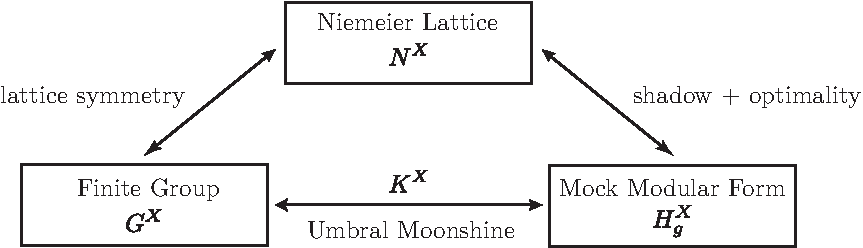
\includegraphics[width=0.92\linewidth]{figures/fig3_umbral_construction.pdf}
    \caption{本影月光的构造。（原文 p.52，图 2）图中：由 Niemeier 格 $N^X$ 的格对称性得到有限群 $G^X$；由影（shadow）与最优性得到模拟模函数 $H^X_g$；下方双箭头即本影月光。}
    \label{UM_construction}
  \end{center}
\end{figure}

指定好 $\SL_2(\ZZ)$ 的模拟 Jacobi 形式之后，为描述月光关系，我们还需要一族模拟 Jacobi 形式
$\psi^X_g= \sum_r H_{g,r}^X\theta_{m,r}$：$\SL_2(\ZZ)$ 的每个子群对应一族，$G^X$ 的每个共轭类 $[g]\subset G^X$ 对应其中一员。
模拟模形式 $H^X_g=(H^X_{g,r})$ 于是扮演本影月光模的分次特征标，如猜想 \ref{conj:mock_umbral} 所述。
这可以在很大程度上仿照 $\SL_2(\ZZ)$ 情形实现，不过会出现额外的微妙之处，需要格外小心。
更多细节参见 \cite{cheng2018weight}。

一旦指定了模拟模形式 $H^X_g$，逐项验证猜想 \ref{conj:mock_umbral} 中 $G^X$-模 $K_{r,D}^X$ 的存在性就是平凡的，即每次只验证一个 $D$。
此外，整个本影模 $K^X=\bigoplus_r \bigoplus_D K_{r,D}^X$ 的存在性，已利用（模拟）模形式的性质得到数学证明 \cite{gannon2016much,DuncanGriffinOno}。
然而，$K^X$ 的构造、甚至对其确切本性的理解，在一般情况下仍然缺失。
迄今只在若干特别简单的本影月光情形中构造出了 $K^X$，对应的 Niemeier 根系为
$3 E_8$ \cite{duncan2017umbral}，$4A_6$ 与 $2A_{12}$ \cite{Duncan:2017bhh}，$4D_6$、$3D_8$、$2D_{12}$ 与 $D_{24}$ \cite{Cheng:2017grj}，以及 $6D_4$ \cite{Anagiannis:2017src}。
\cite{duncan2017umbral} 的构造依赖于模拟模形式 $H^{3E_8}_{g,r}$ 所满足的特殊恒等式，这些恒等式把它与一类格和联系起来；
而 \cite{Duncan:2017bhh,Cheng:2017grj} 则把与 $\Psi^X_{g}$ 相关的亚纯 Jacobi 形式解释为某些顶点算子代数（或手征共形场论）的 twined 配分函数，并用它构造相应的模。
\cite{Anagiannis:2017src} 利用（twined）$K3$ 椭圆亏格、本影月光与 Conway 月光之间的关系，构造了本影月光 $6D_4$ 情形的模；这一关系将在第 \ref{sec:umK3} 节解释。
注意，这是迄今唯一一个构造出来的模，其对应的本影群（嵌入 $\Co_0$ 时）不固定 $\Co_0$ 的 24 维表示中的某个 4-平面。
其意义将在第 \ref{sec:symK3} 节讨论。

% [Tutor Note: 所谓“逐项验证是平凡的”指：每个固定 $D$ 上，$H^X_{g,r}$ 的系数是已算好的非负整数，对照 $G^X$ 的特征标表即可判定该分次分量作为 $G^X$-模存在。真正的困难在于把无穷多个 $D$ 的分量统一成一个自然模 $K^X$——整体存在性要靠 (mock) 模形式的性质（Gannon 与 Duncan–Griffin–Ono 的定理），而统一构造至今没有。]

此外，与第 \ref{sec:mm} 节讨论的广义魔群月光类似的广义本影月光，已在 \cite{GUM} 中建立；
这暗示本影月光模 $K^X$ 上应当存在某些共形场论/模张量范畴结构的要素。
尽管有这些结果，公允地说，给出与本影月光的统一描述相称的本影模的统一构造，仍是当前月光研究最大的挑战之一。

在结束本影月光的综述之前，我们指出本影月光的一个特殊性质，称为\emph{判别式性质}（discriminant property）。
它把判别式 $D$（即 $q$ 级数 $H^X_r$ 中各项 $q^{-D/4m}$ 的幂次）与 $K_{r,D}^X$ 中出现的表示的特征标所生成的数域联系起来。
例如在 $X=24A_1$ 的情形，$H_g= H^{24A_1}_{g,1}$ 中 $q^{7/8}$ 项背后的 $M_{24}$-表示为 $K^{24A_1}_{-7} = \rho \oplus \rho^\ast$，
其中 $\rho$ 是 45 维不可约表示，$\rho^\ast$ 是其对偶表示。
同时，$\tr_\rho g$（从而 $\tr_{\rho^\ast} g$）生成域 $\QQ(\sqrt{-7})$。
只要 $\QQ(D)=\QQ(-7)$，类似关系就随 $q$ 幂次的增大延续下去；而且类似性质对全部 23 个本影月光实例一致成立。
目前人们对此惊人而看似深刻的性质尚无物理上的理解。

% [Tutor Note: 判别式性质说：$q^{-D/4m}$ 项的 $G^X$-表示，其特征标取值落在 $\QQ(\sqrt{D})$ 中；$X=24A_1$、$D=-7$ 时就是 $\QQ(\sqrt{-7})$。这与 Ogg 关于“素数 $p$ 整除魔群阶当且仅当 $X_0(p)$ 亏格为零”的著名观察同一风味：表示论数据“知道”二次域。原文强调目前没有物理解释，勿把它当成已知机制。]

\subsection{Thompson 月光}

Thompson 散在群 $\Th$ 是魔群的一个子群，阶为 $|{\rm \it \Th}|\sim9\cdot10^{16}$，含有 $48$ 个共轭类。
Thompson 月光描述 $\Th$ 的表示论与某些权重 $1/2$ 的弱全纯模形式之间的特殊关系。
它最早在 \cite{Harvey:2015mca} 中讨论，是所谓\emph{斜全纯月光}（skew-holomorphic moonshine）\cite{skew_hol_moonshine} 的第一个实例；
后者把斜全纯 Jacobi 形式与有限群表示联系起来。
关于斜全纯 Jacobi 形式的更多数学与物理信息，参见第 \ref{subsec:shjacobiforms} 节与第 \ref{sec:other_physics} 节。

与 Mathieu 月光和本影月光一样，Thompson 月光把与魔群相联系的有限群（参见第 \ref{sec:sporadic_lattices} 节）与权重 $1/2$ 的模对象联系起来。
不过，它有几处不同。
第一，Thompson 月光中的模对象是模形式，而本影月光中的是影子非零的模拟模形式。
第二，Thompson 月光模带有超结构，即表示带有符号。参见猜想 \ref{conj:thompson}。
话虽如此，这一额外的 $\ZZ_2$-分次结构非常简单，完全由 $m \xmod 4$ 控制，其中 $m$ 是对应于月光函数中 $q$ 的幂次的自然 $\ZZ$-分次。
最后我们指出，Thompson 月光也具有与第 \ref{sec:umbral} 节末尾所讨论的本影月光类似的判别式性质。

% [Tutor Note: 超迹 $\str_{W_m}$ 并非普通迹：在超空间 $\ZZ_2$-分次下它取偶部减奇部。该分次由 $m \bmod 4$ 决定——$m\geq0$ 且 $m\equiv0\bmod4$ 或 $m=-3$ 时为偶，其余为奇；允许的 $m$ 只需 $m\equiv0,1\bmod4$，故奇部（带负号）只出现在 $m\equiv1\bmod4$ 的项上，这正是下面 (5.24) 中 $q^5$ 项系数带负号的原因。]

为了描述 Thompson 月光，我们从如下猜想开始 \cite{Harvey:2015mca}：
{\conj \label{conj:thompson} 存在一个 $\ZZ$-分次 $\Th$-超模（参见 \eq{def:supermodule}）
\begin{equation}
W=\bigoplus_{m\geq-3\atop m\equiv0,1\bmod4}^\infty W_m~
\end{equation}
使得 $W_m$ 的分次维数与某个权重 $1/2$ 的弱全纯模形式 $\mathcal{F}_3$ (\ref{eq:F3}) 之间有关系
\begin{equation}
\mathcal{F}_3(\tau)=\sum_{m=-3\atop m\equiv0,1\bmod4}{\str}_{W_m}(1)q^m~.
\end{equation}
此外，相应的 McKay-Thompson 级数
\begin{equation}
\mathcal{F}_{3,g}(\tau)=\sum_{m=-3\atop m\equiv0,1\bmod4}{\str}_{W_m}(g)q^m~,
\end{equation}
由某些权重 $1/2$ 的弱全纯模形式给出，
且 $\mathcal{F}_{3,e}=\mathcal{F}_3$。
最后，若 $m\geq0$ 且 $m\equiv0\bmod4$，或 $m=-3$，则 $W_m$ 在超空间 $\ZZ_2$-分次下为偶；否则为奇。
}\\

\noindent 下面讨论这一猜想的各个要素。函数 $\mathcal{F}_3$ 定义为
\begin{equation}
\label{eq:F3}
\mathcal{F}_3(\tau):=2f_3(\tau)+248\theta(\tau)~,
\end{equation}
其中 $\theta(\tau)$ 是第 \ref{subsec:modular_forms} 节讨论的 Jacobi theta 函数。
下面说明 $f_3$ 的取法。

把 Kohnen-plus 空间 $M_{1/2}^+$ 定义为这样的全纯函数之集：它们像 $\theta$ 一样变换，
并且在 Fourier 展开 $\sum c(n)q^n$ 中额外满足 $c(n)=0~\forall~n\neq0,1\bmod4$。
可以证明，$M_{1/2}^+$ 其实是一维的，由 $\theta$ 本身张成。
然而，若允许尖点处有极点，就得到 Kohnen-plus 空间中权重 $1/2$ 的弱全纯模形式构成的非平凡空间 $M_{1/2}^{!,+}$。
\cite{Zag_TrcSngMdl} 中，Zagier 为 $M_{1/2}^{!,+}$ 构造了一组无穷维基，由如下（唯一的）函数张成：
\begin{equation}
f_d(\tau)=q^{-d}+\sum_{n>0}A(n,d)q^n~,~~d\equiv0,3\bmod4~,
\end{equation}
其中 $f_0=\theta$。这里我们主要关心 $d=3$ 的情形。

% [Tutor Note: Kohnen-plus 空间的“plus”条件 $c(n)=0$（$n\not\equiv0,1\bmod4$）等价于权 $1/2$ 情形的一个 Fricke 本征条件；正是一维性（$M^+_{1/2}=\CC\,\theta$）与允许尖点极点后得到的 $M^{!,+}_{1/2}$ 里出现 $q^{-3}$ 极项，才使 Thompson 月光能把极项 $2q^{-3}$ 作为 Rademacher 和的唯一输入。]

利用唯一性容易证明，$f_3$ 可显式写成
\begin{equation}
\label{eq:by_hand_f3}
f_3(\tau)=-\frac{1}{20}\left(\frac{[\theta(\tau),E_{10}(4\tau)]}{\Delta(4\tau)}+608\theta(\tau)\right)=q^{-3}-248q+26752q^4-\dots~,
\end{equation}
其中 $E_{10}=E_4E_6$ 是权重 10 的 Eisenstein 级数，$\Delta$ 是第 \ref{subsec:modular_forms} 节引入的权重 12 尖形式。
\emph{Rankin-Cohen 括号}定义为 $[f,g]:=kfDg-lgDf$，其中 $D=\frac{1}{2\pi i}\frac{d}{d\tau}$，$k,l$ 分别是模形式 $f,g$ 的权重。

Thompson 月光始于如下观察：$f_3$ 的前几个 Fourier 系数可以用 $\Th$ 的不可约表示维数表示。
例如 $1=1$、$248=248$、$26752=27000-248$。
值得注意的是，$f_3$ 与 $\Th$ 之间的这一联系早已出现在广义魔群月光的语境中 \cite{DixonL.1988Batb,BorcherdsRichard1995AfoO,MR2904095}，参见第 \ref{sec:mm} 节。
具体地说，$\MM$ 的类 $3C$ 的中心化子同构于 $\mathbb{Z}_3\times\Th$ \cite{conway_norton}，因此扭模 $V^\natural_{3\text{C}}$ 带有 $\Th$ 的自然作用。
相应的扭广义特征标由 $f_3$ 的所谓 \emph{Borcherd's lift} 给出：
\begin{equation}
Z(3\text{C},e;\tau)=q^{-\frac{1}{3}}\prod_{n>0}(1-q^n)^{A(n^2,3)}~.
\end{equation}
但请注意，上述与广义魔群月光的联系只限于 $f_3$ 的系数 $A(n^2,3)$，并不能解释为何其余系数也与 $\Th$ 有关系。

% [Tutor Note: $248$ 是 $\Th$ 最小的非平凡不可约表示维数（也等于 $E_8$ 伴随表示的维数），$27000$ 也是 $\Th$ 的不可约表示维数；$26752=27000-248$ 中的负号不是笔误，而是超迹中奇部的符号，与猜想 \ref{conj:thompson} 的 $\ZZ_2$-分次一致。作者特意选这个例子，是因为三项都直接对应 $\Th$ 的表示维数。]

% 原文 p.54 把 Borcherds 的姓氏拼作 “Borcherd's lift”，译文照录原名，未作改动。

为了做得更好，\cite{Harvey:2015mca} 的想法是“修正”该函数，把 theta 函数 $\theta(\t)$ 的额外贡献纳入进来，转而考虑
\begin{equation}
\mathcal{F}_3(\tau):=2f_3(\tau)+248\theta(\tau)=2q^{-3}+248+2\cdot27000q^4-2\cdot85995q^5+\dots~, 
\end{equation}
它属于 Kohnen-plus 空间。
注意交替的符号对应于猜想 \ref{conj:thompson} 中提到的超空间结构。

Thompson 月光的 McKay--Thompson 级数 ${\cal F}_{3,g}$ 具有与上述非常相似的结构。
概略地说，它们最自然地可看作两项之和
\be\label{thompson_mckaythompson}
{\cal F}_{3,g} = {\text{投影 Rademacher 和}} + \th{\text{ 修正}}~,
\ee
其中第一项是唯一的极项 $2q^{-3}$ 对适当群 $\Gamma_g$ 与乘子系统所作的 Rademacher 和，再投影到 Kohnen-plus 空间；
第二项同样涉及 $\theta(d^2\t)$ 的线性组合，其中 $d$ 是与群 $\Gamma_g$ 相容的某些整数。
更多细节参见 \cite{Harvey:2015mca}，尤其是 \cite{GriffinMichael2016Apot}。

值得注意的是，Thompson 月光中的模对象与所谓的奇异模迹（traces of singular moduli）有密切关系，后者是数论中的重要量。
如第 \ref{subsec:MMF} 节最后一个例子所述，奇异模迹的生成函数具有有趣的模性质 \cite{Zag_TrcSngMdl}。
特别地，有
\begin{equation}
A(n,3)=\frac{1}{\sqrt{n}}\sum_{Q\in\mathcal{Q}_{-3n}/\PSL_2(\ZZ)}\chi_{n,-3}(Q)J(\alpha_Q)~,~~n\in\ZZ_+~,
\end{equation}
它与参与 Thompson 月光的模形式 $f_3$ 的 Fourier 系数一致。
上式中 $\chi_{n,-3}$ 表示某个亏格特征标，其精确定义可在 \cite{Zag_TrcSngMdl} 中找到。
若只跟踪二次型的 $\Gamma_0(N)$-等价类，则同样的奇异模迹关系也可在更高水平上建立。

% [Tutor Note: 这里的 $J$ 是奇异模迹定义中归一化的 $j$-函数（$J=j-744=q^{-1}+O(q)$），$\alpha_Q$ 是二次型 $Q$ 对应的虚二次点；求和跑遍判别式 $-3n$ 的二次型在 $\PSL_2(\ZZ)$ 下的类，$\chi_{n,-3}$ 是相应的亏格特征标。Zagier 定理把这组迹的生成函数识别为 $f_3$，于是数论的类数信息与 Thompson 月光的系数是同一批整数。]


% ==================== 内联自 chapters/ch06_moonshine32.tex ====================
% ===================================================================
%  第 6 节 权重 3/2 处的月光（Moonshine at weight three-halves）
%  原文：TASI10.tex 第 2073--2124 行（PDF p.55--57）
% ===================================================================
\section{权重 $3/2$ 处的月光}
\label{ch:moonshineweight32}

\begin{keytakeaways}
  \item 权重 $3/2$ 的月光目前只有两个确立的例子：\emph{O'Nan 月光}把一组权 $3/2$ 模拟模形式与 O'Nan 群相联系；\emph{类数月光}（class number moonshine）则由 Hurwitz–Kronecker 类数构造出容纳无穷多个群 $\ZZ_p$ 的一族模拟模形式。
  \item 与权 $0$、权 $1/2$ 的月光不同，权 $3/2$ 的模拟模形式不由模性与解析性唯一确定，其 Fourier 系数显著地受权 $3/2$ 尖形式支配。
  \item 超模在这里是内在而不可避免的：同一 $q$ 幂的 Fourier 系数可以是群表示迹的差，因而必须使用超迹。
  \item 权 $3/2$ 尖形式通过 Shimura 对应与 Waldspurger 型关系连接椭圆曲线的特殊 $L$ 值，把月光与算术几何、Tate–Shafarevich 群联系起来。
  \item 月光型联系可能普遍存在：除 pariah 散在群之外，有限单群分类中非散在单群的一个无限族 $\ZZ_p$ 也参与其中；这给物理提出了构造相应超模的挑战。
\end{keytakeaways}

这是一个当前发展迅速的月光研究领域。因此我们将写得非常简略，只突出近期发展的若干关键特征与前景。

% [Tutor Note: 权重 $k$ 的模形式在 Serre 对偶下的配对权重是 $2-k$，所以 $w=1/2$ 的对偶权重为 $2-1/2=3/2$。原文写成 $w=2-\frac{1}{2}=\frac{3}{2}$ 正是强调这一点；不要误记为 $w=1/2+1$，也不要把 $2-w$ 与 $1-w$ 混用。]

在对权重 $1/2$ 的月光作了富有成果的探索之后，人们自然会追问对偶权重——
$w=2-\frac{1}{2}=\frac{3}{2}$——的月光图景。
权重 $3\over 2$ 的模拟模形式所受的约束远少于权重 $1\over 2$ 的对应物，
结果它们为研究有限群联系提供了肥沃的土壤，已经带给我们
\emph{O'Nan 月光} \cite{onan} 与 \emph{类数月光} \cite{class_nr_moonshine}；
后者涉及 \eq{hurwitz_mock} 中描述的 Hurwitz–Kronecker 类数模拟模形式。

% [Tutor Note: Hurwitz–Kronecker 类数 $H(N)$ 是判别式 $-N$ 的整二次型在 $\PSL_2(\ZZ)$ 下的类数（按自同构群大小加权），其生成函数 ${\cal H}(\tau)=\sum_{N\ge 0}H(N)q^N$ 是权 $3/2$、水平 $4$ 的模拟模形式，影子正比于 theta 函数 $\sum_{n\in\ZZ}q^{n^2}$。它就是 \eq{hurwitz_mock} 中的类数模拟模形式；注意它不等于普通类数 $h(-N)$，两者相差一个权因子。]

权重 $3/2$ 中多半还有更多宝藏。这里我们只评论两个已经确立的月光例子。
我们将指出权重 $3/2$ 的这两个月光例子所具有的三个显著性质\footnote{事实上，这些性质使权重 $3/2$ 的联系与迄今讨论的权重零与权重 $1/2$ 的月光例子如此不同，以至于人们会怀疑是否还应当对它们使用“月光”一词。}。

% [Tutor Note: 作者说“多半还有更多宝藏”而未给论证。实质原因是权 $1/2$ 的模拟模形式受 Serre–Stark 型定理的强约束（全纯部分几乎由 theta 函数决定），而权 $3/2$ 没有相应定理，可承载的群表示自由度大得多；因此“更多例子存在”是一个经验判断，不是定理。]

\myparagraph{超模}

在 \S\ref{cha:weight0} 讨论的魔群月光与 Conway 月光中，底层的模是“实”模（相对于超模 \eq{def:supermodule}），
所涉及的群特征标是普通迹（相对于超迹）。
Mathieu 月光与本影月光中也是如此，只是 \eq{rep_mock_umbral} 中的极点项例外：
它们的系数为负，却不携带任何关于群表示的非平凡信息。
在 Thompson 月光中我们遇到超模，但方式相当平凡：超模是纯偶的还是纯奇的，
取决于相应的 $q$ 幂在模 $4$ 下是 $+1$ 还是 $-1$。
特别地，在权重 $1/2$ 中我们不会遇到这样的月光例子：模拟模形式的 Fourier 系数
由群表示迹的差给出，也就是说，在每个齐次分量中超模总是要么为偶、要么为奇。

% [Tutor Note: 超模 \eq{def:supermodule} 指 $\ZZ_2$ 分次模，偶分量的维数减奇分量的维数给出超迹 Str。在权 $1/2$ 的 Thompson 月光中，按 $q$ 幂模 $4$ 的取值 $+1$ 或 $-1$，每个齐次分量整体取偶或整体取奇，所以普通迹已经够用；权 $3/2$ 中同一齐次分量可以同时含偶、奇部分，普通迹会丢掉信息，必须使用超迹。]

在权重 $3/2$ 中这不再成立：超模的“超”性质是我们讨论的这两个月光例子内在且不可避免的特征。

\myparagraph{尖形式}

在迄今讨论的月光例子中，所涉及的（模拟）模对象都十分特殊：它们本质上由自身的模性质与解析性质唯一确定。
特别地，魔群月光与 Conway 月光的分次特征标（graded characters）是 Hauptmodul，
在一个可加常数之内可以写成只含单个极点项 $q^{-1}$ 的 Rademacher 和。
本影月光（包括 Mathieu 月光）与 Thompson 月光的分次特征标，在加上 theta 函数之后也是（投影）Rademacher 和
（参见 \eq{thompson_mckaythompson} 与 \cite{cheng2018weight}）。
后者可以说只是一个小修正：除极少数指数外，theta 函数的系数都为零
（除非指数在某个特定的重标度下为平方数），而且它们不携带任何有趣的数论信息。

% [Tutor Note: “由模性与解析性本质唯一确定”一语省略了论证：给定权、给定同余子群与给定极点结构（此处是单个 $q^{-1}$），Rademacher 和给出唯一的模对象；极点结构本身又由可复制性（replicability）约束固定。这正是权 $0$ 与权 $1/2$ 月光能用少量数据确定整条 $q$ 级数的原因。]

% [Tutor Note: theta 函数的系数只在（重标度后的）平方数处非零，所以“加上 theta 函数”只修正极少数 $q$ 幂。但 theta 函数系数本身不含群表示信息，不要把它当成月光内容的一部分，也不要据此认为整个模对象仍未确定。]

这个关键的唯一性性质曾用来区分权重零与权重 $1/2$ 月光的模拟模形式；
在权重 $3/2$ 的月光中，它不再是相关的判据。
O'Nan 月光与 类数月光中的模拟模形式，以非常显著的方式涉及权重 $3/2$ 的尖形式。
（尖形式的定义见 \S\ref{subsec:modular_forms} 末尾。）

这一性质打开了与算术几何——数学中一个完全不同的领域——相联系的大门。
这一联系的主要要素是：1）在所谓的 Shimura 对应 \cite{MR783554} 之下，
权重 $3/2$ 新形式的系数与相应权重二新形式的特殊 $L$ 值之间的 Waldspurger 型关系。
2）把椭圆曲线的 $L$ 函数与某些权重二新形式的 $L$ 函数联系起来的模性定理。
3）Birch–Swinnerton-Dyer 猜想（的强形式）（及其已证明的部分）：
它把椭圆曲线的特殊 $L$ 值与它们的重要算术数据——包括 Tate–Shafarevich 群的阶——联系起来。
参见 \cite{MR833192,MR954295,MR3148103}。
4）月光模对象之间的同余，源自特征标之间的同余，后者是有限群表示的基本性质。

% [Tutor Note: Waldspurger 公式给出的是系数平方与特殊 $L$ 值的比例关系（通常形如 $|a_f(|D|)|^2$ 正比于 $L(f,1)$，差 $|D|$ 的幂次与局部因子），并非系数本身与 $L$ 值成线性正比；此外权 $3/2$ 新形式与权 $2$ 新形式之间的对应是 Shimura 对应，不是恒等映射，引用 \cite{MR783554} 时勿把方向弄反。]

% [Tutor Note: 作者把 BSD 列为第三项，是因为 BSD 把 $L(E,1)$ 的零点阶与调节子、挠子群、以及 Tate–Shafarevich 群的阶联系起来；与第 1、2 项合用，才能把权 $3/2$ 系数之间的同余翻译成该群 $p$ 部分的陈述。注意这里同时用到 BSD 的“强形式”与“已证部分”，结论中凡依赖未证部分者都是条件性的。]

综合以上要素，权重 $3/2$ 尖形式与有限群之间的联系引出一系列无穷多的、
关于 Tate–Shafarevich 群 $p$ 部分的陈述，而这些陈述由有限群结构组织起来。
此外，在 类数月光中，附着于某些模数据的椭圆曲线（以及一般的其他阿贝尔簇）的挠子群，
在构造月光模拟模形式时起重要作用。
探索模拟模形式中的有限群结构在算术几何中的含义，是月光研究中一个有趣的新数学方向。

\myparagraph{新的有限群}

上述两个性质分别涉及月光联系的有限群一侧与模形式一侧，
它们使权重 $3/2$ 月光有可能把新类型的有限群纳入月光的领域。

O'Nan 月光，顾名思义，把一组权重 $3/2$ 的模拟模形式与 O'Nan 群联系起来。
O'Nan 群于 1976 年在有限群分类的紧张发展中被发现，是与魔群无关的 6 个 pariah 群之一。
另一方面，类数月光给出由 Hurwitz–Kronecker 类数 \eq{def:hurwitz} 产生的
无穷多个权重 $3/2$ 模拟模形式构成的一族，它容纳\emph{无穷多个群}的表示。
回忆一下：在有限单群的分类中，除散在群之外还有三个无限族，
其中之一是素数阶 $p$ 的循环群 $\ZZ_p$。

% [Tutor Note: 原文 “cycle groups” 应为 “cyclic groups”（循环群）之误：有限单群分类中的三个无限族是 $\ZZ_p$（$p$ 为素数）、交错群 $A_n$（$n\ge 5$）与 Lie 型（Chevalley）群；本句随后只用到 $\ZZ_p$。译文按“循环群”处理，原词登记为疑似笔误，页面图像 PDF p.56 亦作 cycle groups。]

% [Tutor Note: 6 个 pariah 群指不参与魔群的散在单群：$J_1$、$J_3$、$J_4$、$\mathrm{Ly}$、$\mathrm{O'N}$、$\mathrm{Ru}$。O'Nan 群由 O'Nan 于 1976 年构造，阶为 $2^9\cdot 3^4\cdot 5\cdot 7^3\cdot 11\cdot 19\cdot 31$。它出现在魔群月光之外，正是本节强调“月光不限于魔群”的关键例证。]

结果表明，对每个素数 $p$，都有一个水平 $4$ 的模拟模形式 ${\cal H}_{p,1}$——
它是 类数模拟模形式 ${\cal H}$ \eq{hurwitz_mock} 的标量倍——
以及一个水平 $4p$ 的模拟模形式 ${\cal H}_{p,p}$，
使得它们与 $\ZZ_p$ 的一个 $\ZZ$ 分次超模的两个分次特征标相符。

% [Tutor Note: 对 $\ZZ_p$ 而言不可约表示都是一维的（特征标取 $p$ 次单位根），所以两个分次特征标足以编码整个超模；水平 $4$ 与 $4p$ 正对应未扭与 $\ZZ_p$ 扭结扇区（twisted sector）的模参数，因此 $\ZZ_p$ 的“无穷族”恰好对应一族按 $p$ 增长的模形式。]

除了这个无限的群族之外，\cite{class_nr_moonshine} 还表明，
不同水平（由群元阶的 4 倍给出）的模拟模形式共同编码了有趣的 Mathieu 群的超模。

这些权重 $3/2$ 月光的实例大大拓宽了模对象与有限群之间联系的视野。
权重零与权重 $1/2$ 的所有月光实例都与和魔群有关的群相联系，
但 O'Nan 例子与类数例子表明，情况未必如此。
在这些例子中已经证明：一个 pariah 散在群，以及三个非散在有限单群无限族之一，
也以类似方式与（模拟）模形式相联系！
这暗示了一种诱人的可能性：月光型联系其实是普遍的，是模对象与有限群图景中的内在性质；
而有限群是模对象的一种重要组织性结构。

最后但同样重要的是，这些涉及无穷多个群的超模的新联系给物理提出了有趣的挑战。
物理还能提供这些有限群模并解释这些联系吗？
如果能够，哪些相关物理系统可以产生这些超模？


\part{月光与弦论}
弦论从最早的时候就对月光起着关键作用：从魔群月光模的共形场论构造，
到 Borcherds 受弦论启发给出的魔群月光证明（参见第 \ref{sec:mm} 节）。
人们也预期弦论会在理解 Mathieu 月光与本影月光中扮演有趣的角色，
并且希望月光能教给我们关于弦紧化某些侧面的新颖而重要的知识。
更一般地说，与物理的联系是许多弦论学家和数学家觉得月光令人兴奋的关键原因之一。
本部分我们将讨论其中一些联系。第 \ref{sec:physics_monstrous} 节概述魔群月光与
某些 $(1+0)$ 维弦紧化之间的关系；第 \ref{chap:moonshineK3} 节——本部分的主要一节——
总结各种月光与 $K3$ 紧化之间的已知关系；最后在第 \ref{sec:other_physics} 节
简要提及近期讨论的其他一些联系。


% ==================== 内联自 chapters/ch07_phys_monstrous.tex ====================
% ===================================================================
%  第 7 节 魔群月光（Monstrous moonshine）
%  原文：TASI10.tex 第 2136--2179 行（PDF p.58--59）
% ===================================================================
\section{魔群月光}
\label{sec:physics_monstrous}

\begin{keytakeaways}
  \item 物理构造的起点是杂化弦紧化到 $1+1$ 维：内部 CFT 的中心荷为 $(24,12)$，由魔群月光模 $V^\natural$ 与 Conway 模 $V_{}^{s\natural}$ 的乘积给出；再紧化空间方向到圆，便得到 $0+1$ 维理论。
  \item 对每个 $g\in\MM$ 作 CHL 型轨道流形化，其第一量子化 BPS 态构成广义 Kac–Moody 代数 $\mathfrak{m_g}$ 的模：$g=e$ 时是 Borcherds 的魔代数，$g\neq e$ 时是 Carnahan 的 twisted 魔代数。
  \item BPS 指标 $Z_{(g,h)}(T,U)$ 可以写成 McKay–Thompson 级数的乘积（\eq{BPSindexmonster}），从而把时空 BPS 态计数与月光函数联系起来。
  \item BPS 指标在自对偶群下的不变性直接给出 $T_g$ 的 $\Gamma_g$ 不变模性；对半径插值的分析又给出 Hauptmodul 性质。
  \item 这条思路为魔群月光的模性与亏格零性质提供了物理解释，是“用弦论实现月光”的范式。
\end{keytakeaways}

本节我们简要描述近期的一个弦论构造，它由 \cite{paquette2016monstrous,Paquette:2017xui} 发展而来，
涉及魔群月光模 $V^\natural$ 以及 \S\ref{sec:mm} 讨论的相伴的扭模（twisted module）$V^\natural_g$。
尽管魔群月光令人瞩目的亏格零性质已在数学上得到证明，其物理解释长期难以捉摸。
近期工作 \cite{paquette2016monstrous,Paquette:2017xui} 通过考虑某些杂化弦理论紧化到 $0+1$ 维的情形，
为这一重要性质提供了线索。

% [Tutor Note: 这里的 $V^\natural_g$ 不是某个独立构造的代数，而是 $V^\natural$ 在 $g$ 作用下的扭模：其分次特征标正是 McKay–Thompson 级数 $T_g$。理解本节的关键是把“群元 $g$ 标注的模块”与“时空 BPS 态空间”对应起来，而不是把 $g$ 当成对称性作用在未扭空间上。]

在 \cite{paquette2016monstrous,Paquette:2017xui} 中，出发点是紧化到 $1+1$ 维，
其内部 CFT 的中心荷为 $(24,12)$，由 $V^\natural\times V_{}^{s\natural}$ 给出。
第二个因子是 \S\ref{sec:conway_moonshine} 引入的 Conway 模，它主要扮演旁观者的角色，
其主要功能是为世界面理论提供右行 $\mathcal{N}=1$ 超对称。
该模型在二维时空中具有 ${\cal N}=(0,24)$ 超对称。
我们进一步把剩余的空间方向紧化在圆上。
这一额外紧化对于计算下文描述的“BPS 指标”以及构造更一般的模型至关重要。

% [Tutor Note: 中心荷 $(24,12)$ 应读作左行 $c=24$、右行 $c=12$：$V^\natural$ 贡献左行 $24$，Conway 模 $V_{}^{s\natural}$ 贡献右行 $12$。右行 $\mathcal{N}=1$ 世界面超对称由 Conway 模提供，这正是后文能用 $(-1)^F$ 定义时空 BPS 指标的前提。]

更一般地，对每个 $g\in\MM$，通过按一个对称性对理论作轨道流形化来构造 CHL 型模型：
该对称性在 $V^\natural$ 上按 $g$ 作用，在圆上则按一个移位作用，其阶由 $g$ 在 $V^\natural$ 上作用的某些性质决定
（在最简单的情形中等于 $g$ 的阶）。
为避免涉及引力反常的微妙之处，该理论应在零弦耦合极限下考虑。

% [Tutor Note: CHL 型模型指 Chaudhuri–Hockney–Lykken 型紧化：在圆上同时作平移与对称性投影，使左右行不对称。圆上移位的阶必须与 $g$ 在 $V^\natural$ 上的作用阶匹配，否则扭结扇区的基态能量不为零、模不变性被破坏；这是构造能自洽的关键约束。]

\cite{paquette2016monstrous} 表明，上述模型的（第一量子化）BPS 态构成广义 Kac–Moody 代数 $\mathfrak{m_g}$ 的模：
当 $g= e$ 时它就是 Borcherds 构造的魔代数，当 $g\neq e$ 时则是 Carnahan 构造的“twisted”魔代数
\cite{Carnahan2008,MR2904095,carnahan2012generalized}。
广义魔群月光的讨论另见 \S\ref{sec:mm}。
我们关心这些理论中计数时空 BPS 态的（twined）BPS 指标。
记相关 Hilbert 空间为 $\mathcal{H}^g_{\text{BPS}}$，我们定义
\begin{equation}
Z_{(g,h)}(T,U):=\tr_{\mathcal{H}^g_{\text{BPS}}}\left((-1)^F \, h \, e^{2\pi iTW}e^{2\pi iUM}\right)~,
\end{equation}
其中 $g,h$ 是魔群中相互对易的元素。

% [Tutor Note: 指标 $Z_{(g,h)}$ 的两个下标含义不同：第一个下标 $g$ 选定扭结扇区，即迹在 $\mathcal{H}^g_{\text{BPS}}$ 上取；第二个下标 $h$ 是插入的群元。只有 $g$ 与 $h$ 对易，$h$ 才保持 $g$-扭结扇区，迹才有定义；这就是原文强调 commuting elements 的原因。]

上式中 $T,U\in \HH$ 分别是绕数（winding）与动量（momentum）量子数 $W,M$ 的复化化学势，
其虚部按逆温度与半径缩放为
\be
\im T \sim {\beta R}~,~~ \im U \sim {\beta \over R}~.
\ee

% [Tutor Note: 指数中 $T$ 配绕数 $W$、$U$ 配动量 $M$，不要写反。绕数能量正比于半径 $R$，动量能量正比于 $1/R$，所以 $\im T\sim\beta R$、$\im U\sim\beta/R$；这里 $T,U$ 是复化化学势，实部给出相位，虚部给出 Boltzmann 型压制。]

利用 $\mathcal{H}^g_{\text{BPS}}$ 的 Fock 空间构造（允许任意数目的自由弦），
以及把无穷乘积与无穷和联系起来的 twisted 分母公式——它推广了 Koike–Norton–Zagier 公式 \eq{eq:replicability_J}——可以得到
\begin{equation}\label{BPSindexmonster}
\begin{split}
&Z_{(e,g)}(T,U)=\left(T_{(e,g)}(T)-T_{(e,g)}(U)\right)^{24} \\
&Z_{(g,e)}(T,U)=\left(T_{(e,g)}(T)-T_{(g,e)}(U)\right)^{24}~.
\end{split}
\end{equation}

% [Tutor Note: 原文如此：第二行右侧为 $T_{(g,e)}(U)$，与第一行 $T_{(e,g)}(U)$ 的下标不对称；可能另有约定（扭模的 twining 方向），也可能是笔误。译文照录，读者引用时请核对原文。阅读时注意 $T_{(e,g)}=T_g$ 才是 McKay–Thompson 级数，不要把 $T_{(g,e)}$ 也当成 $T_g$。]

% [Tutor Note: “twisted 分母公式”指 Borcherds 的 twisted denominator identity（广义 Kac–Moody 代数的 Weyl 分母公式）：它把扭结扇区上的无穷乘积展开为无穷和，其指数正是 $\mathfrak{m_g}$ 的根重数。Koike–Norton–Zagier 公式 \eq{eq:replicability_J} 是 $g=e$ 时的特例；作者略去了该恒等式的证明。]

注意 $T_{(e,g)}=T_g$ 是魔群月光的 McKay–Thompson 级数。

上述表达式给出魔群月光的模性与亏格零性质的物理解释。

% [Tutor Note: $Z_{(g,e)}$ 取 $1/24$ 次幂后与 $T_g$ 同阶：$Z_{(g,e)}(T,U)^{1/24}$ 在 $T\to i\infty$ 时的发散对应 $T_g$ 的极点项 $q^{-1}$。这个 $1/24$ 次幂来自 24 个横方向自由弦因子的乘积，指数极易漏掉；不要把 $1/24$ 误写成 $1/2$ 或 $24$。]

首先，\cite{paquette2016monstrous} 利用 \cite{Persson:2015jka} 发展的技巧表明，
自对偶群（即 T 对偶群的一个子群，它在同一个 CHL 模型之间作映射，但一般在不同的模值处）
涉及 $\SL_2(\RR)$ 的两个子群，它们在 \eq{BPSindexmonster} 中分别独立地作用于 $T$ 与 $U$。
特别地，作用于 $T$ 的 $\SL_2(\RR)$ 子群正是 $\Gamma_g$，即魔群月光中相应的亏格零群
（参见猜想 \ref{conj:conwa_norton}）。
因此，BPS 指标在自对偶群下的物理不变性立即给出月光函数 $T_{g}(T)$ 的 $\Gamma_g$ 不变模性。

% [Tutor Note: 自对偶群是 T 对偶群中保持同一个 CHL 模型（可以取不同模值）的子群；它能分解为分别作用在 $T$ 与 $U$ 上的两个 $\SL_2(\RR)$ 子群，这是二维环面紧化的结构使然。作用在 $T$ 上的那个子群恰为亏格零群 $\Gamma_g$，所以指标的模不变性“翻译”成 $T_g$ 的模性；注意这里不需要证明 $T_g$ 模性，它是物理不变性的推论。]

其次，回忆 $T_{(e,g)}$ 的 Hauptmodul 性质可以重新表述为：
它们只在 $\tau\rightarrow i\infty$ 及其在 $\Gamma_g$ 下的像处有单个极点。
用超对称指标的语言，这意味着对固定的 $U$，$Z_{(g,e)}(T,U)^{1/24}$ 及其 T 对偶像在 $T\rightarrow i\infty$ 时发散。
利用 T 对偶
\[
Z_{(e,g)}(T,U)=-Z_{(e,g)}\left(-\frac{1}{U},-\frac{1}{T}\right)
\]
以及 $T_{(g^ah^c,g^bh^d)}(\tau)$ 与 $T_{(g,h)}\left(\frac{a\tau+b}{c\tau+d}\right)$ 之间的广义月光关系
（参见 \S\ref{sec:mm}），这一性质就转化为如下陈述：
对所有互素整数 $a$ 与 $b$，当 $T$ 固定时 $Z_{(g^a,g^b)}(T,U)$ 在 $U\to i\infty$ 的极限下发散，
当且仅当该极限通过某个与 $g\in \MM$ 相联系的 CHL 模型的自对偶，
与 $T\to i\infty$（$U$ 固定）的极限相联系。

% [Tutor Note: 上式 T 对偶的整体负号极易漏掉：$Z_{(e,g)}(T,U)=-Z_{(e,g)}(-1/U,-1/T)$ 同时交换了 $T$ 与 $U$、各自取倒数，并带一个负号。注意 $(f(T)-f(U))^{24}$ 在 $T\leftrightarrow U$ 下因指数为偶数并不变号，所以这个负号是原文式子的独立成分，照录即可，不要自行“修正”为加号；若改成加号，后文用 T 对偶连接两个极限的论证将不成立。]

下面我们从物理考虑论证这一点为何成立。
让我们通过改变半径 $R$ 在两个极限之间插值，同时把逆温度 $\beta$ 固定得很大。
在低温极限下，固定 $U$、$T\to i\infty$ 处的发散由基态贡献 $e^{\beta R}$ 引起，它在 $R\to \infty$ 时爆炸。
小半径极限是收敛的，除非发生相变，使得在临界线的另一侧出现贡献为 $e^{\beta / R}$ 的新基态。
若发生这种情况，可以证明在临界线上的自对偶半径极限处存在 $SU(2)$ 对称性，
它特别包含一个 T 对偶变换。
换言之，临界线两侧由包含在 $\Gamma_g$ 中的一个自对偶相联系，这就证明了 Hauptmodul 性质。

% [Tutor Note: 作者在此跳过论证的一步是：自对偶半径 $R=\sqrt{\alpha'}$ 处，圆上的 $U(1)_L\times U(1)_R$ 会增强为 $SU(2)_L\times SU(2)_R$（本情形只剩一个 $SU(2)$），其 Weyl 群包含 $R\leftrightarrow 1/R$ 的 T 对偶。正是这个增强对称性保证相变两侧的基态由自对偶联系，从而把“单极点”翻译成 Hauptmodul 性质；完整论证见 \cite{paquette2016monstrous}。]

% [Tutor Note: “$0+1$ 维”即 0 个空间维加 1 个时间维（量子力学）；原文第一部分引言处写作 “$(1+0)$-dimensional”，两种写法指同一次紧化，不要误认为先紧化到两个不同维数。紧化链是：10 维杂化弦 → 2 维（内部 $(24,12)$ CFT）→ 圆紧化 → $0+1$ 维。]


% ==================== 内联自 chapters/ch08_phys_k3.tex ====================
% ===================================================================
%  第 8 节 月光与 K3 弦论  原文：TASI10.tex 第 2180--2454 行（PDF p.59--68）
% ===================================================================
\section{月光与 $K3$ 弦论}
\label{chap:moonshineK3}

\begin{keytakeaways}
  \item 核心物理图像：$K3$ 是除四环面外唯一的二维 Calabi--Yau 流形；其 sigma 模型左右两侧的超共形对称性都增强为 ${\cal N}=4$，这正是 Mathieu 月光能在 $K3$ 椭圆亏格中现身的根源。
  \item 数学工具一：把 $K3$ 椭圆亏格按 ${\cal N}=4$ 短/长多重态的特征标展开（式 \eq{massless_characters}--\eq{massive_characters}），有质量多重态的重数 $c_H(n)$ 即 $M_{24}$-模 $K$ 的分次维数。
  \item 数学工具二：改用 ADE 根系标记的奇点椭圆亏格，把同一分解写成 23 个 Niemeier 格对应的等式 \eq{um_splitEG}，从而把 Mathieu 情形推广到全部本影月光。
  \item 重要结论：Witten 指标只收到 $({\rm massless}_L\times{\rm massless}_R)$ 的贡献，故 $K3$ 椭圆亏格由 20 个 ${\cal N}=4$ 短多重态、负系数的短多重态项 $-2\,ch_{1/4,1/2}$ 与有质量项组成；twining 后的 $\phi_g^X$ 只有在 $g$ 保持四平面时才有 $K3$ sigma 模型的几何实现。
  \item 开放问题：只保持两平面的群元素所对应的本影月光函数尚无物理解释；第 \ref{subsec:phys_Other directions} 节列出的非微扰方向（合并对称性、低维紧化、杂化 $K3$、NS5-膜、VOA）目前均无定论。
\end{keytakeaways}

如 \S\ref{sec:Moonshine at weight one-half} 所述，Mathieu 月光最初是在 $K3$ sigma 模型的背景下被注意到的，后来才被认作本影月光 23 个实例之一。下面将会看到，本影月光的全部实例（而不只是 Mathieu 月光）都与同一个量密切相关，即 $K3$ 椭圆亏格。它刻画 $K3$ sigma 模型的 BPS 态，更一般地也刻画含 $K3$ 曲面的超弦紧化的 BPS 态。正是这种与 $K3$ 弦论的可能联系，使 Mathieu 月光与本影月光对许多弦论学家如此有趣。

% [Tutor Note: 此处“$K3$ 椭圆亏格刻画 BPS 态”应理解为：椭圆亏格是保持超对称的指标，只对短多重态（BPS 态）计数，无质量与有质量短多重态的贡献按 ${\cal N}=4$ 特征标分别归类，故它在模空间中不变。]

这是因为 $K3$ 流形有一个特殊性质：它是二维（复维数）唯一的非平凡（即非环面）Calabi--Yau 流形。由于超对称更多，由此得到的弦论紧化比一般 Calabi--Yau 三维流形上的紧化容易处理得多，所含的结构与信息也比环面紧化丰富得多——后者在许多用途上过于简单而无用。因此，$K3$ 紧化在弦论发展史上一直扮演重要角色，是发展革命性新想法的试验场，包括黑洞微观态计数 \cite{StromingerPhys.Lett.B379:99-1041996} 与 AdS/CFT 对应 \cite{MaldacenaAdv.Theor.Math.Phys.2:231-2521998}。此外，它们还出现在联系不同弦论的重要对偶之中。

% [Tutor Note: 黑洞微观态计数指 Strominger--Vafa 1996 年对五维极值黑洞的工作：把 D-膜构型的态计数与 Bekenstein--Hawking 熵比较，是弦论第一次“数出”黑洞熵；$K3\times S^1$ 紧化正是这类构型的基本例子。]

本节将回顾已观测到的月光与 $K3$ sigma 模型之间的关系，并概述为理解这一关系的起源、以及为找到一个能给出人们迫切想要的本影月光模统一构造的物理系统所必须克服的挑战。最后，我们总结针对这些挑战的各种想法及其现状。

\subsection{Mathieu 月光与 $K3$ 椭圆亏格}
\label{sec:M24moonshine}

如 \S\ref{sec:EG} 所述，$K3$ 的 Calabi--Yau 性质连同 Jacobi 形式性质共同决定：它的椭圆亏格由熟悉的弱 Jacobi 形式 \eq{phi01} 给出，即 $2\f_{0,1}$。回忆：除四环面外，$K3$ 是唯一的二维 Calabi--Yau 流形。它有一个特殊性质：不仅 K\"ahler，而且容许超 K\"ahler 结构。因此，第 \ref{sec:EG} 节讨论的 ${\cal N}=2$ 超共形代数的 $U(1)$ 对称性可以扩充为 $SU(2)$，于是 sigma 模型在左、右 mover 两侧都有增强的 ${\cal N}\!=4$ 超共形对称性。这导致 ${\cal N}=4$ 超共形场论的椭圆亏格有一种特定的分解，下面就来解释。

由于底层的共形场论带有 ${\cal N}=4$ 超共形代数的作用，Hilbert 空间分解为该代数（幺正）不可约表示的直和。于是椭圆亏格 (\ref{elliptic_genus}) 可以写成这些表示的特征标之和，每项带某个重数。把 ${\cal N}=2$ 超共形代数的 $U(1)$ 流代数自然地嵌入 ${\cal N}=4$ 超共形代数的 $SU(2)$ 流代数，只须取 $J_0^3 \sim J_0$。因此 ${\cal N}=4$ 的最高权表示仍由两个量子数 $h,\ell$ 标记，分别对应算子 $L_0$、$J_0^3$；这样的不可约表示 $V_{h,\ell}$ 的特征标定义为
$$
{\it ch}_{h,\ell}(\t,z) := \tr_{V_{h,\ell}} \left( (-1)^{J_0}y^{J_0} q^{L_0-c/24}\right) .
$$
% [Tutor Note: 这里 $J_0^3\sim J_0$ 只表示二者成比例，比例常数取决于 $U(1)$ 流在 $SU(2)$ 中的嵌入约定（常见约定是 $J^{{\cal N}=2}=2J_0^3$）。记号 $\sim$ 正是为了回避这个常数：一旦取定归一化，特征标里 $y^{J_0}$ 的荷与 $\ell$ 的对应才确定，草率地把 $J_0^3$ 当成 $J_0$ 会让 $y$ 的幂次差一个因子。]
对中心荷 $c=6$，Ramond 扇区有两个超对称表示（也称“BPS”表示或“无质量”表示），其量子数为
$$
h=\tfrac{1}{4}\;,\; \ell = 0 ,\tfrac{1}{2} \;.
$$
它们的特征标已算出 \cite{Eguchi1987,Eguchi1988,Eguchi1988a}，为
\bea\label{massless_characters}
{\it ch}_{\frac{1}{4},0}(\t,z) &=& \frac{\th_1^2(\t,z)}{\eta^3(\t)} \m(\t,z)\, ,\\\notag
{\it ch}_{\frac{1}{4},\frac{1}{2}}(\t,z) &=& q^{-\frac{1}{8}} \frac{\th_1(\t,z)}{\eta^3(\t)} - 2 \frac{\th_1(\t,z)^2}{\eta^3(\t)} \m(\t,z)\, ,
\eea 
其中 $\m(\t,z)$ 是所谓的 Appell--Lerch 和，定义见 \eq{def:mu}。

% [Tutor Note: $\m$ 是 Appell--Lerch 和，属于模拟 Jacobi 形式：它本身不满足 Jacobi 形式的模变换，而带一个由影子决定的非全纯修正。正因如此，(8.1) 的两个特征标单独看都不是弱 Jacobi 形式；只有按 (8.3) 组合、并让 $\m$ 与 $\theta_1^2/\eta^3$ 的因子相互补齐之后，$K3$ 椭圆亏格才是模不变的。忽略这一点会把“模拟”误当成“全纯”。]

注意，超对称表示的 Witten 指标不为零：
% [Tutor Note: 原文 p.61 此处第二个式子仍写作 $ch_{1/4,0}$，按上下文（$h=1/4$ 的短多重态有 $\ell=0$ 与 $\ell=1/2$ 两个）应为 $ch_{1/4,1/2}(z=0)=-2$。译文照录原文，读者勿从字面读作两个相同之量。]
$$ch_{\frac{1}{4},0}(\t,z=0) =1\,, \quad ch_{\frac{1}{4},0}(\t,z=0) =-2\,.$$ 
非超对称表示（也称“非 BPS”表示或“”）具有
% [Tutor Note: 原文 p.61 此句第三个引号内空缺，按术语表与上下文应为 massive（“有质量”）。此处照录空缺，语义即“非超对称（或称非 BPS、有质量）表示”。]
$$
h =\tfrac{1}{4} + n\, ,\quad \ell =\tfrac{1}{2}\, ,\quad\text{} \quad n = 1,2,\dots,
$$
其特征标为
\be\label{massive_characters}
ch_{\frac{1}{4}+n,\frac{1}{2}}(\t,z) = q^{-\frac{1}{8}+n} \frac{\th_1^2(\t,z)}{\eta^3(\t)} \, .
\ee
% [Tutor Note: 幂次 $q^{-1/8+n}$ 极易抄错：$c=6$ 时 $-c/24=-1/4$，但 (8.1) 中的指数是 $-1/8$（$c/24$ 的 $1/4$ 已由 $\theta_1,\eta$ 的 $q^{1/8}$ 因子吸收），不要直接写成 $-1/4$。每升高一档有质量能级就多一个 $q$，故一般项为 $q^{-1/8+n}$；$n$ 从 $1$ 起，$n=0$ 的边界即短多重态 $h=1/4$，不属有质量谱。]
按定义，它们对 Witten 指标的贡献为零，即 $ch_{\frac{1}{4}+n,\frac{1}{2}}(\t,z=0) = 0$。这就是为什么 Witten 指标只收到 ${\cal N}=4$ 表示中 (massless$_L\times{\rm massless}_R$) 型量子态的贡献，而椭圆亏格既收到 (massless$_L\times{\rm massless}_R$) 的贡献，也收到 (massive$_L\times{\rm massless}_R$) 的贡献。

现在可以给出 $K3$ 椭圆亏格按 (\ref{splitEGM24}) 分解的第一种物理解释，这一解释使与 $M_{24}$ 的联系变得明显。由 (\ref{splitEGM24}) 以及 \eq{massless_characters}--\eq{massive_characters} 可见，${\bf EG}(K3)$ 可表示为
\be
{\bf EG}(K3) =  20\, ch_{\frac{1}{4},0} -2 \, ch_{\frac{1}{4},{1\over 2}}  + \sum_{n=1}^\infty c_H(n)\,ch_{\frac{1}{4}+n,\frac{1}{2}}
\ee
其中
\be 
H(\t) =q^{-1/8}\left(-2 +\sum_{n=1}^\infty c_H(n)q^n\right) =2 q^{-\frac{1}{8}} \left( -1 + 45\, q+ 231\, q^2 + 770\,q^3\dots \right)
\ee
是 \eq{second_def_H} 给出的模拟模形式。特别地，按 Mathieu 月光猜想 \ref{conj_mock}，有质量多重态的重数 $c_H(n)$ 等于 $M_{24}$-模 $K$ 的齐次分量的维数。

% [Tutor Note: 由 \eq{massive_characters} 后的展开可见 $c_H(1)=90$、$c_H(2)=462$、$c_H(3)=1540$，正是 $M_{24}$ 不可约表示的维数组合：$90=45+45$、$462=231+231$、$1540=770+770$。式中的 $45,231,770$ 是 $H$ 括号内的系数，因整体乘以 $2$ 才得到 $c_H(n)$；漏掉这个因子是常见错误。]

如 \S\ref{subsec:Mathieu} 已提到的，于是人们很自然地想把 $\f_g$ \eq{K3_EG_Fou}（它编码 Mathieu 月光的 McKay--Thompson 级数 $H_g$）认作 $K3$ 非线性 sigma 模型在某个保持 ${\cal N}=4$ 超共形代数的对称性下的 twined 椭圆亏格。对某些 $g\in M_{24}$ 这确实可行，但对另一些群元素，这一解释已被证明不成立。我们将在 \S \ref{sec:symK3} 讨论这一点。

\subsection{本影月光与 $K3$ 椭圆亏格}
\label{sec:umK3}

如前所暗示，对椭圆亏格的分解 (\ref{splitEGM24})——一部分直接来自月光的模拟模形式，另一部分来自 Appell--Lerch 和 $\mu$——${\cal N}=4$ 分解并不是唯一可能的解释。第二种解释以 ADE 根系标记的奇点空间的椭圆亏格为语言，在本例中给出相同结果，但关键差别在于：它可以立刻推广到本影月光其余 22 个实例。

% [Tutor Note: “其余 22 个”来自 Niemeier 格的分类：秩 24 的偶自对偶格共 24 个，其中 Leech 格无根，剩下 23 个带根系的 Niemeier 格 $N^X$ 对应 23 个本影实例；$X=24A_1$ 即 Mathieu 情形，故“其余 22 个”是分类的直接结果，不是巧合数字。]

为说明这一点，我们先给 23 个根系 $X$ 各配一个函数 $\eg(X;\tau,z)$。注意 $K3$ 曲面的一种常见定义是：它至多有 du Val 型曲面奇点，即复平面上形如 $\mathbb C^2/G$ 的奇点，其中 $G$ 是 $SU(2)_{\mathbb C}$ 的有限子群。按著名的 McKay 对应，这些奇点有 ADE 分类。以这些 ADE 奇点为靶空间时，弦论的共形场论描述由 \cite{Ooguri:1995wj} 给出。其椭圆亏格的形式已在多篇文章中研究过，包括 \cite{Troost:2010ud,Eguchi:2010cb,Ashok:2011cy,Ashok:2013pya,Murthy:2013mya,Cheng:2014zpa,Harvey:2014nha}。记 $\eg(Y;\tau,z)$ 为对应于根系 $Y$ 的奇点的椭圆亏格的全纯部分（另见 \S\ref{sec:EG} 末的注记）。把定义扩充到根系之并，$\eg(\cup_i Y_i;\tau,z)= \sum_i \eg( Y_i;\tau,z)$，就得到 23 个 Niemeier 根系 $X$ 各自的 $\eg(X;\tau,z)$ 的定义。例如
\be
\eg(A_1;\tau,z) = ch_{\frac{1}{4},0}(\t,z) = \frac{\th_1^2(\t,z)}{\eta^3(\t)} \m(\t,z), 
\ee
而 $\eg(24A_1;\tau,z) = 24\frac{\th_1^2(\t,z)}{\eta^3(\t)} \m(\t,z)$ 正是 \eq{splitEGM24} 中 $\eg(K3)$ 分解的第一项。

% [Tutor Note: 单个 $A_1$ 奇点给出 $ch_{1/4,0}$ 而非 $ch_{1/4,1/2}$：$A_1$ 是 $\CC^2/\ZZ_2$ 型 du Val 奇点，其椭圆亏格只含无质量表示中最简单的一支。系数 $24$ 来自 $24A_1$ 中 24 个分量相加，故与 (8.3) 中 $20\,ch_{1/4,0}-2\,ch_{1/4,1/2}$ 的 $20$ 不是同一类计数，勿混。]

回忆：对 23 个 Niemeier 格 $N^X$（由根系 $X$ 唯一确定），本影月光对每个 $N^X$ 各配一个有限群 $G^X$，并对每个 $g\in G^X$ 配一个权 1 的模拟 Jacobi 形式 $\psi^X_g = \sum_r H^X_{g,r} \tilde\theta_{m,r}$。\cite{Cheng:2014zpa} 证明 $\eg(K3)$ 有 23 种分成两部分的方式：
\be\label{um_splitEG}
{\bf EG}(K3;\tau,z) = \eg(X;\tau,z) + {\theta_1^2(\tau,z) \over 2\eta^6(\tau)} \left({1\over 2\pi i}{\partial\over \partial w} \psi^X(\tau,w)\right) \Big\lvert_{w=0}
\ee 
其中 $\psi^X =\psi^X_e$ 是 \S\ref{sec:umbral} 给出的最优模拟 Jacobi 形式，编码本影月光模的分次维数；第一项就是上面讨论的奇点椭圆亏格。
% [Tutor Note: 第二项先对 $w$ 求导再取 $w=0$，且 $\theta_1^2$ 前的系数是 $1/(2\eta^6)$。抄写时最易漏两点：分母上的 $2$ 与导数前的 $1/(2\pi i)$。漏掉前者会与 (8.7) 的 $1/\eta^6$ 混淆（见 (8.7) 前批注），漏掉后者会使整项差一个 $2\pi i$ 因子，破坏与 (8.3) 的逐项对照。]
因此，椭圆亏格的分解 \eq{splitEGM24} 也可解释为两项贡献之和：一项来自根系 $X=24A_1$ 对应的奇点椭圆亏格，另一项来自本影月光函数 $\psi^{24A_1}$。与 ${\cal N}=4$ 特征标解释不同，这种对分解的解释适用于本影月光全部 23 个实例。换言之，\eq{um_splitEG} 实际上是 23 个等式，对应全部 23 个 Niemeier 格 $N^X$。

这一解释提示函数 ${\bf EG}(K3;\tau,z)$ 有一个 twined 版本：把等式 \eq{um_splitEG} 的右端 twining 即可：
% [Tutor Note: 注意 (8.6) 的 $\theta_1^2$ 项系数是 $1/(2\eta^6)$，而 (8.7) 写成 $1/\eta^6$；取 $g=e$ 并对 (8.6) 右端逐项 twining，两式理应给出同一个 $\phi_e^X={\bf EG}(K3)$，故这里相差因子 2，疑为原文笔误。译文照录，定稿前宜按 CDH 本影月光原文核对。]
\be\label{um_twining}
\phi_g^{X}(\tau,z) := \eg_g(X;\tau,z) + {\theta_1^2(\tau,z) \over \eta^6(\tau)} \left({1\over 2\pi i}{\partial\over \partial w} \psi^X_g(\tau,w)\right) \Big\lvert_{w=0}~,
\ee 
其中 $g$ 可取 $G^X$ 中任意元素。右端第一项是对应奇点 sigma 模型的 twined 椭圆亏格（的全纯部分）。它可以显式计算：我们已经知道 $G^X$ 在 Niemeier 根系 $X$ 上的作用，而后者翻译为奇点共形场论上保持超共形结构的 $G^X$ 作用，由此可以定义其 twined 椭圆亏格。第二项则由本影月光的 McKay--Thompson 级数 $\psi^X_g$ 直接给出。

% [Tutor Note: 这里的 twining 是逐项进行的：第一项 twining 奇点共形场论，第二项 twining 本影 McKay--Thompson 级数，并没有在 $K3$ 的 Hilbert 空间上取迹。因此 $\phi_g^X$ 只是由 (8.7) 形式定义出的函数；它是否真能写成某个 $K3$ sigma 模型对称性的 twined 椭圆亏格，正是 8.4 节要检验的问题。]

容易验证：取 $N=N^{24A_1}$ 时，$\phi_g^X$ 的这一定义给出与 \eq{K3_EG_Fou} 中 Mathieu 月光情形相同的弱 Jacobi 形式。

% [Tutor Note: 作者略去了验证细节：$N=24A_1$ 时本影模拟 Jacobi 形式 $\psi^{24A_1}_g$ 按 $\tilde\theta_{1,r}$ 分解后的系数，恰好复现 Mathieu 月光的 $H_g$；这一步依赖 24A_1 的 $G^X\cong M_{24}$ 以及指标 $m=1$ 的 theta 分解，参见 Cheng--Duncan--Harvey 的本影月光构造。]

与 Mathieu 月光的情形一样，人们很自然地想把由 \eq{um_twining} 得到的全部本影月光函数 $\phi_g^{X}$ 都解释为 $K3$ 非线性 sigma 模型在某个保持 ${\cal N}=4$ 超共形代数的对称性下的 twined 椭圆亏格。对某些 $g\in G^X$，这样的解释并不存在，详见 \S\ref{sec:symK3}。具体地说，只有 $G^X$ 中保持一个四平面（即 $N^X\otimes_{\ZZ} \RR$ 内的四维定向子空间）的子群，才能充当 $K3$ sigma 模型的对称群。为后文方便，对给定带非平凡根系的 Niemeier 格 $N=N^X$，把 \eq{um_twining} 给出的 Jacobi 形式之集记作
\be\label{def:umset}
\Phi(N^X):= \{\phi_g^X~\lvert~g~{\text{为 $G^X$ 的保持四平面的元素}}\}~.\ee

\subsection{Conway 月光与 $K3$ 椭圆亏格}
\label{subsec:conwayK3}

回忆 \S \ref{sec:conway_moonshine} 描述的 Conway 扭模（twisted Conway module）$V_{\text{tw}}^{s\natural}$ 的构造。给定 $\Lambda \otimes_{\ZZ} \CC$ 中一个固定的 $n$ 维子空间，把 $24$ 个费米子作双线性组合，可以造出不同的 $U(1)$ 流 \cite{Cheng:2014owa,MR3465528}。在这个理论中，与一个四平面（即实维数为四的子空间）相关联的费米子可以造出水平为 2 的 $U(1)$ 流 $J$。给定这样的四平面 $\Pi$，固定 $U(1)$ 流与 SVOA 结构，会把 $V^{s\natural}_{\text{tw}}$ 的对称性从 $\Co_0$ 破缺到其保持 $\Pi$ 的子群 $G_\Pi$。反之，给定保持四平面的 $G_\Pi< \Co_0$，可以造出 $U(1)$ 流 $J$，使得 $V^{s\natural}_{\text{tw}}$ 在赋予 $J$ 与 ${\cal N}=1$ 超共形代数的模结构之后，对称群恰为 $G_\Pi$。

有趣的是，$V^{s\natural}_{\text{tw}}$ 的带 $U(1)$ 荷的分次特征标与 ${\bf EG}(K3)$ 一致（相差一个符号）\cite{MR3465528}。更一般地，可以考虑 Conway 扭模在保持四平面的 $\Co_0$ 元素下 twining 所给出的 $U(1)$-分次特征标（记号见 \S \ref{sec:conway_moonshine}）：
\begin{equation}
\f_g^\Lambda:=-\tr_{V^{s\natural}_{\text{tw}}}\left[\mathfrak{z}~\hat{g}~y^{J_0}q^{L_0-\frac{c}{24}}\right],
\end{equation}
其中 $J_0$ 是 $U(1)$ 流的零模。显式地，它由下式给出：
\begin{equation}
\label{eq:phi_g}
\begin{split}
\f_g^\Lambda(\tau,\zeta)&=\frac{1}{2}\left[\frac{\theta_3(\tau,\zeta)^2}{\theta_3(\tau,0)^2}\frac{\eta_{-g}(\tau/2)}{\eta_{-g}(\tau)}-\frac{\theta_4(\tau,\zeta)^2}{\theta_4(\tau,0)^2}\frac{\eta_{g}(\tau/2)}{\eta_{g}(\tau)}\right. \\
&~~~~~~~~~~\left.-\frac{\theta_2(\tau,\zeta)^2}{\theta_2(\tau,0)^2}C_{-g}\eta_{-g}(\tau)-\frac{\theta_1(\tau,\zeta)^2}{\eta(\tau)^6}D_g\eta_g(\tau)\right]~,
\end{split}
\end{equation}
其中大部分特殊函数已在 \eqref{eta_g_and_C_g} 中定义。函数 $D_g$ 定义为
\begin{equation}
D_g:=\n\sideset{}{'}\prod_{i=1}^{12}\left(1-\l_i^{-1}\right)=\sideset{}{'}\prod_{i=1}^{12}\left(\n_i-\n_i^{-1}\right).
\end{equation}
其中在 $\sideset{}{'}\prod$ 里跳过与固定四平面对应的两对特征值，对其有 $\l_i^{\pm1}=1$。注意 $D_g$ 非零，当且仅当 $g$ 恰好固定一个四平面而不固定更多。在后一种情形（恰好固定一个四平面），$g$ 的特征值把 $D_g$ 确定到相差一个符号，因为我们可以自由交换 $\l_i$ 与 $\l_i^{-1}$ 的称呼。因此，对恰好保持四平面的元素，$\f_g^\Lambda$ 其实有两种取法，取决于 $D_{g}$ 的符号；于是定义
\begin{equation}
\begin{split}\label{eq:phi_epsilon}
\phi^\Lambda_{g,\e}(\tau,\zeta)&:=\frac{1}{2}\left[\frac{\theta_3(\tau,\zeta)^2}{\theta_3(\tau,0)^2}\frac{\eta_{-g}(\tau/2)}{\eta_{-g}(\tau)}-\frac{\theta_4(\tau,\zeta)^2}{\theta_4(\tau,0)^2}\frac{\eta_{g}(\tau/2)}{\eta_{g}(\tau)}\right. \\
&~~~~~~~~~~\left.-\frac{\theta_2(\tau,\zeta)^2}{\theta_2(\tau,0)^2}C_{-g}\eta_{-g}(\tau)-\e~\frac{\theta_1(\tau,\zeta)^2}{\eta(\tau)^6}\left|D_g\right|\eta_g(\tau)\right]~,
\end{split}
\end{equation}
其中 $\e=\pm1$ 编码 $D_g$ 的符号歧义。

% [Tutor Note: (8.10) 与 (8.12) 中 $\theta_3$ 项配 $\eta_{-g}$、$\theta_4$ 项配 $\eta_{g}$，下标的正负号容易抄反；一旦把 $g$ 换成 $-g$，$\theta_3$ 与 $\theta_4$ 两项互换，而 $\theta_2$ 项不变。另注意 $D_g$ 只出现在 $\theta_1^2/\eta^6$ 项，且 (8.12) 用 $|D_g|$ 代替 $D_g$。]

在所有这些情形，\cite{MR3465528} 证明：对每个至少固定一个四平面的 $g\in\Co_0$，$\f_{g,\e}^\Lambda$ 都是权 $0$、指标 $1$ 的 Jacobi 形式，只是模群要取某个 $\Gamma_g\subseteq \SL(2,\ZZ)$。为后文方便，把所有这些函数之集记作
\begin{equation}\label{def:conwayEG}
\Phi(\Lambda):=\left\lbrace \phi_{g,+}^\Lambda, \phi_{g,-}^\Lambda~|~g~\text{为 $\Co_0$ 的保持四平面的元素}\right\rbrace~.
\end{equation}

% [Tutor Note: 这里的结论不是对一般 $\Co_0$ 元素成立，而是逐个共轭类验算的结果（$g$ 与 $-g$ 的 $\eta$ 商配对给出乘子系统）。验证要点是 $\Gamma_g$ 取为稳定相应四平面与特征值的同余子群，模权为 0、指标为 1；$\Gamma_g$ 一般不是 $\SL(2,\ZZ)$ 本身，这一点在读“Jacobi 形式”时勿默认全模群。]

关于这组函数与本影月光给出的那组函数（即 \eq{def:umset} 定义的 $\Phi(N^X)$），我们做几点观察。其一，这两组函数明显有大面积重叠：Conway 月光与本影月光常常给出同一个弱 Jacobi 形式，尽管途径大不相同。一个重要差别是：通过本影月光 \eq{um_twining}，弱 Jacobi 形式 $\phi^X_g$ 对\underline{所有} $g\in G^X$ 都有定义；而在 Conway 情形，只能限于保持四平面的元素（这样才能得到指标为 1 的 Jacobi 形式）。其二，只出现在 $\Phi(\Lambda)$ 中的函数，往往实现为 $K3$ sigma 模型的 twined 椭圆亏格，位置在模空间里那些模型可描述为 $T^4$-轨道流形的子轨迹上。也请注意，$T^4$-轨道流形的几何与 Conway 模的自由场轨道流形构造衔接得很好。事实上，当人们（粗略地说）“忘记”左右 mover 的区分时，$V_{\text{tw}}^{s\natural}$ 同构于某个 $T^4$ 模型的 $\Z_2$ 轨道流形 \cite{MR3465528,Taormina:2017zlm,Creutzig:2017fuk}。其三，只来自本影月光、不出现在 Conway 月光中的函数，必定对应一种在 $K3$ sigma 模型左右 mover 上作用不同的对称性 \cite{ChengMirandaC.N.2016KSTL}。下一小节将讨论月光对称群与弦论 $K3$ 对称群之间的联系。

% [Tutor Note: 第二点中“忘记左右 mover 的区别”是技术性说法：Conway 模是手征的（只含一种手征性），而 $T^4$ 模型有左、右两支；做 $\Z_2$ 轨道流形并取手征一半，才与 $V^{s\natural}_{\text{tw}}$ 同构。因此这条对应只适用于 $\Phi(\Lambda)$ 中由 $T^4$-轨道流形子轨迹实现的那部分函数。]

\subsection{$K3$ 弦论的对称性与月光}
\label{sec:symK3}

前几个小节展示了 $K3$ 椭圆亏格与本影、Conway 月光函数之间密切的数学关系。因此，比较月光群与 $K3$ sigma 模型的对称性是很自然的。事实上，人们早已知道 $K3$ 曲面的对称性与散在群有密切关系。特别地，Mukai 的一个著名定理 \cite{Mukai} 确立了 $M_{23}$ 的角色：这个 26 个散在群之一、同时是 $M_{24}$ 子群的群，正是“组织”$K3$ 曲面对称性的有限群。更精确地说，\cite{Mukai} 证明：至少带五个轨道的 $M_{23}$ 子群（的同构类）与 $K3$ 辛同构的有限群（的同构类）之间存在一一对应。

% [Tutor Note: “至少五个轨道”是定理的精确条件（$M_{23}$ 作用在 24 个点上）；文献中也有写作“五个轨道”的表述，原文取“至少”，译文照录。该条件不可省去，否则对应关系不成立；证明见 Mukai 原文与 Kondo 的简化证明。]

Gaberdiel、Hohenegger 与 Volpato 启动了这一经典结果向“弦论 $K3$ 几何”的推广：他们在 \cite{Gaberdiel2011} 中用格论技巧分类了所有（非奇异）$K3$ sigma 模型的对称群，方法紧接 Kondo \cite{Kondo} 对 Mukai 定理的简化证明。从时空（D-膜）视角看，\cite{Gaberdiel2011} 的结果可以看作分类 $K3$ 曲面上导出范畴的辛自等价（对称性）\cite{MR3586514}。关于与 $K3$ 上曲线计数相关的适当模空间的对称性，相关讨论亦可参见 \cite{Cheng:2015kha}。

\cite{ChengMirandaC.N.2016KSTL} 把分类推广到对应于 $K3$ sigma 模型模空间中奇点轨迹的理论。如果关心的是完整弦论而非仅有 sigma 模型，这一步是必需的。尽管 IIA 型世界面理论在这些轨迹上行为很差，完整的 IIA 型弦论不仅完全定义良好，而且在非阿贝尔规范对称性方面具有特殊的物理意义 \cite{Aspinwall:1995zi}。在这些轨迹上，时空规范群从 $U(1)^{24}$ 增强为某个非阿贝尔群，其 ADE 型规范群由 $K3$ 曲面的 ADE 型奇点给出 \cite{Witten:1995ex,Aspinwall:1995zi}。模空间中存在这类规范对称性增强的轨迹，虽然从 IIA 型世界面分析并不直接显现，但从杂化 $T^4$ 紧化的对偶描述却很清楚。

% [Tutor Note: 这段的物理图像是：在小体积极限下世界面 sigma 模型退化（世界面理论“行为很差”），但完整弦论仍良好定义；规范群增强由 $K3$ 上收缩的二维球（ADE 奇点的例外曲线）给出。原文强调“对偶描述很清楚”，指的是 IIA 在 $K3$ 上的紧化与杂化弦在 $T^4$ 上的紧化互为对偶，后者在增强点上没有世界面奇异性。]

为陈述分类结果，先回顾 K3 上 sigma 模型的一些一般性质（见 \cite{Aspinwall:1996mn,Nahm:1999ps}）。具有 $\mathcal{N}=(4,4)$ 超对称的非奇异非线性 sigma 模型在 $K3$ 上的模空间，是下面空间中的一个开子集：
\be \label{moduli_space}{\cal M}=(SO(4)\times O(20))\backslash O^+(4,20)/O^+(\Gamma^{4,20})\ ,
\ee
其中 $(SO(4)\times O(20))\backslash O^+(4,20)$ 是正四平面 $\Pi$ 的 Grassmannian，即 $\RR^{4,20}\cong \Gamma^{4,20}\otimes_\ZZ \RR$ 内的四维定向正定子空间；$\Gamma^{4,20}$ 是符号差为 $(4,20)$ 的偶幺模格。换言之，在模空间 ${\cal M}$ 中取一点，等价于在 $\Gamma^{4,20}\otimes_\ZZ \RR$ 中取一个四平面。这一开子集在 $\M$ 中的补集由奇异四平面 $\Pi$ 组成（即与某个根 $v\in \Gamma^{4,20}$，$v^2=-2$ 正交），它们对应 K3 上 sigma 模型的某些奇异极限。整个空间 ${\cal M}$ 也是固定有限 $g_s$ 值下 IIA 型弦论的模空间。

在奇异情形，相应 IIA 型弦论的全部保超对称对称性含有一个连续非阿贝尔规范对称性；把它模掉，就得到离散对称群 $G_{\rm IIA}$。于是
\be
G_{\rm IIA}(\Pi) = {\rm Stab}(\Pi)/{\rm W} 
\ee
其中 ${\rm Stab}(\Pi)$ 是 $O^+(\Gamma^{4,20})$ 中逐点稳定四平面 $\Pi$ 的子群，${\rm W}$ 是由关于所有与 $\Pi$ 正交的根向量（若存在）的反射生成的 Weyl 群。

% [Tutor Note: (8.14) 是双陪集，不是直积：$O^+(4,20)$ 中左右分别模去 $SO(4)\times O(20)$ 与 $\Gamma^{4,20}$ 的算术子群。符号差写作 $(4,20)$ 而非 $(20,4)$，正定四平面 $\Pi$ 是“正”的那一半；若把约定反过来，根 $v^2=-2$ 会变成 $+2$，8.5 节讲奇异轨迹时就会出错。]

随后 \cite{ChengMirandaC.N.2016KSTL}（推论 4）证明：在 ${\cal M}$ 中某处实现的群 $G_{\rm IIA}$，与 24 个秩 24 偶自对偶格所对应的 24 个有限群 $G_N$（参看 \eq{def:niemeier_grp}）的保持四平面的子群一一对应；这 24 个有限群包括 23 个本影群 $G^X$ 与 Conway 群 $\Co_0$。特别地，这意味着一般而言本影群 $G^X$——尤其是 $G^{24A_1}\cong M_{24}$——{\underline{不可能}}是任何单个 $K3$ sigma 模型的对称群，因为它们不是 $\Co_0$ 的保持四平面的子群。

% [Tutor Note: 这一“不可能”是本节的转折点：$M_{24}$ 含有大量只保持两平面的元素，故它无法作为单个 $K3$ sigma 模型的对称群出现。这正是 8.5 节必须离开微扰 sigma 模型框架的原因，也是本影月光“物理起源”问题的核心难点。]

把对称群作为抽象群分类之后，我们还想知道它们如何作用在超对称态的谱上。这一信息由这些对称性的 twined 椭圆亏格承载，其定义见 \eq{def:twined_elliptic_genus}。\cite{ChengMirandaC.N.2016KSTL} 猜想（连同其他更精细的条件）：在模空间 ${\M}$ 中任何位置实现的 twined $K3$ 椭圆亏格，都至少与 \eq{def:umset} 和 \eq{def:conwayEG} 定义的 24 组函数 $\Phi(N)$ 中某一组里的某个函数一致；这里 $N$ 或是 23 个 Niemeier 格 $N^X$ 之一，或是 Leech 格 $\Lambda$。反之亦猜想：$\Phi(N)$ 的{\it 所有}元素都在刻画 $K3$ 的 BPS 态对称性中起作用。

% [Tutor Note: 这条猜想有两半：前半说“所有 twined $K3$ 椭圆亏格都落在 $\Phi(N)$ 里”（满射方向），后半说“$\Phi(N)$ 的每个元素都被某个物理对称性实现”（单射方向）。8.5 节开头说的“不足以解释本影月光”，针对的是后半：保持两平面的元素对应的 $\phi^X_g$ 不在 $\Phi(N)$ 的物理可实现部分中。]

最近，\cite{Paquette:2017gmb} 考察了与紧化在 $K3 \times T^2$ 上的 IIA 型弦论密切相关的弦论（通过取轨道流形），并要求 BPS 计数函数的解析结构与壁穿越物理相容，从而为上述猜想找到了有力证据。然而，人们还不理解为什么本影月光函数会与 $K3$ sigma 模型的 twined 椭圆亏格有如此密切的关系。更多讨论见 \S\ref{subsec:phys_Other directions}。

% [Tutor Note: 此处“wall-crossing（壁穿越）”指 BPS 态计数在模空间中的跳变：跨过边际稳定壁时 BPS 谱改变，但指标（含 twining 的指标）在适当修正下不变。Paquette 的工作正是用这一约束把可实现函数集合压到 $\Phi(N)$ 上。]

\subsection{超出微扰弦论}
\label{subsec:phys_Other directions}

上一小节最重要的启示是：$K3$ 共形场论的保超对称对称性与本影月光的对称性密切相关，但不足以解释本影月光——许多本影群根本无法在模空间的任何位置实现为 $K3$ sigma 模型的对称性。

具体地说，\S\ref{sec:symK3} 讨论的猜想断言：与保持四平面的群元素相关联的全部本影、Conway 月光函数，都作为 $K3$ sigma 模型的 twining 亏格起作用，并且事实上完全刻画了后者；然而，只保持两平面的群元素所对应的本影（含 Mathieu）月光函数有什么物理意义，仍不清楚。

% [Tutor Note: 本段是全文的“承认未知”处：作者明确说缺乏共识。注意区分两个层次——(1) 保持四平面的子群有 $K3$ sigma 模型实现；(2) 只保持两平面的元素（例如 $M_{24}$ 中大量元素）没有已知的几何实现。本影月光的 23 个实例中，正是这些“两平面”元素使问题超出微扰弦论。]

关于什么是与本影月光相关的确切物理设定，目前尚无共识。与此同时，恰恰是这种超出微扰弦论的必要性，以及让月光进入弦论黑洞等非微扰设定、或进入某种新型超对称结构的可能性，使本影月光与弦论之间可能的联系如此令人兴奋。下面简要讨论文献中已有不同程度探讨的几种可能。

\myparagraph{合并对称性。} 其想法是找到一种办法，把在模空间不同点实现的对称性合并起来，从而生成一个更大的群，一个不受限于模空间某个特定点的“meta”群；它还要包含保持两平面的元素。

这一可能性最早以问题的形式出现在原始文章 \cite{Eguchi2010} 中：“当我们考虑椭圆亏格时，$K3$ 曲面模空间孤立点处的这些自同构群，是否可能在整个模空间上增强为 $M_{24}$？”其动机在于：椭圆亏格只收到 BPS 态的贡献，因而在整个模空间上不变。于是超对称的保护可以导致一个“meta”对象，它容许我们所要的“meta 对称群”作用。

% [Tutor Note: “meta 群”不是某个已知的有限群，而是一个只在指标层面（椭圆亏格层面）才有意义的对象：模空间不同点的对称群无法同时作用于单个 Hilbert 空间，但可以分别作用在椭圆亏格的各个 BPS 扇区上，再拼成一个更大的代数结构。这正是本节反复出现的“超出微扰”思路的原型。]

在 Kummer 曲面（即由环面轨道流形 $T^4/\ZZ_2$ 得到的 $K3$ 曲面）背景下实现这一想法的具体步骤，见 \cite{Taormina:2011rr,Taormina:2013mda,cheng2015landau}，并在 \cite{GaberdielMatthiasR2017Mmas} 中进一步探索。特别地，三个特定 Kummer 曲面的几何对称性分别由下列群给出：
\begin{equation}
G_0:=\ZZ_2^4\rtimes(\ZZ_2\times\ZZ_2)~,~~G_1:=\ZZ_2^4\rtimes A_4~,~~G_2:=\ZZ_2^4\rtimes S_3~, 
\end{equation}
业已证明可以把它们合并为所谓的八元组群（octad group）$G=\ZZ_2^4\rtimes A_8$。这是 $M_{24}$ 的极大子群，但太大，不能是单个 $K3$ sigma 模型的自同构群。\cite{GaberdielMatthiasR2017Mmas} 的工作提供了证据：$G$ 确实作用在离开模空间中 Kummer 轨迹后仍存活下来的扭结扇区 BPS 态上。这提示：作为 $M_{24}$ 极大子群的 $G$，确实在 Kummer 模空间内充当“统摄性”（overarching）对称性。

% [Tutor Note: 八元组群的名字来自 Steiner 系统 $S(5,8,24)$ 的八元组（octad）：$G=\ZZ_2^4\rtimes A_8$ 正是 $M_{24}$ 中稳定一个八元组的极大子群，阶为 $2^4\cdot 8!=322560$。$G_0,G_1,G_2$ 中的 $A_4$、$S_3$ 都是 $A_8$ 的子群，因而三者都嵌入 $G$；至于把三个 Kummer 模型的对称性拼成 $G$ 这一步，原文依赖 Kummer 轨迹上 BPS 态的显式计算，未展开。]

最后，\cite{UMLG} 在流向红外 $K3$ sigma 模型的 Landau--Ginzburg 模型背景下也探索了这一想法。这一途径的困难之处在于：技术上很难沿模空间中的路径走到一般点——那些点既不对应环面轨道流形，也不具有 Landau--Ginzburg 紫外描述。因此，要把一般 $K3$ sigma 模型中实现的对称性合并起来并不直接。

\myparagraph{低维紧化。} 第二种途径是考虑这样的弦紧化：在模空间的某些给定点上，更大的群作为整个弦论的对称群实现，而不只是微扰弦态的对称群，也不只是 BPS 扇区的对称群。对有 16 个超荷的理论，这只有在非紧维数少于六的紧化中才可能。这一想法最早在 \cite{cheng2010k3} 中讨论，那里考察了 Mathieu 月光对四维 BPS 黑洞的意义——这些黑洞来自紧化在 $K3\times T^2$ 上的 II 型超弦。\cite{Persson:2013xpa} 进一步发展了这一想法，并带来对弦对偶的新洞见 \cite{Persson:2015jka}。

% [Tutor Note: 四维 BPS 黑洞的近视界几何是 $AdS_2\times S^2$，其微观态计数正对应 $K3\times T^2$ 紧化中的 D-膜构型；Mathieu 月光若能组织这些简并度，就提供了“黑洞量子态按散在群分块”的罕见案例。原文用“意义”（implications）而未断言已实现，读时勿夸大。]

最近还证明：紧化到三维的弦论模空间中存在一些点，它们容许 Niemeier 群作为离散对称群 \cite{kachru20173d}。在 IIA 型框架下，这些点由紧化在 $K3\times T^3$ 上给出。这些对称群在理论的 1/2-BPS 态上的作用已有分析 \cite{kachru20173d}；弄清其在 1/4-BPS 态上的作用会很有意思。不过，目前尚不清楚如何在物理设定中取得与本影月光 McKay--Thompson 级数 $\psi^X_g$ 相关的函数。最近 \cite{Zimet:2018dev} 还探索了进一步紧化到 $K3\times T^4$ 的情形。

% [Tutor Note: 三维紧化只有 16 个超荷，1/2-BPS 与 1/4-BPS 的区分相对简单：前者由 $K3$ 上的 BPS 态直接给出，后者才可能带出 $M_{24}$ 的完整作用。原文说“尚不清楚”如何得到 $\psi^X_g$，意指三维设定虽能实现大群，却还没有与月光生成函数对应的指标计算。]

\myparagraph{杂化 $K3$ 紧化。} 这一设定之所以可能相关，是因为其模空间以 ${\cal N}=(4,4)$ $K3$ 共形场论的模空间为子轨迹。因此可以设想：离开这些子轨迹就能看到更多对称性。在技术层面，超对称数目更少，我们计算谱的手段也更少。这条路线在 \cite{cheng2013mathieu,Harrison:2013bya} 中已有一些探索，但仍有大量工作要做。

\myparagraph{五膜（five-brane）动力学。} 本影月光与双标度小弦理论（double scaled little string theory）之间的联系已有研究 \cite{Harvey:2013mda,Harvey:2014cva}；后者描述 IIB 型超弦中 NS5-膜存在时的微扰动力学。

这一想法自然之处在于：它把新的非微扰要素（NS5-膜）纳入物理设定，而双标度小弦理论又有 $ADE$ 分类——这一分类在本影月光的构造中也起重要作用。弄清该设定中存在的有限群对称性会很有意思。

% [Tutor Note: 双标度小弦理论是 NS5-膜背景在特定极限下的可解模型，其谱由 $ADE$ 型仿射代数组织；本影月光的构造也以 ADE 根系（Niemeier 根系统）为骨架，这正是作者说“自然”的原因。但该设定目前只给出谱的定性对应，尚未构造出 $\psi^X_g$ 的物理解释。]

\myparagraph{与某些 VOA 的关系。} 如前几个小节所见，本影月光与 Conway 月光彼此相关，因为二者都与 $K3$ sigma 模型密切相关。\cite{Cheng:2014owa} 表明，Conway 月光模的一个变体带有 $\Co_0$ 的各种保持两平面的子群的作用，其中包括 $M_{23}$，并作为 twining 亏格给出权 0、指标 2 的弱 Jacobi 形式之集。此外，承载 $M_{23}$ 表示的模拟模形式，似乎与 $M_{24}$ 月光中起作用的模拟模形式关系非常密切。更深入地理解这一表面上的联系，并看看能否以某种方式“微调”（tweak）人们更熟悉的 Conway 模以容纳本影模，或许是富有成果的。

% [Tutor Note: 这是五种途径中最“代数”的一条：Conway 模的变体已经能带 $M_{23}$ 这类两平面保持子群，若能把指标从 2 调到本影所需的指标，就可能给出本影模的 VOA 构造。原文用“tweak”一词，说明目前只是方向性设想，没有定理。]

\myparagraph{全然未知。} 由于以上途径迄今都未给出确定答案，一种可能的情形是：我们观察到的 $K3$ 椭圆亏格与本影月光之间的联系只是巧合，而本影月光的物理背景（若存在）完全在别处。

寻找能自然、统一地构造本影月光模的正确物理设定，是当前活跃的研究领域，也是本影月光研究目前的圣杯。

% [Tutor Note: 收尾这句是全文对第 8 节的定调：本影月光的物理起源仍是开放问题；读者若只记住一个结论，应是“K3 椭圆亏格→本影月光”的数学关系已牢固、“物理起源”尚未确立。]


% ==================== 内联自 chapters/ch09_other.tex ====================
% ===================================================================
%  第 9 节 其他联系（Other connections）
%  原文：TASI10.tex 第 2455--2472 行（PDF p.68）
% ===================================================================
\section{其他联系}
\label{sec:other_physics}

\begin{keytakeaways}
  \item 包裹 Calabi–Yau 三流形除子的 M5 膜给出具有 (0,4) 世界面超对称的有效弦，即 MSW 弦；这是又一个产生“模对象—有限群”联系的物理设置。
  \item MSW 弦的广义椭圆亏格是斜全纯 Jacobi 形式的实例，而这类模对象在推广 Thompson 月光的月光族中扮演主角。
  \item 包裹 $\PP^2$ 的两个 M5 膜给出与类数模拟模形式 \eq{hurwitz_mock} 生成函数密切相关的 mock 斜全纯形式，为 Mathieu 月光的几何理解提供了可能起点。
  \item 包裹 del Pezzo 8 与 half-$K3$ 的单个 M5 膜，其广义椭圆亏格由权 $3/2$ 模形式 $f^{(1)}= E_4\eta^{-5}$ 支配；该形式是 Mathieu 群 $M_{12}$ 超模的分次超维数，其几何与弦论解释尚待给出。
\end{keytakeaways}

\myparagraph{MSW 弦}

另一个给出与有限群相联系的模对象实例的物理设置，是包裹 Calabi–Yau 三流形除子的 M5 膜 \cite{Cheng:2017dlj}。
它们产生有效弦，即所谓的 MSW 弦，具有 (0,4) 世界面超对称 \cite{Maldacena:1997de}。

% [Tutor Note: MSW 弦指 Maldacena–Strominger–Witten 构造：M5 膜包裹 Calabi–Yau 三流形的一个除子（实的 4-循环），在剩余两个非紧方向看来是一条有效弦，世界面理论具有 (0,4) 超对称；其低能有效理论用于黑洞微观态计数。原文的 \cite{Maldacena:1997de} 即这一构造的原始文献。]

\cite{Cheng:2017dlj} 指出，MSW 弦理论的广义椭圆亏格是斜全纯 Jacobi 形式的例子
（参见 \S\ref{subsec:shjacobiforms}）；这类模对象在推广 Thompson 月光的月光族中扮演主角，
但此前其在物理中的作用一直未受强调。
特别地，\cite{Cheng:2017dlj} 考察了包裹曲面 $\PP^2$、del Pezzo 8 与 half-$K3$ 的一个或两个 M5 膜的广义椭圆亏格。

% [Tutor Note: 斜全纯 Jacobi 形式（skew-holomorphic Jacobi form）的模变换因子用 $\bar\tau$ 而非 $\tau$，这是它与通常弱 Jacobi 形式的关键差别，也是它天然出现在权 $3/2$ 月光中的原因；不要把它与 mock Jacobi 形式的“非全纯完备化”混为一谈，后者是在全纯部分之外加上影子的积分。定义见 \S\ref{subsec:shjacobiforms}。]

% [Tutor Note: half-$K3$ 不是 $K3$ 曲面本身，而指有理椭圆曲面（$\PP^2$ 在 9 点爆破，又称 dP9），可看作 $K3$ 的“一半”；阅读时若把 half-$K3$ 当成 $K3$，会错误估计 M5 膜世界体积的模形式权重。原文未给定义，细节见 \cite{Cheng:2017dlj}。]

% [Tutor Note: 作者用 “it was known” 带过而省略了推导：这里实质上是把 M5 膜世界体积上的 BPS 态计数化为某个模形式（广义椭圆亏格），再证明所得对象满足斜全纯 Jacobi 形式的模变换；完整计算见 \cite{Cheng:2017dlj}。读者若想核验“与类数生成函数密切相关”一句，应比较其 Fourier 系数与 \eq{hurwitz_mock} 的系数，而不是只看模变换性质。]

在第一种情形中，已知两个包裹曲面 $\PP^2$ 的 M5 膜导致模拟斜全纯形式（mock skew-holomorphic forms），
它们与类数模拟模形式 \eq{hurwitz_mock} 的生成函数密切相关。
这一联系暗示，$\PP^2$ 上的 M5 膜可能提供一个起点，
从那里我们可以追求对 \S\ref{ch:moonshineweight32} 所描述的（重标度的）Hurwitz 类数的 Mathieu 月光的几何理解。

% [Tutor Note: 注意区分“一个”与“两个” M5 膜：两个包裹 $\PP^2$ 的 M5 膜给出 mock 斜全纯形式，指向类数模拟模形式；单个包裹 del Pezzo 8 或 half-$K3$ 的 M5 膜则给出权 $3/2$ 模形式 $f^{(1)}=E_4\eta^{-5}$。把两种膜数对应的结果混淆，是阅读本段最常见的错误。]

对其余情形，人们发现，支配单个包裹 del Pezzo 8 与 half-$K3$ 曲面的 M5 膜的广义椭圆亏格的
权重 $3/2$ 模形式是 $f^{(1)}= E_4\eta^{-5}$。
（$E_4$ 与 $\eta$ 的定义见 \S\ref{subsec:modular_forms}。）
% [Tutor Note: 作者在此只说结果是“已知的”，未说明 $M_{12}$ 作用从何而来，也未说明为何 del Pezzo 8 与 half-$K3$ 两种不同曲面由同一个 $f^{(1)}$ 支配——这恰恰是下句“若能从几何与弦论上理解”所指的未解问题。注意不要把这里的 $M_{12}$ 与第 5 节 Mathieu 月光的 $M_{24}$ 混为一谈。]

\cite{Cheng:2017dlj} 表明，$f^{(1)}$ 是 Mathieu 群 $M_{12}$ 的一个超模的分次超维数（graded superdimension），
并且对所有 $g\in M_{12}$ 明确给出了相应的分次特征标 $f^{(1)}_g$。
若能从几何与弦论上理解这个 $M_{12}$ 超模，那将非常有趣。

% [Tutor Note: 权重核算极易出错：$E_4$ 是权 $4$ 的 Eisenstein 级数，$\eta^{-5}$ 的权为 $-5/2$，故 $f^{(1)}$ 的总权为 $4-5/2=3/2$，正好与“权 $3/2$ 模形式”相符；把 $\eta$ 的 $1/2$ 权漏掉就会得到权 $4$ 或权 $9/2$ 的错误结论。]

% [Tutor Note: 分次超维数就是超迹 $\mathrm{Str}(1)$：偶分量维数减奇分量维数。因此 $f^{(1)}$ 的 Fourier 系数是整数，可以取负值；对应的分次特征标 $f^{(1)}_g$ 是带插入 $g$ 的超迹。这与第 6 节强调的“权 $3/2$ 必须使用超模”完全一致，不要按普通迹去解读这些系数。]


% ---------------- 参考文献 ----------------
\newpage
\addcontentsline{toc}{section}{参考文献}

% ===================================================================
%  参考文献（照录原文 .bbl，保持英文原貌，编号与原文一致）
% ===================================================================
\providecommand{\href}[2]{#2}\begingroup\raggedright\begin{thebibliography}{100}

\bibitem{HamermeshMorton1962Gtai}
M.~Hamermesh, {\em Group theory and its applications to physical problems / by
  M. Hamermesh}.
\newblock Addison-Wesley series in physics. Addison-Wesley, 1962.

\bibitem{JonesH.F.HughF.1998Grap}
H.~F. H.~F. Jones, {\em Groups, representations, and physics / H.F. Jones.}
\newblock Institute of Physics Pub., Bristol; Philadelphia, 2nd ed.~ed., 1998.

\bibitem{webb_2016}
P.~Webb, \href{http://dx.doi.org/10.1017/CBO9781316677216}{{\em A course in
  finite group representation theory}}.
\newblock Cambridge Studies in Advanced Mathematics. Cambridge University
  Press, 2016.

\bibitem{2009arXiv0901.0827E}
P.~{Etingof}, O.~{Golberg}, S.~{Hensel}, T.~{Liu}, A.~{Schwendner},
  D.~{Vaintrob}, and E.~{Yudovina}, ``{Introduction to representation
  theory},'' {\em ArXiv e-prints} (Jan., 2009) ,
  \href{http://arxiv.org/abs/0901.0827}{{\ttfamily arXiv:0901.0827 [math.RT]}}.

\bibitem{GorensteinDaniel1982Fsg:}
D.~Gorenstein, {\em Finite simple groups: an introduction to their
  classification / Daniel Gorenstein}.
\newblock The university series in mathematics. Plenum, New York London, 1982.

\bibitem{RonaldSolomon2001Abho}
R.~Solomon, ``A brief history of the classification of the finite simple
  groups,'' {\em Bulletin of the American Mathematical Society} {\bfseries 38}
  no.~3, (2001) 315--352.

\bibitem{Nie_DefQdtFrm24}
H.-V. Niemeier, ``Definite quadratische {F}ormen der {D}imension {$24$} und
  {D}iskriminante {$1$},'' {\em J. Number Theory} {\bfseries 5} (1973)
  142--178.

\bibitem{Lee_SphPkgs}
J.~Leech, ``Notes on sphere packings,'' {\em Canad. J. Math.} {\bfseries 19}
  (1967) 251--267.

\bibitem{Con_ChrLeeLat}
J.~H. Conway, ``A characterisation of {L}eech's lattice,'' {\em Invent. Math.}
  {\bfseries 7} (1969) 137--142.

\bibitem{Lee_SphPkgHgrSpc}
J.~Leech, ``Some sphere packings in higher space,'' {\em Canad. J. Math.}
  {\bfseries 16} (1964) 657--682.

\bibitem{sphere_packing}
J.~H. Conway and N.~J.~A. Sloane, {\em {Sphere Packings, Lattices and Groups}}.
\newblock Springer-Verlag, 1999.

\bibitem{MasonGeoffrey1984Farc}
G.~Mason, ``Frame-shapes and rational characters of finite groups,'' {\em
  Journal of Algebra} {\bfseries 89} no.~2, (1984) 237--246.

\bibitem{2008T1om}
{\em The 1-2-3 of modular forms : lectures at a summer school in Nordfjordeid,
  Norway / Jan Hendrik Bruinier ... [et al.]}.
\newblock Universitext. Springer, Berlin, 2008.

\bibitem{MR1773561}
R.~E. Borcherds, ``Reflection groups of {L}orentzian lattices,'' {\em Duke
  Math. J.} {\bfseries 104} no.~2, (2000) 319--366.
  \url{https://doi.org/10.1215/S0012-7094-00-10424-3}.

\bibitem{omjt}
M.~C. Cheng and J.~F. Duncan, ``{Optimal Mock Jacobi Theta Functions},''
  \href{http://arxiv.org/abs/1605.04480}{{\ttfamily arXiv:1605.04480
  [math.NT]}}.

\bibitem{Dabholkar:2012nd}
A.~Dabholkar, S.~Murthy, and D.~Zagier, ``{Quantum Black Holes, Wall Crossing,
  and Mock Modular Forms},''
\href{http://arxiv.org/abs/1208.4074}{{\ttfamily arXiv:1208.4074 [hep-th]}}.
%%CITATION = ARXIV:1208.4074;%%.

\bibitem{eichler_zagier}
M.~Eichler and D.~Zagier, {\em {The theory of Jacobi forms}}.
\newblock Birkh{\"a}user, 1985.

\bibitem{Cheng:2017dlj}
M.~C.~N. Cheng, J.~F.~R. Duncan, S.~M. Harrison, J.~A. Harvey, S.~Kachru, and
  B.~C. Rayhaun, ``{Attractive Strings and Five-Branes, Skew-Holomorphic Jacobi
  Forms and Moonshine},''
\href{http://arxiv.org/abs/1708.07523}{{\ttfamily arXiv:1708.07523 [hep-th]}}.
%%CITATION = ARXIV:1708.07523;%%.

\bibitem{Maldacena:1997de}
J.~M. Maldacena, A.~Strominger, and E.~Witten, ``{Black hole entropy in M
  theory},'' \href{http://dx.doi.org/10.1088/1126-6708/1997/12/002}{{\em JHEP}
  {\bfseries 12} (1997) 002},
\href{http://arxiv.org/abs/hep-th/9711053}{{\ttfamily arXiv:hep-th/9711053
  [hep-th]}}.
%%CITATION = HEP-TH/9711053;%%.

\bibitem{zagier_mock}
D.~Zagier, ``Ramanujan's mock theta functions and their applications (after
  {Z}wegers and {O}no-{B}ringmann),'' {\em Ast\'erisque} no.~326, (2009) Exp.
  No. 986, vii--viii, 143--164 (2010). S{\'e}minaire Bourbaki. Vol. 2007/2008.

\bibitem{Zwegers2008}
S.~Zwegers, ``Mock theta functions,''
  \href{http://arxiv.org/abs/arXiv:0807.4834}{{\ttfamily arXiv:0807.4834}}.

\bibitem{umstar}
M.~C.~N. Cheng and J.~F.~R. Duncan, ``{Mathieu Moonshine at Dual Weight},''
  {\em In preparation. See also my talk in the Conference String--Math 2017, 28
  July 2017} .

\bibitem{VafaWitten1994}
C.~Vafa and E.~Witten, ``A strong coupling test of {$S$}-duality,''
  \href{http://dx.doi.org/10.1016/0550-3213(94)90097-3}{{\em Nuclear Phys. B}
  {\bfseries 431} no.~1-2, (1994) 3--77}.
  \url{http://dx.doi.org/10.1016/0550-3213(94)90097-3}.

\bibitem{Troost:2010ud}
J.~Troost, ``{The non-compact elliptic genus: mock or modular},''
  \href{http://dx.doi.org/10.1007/JHEP06(2010)104}{{\em JHEP} {\bfseries 1006}
  (2010) 104},
\href{http://arxiv.org/abs/1004.3649}{{\ttfamily arXiv:1004.3649 [hep-th]}}.
%%CITATION = ARXIV:1004.3649;%%.

\bibitem{Alexandrov:2012au}
S.~Alexandrov, J.~Manschot, and B.~Pioline, ``{D3-instantons, Mock Theta Series
  and Twistors},'' \href{http://dx.doi.org/10.1007/JHEP04(2013)002}{{\em JHEP}
  {\bfseries 04} (2013) 002},
\href{http://arxiv.org/abs/1207.1109}{{\ttfamily arXiv:1207.1109 [hep-th]}}.
%%CITATION = ARXIV:1207.1109;%%.

\bibitem{UMk3}
M.~C.~N. Cheng and S.~Harrison, ``{Umbral Moonshine and K3 Surfaces},''
  \href{http://dx.doi.org/10.1007/s00220-015-2398-5}{{\em Commun. Math. Phys.}
  {\bfseries 339} no.~1, (2015) 221--261},
\href{http://arxiv.org/abs/1406.0619}{{\ttfamily arXiv:1406.0619 [hep-th]}}.
%%CITATION = ARXIV:1406.0619;%%.

\bibitem{Eguchi:2010cb}
T.~Eguchi and Y.~Sugawara, ``{Non-holomorphic Modular Forms and SL(2,R)/U(1)
  Superconformal Field Theory},''
  \href{http://dx.doi.org/10.1007/JHEP03(2011)107}{{\em JHEP} {\bfseries 03}
  (2011) 107},
\href{http://arxiv.org/abs/1012.5721}{{\ttfamily arXiv:1012.5721 [hep-th]}}.
%%CITATION = ARXIV:1012.5721;%%.

\bibitem{Eguchi:2004yi}
T.~Eguchi and Y.~Sugawara, ``{SL(2,R) / U(1) supercoset and elliptic genera of
  noncompact Calabi-Yau manifolds},''
  \href{http://dx.doi.org/10.1088/1126-6708/2004/05/014}{{\em JHEP} {\bfseries
  05} (2004) 014},
\href{http://arxiv.org/abs/hep-th/0403193}{{\ttfamily arXiv:hep-th/0403193
  [hep-th]}}.
%%CITATION = HEP-TH/0403193;%%.

\bibitem{Ashok:2013pya}
S.~K. Ashok, N.~Doroud, and J.~Troost, ``{Localization and real Jacobi
  forms},'' \href{http://dx.doi.org/10.1007/JHEP04(2014)119}{{\em JHEP}
  {\bfseries 04} (2014) 119},
\href{http://arxiv.org/abs/1311.1110}{{\ttfamily arXiv:1311.1110 [hep-th]}}.
%%CITATION = ARXIV:1311.1110;%%.

\bibitem{Ashok:2011cy}
S.~K. Ashok and J.~Troost, ``{A Twisted Non-compact Elliptic Genus},''
  \href{http://dx.doi.org/10.1007/JHEP03(2011)067}{{\em JHEP} {\bfseries 03}
  (2011) 067},
\href{http://arxiv.org/abs/1101.1059}{{\ttfamily arXiv:1101.1059 [hep-th]}}.
%%CITATION = ARXIV:1101.1059;%%.

\bibitem{Murthy:2013mya}
S.~Murthy, ``{A holomorphic anomaly in the elliptic genus},''
  \href{http://dx.doi.org/10.1007/JHEP06(2014)165}{{\em JHEP} {\bfseries 06}
  (2014) 165},
\href{http://arxiv.org/abs/1311.0918}{{\ttfamily arXiv:1311.0918 [hep-th]}}.
%%CITATION = ARXIV:1311.0918;%%.

\bibitem{Cheng2007a}
M.~C.~N. Cheng and E.~Verlinde, ``{Dying Dyons Don't Count},''
  \href{http://dx.doi.org/10.1088/1126-6708/2007/09/070}{{\em JHEP} {\bfseries
  09} (2007) 070},
\href{http://arxiv.org/abs/0706.2363}{{\ttfamily arXiv:0706.2363 [hep-th]}}.
%%CITATION = 0706.2363;%%.

\bibitem{Kac:2014rra}
V.~G. Kac and M.~Wakimoto, ``{Representations of affine superalgebras and mock
  theta functions II},''
  \href{http://dx.doi.org/10.1016/j.aim.2016.03.015}{{\em Adv. Math.}
  {\bfseries 300} (2016) 17--70},
\href{http://arxiv.org/abs/1402.0727}{{\ttfamily arXiv:1402.0727 [math.RT]}}.
%%CITATION = ARXIV:1402.0727;%%.

\bibitem{MR2280843}
S.~Ramanujan, {\em Collected papers of {S}rinivasa {R}amanujan}.
\newblock AMS Chelsea Publishing, Providence, RI, 2000.
\newblock Edited by G. H. Hardy, P. V. Seshu Aiyar and B. M. Wilson, Third
  printing of the 1927 original, With a new preface and commentary by Bruce C.
  Berndt.

\bibitem{MR0429750}
D.~Zagier, ``Nombres de classes et formes modulaires de poids {$3/2$},'' {\em
  C. R. Acad. Sci. Paris S\'er. A-B} {\bfseries 281} no.~21, (1975) Ai,
  A883--A886.

\bibitem{MR1285785}
K.~Yoshioka, ``The {B}etti numbers of the moduli space of stable sheaves of
  rank {$2$} on {$\bold P^2$},''
  \href{http://dx.doi.org/10.1515/crll.1994.453.193}{{\em J. Reine Angew.
  Math.} {\bfseries 453} (1994) 193--220}.
  \url{http://dx.doi.org/10.1515/crll.1994.453.193}.

\bibitem{Vafa:1994tf}
C.~Vafa and E.~Witten, ``{A Strong coupling test of S duality},''
  \href{http://dx.doi.org/10.1016/0550-3213(94)90097-3}{{\em Nucl. Phys.}
  {\bfseries B431} (1994) 3--77},
\href{http://arxiv.org/abs/hep-th/9408074}{{\ttfamily arXiv:hep-th/9408074
  [hep-th]}}.
%%CITATION = HEP-TH/9408074;%%.

\bibitem{DiFrancescoPhilippe1997Cft/}
P.~DiFrancesco, {\em Conformal field theory / Philippe Di Francesco, Pierre
  Mathieu, David Sénéchal}.
\newblock Graduate texts in contemporary physics. Springer, New York, 1997.

\bibitem{BlumenhagenRalph2009ItCF}
R.~Blumenhagen, {\em Introduction to Conformal Field Theory With Applications
  to String Theory / / by Ralph Blumenhagen, Erik Plauschinn.}
\newblock Lecture Notes in Physics, 779. Springer-Verlag Berlin Heidelberg,
  Berlin, Heidelberg, 2009.

\bibitem{MR2201600}
T.~Gannon, ``Monstrous moonshine: the first twenty-five years,''
  \href{http://dx.doi.org/10.1112/S0024609305018217}{{\em Bull. London Math.
  Soc.} {\bfseries 38} no.~1, (2006) 1--33}.
  \url{https://doi.org/10.1112/S0024609305018217}.

\bibitem{MatthiasRGaberdiel2000Aitc}
M.~R. Gaberdiel, ``An introduction to conformal field theory,'' {\em Reports on
  Progress in Physics} {\bfseries 63} no.~4, (April, 2000) 607--667.

\bibitem{xi_yin_tasi17}
X.~Yin, ``{TASI Lectures on 2D CFTs},''. Lecture notes for TASI 2017.

\bibitem{FelderGiovanni1996TKeo}
G.~Felder, ``The {KZB} equations on riemann surfaces,''.

\bibitem{FuchsJürgen1992ALaa}
J.~Fuchs, {\em Affine Lie algebras and quantum groups : an introduction, with
  applications in conformal field theory / Jürgen Fuchs}.
\newblock Cambridge monographs on mathematical physics. Cambridge University
  Press, Cambridge, 1992.

\bibitem{KohnoToshitake2002Cfta}
T.~Kohno, {\em Conformal field theory and topology / Toshitake Kohno ;
  [translated from the Japanese by the author]}.
\newblock Translations of mathematical monographs v. 210. American Mathematical
  Society, Providence, RI, 2002.

\bibitem{Zhu_ModInv}
Y.~Zhu, ``Modular invariance of characters of vertex operator algebras,'' {\em
  Journal of the American Mathematical Society} {\bfseries 9} no.~1, (1996)
  237--302.

\bibitem{Cappelli:1987xt}
A.~Cappelli, C.~Itzykson, and J.~Zuber, ``{The ADE Classification of Minimal
  and $A_1^{(1)}$ Conformal Invariant Theories},''
\href{http://dx.doi.org/10.1007/BF01221394}{{\em Commun.Math.Phys.} {\bfseries
  113} (1987) 1}.
%%CITATION = CMPHA,113,1;%%.

\bibitem{MR1407165}
T.~Gannon, ``The classification of {${\rm SU}(3)$} modular invariants
  revisited,'' {\em Ann. Inst. H. Poincar\'e Phys. Th\'eor.} {\bfseries 65}
  no.~1, (1996) 15--55.
  \url{http://www.numdam.org/item?id=AIHPA_1996__65_1_15_0}.

\bibitem{Dijkgraaf:1989hb}
R.~Dijkgraaf, C.~Vafa, E.~P. Verlinde, and H.~L. Verlinde, ``{The Operator
  Algebra of Orbifold Models},''
\href{http://dx.doi.org/10.1007/BF01238812}{{\em Commun. Math. Phys.}
  {\bfseries 123} (1989) 485}.
%%CITATION = CMPHA,123,485;%%.

\bibitem{Tania-LuminiţaCostache2009Oipr}
T.-L. Costache, ``On irreducible projective representations of finite groups,''
  {\em Surveys in Mathematics and its Applications} {\bfseries 4} (December,
  2009) 191--214.
  \url{https://doaj.org/article/d17872fbc1c9418b86b98496d8f0e484}.

\bibitem{Dong2000}
C.~Dong, H.~Li, and G.~Mason, ``Modular invariance of trace functions in
  orbifold theory and generalized {M}oonshine,'' {\em Communications in
  Mathematical Physics} {\bfseries 214} (2000) 1--56,
  \href{http://arxiv.org/abs/q-alg/9703016}{{\ttfamily q-alg/9703016}}.

\bibitem{BantayP.1990OaHa}
P.~Bantay, ``Orbifolds and hopf algebras,'' {\em Physics Letters B} {\bfseries
  245} no.~3, (1990) 477--479.

\bibitem{Roche:1990hs}
R.~Dijkgraaf, V.~Pasquier, and P.~Roche, ``{QuasiHopf algebras, group
  cohomology and orbifold models},''
{\em Nucl. Phys. Proc. Suppl.} {\bfseries 18B} (1990) 60--72.
%%CITATION = NUPHZ,18B,60;%%.

\bibitem{Ochanine}
S.~Ochanine {\em Topology. An International Journal of Mathematics} {\bfseries
  26} (1987) 143.

\bibitem{Witten1987}
E.~Witten, ``{ELLIPTIC GENERA AND QUANTUM FIELD THEORY},''
\href{http://dx.doi.org/10.1007/BF01208956}{{\em Commun. Math. Phys.}
  {\bfseries 109} (1987) 525}.
%%CITATION = CMPHA,109,525;%%.

\bibitem{Landweber_book}
P.~S. Landweber, ed., {\em {Elliptic curves and modular forms in algebraic
  topology}}.
\newblock Springer-Verlag, Berlin, 1988.

\bibitem{WittenInt.J.Mod.Phys.A9:4783-48001994}
E.~Witten, ``{On the Landau-Ginzburg Description of $\mathcal{N}=2$ Minimal
  Models},'' {\em Int.J.Mod.Phys.A} {\bfseries 9:4783-4800,1994}
  (Int.J.Mod.Phys.A9:4783-4800,1994) ,
  \href{http://arxiv.org/abs/hep-th/9304026}{{\ttfamily hep-th/9304026}}.

\bibitem{KawaiNucl.Phys.B414:191-2121994}
T.~Kawai, Y.~Yamada, and S.-K. Yang, ``{Elliptic Genera and $\mathcal{N}=2$
  Superconformal Field Theory},'' {\em Nucl.Phys.B} {\bfseries
  414:191-212,1994} (Nucl.Phys.B414:191-212,1994) ,
  \href{http://arxiv.org/abs/hep-th/9306096}{{\ttfamily hep-th/9306096}}.

\bibitem{Hanany:2002ev}
A.~Hanany, N.~Prezas, and J.~Troost, ``{The Partition function of the
  two-dimensional black hole conformal field theory},''
  \href{http://dx.doi.org/10.1088/1126-6708/2002/04/014}{{\em JHEP} {\bfseries
  04} (2002) 014},
\href{http://arxiv.org/abs/hep-th/0202129}{{\ttfamily arXiv:hep-th/0202129
  [hep-th]}}.
%%CITATION = HEP-TH/0202129;%%.

\bibitem{MR2097357}
J.~H. Bruinier and J.~Funke, ``On two geometric theta lifts,''
  \href{http://dx.doi.org/10.1215/S0012-7094-04-12513-8}{{\em Duke Math. J.}
  {\bfseries 125} no.~1, (2004) 45--90}.
  \url{https://doi.org/10.1215/S0012-7094-04-12513-8}.

\bibitem{mason2014vertex}
G.~Mason, ``Vertex operator algebras, modular forms and moonshine,'' in {\em
  Conformal Field Theory, Automorphic Forms and Related Topics}, pp.~335--365.
\newblock Springer, 2014.

\bibitem{MR3375653}
J.~F.~R. Duncan, M.~J. Griffin, and K.~Ono, ``Moonshine,''
  \href{http://dx.doi.org/10.1186/s40687-015-0029-6}{{\em Res. Math. Sci.}
  {\bfseries 2} (2015) Art. 11, 57}.
  \url{https://doi.org/10.1186/s40687-015-0029-6}.

\bibitem{conway_norton}
J.~H. Conway and S.~P. Norton, ``{Monstrous Moonshine},'' {\em Bull. London
  Math. Soc.} {\bfseries 11} (1979) 308~339.

\bibitem{Tho_NmrlgyMonsEllModFn}
J.~G. Thompson, ``Some numerology between the {F}ischer-{G}riess {M}onster and
  the elliptic modular function,'' {\em Bull. London Math. Soc.} {\bfseries 11}
  no.~3, (1979) 352--353.

\bibitem{Tho_FinGpsModFns}
J.~G. Thompson, ``Finite groups and modular functions,'' {\em Bull. London
  Math. Soc.} {\bfseries 11} no.~3, (1979) 347--351.

\bibitem{ogg1974automorphismes}
A.~P. Ogg, ``Automorphismes de courbes modulaires,'' {\em Seminaire
  Delange-Pisot, Poitou} {\bfseries 7} (1974) .

\bibitem{DunFre_RSMG}
J.~F.~R. Duncan and I.~B. Frenkel, ``Rademacher sums, moonshine and gravity,''
  {\em Commun. Number Theory Phys.} {\bfseries 5} no.~4, (2011) 1--128,
  \href{http://arxiv.org/abs/arXiv preprint arXiv:0907.4529}{{\ttfamily arXiv
  preprint arXiv:0907.4529}}.

\bibitem{fong1980characters}
P.~Fong, ``Characters arising in the monster-modular connection,'' in {\em
  Proceedings of Symposia in Pure Mathematics}, vol.~37, pp.~557--559, AMER
  MATHEMATICAL SOC 201 CHARLES ST, PROVIDENCE, RI 02940-2213.
\newblock 1980.

\bibitem{smith1985head}
S.~D. Smith, ``On the head characters of the monster simple group,'' {\em
  Contemp. Math.} {\bfseries 45} (1985) 303--313.

\bibitem{FLMPNAS}
I.~B. Frenkel, J.~Lepowsky, and A.~Meurman, ``A natural representation of the
  {F}ischer-{G}riess {M}onster with the modular function {$J$} as character,''
  {\em Proc. Nat. Acad. Sci. U.S.A.} {\bfseries 81} no.~10, Phys. Sci., (1984)
  3256--3260.

\bibitem{FLMBerk}
I.~B. Frenkel, J.~Lepowsky, and A.~Meurman, ``A moonshine module for the
  {M}onster,'' in {\em Vertex operators in mathematics and physics (Berkeley,
  Calif., 1983)}, vol.~3 of {\em Math. Sci. Res. Inst. Publ.}, pp.~231--273.
\newblock Springer, New York, 1985.

\bibitem{Gri_FG}
R.~L. Griess, Jr., ``The friendly giant,'' {\em Invent. Math.} {\bfseries 69}
  no.~1, (1982) 1--102.

\bibitem{generalized_moonshine}
S.~Norton, ``{Generalized Moonshine},'' {\em Proc. Symp. Pure Math} {\bfseries
  47} (1987) 208--209.

\bibitem{DixonL.1988Batb}
L.~Dixon, P.~Ginsparg, and J.~Harvey, ``Beauty and the beast: Superconformal
  symmetry in a monster module,'' {\em Communications in Mathematical Physics}
  {\bfseries 119} no.~2, (June, 1988) 221--241.

\bibitem{carnahan2012generalized}
S.~Carnahan, ``{Generalized moonshine IV: monstrous Lie algebras},''
  \href{http://arxiv.org/abs/arXiv:1208.6254}{{\ttfamily arXiv:1208.6254}}.

\bibitem{DuncanJohnF.2007SfCl}
J.~F. Duncan, ``{Super-moonshine for Conway's largest sporadic group},'' {\em
  Duke Math. J.} {\bfseries 139} no.~2, (August, 2007) 255--315,
  \href{http://arxiv.org/abs/math/0502267}{{\ttfamily math/0502267}}.

\bibitem{DuncanJohnf.r.2015TMMF}
J.~F.~R. Duncan and S.~Mack-Crane, ``{The moonshine module for Conway's
  group},'' {\em Forum of Mathematics, Sigma} {\bfseries 3} (December, 2015) ,
  \href{http://arxiv.org/abs/arXiv:1409.3829}{{\ttfamily arXiv:1409.3829}}.

\bibitem{MR3465528}
J.~F.~R. Duncan and S.~Mack-Crane, ``Derived equivalences of {K}3 surfaces and
  twined elliptic genera,''
  \href{http://dx.doi.org/10.1186/s40687-015-0050-9}{{\em Res. Math. Sci.}
  {\bfseries 3} (2016) Paper No. 1, 47}.
  \url{http://dx.doi.org/10.1186/s40687-015-0050-9}.

\bibitem{Cheng:2014owa}
M.~C.~N. Cheng, X.~Dong, J.~F.~R. Duncan, S.~Harrison, S.~Kachru, and T.~Wrase,
  ``{Mock Modular Mathieu Moonshine Modules},''
  \href{http://arxiv.org/abs/1406.5502}{{\ttfamily arXiv:1406.5502 [hep-th]}}.
[Res. Math. Sci.2,13(2015)].
%%CITATION = ARXIV:1406.5502;%%.

\bibitem{Harrison:2018joy}
S.~M. Harrison, N.~M. Paquette, and R.~Volpato, ``{A Borcherds-Kac-Moody
  superalgebra with Conway symmetry},''
\href{http://arxiv.org/abs/1803.10798}{{\ttfamily arXiv:1803.10798 [hep-th]}}.
%%CITATION = ARXIV:1803.10798;%%.

\bibitem{Eguchi2010}
T.~Eguchi, H.~Ooguri, and Y.~Tachikawa, ``{Notes on the K3 Surface and the
  Mathieu group $M_{24}$},'' {\em Exper.Math.} {\bfseries 20} (2011) 91--96,
\href{http://arxiv.org/abs/1004.0956}{{\ttfamily arXiv:1004.0956 [hep-th]}}.
%%CITATION = ARXIV:1004.0956;%%.

\bibitem{Eguchi2009a}
T.~Eguchi and K.~Hikami, ``{Superconformal Algebras and Mock Theta Functions 2.
  Rademacher Expansion for K3 Surface},'' {\em Communications in Number Theory
  and Physics} {\bfseries 3,} (Apr., 2009) 531--554,
  \href{http://arxiv.org/abs/0904.0911}{{\ttfamily 0904.0911}}.

\bibitem{cheng2010k3}
M.~C. Cheng, ``K3 surfaces, $\mathcal{N}= 4$ dyons and the {M}athieu group $
  {M_{24}} $,'' {\em Communications in Number Theory and Physics} {\bfseries 4}
  no.~4, (2010) 623--657,
  \href{http://arxiv.org/abs/arXiv:1005.5415}{{\ttfamily arXiv:1005.5415}}.

\bibitem{Gaberdiel2010}
M.~R. Gaberdiel, S.~Hohenegger, and R.~Volpato, ``{Mathieu twining characters
  for K3},'' \href{http://dx.doi.org/10.1007/JHEP09(2010)058}{{\em JHEP}
  {\bfseries 1009} (2010) 058},
\href{http://arxiv.org/abs/1006.0221}{{\ttfamily arXiv:1006.0221 [hep-th]}}.
%%CITATION = ARXIV:1006.0221;%%.

\bibitem{Gaberdiel2010a}
M.~R. Gaberdiel, S.~Hohenegger, and R.~Volpato, ``{Mathieu Moonshine in the
  elliptic genus of K3},''
  \href{http://dx.doi.org/10.1007/JHEP10(2010)062}{{\em JHEP} {\bfseries 1010}
  (2010) 062},
\href{http://arxiv.org/abs/1008.3778}{{\ttfamily arXiv:1008.3778 [hep-th]}}.
%%CITATION = ARXIV:1008.3778;%%.

\bibitem{Eguchi2010a}
T.~Eguchi and K.~Hikami, ``{Note on Twisted Elliptic Genus of K3 Surface},''
  \href{http://dx.doi.org/10.1016/j.physletb.2010.10.017}{{\em Phys.Lett.}
  {\bfseries B694} (2011) 446--455},
\href{http://arxiv.org/abs/1008.4924}{{\ttfamily arXiv:1008.4924 [hep-th]}}.
%%CITATION = ARXIV:1008.4924;%%.

\bibitem{cheng2011largest}
M.~C. Cheng and J.~F. Duncan, ``The largest {M}athieu group and (mock)
  automorphic forms,'' {\em String-Math 2011} {\bfseries 85} 53--82,
  \href{http://arxiv.org/abs/arXiv:1201.4140}{{\ttfamily arXiv:1201.4140}}.

\bibitem{gannon2016much}
T.~Gannon, ``Much ado about {M}athieu,'' {\em Advances in Mathematics}
  {\bfseries 301} (2016) 322--358,
  \href{http://arxiv.org/abs/arXiv:1211.5531}{{\ttfamily arXiv:1211.5531}}.

\bibitem{UM}
M.~C. Cheng, J.~F. Duncan, and J.~A. Harvey, ``{Umbral Moonshine},''
  \href{http://dx.doi.org/10.4310/CNTP.2014.v8.n2.a1}{{\em
  Commun.Num.TheorPhys.} {\bfseries 08} (2014) 101--242},
  \href{http://arxiv.org/abs/1204.2779}{{\ttfamily arXiv:1204.2779 [math.RT]}}.

\bibitem{cheng2014umbral}
M.~C. Cheng, J.~F. Duncan, and J.~A. Harvey, ``{Umbral moonshine and the
  Niemeier lattices},'' {\em Research in the Mathematical Sciences} {\bfseries
  1} no.~1, (2014) 3, \href{http://arxiv.org/abs/arXiv:1307.5793}{{\ttfamily
  arXiv:1307.5793}}.

\bibitem{cheng2012rademacher}
M.~C. Cheng and J.~F. Duncan, ``{On Rademacher sums, the largest Mathieu group
  and the holographic modularity of moonshine},'' {\em Communications in Number
  Theory and Physics} {\bfseries 6} no.~3, (2012) 697--758,
  \href{http://arxiv.org/abs/arXiv preprint arXiv:1110.3859}{{\ttfamily arXiv
  preprint arXiv:1110.3859}}.

\bibitem{cheng2018weight}
M.~Cheng, J.~Duncan, and J.~Harvey, ``{Weight one Jacobi forms and umbral
  moonshine},'' {\em Journal of Physics A: Mathematical and Theoretical} (2018)
  , \href{http://arxiv.org/abs/arXiv:1703.03968}{{\ttfamily arXiv:1703.03968}}.

\bibitem{DuncanGriffinOno}
J.~F. Duncan, M.~J. Griffin, and K.~Ono, ``{Proof of the Umbral Moonshine
  Conjecture},'' \href{http://arxiv.org/abs/1503.01472}{{\ttfamily
  arXiv:1503.01472 [math.RT]}}.

\bibitem{duncan2017umbral}
J.~Duncan, J.~Harvey, {\em et~al.}, ``{The umbral moonshine module for the
  unique unimodular Niemeier root system},'' {\em Algebra \& Number Theory}
  {\bfseries 11} no.~3, (2017) 505--535,
  \href{http://arxiv.org/abs/arXiv:1412.8191}{{\ttfamily arXiv:1412.8191}}.

\bibitem{Duncan:2017bhh}
J.~F.~R. Duncan and A.~O'Desky, ``{Super Vertex Algebras, Meromorphic Jacobi
  Forms and Umbral Moonshine},''
\href{http://arxiv.org/abs/1705.09333}{{\ttfamily arXiv:1705.09333 [math.RT]}}.
%%CITATION = ARXIV:1705.09333;%%.

\bibitem{Cheng:2017grj}
M.~C.~N. Cheng and J.~F.~R. Duncan, ``{Meromorphic Jacobi Forms of
  Half-Integral Index and Umbral Moonshine Modules},''
\href{http://arxiv.org/abs/1707.01336}{{\ttfamily arXiv:1707.01336 [math.RT]}}.
%%CITATION = ARXIV:1707.01336;%%.

\bibitem{Anagiannis:2017src}
V.~Anagiannis, M.~C.~N. Cheng, and S.~M. Harrison, ``{K3 Elliptic Genus and an
  Umbral Moonshine Module},''
\href{http://arxiv.org/abs/1709.01952}{{\ttfamily arXiv:1709.01952 [hep-th]}}.
%%CITATION = ARXIV:1709.01952;%%.

\bibitem{GUM}
M.~C.~N. Cheng, P.~de~Lange, and D.~P.~Z. Whalen, ``{Generalised Umbral
  Moonshine},''
\href{http://arxiv.org/abs/1608.07835}{{\ttfamily arXiv:1608.07835 [math.RT]}}.
%%CITATION = ARXIV:1608.07835;%%.

\bibitem{Harvey:2015mca}
J.~A. Harvey and B.~C. Rayhaun, ``{Traces of Singular Moduli and Moonshine for
  the Thompson Group},''
  \href{http://dx.doi.org/10.4310/CNTP.2016.v10.n1.a2}{{\em Commun. Num. Theor.
  Phys.} {\bfseries 10} (2016) 23--62},
\href{http://arxiv.org/abs/1504.08179}{{\ttfamily arXiv:1504.08179 [math.RT]}}.
%%CITATION = ARXIV:1504.08179;%%.

\bibitem{skew_hol_moonshine}
J.~F. Duncan, J.~A. Harvey, and R.~B. C., ``{Skew-Holomorphic Jacobi Forms and
  Moonshine},'' {\em In preparation.} .

\bibitem{Zag_TrcSngMdl}
D.~Zagier, ``Traces of singular moduli,'' in {\em Motives, polylogarithms and
  {H}odge theory, {P}art {I} ({I}rvine, {CA}, 1998)}, vol.~3 of {\em Int. Press
  Lect. Ser.}, pp.~211--244.
\newblock Int. Press, Somerville, MA, 2002.

\bibitem{BorcherdsRichard1995AfoO}
R.~Borcherds, ``Automorphic forms on o s +2,2(r) and infinite products,'' {\em
  Inventiones mathematicae} {\bfseries 120} no.~1, (December, 1995) 161--213.

\bibitem{MR2904095}
S.~Carnahan, ``Generalized moonshine, {II}: {B}orcherds products,''
  \href{http://dx.doi.org/10.1215/00127094-1548416}{{\em Duke Math. J.}
  {\bfseries 161} no.~5, (2012) 893--950},
  \href{http://arxiv.org/abs/arXiv:0908.4223}{{\ttfamily arXiv:0908.4223}}.

\bibitem{GriffinMichael2016Apot}
M.~Griffin and M.~Mertens, ``A proof of the thompson moonshine conjecture,''
  {\em Research in the Mathematical Sciences} {\bfseries 3} no.~1, (December,
  2016) 1--32, \href{http://arxiv.org/abs/arXiv:1607.03078}{{\ttfamily
  arXiv:1607.03078}}.

\bibitem{onan}
J.~F. Duncan, M.~H. Mertens, and K.~Ono, ``{O'Nan Moonshine and Arithmetic},''
  \href{http://arxiv.org/abs/1605.04480}{{\ttfamily arXiv:1605.04480
  [math.NT]}}.

\bibitem{class_nr_moonshine}
M.~C.~N. Cheng, J.~F. Duncan, Mertens, and M.~H., ``{Class Number Moonshine},''
  {\em In preparation. See also my talk in the Conference on Number Theory,
  Geometry, Moonshine \& Strings, 08 Sep 2017.} .

\bibitem{MR783554}
W.~Kohnen, ``Fourier coefficients of modular forms of half-integral weight,''
  \href{http://dx.doi.org/10.1007/BF01455989}{{\em Math. Ann.} {\bfseries 271}
  no.~2, (1985) 237--268}. \url{http://dx.doi.org/10.1007/BF01455989}.

\bibitem{MR833192}
B.~H. Gross and D.~B. Zagier, ``Heegner points and derivatives of
  {$L$}-series,'' \href{http://dx.doi.org/10.1007/BF01388809}{{\em Invent.
  Math.} {\bfseries 84} no.~2, (1986) 225--320}.
  \url{https://doi.org/10.1007/BF01388809}.

\bibitem{MR954295}
V.~A. Kolyvagin, ``Finiteness of {$E({\bf Q})$} and {{SH}}{$(E,{\bf Q})$} for a
  subclass of {W}eil curves,''
  \href{http://dx.doi.org/10.1070/IM1989v032n03ABEH000779}{{\em Izv. Akad. Nauk
  SSSR Ser. Mat.} {\bfseries 52} no.~3, (1988) 522--540, 670--671}.
  \url{https://doi.org/10.1070/IM1989v032n03ABEH000779}.

\bibitem{MR3148103}
C.~Skinner and E.~Urban, ``The {I}wasawa main conjectures for {$\rm GL_2$},''
  \href{http://dx.doi.org/10.1007/s00222-013-0448-1}{{\em Invent. Math.}
  {\bfseries 195} no.~1, (2014) 1--277}.
  \url{https://doi.org/10.1007/s00222-013-0448-1}.

\bibitem{paquette2016monstrous}
N.~M. Paquette, D.~Persson, and R.~Volpato, ``{Monstrous BPS-algebras and the
  superstring origin of moonshine},'' {\em Communications in Number Theory and
  Physics} {\bfseries 10} no.~3, (2016) 433--526,
  \href{http://arxiv.org/abs/arXiv:1601.05412}{{\ttfamily arXiv:1601.05412}}.

\bibitem{Paquette:2017xui}
N.~M. Paquette, D.~Persson, and R.~Volpato, ``{BPS Algebras, Genus Zero, and
  the Heterotic Monster},''
  \href{http://dx.doi.org/10.1088/1751-8121/aa8443}{{\em J. Phys.} {\bfseries
  A50} no.~41, (2017) 414001},
\href{http://arxiv.org/abs/1701.05169}{{\ttfamily arXiv:1701.05169 [hep-th]}}.
%%CITATION = ARXIV:1701.05169;%%.

\bibitem{Carnahan2008}
S.~Carnahan, ``{Generalized Moonshine I: Genus zero functions},'' {\em Algebra
  and Number Theory} {\bfseries 4:6} (Dec., 2008) 649--679,
  \href{http://arxiv.org/abs/0812.3440}{{\ttfamily 0812.3440}}.

\bibitem{Persson:2015jka}
D.~Persson and R.~Volpato, ``{Fricke S-duality in CHL models},''
  \href{http://dx.doi.org/10.1007/JHEP12(2015)156}{{\em JHEP} {\bfseries 12}
  (2015) 156},
\href{http://arxiv.org/abs/1504.07260}{{\ttfamily arXiv:1504.07260 [hep-th]}}.
%%CITATION = ARXIV:1504.07260;%%.

\bibitem{StromingerPhys.Lett.B379:99-1041996}
A.~Strominger and C.~Vafa, ``{Microscopic Origin of the Bekenstein-Hawking
  Entropy},'' {\em Phys.Lett.B} {\bfseries 379:99-104,1996}
  (Phys.Lett.B379:99-104,1996) ,
  \href{http://arxiv.org/abs/hep-th/9601029}{{\ttfamily hep-th/9601029}}.

\bibitem{MaldacenaAdv.Theor.Math.Phys.2:231-2521998}
J.~M. Maldacena, ``The large {N} limit of superconformal field theories and
  supergravity,'' {\em Adv.Theor.Math.Phys.} {\bfseries 2} (1998) 231--252,
  \href{http://arxiv.org/abs/hep-th/9711200}{{\ttfamily hep-th/9711200}}.

\bibitem{Eguchi1987}
T.~Eguchi and A.~Taormina, ``Unitary representations of the {$N=4$}
  superconformal algebra,''
  \href{http://dx.doi.org/10.1016/0370-2693(87)91679-0}{{\em Phys. Lett. B}
  {\bfseries 196} no.~1, (1987) 75--81}.
  \url{http://dx.doi.org/10.1016/0370-2693(87)91679-0}.

\bibitem{Eguchi1988}
T.~Eguchi and A.~Taormina, ``Character formulas for the {$N=4$} superconformal
  algebra,'' \href{http://dx.doi.org/10.1016/0370-2693(88)90778-2}{{\em Phys.
  Lett. B} {\bfseries 200} no.~3, (1988) 315--322}.
  \url{http://dx.doi.org/10.1016/0370-2693(88)90778-2}.

\bibitem{Eguchi1988a}
T.~Eguchi and A.~Taormina, ``On the unitary representations of {$N=2$} and
  {$N=4$} superconformal algebras,''
  \href{http://dx.doi.org/10.1016/0370-2693(88)90360-7}{{\em Phys. Lett. B}
  {\bfseries 210} no.~1-2, (1988) 125--132}.
  \url{http://dx.doi.org/10.1016/0370-2693(88)90360-7}.

\bibitem{Ooguri:1995wj}
H.~Ooguri and C.~Vafa, ``{Two-dimensional black hole and singularities of CY
  manifolds},'' \href{http://dx.doi.org/10.1016/0550-3213(96)00008-9}{{\em
  Nucl. Phys.} {\bfseries B463} (1996) 55--72},
\href{http://arxiv.org/abs/hep-th/9511164}{{\ttfamily arXiv:hep-th/9511164
  [hep-th]}}.
%%CITATION = HEP-TH/9511164;%%.

\bibitem{Cheng:2014zpa}
M.~C.~N. Cheng and S.~Harrison, ``{Umbral Moonshine and K3 Surfaces},''
  \href{http://dx.doi.org/10.1007/s00220-015-2398-5}{{\em Commun. Math. Phys.}
  {\bfseries 339} no.~1, (2015) 221--261},
\href{http://arxiv.org/abs/1406.0619}{{\ttfamily arXiv:1406.0619 [hep-th]}}.
%%CITATION = ARXIV:1406.0619;%%.

\bibitem{Harvey:2014nha}
J.~A. Harvey, S.~Lee, and S.~Murthy, ``{Elliptic genera of ALE and ALF
  manifolds from gauged linear sigma models},''
  \href{http://dx.doi.org/10.1007/JHEP02(2015)110}{{\em JHEP} {\bfseries 02}
  (2015) 110},
\href{http://arxiv.org/abs/1406.6342}{{\ttfamily arXiv:1406.6342 [hep-th]}}.
%%CITATION = ARXIV:1406.6342;%%.

\bibitem{Taormina:2017zlm}
A.~Taormina and K.~Wendland, ``{The Conway Moonshine Module is a Reflected K3
  Theory},''
\href{http://arxiv.org/abs/1704.03813}{{\ttfamily arXiv:1704.03813 [hep-th]}}.
%%CITATION = ARXIV:1704.03813;%%.

\bibitem{Creutzig:2017fuk}
T.~Creutzig, J.~F.~R. Duncan, and W.~Riedler, ``{Self-Dual Vertex Operator
  Superalgebras and Superconformal Field Theory},''
  \href{http://dx.doi.org/10.1088/1751-8121/aa9af5}{{\em J. Phys.} {\bfseries
  A51} no.~3, (2018) 034001},
\href{http://arxiv.org/abs/1704.03678}{{\ttfamily arXiv:1704.03678 [math-ph]}}.
%%CITATION = ARXIV:1704.03678;%%.

\bibitem{ChengMirandaC.N.2016KSTL}
M.~C.~N. Cheng, S.~M. Harrison, R.~Volpato, and M.~Zimet, ``K3 string theory,
  lattices and moonshine,''
  \href{http://arxiv.org/abs/arXiv:1612.04404}{{\ttfamily arXiv:1612.04404}}.

\bibitem{Mukai}
S.~Mukai, ``Finite groups of automorphisms of {$K3$} surfaces and the {M}athieu
  group,'' \href{http://dx.doi.org/10.1007/BF01394352}{{\em Invent. Math.}
  {\bfseries 94} no.~1, (1988) 183--221}.
  \url{http://dx.doi.org/10.1007/BF01394352}.

\bibitem{Gaberdiel2011}
M.~R. Gaberdiel, S.~Hohenegger, and R.~Volpato, ``{Symmetries of $K3$ sigma
  models},'' \href{http://arxiv.org/abs/arXiv:1106.4315}{{\ttfamily
  arXiv:1106.4315}}.

\bibitem{Kondo}
S.~Kond{\=o}, ``Niemeier lattices, {M}athieu groups, and finite groups of
  symplectic automorphisms of {$K3$} surfaces,''
  \href{http://dx.doi.org/10.1215/S0012-7094-98-09217-1}{{\em Duke Math. J.}
  {\bfseries 92} no.~3, (1998) 593--603}.
  \url{http://dx.doi.org/10.1215/S0012-7094-98-09217-1}. With an appendix by
  Shigeru Mukai.

\bibitem{MR3586514}
D.~Huybrechts, ``On derived categories of {K}3 surfaces, symplectic
  automorphisms and the {C}onway group,''
  \href{http://arxiv.org/abs/arXiv:1309.6528}{{\ttfamily arXiv:1309.6528}}.

\bibitem{Cheng:2015kha}
M.~C.~N. Cheng, J.~F.~R. Duncan, S.~M. Harrison, and S.~Kachru, ``{Equivariant
  K3 Invariants},'' \href{http://dx.doi.org/10.4310/CNTP.2017.v11.n1.a2}{{\em
  Commun. Num. Theor. Phys.} {\bfseries 11} (2017) 41--72},
\href{http://arxiv.org/abs/1508.02047}{{\ttfamily arXiv:1508.02047 [hep-th]}}.
%%CITATION = ARXIV:1508.02047;%%.

\bibitem{Aspinwall:1995zi}
P.~S. Aspinwall, ``{Enhanced gauge symmetries and K3 surfaces},''
  \href{http://dx.doi.org/10.1016/0370-2693(95)00957-M}{{\em Phys. Lett.}
  {\bfseries B357} (1995) 329--334},
\href{http://arxiv.org/abs/hep-th/9507012}{{\ttfamily arXiv:hep-th/9507012
  [hep-th]}}.
%%CITATION = HEP-TH/9507012;%%.

\bibitem{Witten:1995ex}
E.~Witten, ``{String theory dynamics in various dimensions},''
  \href{http://dx.doi.org/10.1016/0550-3213(95)00158-O}{{\em Nucl. Phys.}
  {\bfseries B443} (1995) 85--126},
\href{http://arxiv.org/abs/hep-th/9503124}{{\ttfamily arXiv:hep-th/9503124
  [hep-th]}}.
%%CITATION = HEP-TH/9503124;%%.

\bibitem{Aspinwall:1996mn}
P.~S. Aspinwall, ``{K3 surfaces and string duality},'' in {\em {Fields, strings
  and duality. Proceedings, Summer School, Theoretical Advanced Study Institute
  in Elementary Particle Physics, TASI'96, Boulder, USA, June 2-28, 1996}},
  pp.~421--540.
\newblock 1996.
\newblock
\href{http://arxiv.org/abs/hep-th/9611137}{{\ttfamily arXiv:hep-th/9611137
  [hep-th]}}.
\newblock
%%CITATION = HEP-TH/9611137;%%.

\bibitem{Nahm:1999ps}
W.~Nahm and K.~Wendland, ``{A Hiker's guide to K3: Aspects of N=(4,4)
  superconformal field theory with central charge c = 6},''
  \href{http://dx.doi.org/10.1007/PL00005548}{{\em Commun. Math. Phys.}
  {\bfseries 216} (2001) 85--138},
\href{http://arxiv.org/abs/hep-th/9912067}{{\ttfamily arXiv:hep-th/9912067
  [hep-th]}}.
%%CITATION = HEP-TH/9912067;%%.

\bibitem{Paquette:2017gmb}
N.~M. Paquette, R.~Volpato, and M.~Zimet, ``{No More Walls! A Tale of
  Modularity, Symmetry, and Wall Crossing for 1/4 BPS Dyons},''
  \href{http://dx.doi.org/10.1007/JHEP05(2017)047}{{\em JHEP} {\bfseries 05}
  (2017) 047},
\href{http://arxiv.org/abs/1702.05095}{{\ttfamily arXiv:1702.05095 [hep-th]}}.
%%CITATION = ARXIV:1702.05095;%%.

\bibitem{Taormina:2011rr}
A.~Taormina and K.~Wendland, ``{The overarching finite symmetry group of Kummer
  surfaces in the Mathieu group $M_{24}$},''
  \href{http://dx.doi.org/10.1007/JHEP08(2013)125}{{\em JHEP} {\bfseries 08}
  (2013) 125},
\href{http://arxiv.org/abs/1107.3834}{{\ttfamily arXiv:1107.3834 [hep-th]}}.
%%CITATION = ARXIV:1107.3834;%%.

\bibitem{Taormina:2013mda}
A.~Taormina and K.~Wendland, ``{A twist in the M24 moonshine story},''
\href{http://arxiv.org/abs/1303.3221}{{\ttfamily arXiv:1303.3221 [hep-th]}}.
%%CITATION = ARXIV:1303.3221;%%.

\bibitem{cheng2015landau}
M.~C.~N. Cheng, F.~Ferrari, S.~M. Harrison, and N.~M. Paquette,
  ``{Landau-Ginzburg Orbifolds and Symmetries of K3 CFTs},''
  \href{http://dx.doi.org/10.1007/JHEP01(2017)046}{{\em JHEP} {\bfseries 01}
  (2017) 046},
\href{http://arxiv.org/abs/1512.04942}{{\ttfamily arXiv:1512.04942 [hep-th]}}.
%%CITATION = ARXIV:1512.04942;%%.

\bibitem{GaberdielMatthiasR2017Mmas}
M.~R. Gaberdiel, C.~A. Keller, and H.~Paul, ``Mathieu moonshine and symmetry
  surfing,'' {\em Journal of Physics A: Mathematical and Theoretical}
  {\bfseries 50} no.~47, (November, 2017) ,
  \href{http://arxiv.org/abs/arXiv:1609.09302}{{\ttfamily arXiv:1609.09302}}.

\bibitem{UMLG}
M.~C.~N. Cheng, F.~Ferrari, S.~M. Harrison, and N.~M. Paquette,
  ``{Landau-Ginzburg Orbifolds and Symmetries of K3 CFTs},''
\href{http://arxiv.org/abs/1512.04942}{{\ttfamily arXiv:1512.04942 [hep-th]}}.
%%CITATION = ARXIV:1512.04942;%%.

\bibitem{Persson:2013xpa}
D.~Persson and R.~Volpato, ``{Second Quantized Mathieu Moonshine},''
  \href{http://dx.doi.org/10.4310/CNTP.2014.v8.n3.a2}{{\em Commun. Num. Theor.
  Phys.} {\bfseries 08} (2014) 403--509},
\href{http://arxiv.org/abs/1312.0622}{{\ttfamily arXiv:1312.0622 [hep-th]}}.
%%CITATION = ARXIV:1312.0622;%%.

\bibitem{kachru20173d}
S.~Kachru, N.~M. Paquette, and R.~Volpato, ``{3D string theory and Umbral
  moonshine},'' {\em Journal of Physics A: Mathematical and Theoretical}
  {\bfseries 50} no.~40, (2017) 404003,
  \href{http://arxiv.org/abs/arXiv:1603.07330}{{\ttfamily arXiv:1603.07330}}.

\bibitem{Zimet:2018dev}
M.~Zimet, ``{Umbral Moonshine and String Duality},''
\href{http://arxiv.org/abs/1803.07567}{{\ttfamily arXiv:1803.07567 [hep-th]}}.
%%CITATION = ARXIV:1803.07567;%%.

\bibitem{Harrison:2013bya}
S.~Harrison, S.~Kachru, and N.~M. Paquette, ``{Twining Genera of (0,4)
  Supersymmetric Sigma Models on K3},''
  \href{http://dx.doi.org/10.1007/JHEP04(2014)048}{{\em JHEP} {\bfseries 04}
  (2014) 048},
\href{http://arxiv.org/abs/1309.0510}{{\ttfamily arXiv:1309.0510 [hep-th]}}.
%%CITATION = ARXIV:1309.0510;%%.

\bibitem{Harvey:2013mda}
J.~A. Harvey and S.~Murthy, ``{Moonshine in Fivebrane Spacetimes},''
  \href{http://dx.doi.org/10.1007/JHEP01(2014)146}{{\em JHEP} {\bfseries 01}
  (2014) 146},
\href{http://arxiv.org/abs/1307.7717}{{\ttfamily arXiv:1307.7717 [hep-th]}}.
%%CITATION = ARXIV:1307.7717;%%.

\bibitem{Harvey:2014cva}
J.~A. Harvey, S.~Murthy, and C.~Nazaroglu, ``{ADE Double Scaled Little String
  Theories, Mock Modular Forms and Umbral Moonshine},''
  \href{http://dx.doi.org/10.1007/JHEP05(2015)126}{{\em JHEP} {\bfseries 05}
  (2015) 126},
\href{http://arxiv.org/abs/1410.6174}{{\ttfamily arXiv:1410.6174 [hep-th]}}.
%%CITATION = ARXIV:1410.6174;%%.

\bibitem{cheng2013mathieu}
M.~C.~N. Cheng, 关于杂化 $K3$ 紧化中月光对称性的工作。
%%CITATION = 译者补注 =;%%.
\newblock {\em 译者补注：} 原文正文第 8.5 节引用了此条，但作者提供的参考文献表（.bbl）中缺失该条目，
  出版版原文 PDF 此处显示为 [?]；本条目仅作占位与说明，具体书目信息请向原作者核对，译文不臆造文献信息。

\end{thebibliography}\endgroup


\end{document}
